% Options for packages loaded elsewhere
\PassOptionsToPackage{unicode}{hyperref}
\PassOptionsToPackage{hyphens}{url}
%
\documentclass[
]{book}
\usepackage{amsmath,amssymb}
\usepackage{lmodern}
\usepackage{ifxetex,ifluatex}
\ifnum 0\ifxetex 1\fi\ifluatex 1\fi=0 % if pdftex
  \usepackage[T1]{fontenc}
  \usepackage[utf8]{inputenc}
  \usepackage{textcomp} % provide euro and other symbols
\else % if luatex or xetex
  \usepackage{unicode-math}
  \defaultfontfeatures{Scale=MatchLowercase}
  \defaultfontfeatures[\rmfamily]{Ligatures=TeX,Scale=1}
\fi
% Use upquote if available, for straight quotes in verbatim environments
\IfFileExists{upquote.sty}{\usepackage{upquote}}{}
\IfFileExists{microtype.sty}{% use microtype if available
  \usepackage[]{microtype}
  \UseMicrotypeSet[protrusion]{basicmath} % disable protrusion for tt fonts
}{}
\makeatletter
\@ifundefined{KOMAClassName}{% if non-KOMA class
  \IfFileExists{parskip.sty}{%
    \usepackage{parskip}
  }{% else
    \setlength{\parindent}{0pt}
    \setlength{\parskip}{6pt plus 2pt minus 1pt}}
}{% if KOMA class
  \KOMAoptions{parskip=half}}
\makeatother
\usepackage{xcolor}
\IfFileExists{xurl.sty}{\usepackage{xurl}}{} % add URL line breaks if available
\IfFileExists{bookmark.sty}{\usepackage{bookmark}}{\usepackage{hyperref}}
\hypersetup{
  pdftitle={Computational Biology for All! Data science, bioinformatics, and other life-sciences awesomeness in R},
  pdfauthor={Nathan L. Brouwer},
  hidelinks,
  pdfcreator={LaTeX via pandoc}}
\urlstyle{same} % disable monospaced font for URLs
\usepackage{color}
\usepackage{fancyvrb}
\newcommand{\VerbBar}{|}
\newcommand{\VERB}{\Verb[commandchars=\\\{\}]}
\DefineVerbatimEnvironment{Highlighting}{Verbatim}{commandchars=\\\{\}}
% Add ',fontsize=\small' for more characters per line
\usepackage{framed}
\definecolor{shadecolor}{RGB}{248,248,248}
\newenvironment{Shaded}{\begin{snugshade}}{\end{snugshade}}
\newcommand{\AlertTok}[1]{\textcolor[rgb]{0.94,0.16,0.16}{#1}}
\newcommand{\AnnotationTok}[1]{\textcolor[rgb]{0.56,0.35,0.01}{\textbf{\textit{#1}}}}
\newcommand{\AttributeTok}[1]{\textcolor[rgb]{0.77,0.63,0.00}{#1}}
\newcommand{\BaseNTok}[1]{\textcolor[rgb]{0.00,0.00,0.81}{#1}}
\newcommand{\BuiltInTok}[1]{#1}
\newcommand{\CharTok}[1]{\textcolor[rgb]{0.31,0.60,0.02}{#1}}
\newcommand{\CommentTok}[1]{\textcolor[rgb]{0.56,0.35,0.01}{\textit{#1}}}
\newcommand{\CommentVarTok}[1]{\textcolor[rgb]{0.56,0.35,0.01}{\textbf{\textit{#1}}}}
\newcommand{\ConstantTok}[1]{\textcolor[rgb]{0.00,0.00,0.00}{#1}}
\newcommand{\ControlFlowTok}[1]{\textcolor[rgb]{0.13,0.29,0.53}{\textbf{#1}}}
\newcommand{\DataTypeTok}[1]{\textcolor[rgb]{0.13,0.29,0.53}{#1}}
\newcommand{\DecValTok}[1]{\textcolor[rgb]{0.00,0.00,0.81}{#1}}
\newcommand{\DocumentationTok}[1]{\textcolor[rgb]{0.56,0.35,0.01}{\textbf{\textit{#1}}}}
\newcommand{\ErrorTok}[1]{\textcolor[rgb]{0.64,0.00,0.00}{\textbf{#1}}}
\newcommand{\ExtensionTok}[1]{#1}
\newcommand{\FloatTok}[1]{\textcolor[rgb]{0.00,0.00,0.81}{#1}}
\newcommand{\FunctionTok}[1]{\textcolor[rgb]{0.00,0.00,0.00}{#1}}
\newcommand{\ImportTok}[1]{#1}
\newcommand{\InformationTok}[1]{\textcolor[rgb]{0.56,0.35,0.01}{\textbf{\textit{#1}}}}
\newcommand{\KeywordTok}[1]{\textcolor[rgb]{0.13,0.29,0.53}{\textbf{#1}}}
\newcommand{\NormalTok}[1]{#1}
\newcommand{\OperatorTok}[1]{\textcolor[rgb]{0.81,0.36,0.00}{\textbf{#1}}}
\newcommand{\OtherTok}[1]{\textcolor[rgb]{0.56,0.35,0.01}{#1}}
\newcommand{\PreprocessorTok}[1]{\textcolor[rgb]{0.56,0.35,0.01}{\textit{#1}}}
\newcommand{\RegionMarkerTok}[1]{#1}
\newcommand{\SpecialCharTok}[1]{\textcolor[rgb]{0.00,0.00,0.00}{#1}}
\newcommand{\SpecialStringTok}[1]{\textcolor[rgb]{0.31,0.60,0.02}{#1}}
\newcommand{\StringTok}[1]{\textcolor[rgb]{0.31,0.60,0.02}{#1}}
\newcommand{\VariableTok}[1]{\textcolor[rgb]{0.00,0.00,0.00}{#1}}
\newcommand{\VerbatimStringTok}[1]{\textcolor[rgb]{0.31,0.60,0.02}{#1}}
\newcommand{\WarningTok}[1]{\textcolor[rgb]{0.56,0.35,0.01}{\textbf{\textit{#1}}}}
\usepackage{longtable,booktabs,array}
\usepackage{calc} % for calculating minipage widths
% Correct order of tables after \paragraph or \subparagraph
\usepackage{etoolbox}
\makeatletter
\patchcmd\longtable{\par}{\if@noskipsec\mbox{}\fi\par}{}{}
\makeatother
% Allow footnotes in longtable head/foot
\IfFileExists{footnotehyper.sty}{\usepackage{footnotehyper}}{\usepackage{footnote}}
\makesavenoteenv{longtable}
\usepackage{graphicx}
\makeatletter
\def\maxwidth{\ifdim\Gin@nat@width>\linewidth\linewidth\else\Gin@nat@width\fi}
\def\maxheight{\ifdim\Gin@nat@height>\textheight\textheight\else\Gin@nat@height\fi}
\makeatother
% Scale images if necessary, so that they will not overflow the page
% margins by default, and it is still possible to overwrite the defaults
% using explicit options in \includegraphics[width, height, ...]{}
\setkeys{Gin}{width=\maxwidth,height=\maxheight,keepaspectratio}
% Set default figure placement to htbp
\makeatletter
\def\fps@figure{htbp}
\makeatother
\setlength{\emergencystretch}{3em} % prevent overfull lines
\providecommand{\tightlist}{%
  \setlength{\itemsep}{0pt}\setlength{\parskip}{0pt}}
\setcounter{secnumdepth}{5}
\usepackage{booktabs}
\ifluatex
  \usepackage{selnolig}  % disable illegal ligatures
\fi
\usepackage[]{natbib}
\bibliographystyle{apalike}

\title{Computational Biology for All! Data science, bioinformatics, and other life-sciences awesomeness in R}
\author{Nathan L. Brouwer}
\date{2021-07-08}

\begin{document}
\maketitle

{
\setcounter{tocdepth}{1}
\tableofcontents
}
\hypertarget{preface}{%
\chapter*{Preface}\label{preface}}
\addcontentsline{toc}{chapter}{Preface}

This book grew out of exercises I've written for courses taught at the University of Pittsburgh, California University of Pennsylvania, and Duquesne University. The goal is to walk students step by step through the process of working with data in R.

A major influence in how this book is written is th online book \href{http://www.phidot.org/software/mark/docs/book/}{Program MARK: a gentle introduction}, edited \href{http://canuck.dnr.cornell.edu/}{Evan Cooch} and \href{https://sites.warnercnr.colostate.edu/gwhite/}{Gary White}. That book patiently walks users through the basic of these models step by step, concept by concept, and click by click. I have sought to adopt a similar thorough and holistic approach in this book.

\hypertarget{downloading-r}{%
\chapter{Downloading R}\label{downloading-r}}

\textbf{By}: Avril Coghlan

\textbf{Adapted, edited and expanded}: Nathan Brouwer under the Creative Commons 3.0 Attribution License \href{https://creativecommons.org/licenses/by/3.0/}{(CC BY 3.0)}.

\hypertarget{preface-1}{%
\section{Preface}\label{preface-1}}

The following introduction to \emph{R} is based on the first part of \href{https://a-little-book-of-r-for-bioinformatics.readthedocs.io/en/latest/src/installr.html}{``How to install \emph{R} and a Brief Introduction to R''} by Avril Coghlan, which was released under the Creative Commons 3.0 Attribution License \href{https://creativecommons.org/licenses/by/3.0/}{(CC BY 3.0)}. For additional information see \href{https://brouwern.github.io/BOOK_R_Ecological_Data_Science/getting-r-onto-your-computer.html}{``Getting \emph{R} onto your computer''}.

\hypertarget{introduction-to-r}{%
\section{Introduction to R}\label{introduction-to-r}}

\emph{R} (www.r-project.org) is a commonly used free statistics software. \emph{R} allows you to carry out statistical analyses in an interactive mode, as well as allowing simple programming.

\hypertarget{installing-r}{%
\section{Installing R}\label{installing-r}}

To use R, you first need to install the \emph{R} program on your computer.

\hypertarget{installing-r-on-a-windows-pc}{%
\subsection{\texorpdfstring{Installing \emph{R} on a Windows PC}{Installing R on a Windows PC}}\label{installing-r-on-a-windows-pc}}

These instructions will focus on installing \emph{R} on a Windows PC. However, I will also briefly mention how to install \emph{R} on a Macintosh or Linux computer (see below).

\textbf{These steps have not been checked as of 8/13/2019 so there may be small variations in what the prompts are. Installing R, however, is basically that same as any other program. Clicking ``Yes'' etc on everything should work.}

\begin{quote}
\textbf{PROTIP:} Even if you have used \emph{R} before its good to regularly update it to avoid conflicts with recently produced software.
\end{quote}

New releases of \emph{R} are made very regularly (approximately once a month), as \emph{R} is actively being improved all the time. It is worthwhile installing new versions of \emph{R} regularly, to make sure that you have a recent version of \emph{R} (to ensure compatibility with all the latest versions of the \emph{R} packages that you have downloaded).

To install \emph{R} on your \textbf{Windows} computer, follow these steps:

\begin{enumerate}
\def\labelenumi{\arabic{enumi}.}
\tightlist
\item
  Go to \url{https://cran.r-project.org/}
\item
  Under ``Download and Install R'', click on the ``Windows'' link.
\item
  Under ``Subdirectories'', click on the \textbf{``base''} link.
\item
  On the next page, you should see a link saying something like ``Download \emph{R} 4.1.0 for Windows'' (or \emph{R} X.X.X, where X.X.X gives the version of the program). Click on this link.
\item
  You may be asked if you want to save or run a file ``R-x.x.x-win32.exe''. Choose ``Save'' and save the file. Then double-click on the icon for the file to run it.
\item
  You will be asked what language to install it in.
\item
  The \emph{R} Setup Wizard will appear in a window. Click ``Next'' at the bottom of the \emph{R} Setup wizard window.
\item
  The next page says ``Information'' at the top. Click ``Next'' again.
\item
  The next page says ``Select Destination Location'' at the top. By default, it will suggest to install \emph{R} on the C drive in the ``Program Files'' directory on your computer.
\item
  Click ``Next'' at the bottom of the \emph{R} Setup wizard window.
\item
  The next page says ``Select components'' at the top. Click ``Next'' again.
\item
  The next page says ``Startup options'' at the top. Click ``Next'' again.
\item
  The next page says ``Select start menu folder'' at the top. Click ``Next'' again.
\item
  The next page says ``Select additional tasks'' at the top. Click ``Next'' again.
\item
  \emph{R} should now be installing. This will take about a minute. When \emph{R} has finished, you will see ``Completing the \emph{R} for Windows Setup Wizard'' appear. Click ``Finish''.
\item
  To start R, you can do one of the following steps:
\item
  Check if there is an ``R'' icon on the desktop of the computer that you are using. If so, double-click on the ``R'' icon to start R. If you cannot find an ``R'' icon, try the next step instead.
\item
  Click on the ``Start'' button at the bottom left of your computer screen, and then choose ``All programs'', and start \emph{R} by selecting ``R'' (or \emph{R} X.X.X, where X.X.X gives the version of R) from the menu of programs.
\item
  The \emph{R} console (a rectangle) should pop up:
\end{enumerate}

\hypertarget{how-to-install-r-on-non-windows-computers-eg.-macintosh-or-linux-computers}{%
\subsection{\texorpdfstring{How to install \emph{R} on non-Windows computers (eg. Macintosh or Linux computers)}{How to install R on non-Windows computers (eg. Macintosh or Linux computers)}}\label{how-to-install-r-on-non-windows-computers-eg.-macintosh-or-linux-computers}}

\textbf{These steps have not been checked as of 8/13/2019 so there may be small variations in what the prompts are. Installing R, however, is basically that same as any other program. Clicking ``Yes'' etc on everything should work.}

The instructions above are for installing \emph{R} on a Windows PC. If you want to install \emph{R} on a computer that has a non-Windows operating system (for example, a Macintosh or computer running Linux, you should download the appropriate \emph{R} installer for that operating system at \url{https://cran.r-project.org/} and follow the \emph{R} installation instructions for the appropriate operating system at \url{https://cran.r-project.org/doc/FAQ/R-FAQ.html\#How-can-R-be-installed_003f} .

\hypertarget{starting-r}{%
\section{\texorpdfstring{Starting \emph{R}}{Starting R}}\label{starting-r}}

To start R, Check if there is an ``R'' icon on the desktop of the computer that you are using. If so, double-click on the ``R'' icon to start R. If you cannot find an ``R'' icon, try the next step instead.

You can also start \emph{R} from the Start menu. Click on the ``Start'' button at the bottom left of your computer screen, and then choose ``All programs'', and start \emph{R} by selecting ``R'' (or \emph{R} X.X.X, where X.X.X gives the version of R, e.g.. \emph{R} 2.10.0) from the menu of programs.

Say ``Hi'' to \emph{R} and take a quick look at how it looks. Now say ``Goodbye'', because we will never actually do any work in this version of R; instead, we'll use the RStudio IDE (integrated development environment).

\hypertarget{installing-the-rstudio-ide}{%
\chapter{Installing the RStudio IDE}\label{installing-the-rstudio-ide}}

\textbf{By:} Nathan Brouwer

R is a programming language, and when you download it there is also a basic \textbf{GUI} (graphical user interface) that you can access via the R icon.

A brief overview of installing RStudio can be found here \href{https://brouwern.github.io/BOOK_R_Ecological_Data_Science/getting-rstudio-on-to-your-computer.html}{``Getting RStudio on to your computer''}

\hypertarget{getting-to-know-rstudio}{%
\section{Getting to know RStudio}\label{getting-to-know-rstudio}}

For a brief overview of RStudio see \href{https://brouwern.github.io/BOOK_R_Ecological_Data_Science/getting-started-with-rstudio.html}{``Getting started with RStudio''}

A good overview of what the different parts of RStudio can be seen in the image in this tweet: \url{https://twitter.com/RLadiesNCL/status/1138812826917724160?s=20}

\hypertarget{rstudio-versus-rstudio-cloud}{%
\section{RStudio versus RStudio Cloud}\label{rstudio-versus-rstudio-cloud}}

RStudio and RStudio cloud work almost identically, so anything you read about RStudio will apply to RStudio Cloud.

\hypertarget{installing-r-packages}{%
\chapter{\texorpdfstring{Installing \emph{R} packages}{Installing R packages}}\label{installing-r-packages}}

\begin{Shaded}
\begin{Highlighting}[]
\FunctionTok{library}\NormalTok{(compbio4all)}
\end{Highlighting}
\end{Shaded}

\textbf{By}: Avril Coghlan.

\textbf{Adapted, edited and expanded}: Nathan Brouwer under the Creative Commons 3.0 Attribution License \href{https://creativecommons.org/licenses/by/3.0/}{(CC BY 3.0)}.

R is a programming language, and \textbf{packages} or \textbf{libraries} are bundles of software built using R. Most sessions using \emph{R} involve using additional \emph{R} packages. This is especially true for bioinformatics and computational biology.

\begin{quote}
\textbf{NOTE}: If you are working in an RStudio Cloud environment organized by someone else (e.g.~a course instructor), they likely are taking care of many of the package management issues. The following information is still useful to be familiar with.
\end{quote}

\hypertarget{downloading-packages-with-the-rstudio-ide}{%
\section{Downloading packages with the RStudio IDE}\label{downloading-packages-with-the-rstudio-ide}}

There is a point-and-click interface for installing \emph{R} packages in RStudio. There is a brief introduction to downloading packages on this site: \url{http://web.cs.ucla.edu/~gulzar/rstudio/}

I've summarized it here:

\begin{enumerate}
\def\labelenumi{\arabic{enumi}.}
\tightlist
\item
  "Click on the Packages tab in the bottom-right section and then click on install. The following dialog box will appear
\item
  ``In the Install Packages dialog, write the package name you want to install under the Packages field and then click install. This will install the package you searched for or give you a list of matching package based on your package text.''
\end{enumerate}

\hypertarget{downloading-packages-with-the-function-install.packages}{%
\section{Downloading packages with the function install.packages()}\label{downloading-packages-with-the-function-install.packages}}

The easiest way to install a package if you know its name is to use the function install.packages(). Note that it might be better to call this ``download.packages'' since after you install it, you also have to load it!

Frequently I will include install.packages(\ldots) at the beginning of a lesson the first time we use a package to make sure the package is downloaded. Note, however, that if you already have downloaded the package, running install.packages(\ldots) will download a new copy.

We'll download a package used for plotting called ggplot2, which stands for ``Grammar of Graphics.''

To download ggplot, run the following command:

\begin{Shaded}
\begin{Highlighting}[]
\FunctionTok{install.packages}\NormalTok{(}\StringTok{"ggplot2"}\NormalTok{)}
\end{Highlighting}
\end{Shaded}

Often when you download a package you'll see a fair bit of red text, and sometime other things will pop up. Usually there's nothing of interest here, but sometimes you need to read things carefully over it for hints about why something didn't work.

\hypertarget{using-packages-after-they-are-downloaded}{%
\section{Using packages after they are downloaded}\label{using-packages-after-they-are-downloaded}}

To actually make the functions in package accessible you need to use the library() command. Note that this is not in quotes.

\begin{Shaded}
\begin{Highlighting}[]
\FunctionTok{library}\NormalTok{(ggplot2)}
\end{Highlighting}
\end{Shaded}

\hypertarget{installing-bioconductor}{%
\chapter{Installing Bioconductor}\label{installing-bioconductor}}

\begin{Shaded}
\begin{Highlighting}[]
\FunctionTok{library}\NormalTok{(compbio4all)}
\end{Highlighting}
\end{Shaded}

\textbf{By}: Avril Coghlan.

\textbf{Adapted, edited and expanded}: Nathan Brouwer under the Creative Commons 3.0 Attribution License \href{https://creativecommons.org/licenses/by/3.0/}{(CC BY 3.0)}.

\hypertarget{bioconductor}{%
\section{Bioconductor}\label{bioconductor}}

R \textbf{packages} (aka ``libraries'') can live in many places. Most are accessed via \textbf{CRAN}, the \textbf{Comprehensive R Archieve Network}. The bioinformatics and computational biology community also has its own package hosting system called \href{www.bioconductor.org}{Bioconductor}. R has played an important part in the development and application of bioinformatics techniques in the 21th century. Bioconductor 1.0 was released in 2002 with 15 packages. As of winter 2021, there are almost 2000 packages in the current release!

\begin{quote}
\textbf{NOTE}: If you are working in an RStudio Cloud environment organized by someone else (eg a course instructor), they likely are taking care of most of package management issues, inlcuding setting up Bioconductor. The following information is still useful to be familiar with.
\end{quote}

To interface with Bioconductor you need the \href{https://cran.r-project.org/web/packages/BiocManager/vignettes/BiocManager.html}{BiocManager} package. The Bioconductor people have put BiocManager on CRAN to allow you to set up interactions with Bioconductor.

Note that if you have an old version of R you will need to upate it to interact with bioconductor.

\hypertarget{installing-biocmanager}{%
\section{Installing BiocManager}\label{installing-biocmanager}}

BiocManager can be installed using the install.packages() packages command.

\begin{Shaded}
\begin{Highlighting}[]
\FunctionTok{install.packages}\NormalTok{(}\StringTok{"BiocManager"}\NormalTok{)}
\end{Highlighting}
\end{Shaded}

Once downloaded, BioManager needs to be explicitly loaded into your active R session

\begin{Shaded}
\begin{Highlighting}[]
\FunctionTok{library}\NormalTok{(BiocManager)}
\end{Highlighting}
\end{Shaded}

Individual packages can then be downloaded using the install() command.

\begin{Shaded}
\begin{Highlighting}[]
\NormalTok{BiocManager}\SpecialCharTok{::}\FunctionTok{install}\NormalTok{(}\StringTok{"Biostrings"}\NormalTok{)}
\end{Highlighting}
\end{Shaded}

Bioconductor has many \textbf{dependencies} - other packages which is relies on. When you install Bioconductor packages you may need to update these packages. If something seems to not be working during this process, restart R and being the Bioconductor installation process until things seem to work.

Again, to actually load the Biostrings package into your active R sessions requires the libary() command:

\begin{Shaded}
\begin{Highlighting}[]
\FunctionTok{library}\NormalTok{(Biostrings)}
\end{Highlighting}
\end{Shaded}

For more information on BiocManager see the vignette: \url{https://cran.r-project.org/web/packages/BiocManager/vignettes/BiocManager.html}

\hypertarget{a-brief-introduction-to-r}{%
\chapter{A Brief introduction to R}\label{a-brief-introduction-to-r}}

\begin{Shaded}
\begin{Highlighting}[]
\FunctionTok{library}\NormalTok{(compbio4all)}
\end{Highlighting}
\end{Shaded}

\textbf{By}: Avril Coghlan.

\textbf{Adapted, edited and expanded}: Nathan Brouwer under the Creative Commons 3.0 Attribution License \href{https://creativecommons.org/licenses/by/3.0/}{(CC BY 3.0)}.

This chapter provides a brief introduction to R. At the end of are links to additional resources for getting started with R.

\hypertarget{vocabulary}{%
\section{Vocabulary}\label{vocabulary}}

\begin{itemize}
\tightlist
\item
  scalar
\item
  vector
\item
  list
\item
  class
\item
  numeric
\item
  character
\item
  assignmnet
\item
  elements of an object
\item
  indices
\item
  attributes of an object
\item
  arguement of a function
\end{itemize}

\hypertarget{r-functions-etc}{%
\section{R functions etc}\label{r-functions-etc}}

\begin{itemize}
\tightlist
\item
  \textless-
\item
  {[} {]}
\item
  \$
\item
  table()
\item
  function
\item
  c()
\item
  log10()
\item
  help(), ?
\item
  help.search()
\item
  RSiteSearch()
\item
  mean()
\item
  return()
\item
  q()
\end{itemize}

\hypertarget{a-brief-introduction-to-r-1}{%
\section{A brief introduction to R}\label{a-brief-introduction-to-r-1}}

You will type R commands into the RStudio console in order to carry out analyses in R. In the RStudio console you will see the R prompt starting with the symbol ``\textgreater{}''. ``\textgreater{}'' will always be there at the beginning of each new command - don't try to delete it.

We type the commands needed for a particular task after this prompt. The command is carried out after you hit the Return key.

Once you have started R, you can start typing in commands, and the results will be calculated immediately, for example:

\begin{Shaded}
\begin{Highlighting}[]
\DecValTok{2}\SpecialCharTok{*}\DecValTok{3}
\end{Highlighting}
\end{Shaded}

\begin{verbatim}
## [1] 6
\end{verbatim}

Note that prior to the output of ``6'' it shows ``{[}1{]}''.

\begin{Shaded}
\begin{Highlighting}[]
\DecValTok{10{-}3}
\end{Highlighting}
\end{Shaded}

\begin{verbatim}
## [1] 7
\end{verbatim}

Again, prior to the output of ``7'' it shows ``{[}1{]}''.

R can act like a basic calculator that you type command in to. You can also use it like a scientific calcualtor and create \textbf{variables} that store information. All variables (scalars, vectors, matrices, etc.) created by R are called objects. In R, we assign values to variables using an arrow. For example, we can assign the value 2*3 to the variable x using the command:

\begin{Shaded}
\begin{Highlighting}[]
\NormalTok{x }\OtherTok{\textless{}{-}} \DecValTok{2}\SpecialCharTok{*}\DecValTok{3}
\end{Highlighting}
\end{Shaded}

To view the contents of any R object, just type its name, and the contents of that R object will be displayed:

\begin{Shaded}
\begin{Highlighting}[]
\NormalTok{x}
\end{Highlighting}
\end{Shaded}

\begin{verbatim}
## [1] 6
\end{verbatim}

There are several possible different types of objects in R with fancy math names, including scalars, vectors, matrices, arrays, data frames, tables, and lists. The \textbf{scalar} variable x above is one example of an R object. While a scalar variable such as x has just one element, a \textbf{vector} consists of several elements. The elements in a vector are all of the same \textbf{type} (eg. numeric or characters), while \textbf{lists} may include elements such as characters as well as numeric quantities.

To create a vector, we can use the c() (combine) function. For example, to create a vector called myvector that has elements with values 8, 6, 9, 10, and 5, we type:

\begin{Shaded}
\begin{Highlighting}[]
\NormalTok{myvector }\OtherTok{\textless{}{-}} \FunctionTok{c}\NormalTok{(}\DecValTok{8}\NormalTok{, }\DecValTok{6}\NormalTok{, }\DecValTok{9}\NormalTok{, }\DecValTok{10}\NormalTok{, }\DecValTok{5}\NormalTok{)}
\end{Highlighting}
\end{Shaded}

To see the contents of the variable myvector, we can just type its name and press enter

\begin{Shaded}
\begin{Highlighting}[]
\NormalTok{myvector}
\end{Highlighting}
\end{Shaded}

\begin{verbatim}
## [1]  8  6  9 10  5
\end{verbatim}

The {[}1{]} is the index of the first element in the vector. We can extract any element of the vector by typing the vector name with the index of that element given in square brackets. For example, to get the value of the 4th element in the vector myvector, we type:

\begin{Shaded}
\begin{Highlighting}[]
\NormalTok{myvector[}\DecValTok{4}\NormalTok{]}
\end{Highlighting}
\end{Shaded}

\begin{verbatim}
## [1] 10
\end{verbatim}

In contrast to a vector, a \textbf{list} can contain elements of different types, for example, both numeric and character elements. A list can also include other variables such as a vector. The list() function is used to create a list. For example, we could create a list mylist by typing:

\begin{Shaded}
\begin{Highlighting}[]
\NormalTok{mylist }\OtherTok{\textless{}{-}} \FunctionTok{list}\NormalTok{(}\AttributeTok{name=}\StringTok{"Fred"}\NormalTok{, }\AttributeTok{wife=}\StringTok{"Mary"}\NormalTok{, myvector)}
\end{Highlighting}
\end{Shaded}

We can then print out the contents of the list mylist by typing its name:

\begin{Shaded}
\begin{Highlighting}[]
\NormalTok{mylist}
\end{Highlighting}
\end{Shaded}

\begin{verbatim}
## $name
## [1] "Fred"
## 
## $wife
## [1] "Mary"
## 
## [[3]]
## [1]  8  6  9 10  5
\end{verbatim}

The \textbf{elements} in a list are numbered, and can be referred to using \textbf{indices}. We can extract an element of a list by typing the list name with the index of the element given in double \textbf{square brackets} (in contrast to a vector, where we only use single square brackets). Thus, we can extract the second and third elements from mylist by typing:

\begin{Shaded}
\begin{Highlighting}[]
\NormalTok{mylist[}\FunctionTok{c}\NormalTok{(}\DecValTok{2}\NormalTok{,}\DecValTok{3}\NormalTok{)]}
\end{Highlighting}
\end{Shaded}

\begin{verbatim}
## $wife
## [1] "Mary"
## 
## [[2]]
## [1]  8  6  9 10  5
\end{verbatim}

Elements of lists may also be named, and in this case the elements may be referred to by giving the list name, followed by ``\(”, followed by the element name. For example, mylist\)name is the same as mylist{[}{[}1{]}{]} and mylist\$wife is the same as mylist{[}{[}2{]}{]}:

\begin{Shaded}
\begin{Highlighting}[]
\NormalTok{mylist}\SpecialCharTok{$}\NormalTok{wife}
\end{Highlighting}
\end{Shaded}

\begin{verbatim}
## [1] "Mary"
\end{verbatim}

We can find out the names of the named elements in a list by using the attributes() function, for example:

\begin{Shaded}
\begin{Highlighting}[]
\FunctionTok{attributes}\NormalTok{(mylist)}
\end{Highlighting}
\end{Shaded}

\begin{verbatim}
## $names
## [1] "name" "wife" ""
\end{verbatim}

When you use the attributes() function to find the named elements of a list variable, the named elements are always listed under a heading ``\(names”. Therefore, we see that the named elements of the list variable mylist are called “name” and “wife”, and we can retrieve their values by typing mylist\)name and mylist\$wife, respectively.

Another type of object that you will encounter in R is a \textbf{table}. For example, if we made a vector variable ``mynames'' containing the names of children in a class, we can use the table() function to produce a table variable that contains the number of children with each possible name:

\begin{Shaded}
\begin{Highlighting}[]
\NormalTok{mynames }\OtherTok{\textless{}{-}} \FunctionTok{c}\NormalTok{(}\StringTok{"Mary"}\NormalTok{, }\StringTok{"John"}\NormalTok{, }\StringTok{"Ann"}\NormalTok{, }\StringTok{"Sinead"}\NormalTok{, }\StringTok{"Joe"}\NormalTok{, }\StringTok{"Mary"}\NormalTok{, }\StringTok{"Jim"}\NormalTok{, }\StringTok{"John"}\NormalTok{, }\StringTok{"Simon"}\NormalTok{)}
\end{Highlighting}
\end{Shaded}

Now make the table

\begin{Shaded}
\begin{Highlighting}[]
\FunctionTok{table}\NormalTok{(mynames)}
\end{Highlighting}
\end{Shaded}

\begin{verbatim}
## mynames
##    Ann    Jim    Joe   John   Mary  Simon Sinead 
##      1      1      1      2      2      1      1
\end{verbatim}

Note that there are two Johns and two Marys.

We can store the table variable produced by the function table(), and call the stored table ``mytable'', by typing:

\begin{Shaded}
\begin{Highlighting}[]
\NormalTok{mytable }\OtherTok{\textless{}{-}} \FunctionTok{table}\NormalTok{(mynames)}
\end{Highlighting}
\end{Shaded}

To access elements in a table variable, you need to use double square brackets, just like accessing elements in a list. For example, to access the fourth element in the table mytable (the number of children called ``John''), we type:

\begin{Shaded}
\begin{Highlighting}[]
\NormalTok{mytable[[}\DecValTok{4}\NormalTok{]]}
\end{Highlighting}
\end{Shaded}

\begin{verbatim}
## [1] 2
\end{verbatim}

Alternatively, you can use the name of the fourth element in the table (``John'') to find the value of that table element:

\begin{Shaded}
\begin{Highlighting}[]
\NormalTok{mytable[[}\StringTok{"John"}\NormalTok{]]}
\end{Highlighting}
\end{Shaded}

\begin{verbatim}
## [1] 2
\end{verbatim}

Functions in R usually require arguments, which are input variables (ie. objects) that are passed to them, which they then carry out some operation on. For example, the log10() function is passed a number, and it then calculates the log to the base 10 of that number:

\begin{Shaded}
\begin{Highlighting}[]
\FunctionTok{log10}\NormalTok{(}\DecValTok{100}\NormalTok{)}
\end{Highlighting}
\end{Shaded}

\begin{verbatim}
## [1] 2
\end{verbatim}

In R, you can get help about a particular function by using the help() function. For example, if you want help about the log10() function, you can type:

\begin{Shaded}
\begin{Highlighting}[]
\FunctionTok{help}\NormalTok{(}\StringTok{"log10"}\NormalTok{)}
\end{Highlighting}
\end{Shaded}

When you use the help() function, a box or webpage will show up in one of the panes of RStudio with information about the function that you asked for help with. You can also use the ? next to the fuctnion

\begin{Shaded}
\begin{Highlighting}[]
\NormalTok{?log10}
\end{Highlighting}
\end{Shaded}

If you are not sure of the name of a function, but think you know part of its name, you can search for the function name using the help.search() and RSiteSearch() functions. The help.search() function searches to see if you already have a function installed (from one of the R packages that you have installed) that may be related to some topic you're interested in. The RSiteSearch() function searches all R functions (including those in packages that you haven't yet installed) for functions related to the topic you are interested in.

For example, if you want to know if there is a function to calculate the standard deviation of a set of numbers, you can search for the names of all installed functions containing the word ``deviation'' in their description by typing:

\begin{Shaded}
\begin{Highlighting}[]
\FunctionTok{help.search}\NormalTok{(}\StringTok{"deviation"}\NormalTok{)}
\end{Highlighting}
\end{Shaded}

Among the functions that were found, is the function sd() in the ``stats'' package (an R package that comes with the standard R installation), which is used for calculating the standard deviation.

In the example above, the help.search() function found a relevant function (sd() here). However, if you did not find what you were looking for with help.search(), you could then use the RSiteSearch() function to see if a search of all functions described on the R website may find something relevant to the topic that you're interested in:

\begin{Shaded}
\begin{Highlighting}[]
\FunctionTok{RSiteSearch}\NormalTok{(}\StringTok{"deviation"}\NormalTok{)}
\end{Highlighting}
\end{Shaded}

The results of the RSiteSearch() function will be hits to descriptions of R functions, as well as to R mailing list discussions of those functions.

We can perform computations with R using objects such as scalars and vectors. For example, to calculate the average of the values in the vector myvector (ie. the average of 8, 6, 9, 10 and 5), we can use the mean() function:

\begin{Shaded}
\begin{Highlighting}[]
\FunctionTok{mean}\NormalTok{(myvector)}
\end{Highlighting}
\end{Shaded}

\begin{verbatim}
## [1] 7.6
\end{verbatim}

We have been using built-in R functions such as mean(), length(), print(), plot(), etc. We can also create our own functions in R to do calculations that you want to carry out very often on different input data sets. For example, we can create a function to calculate the value of 20 plus square of some input number:

\begin{Shaded}
\begin{Highlighting}[]
\NormalTok{myfunction }\OtherTok{\textless{}{-}} \ControlFlowTok{function}\NormalTok{(x) \{ }\FunctionTok{return}\NormalTok{(}\DecValTok{20} \SpecialCharTok{+}\NormalTok{ (x}\SpecialCharTok{*}\NormalTok{x)) \}}
\end{Highlighting}
\end{Shaded}

This function will calculate the square of a number (x), and then add 20 to that value. The return() statement returns the calculated value. Once you have typed in this function, the function is then available for use. For example, we can use the function for different input numbers (eg. 10, 25):

\begin{Shaded}
\begin{Highlighting}[]
\FunctionTok{myfunction}\NormalTok{(}\DecValTok{10}\NormalTok{)}
\end{Highlighting}
\end{Shaded}

\begin{verbatim}
## [1] 120
\end{verbatim}

To quit R, type:

\begin{Shaded}
\begin{Highlighting}[]
\FunctionTok{q}\NormalTok{()}
\end{Highlighting}
\end{Shaded}

\hypertarget{links-and-further-reading}{%
\section{Links and Further Reading}\label{links-and-further-reading}}

Some links are included here for further reading.

For a more in-depth introduction to R, a good online tutorial is available on the ``Kickstarting R'' website, cran.r-project.org/doc/contrib/Lemon-kickstart.

There is another nice (slightly more in-depth) tutorial to R available on the ``Introduction to R'' website, cran.r-project.org/doc/manuals/R-intro.html.

\href{https://learningstatisticswithr.com/book/introR.html}{Chapter 3} of Danielle Navarro's book is an excellent intro to the basics of R.

\hypertarget{downloading-ncbi-sequence-data-by-hand}{%
\chapter{Downloading NCBI sequence data by hand}\label{downloading-ncbi-sequence-data-by-hand}}

\begin{Shaded}
\begin{Highlighting}[]
\FunctionTok{library}\NormalTok{(compbio4all)}
\end{Highlighting}
\end{Shaded}

\textbf{By}: Avril Coghlan.

\textbf{Adapted, edited and expanded}: Nathan Brouwer under the Creative Commons 3.0 Attribution License \href{https://creativecommons.org/licenses/by/3.0/}{(CC BY 3.0)}.

The following chapter was originally written by Avril Coghlan. It provides brief, basic information for how to access sequences via the internet. A subsequent vignette provides more details.

\hypertarget{retrieving-genome-sequence-data-via-the-ncbi-website}{%
\section{Retrieving genome sequence data via the NCBI website}\label{retrieving-genome-sequence-data-via-the-ncbi-website}}

You can easily retrieve DNA or protein sequence data by hand from the \href{www.ncbi.nlm.nih.gov}{NCBI} Sequence Database via its website www.ncbi.nlm.nih.gov.

Dengue DEN-1 DNA is a viral DNA sequence and its NCBI \textbf{accession number} is NC\_001477. To retrieve the DNA sequence for the Dengue DEN-1 virus from NCBI, go to the NCBI website, type ``NC\_001477'' in the Search box at the top of the webpage, and press the ``Search'' button beside the Search box.

(While this is the normal workflow, accessions related to well-known organisms can sometimes turn up using a direct Google search. This is the case for NC\_001477 - if you Google it you can go directly to the website with the genome sequence.)

On the results page of a normal NCBI search you will see the number of hits to ``NC\_001477'' in each of the NCBI databases on the NCBI website. There are \emph{many} databases on the NCBI website, for example, \textbf{PubMed} and \textbf{Pubmed Central} contain abstracts from scientific papers, the \textbf{Genes} and \textbf{Genomes} database contains DNA and RNA sequence data, the \textbf{Proteins} database contains protein sequence data, and so on.

Most biologist would do this type of work by hand from within their web browser, but it can also be done by writing small programs in \textbf{scripting languages} such as \textbf{Python} or \textbf{R}. In R, the \textbf{rentrez} package is a powerful tool for interecting with NCBI resource. In this tutorial we'll focus on the web interface. Its good to remember, though, that almost anything done via the webpage can be automated using a computer \textbf{script}.

A challenge when learning to use NCBI resources is that there is a tremendous amount of sequence information available and you need to learn how to sort through what the search results provide. As you are looking for the \emph{DNA} sequence of the Dengue DEN-1 virus genome, you expect to see a hit in the NCBI \textbf{Nucleotide database}. This is indicated at the top of the page where it says ``\textbf{NUCLEOTIDE SEQUENCE}'' and lists ``Dengue virus 1, complete genome.''

When you click on the link for the Nucleotide database, it will bring you to the record for NC\_001477 in the NCBI Nucleotide database. This will contain the name and NCBI \textbf{accession} of the sequence, as well as other details such as any papers describing the sequence. If you scroll down you'll see the sequence also.

If you need it, you can retrieve the DNA sequence for the DEN-1 Dengue virus genome sequence as a \textbf{FASTA format} sequence file in a couple ways. The easiest is just to copy and paste it into a text, .R, or other file. You can also click on \textbf{``Send to''} at the top right of the NC\_001477 sequence record webpage (just to the left of the side bar; its kinda small).

After you click on \textbf{Send to} you can pick several options. and then choose ``File'' in the menu that appears, and then choose FASTA from the ``Format'' menu that appears, and click on ``Create file''. The sequence will then download. The default file name is \textbf{sequence.fasta} so you'll probably want to change it.

You can now open the FASTA file containing the DEN-1 Dengue virus genome sequence using a text editor like Notepad, WordPad, Notepad++, or even RStudio on your computer. To find a text editor on your computer search for ``text'' from the start menu (Windows) and usually one will come up. (Opening the file in a word processor like word isn't recommended).

\hypertarget{dna-descriptive-statics---part-1}{%
\chapter{DNA descriptive statics - Part 1}\label{dna-descriptive-statics---part-1}}

\begin{Shaded}
\begin{Highlighting}[]
\FunctionTok{library}\NormalTok{(compbio4all)}
\end{Highlighting}
\end{Shaded}

\hypertarget{introduction}{%
\section{Introduction}\label{introduction}}

\hypertarget{note-on-the-biology-in-this-section}{%
\subsection{Note on the biology in this section}\label{note-on-the-biology-in-this-section}}

Some of the biology in this tutorial appears to be out of date. Specifically, research on the biological basis of unusual frequencies of DNA ``words'' does not appear to be much current interest in bioinformatics and genomics. (In contrast, methylation of bases within certain DNA words is being worked on.) The examples are still good for practicing R skills.

\hypertarget{vocabulary-1}{%
\subsection{Vocabulary}\label{vocabulary-1}}

GC content
DNA words

scatterplots, histograms, piecharts, and boxplots

seqinr::GC()
seqinr::count()

\hypertarget{preliminaries}{%
\section{Preliminaries}\label{preliminaries}}

\begin{Shaded}
\begin{Highlighting}[]
\FunctionTok{library}\NormalTok{(seqinr)}
\end{Highlighting}
\end{Shaded}

\hypertarget{converting-dna-from-fasta-format}{%
\section{Converting DNA from FASTA format}\label{converting-dna-from-fasta-format}}

In a previous exercise we downloaded and examined DNA sequence in the FASTA format. The sequence we worked with is actually stored as a data file within this package and can be brought into memory using the data() command

\begin{Shaded}
\begin{Highlighting}[]
\FunctionTok{data}\NormalTok{(}\StringTok{"dengueseq\_fasta"}\NormalTok{)}
\end{Highlighting}
\end{Shaded}

We can look at this with the str() command

This isn't in a format we can actually work with so we'll use the function fasta\_cleaner()

\begin{Shaded}
\begin{Highlighting}[]
\NormalTok{header. }\OtherTok{\textless{}{-}} \StringTok{"\textgreater{}NC\_001477.1 Dengue virus 1, complete genome"}
\NormalTok{dengueseq\_vector }\OtherTok{\textless{}{-}}\NormalTok{ compbio4all}\SpecialCharTok{::}\FunctionTok{fasta\_cleaner}\NormalTok{(dengueseq\_fasta)}
\end{Highlighting}
\end{Shaded}

Now check it out.

\begin{Shaded}
\begin{Highlighting}[]
\FunctionTok{str}\NormalTok{(dengueseq\_vector)}
\end{Highlighting}
\end{Shaded}

\begin{verbatim}
##  chr [1:10735] "A" "G" "T" "T" "G" "T" "T" "A" "G" "T" "C" "T" "A" "C" "G" ...
\end{verbatim}

What we have here is each base of the sequence in a seperate slot of our vector.

The first four bases are ``AGTT''

We can see the first one like this

\begin{Shaded}
\begin{Highlighting}[]
\NormalTok{dengueseq\_vector[}\DecValTok{1}\NormalTok{]}
\end{Highlighting}
\end{Shaded}

\begin{verbatim}
## [1] "A"
\end{verbatim}

The second one like this

\begin{Shaded}
\begin{Highlighting}[]
\NormalTok{dengueseq\_vector[}\DecValTok{2}\NormalTok{]}
\end{Highlighting}
\end{Shaded}

\begin{verbatim}
## [1] "G"
\end{verbatim}

The first and second like this

\begin{Shaded}
\begin{Highlighting}[]
\NormalTok{dengueseq\_vector[}\DecValTok{1}\SpecialCharTok{:}\DecValTok{2}\NormalTok{]}
\end{Highlighting}
\end{Shaded}

\begin{verbatim}
## [1] "A" "G"
\end{verbatim}

and all four like this

\begin{Shaded}
\begin{Highlighting}[]
\NormalTok{dengueseq\_vector[}\DecValTok{1}\SpecialCharTok{:}\DecValTok{4}\NormalTok{]}
\end{Highlighting}
\end{Shaded}

\begin{verbatim}
## [1] "A" "G" "T" "T"
\end{verbatim}

\hypertarget{length-of-a-dna-sequence}{%
\section{Length of a DNA sequence}\label{length-of-a-dna-sequence}}

Once you have retrieved a DNA sequence, we can obtain some simple statistics to describe that sequence, such as the sequence's total length in nucleotides. In the above example, we retrieved the DEN-1 Dengue virus genome sequence, and stored it in the vector variable dengueseq\_vector To obtain the length of the genome sequence, we would use the length() function, typing:

\begin{Shaded}
\begin{Highlighting}[]
\FunctionTok{length}\NormalTok{(dengueseq\_vector)}
\end{Highlighting}
\end{Shaded}

\begin{verbatim}
## [1] 10735
\end{verbatim}

The length() function will give you back the length of the sequence stored in variable dengueseq\_vector, in nucleotides. The length() function actually gives the number of \textbf{elements} (slots) in the input vector that you passed to it, which in this case in the number of elements in the vector dengueseq\_vector. Since each element of the vector dengueseq\_vector contains one nucleotide of the DEN-1 Dengue virus sequence, the result for the DEN-1 Dengue virus genome tells us the length of its genome sequence (ie. 10735 nucleotides long).

\hypertarget{base-composition-of-a-dna-sequence}{%
\subsection{Base composition of a DNA sequence}\label{base-composition-of-a-dna-sequence}}

An obvious first analysis of any DNA sequence is to count the number of occurrences of the four different nucleotides (``A'', ``C'', ``G'', and ``T'') in the sequence. This can be done using the the table() function. For example, to find the number of As, Cs, Gs, and Ts in the DEN-1 Dengue virus sequence (which you have put into vector variable dengueseq\_vector, using the commands above), you would type:

\begin{Shaded}
\begin{Highlighting}[]
\FunctionTok{table}\NormalTok{(dengueseq\_vector)}
\end{Highlighting}
\end{Shaded}

\begin{verbatim}
## dengueseq_vector
##    A    C    G    T 
## 3426 2240 2770 2299
\end{verbatim}

This means that the DEN-1 Dengue virus genome sequence has 3426 As occurring throughout the genome, 2240 Cs, and so forth.

\hypertarget{gc-content-of-dna}{%
\subsection{GC Content of DNA}\label{gc-content-of-dna}}

One of the most fundamental properties of a genome sequence is its \textbf{GC content}, the fraction of the sequence that consists of Gs and Cs, ie. the \%(G+C).

The GC content can be calculated as the percentage of the bases in the genome that are Gs or Cs. That is, GC content = (number of Gs + number of Cs)\emph{100/(genome length). For example, if the genome is 100 bp, and 20 bases are Gs and 21 bases are Cs, then the GC content is (20 + 21)}100/100 = 41\%.

You can easily calculate the GC content based on the number of As, Gs, Cs, and Ts in the genome sequence. For example, for the DEN-1 Dengue virus genome sequence, we know from using the table() function above that the genome contains 3426 As, 2240 Cs, 2770 Gs and 2299 Ts. Therefore, we can calculate the GC content using the command:

\begin{Shaded}
\begin{Highlighting}[]
\NormalTok{(}\DecValTok{2240}\SpecialCharTok{+}\DecValTok{2770}\NormalTok{)}\SpecialCharTok{*}\DecValTok{100}\SpecialCharTok{/}\NormalTok{(}\DecValTok{3426}\SpecialCharTok{+}\DecValTok{2240}\SpecialCharTok{+}\DecValTok{2770}\SpecialCharTok{+}\DecValTok{2299}\NormalTok{)}
\end{Highlighting}
\end{Shaded}

\begin{verbatim}
## [1] 46.66977
\end{verbatim}

Alternatively, if you are feeling lazy, you can use the GC() function in the SeqinR package, which gives the fraction of bases in the sequence that are Gs or Cs.

\begin{Shaded}
\begin{Highlighting}[]
\NormalTok{seqinr}\SpecialCharTok{::}\FunctionTok{GC}\NormalTok{(dengueseq\_vector)}
\end{Highlighting}
\end{Shaded}

\begin{verbatim}
## [1] 0.4666977
\end{verbatim}

The result above means that the fraction of bases in the DEN-1 Dengue virus genome that are Gs or Cs is 0.4666977. To convert the fraction to a percentage, we have to multiply by 100, so the GC content as a percentage is 46.66977\%.

\hypertarget{dna-words}{%
\subsection{DNA words}\label{dna-words}}

As well as the frequency of each of the individual nucleotides (``A'', ``G'', ``T'', ``C'') in a DNA sequence, it is also interesting to know the frequency of longer \textbf{DNA words}, also referred to as \textbf{genomic words}. The individual nucleotides are DNA words that are 1 nucleotide long, but we may also want to find out the frequency of DNA words that are 2 nucleotides long (ie. ``AA'', ``AG'', ``AC'', ``AT'', ``CA'', ``CG'', ``CC'', ``CT'', ``GA'', ``GG'', ``GC'', ``GT'', ``TA'', ``TG'', ``TC'', and ``TT''), 3 nucleotides long (eg. ``AAA'', ``AAT'', ``ACG'', etc.), 4 nucleotides long, etc.

To find the number of occurrences of DNA words of a particular length, we can use the count() function from the R SeqinR package.

The count() function only works with lower-case letters, so first we have to use the tolower() function to convert our upper class genome to lower case

\begin{Shaded}
\begin{Highlighting}[]
\NormalTok{dengueseq\_vector }\OtherTok{\textless{}{-}}\FunctionTok{tolower}\NormalTok{(dengueseq\_vector)}
\end{Highlighting}
\end{Shaded}

Now we can look for words. For example, to find the number of occurrences of DNA words that are 1 nucleotide long in the sequence dengueseq\_vector, we type:

\begin{Shaded}
\begin{Highlighting}[]
\NormalTok{seqinr}\SpecialCharTok{::}\FunctionTok{count}\NormalTok{(dengueseq\_vector, }\DecValTok{1}\NormalTok{)}
\end{Highlighting}
\end{Shaded}

\begin{verbatim}
## 
##    a    c    g    t 
## 3426 2240 2770 2299
\end{verbatim}

As expected, this gives us the number of occurrences of the individual nucleotides. To find the number of occurrences of DNA words that are 2 nucleotides long, we type:

\begin{Shaded}
\begin{Highlighting}[]
\NormalTok{seqinr}\SpecialCharTok{::}\FunctionTok{count}\NormalTok{(dengueseq\_vector, }\DecValTok{2}\NormalTok{)}
\end{Highlighting}
\end{Shaded}

\begin{verbatim}
## 
##   aa   ac   ag   at   ca   cc   cg   ct   ga   gc   gg   gt   ta   tc   tg   tt 
## 1108  720  890  708  901  523  261  555  976  500  787  507  440  497  832  529
\end{verbatim}

Note that by default the count() function includes all overlapping DNA words in a sequence. Therefore, for example, the sequence ``ATG'' is considered to contain two words that are two nucleotides long: ``AT'' and ``TG''.

If you type help(`count'), you will see that the result (output) of the function count() is a table object. This means that you can use double square brackets to extract the values of elements from the table. For example, to extract the value of the third element (the number of Gs in the DEN-1 Dengue virus sequence), you can type:

\begin{Shaded}
\begin{Highlighting}[]
\NormalTok{denguetable\_2 }\OtherTok{\textless{}{-}}\NormalTok{ seqinr}\SpecialCharTok{::}\FunctionTok{count}\NormalTok{(dengueseq\_vector,}\DecValTok{2}\NormalTok{)}
\NormalTok{denguetable\_2[[}\DecValTok{3}\NormalTok{]]}
\end{Highlighting}
\end{Shaded}

\begin{verbatim}
## [1] 890
\end{verbatim}

The command above extracts the third element of the table produced by count(dengueseq\_vector,1), which we have stored in the table variable denguetable.

Alternatively, you can find the value of the element of the table in column ``g'' by typing:

\begin{Shaded}
\begin{Highlighting}[]
\NormalTok{denguetable\_2[[}\StringTok{"aa"}\NormalTok{]]}
\end{Highlighting}
\end{Shaded}

\begin{verbatim}
## [1] 1108
\end{verbatim}

Once you have table you can make a basic plot

\begin{Shaded}
\begin{Highlighting}[]
\FunctionTok{barplot}\NormalTok{(denguetable\_2)}
\end{Highlighting}
\end{Shaded}

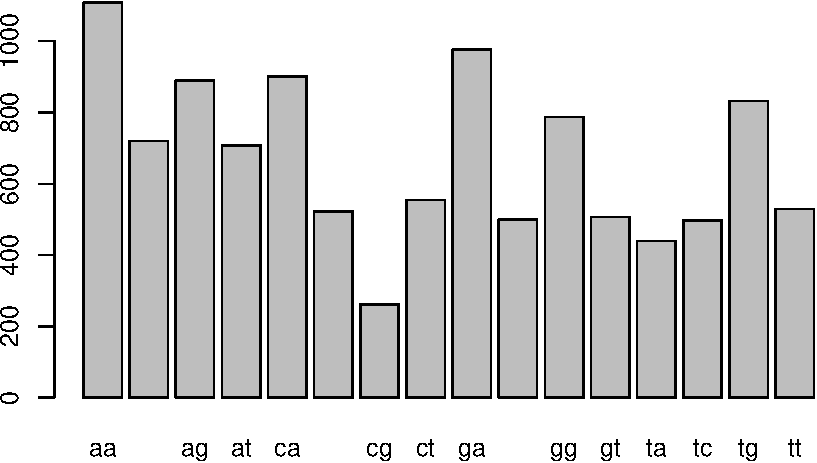
\includegraphics{lbrb_files/figure-latex/unnamed-chunk-58-1.pdf}

We can sort by the number of words using the sort() command

\begin{Shaded}
\begin{Highlighting}[]
\FunctionTok{sort}\NormalTok{(denguetable\_2)}
\end{Highlighting}
\end{Shaded}

\begin{verbatim}
## 
##   cg   ta   tc   gc   gt   cc   tt   ct   at   ac   gg   tg   ag   ca   ga   aa 
##  261  440  497  500  507  523  529  555  708  720  787  832  890  901  976 1108
\end{verbatim}

Let's save over the original object

\begin{Shaded}
\begin{Highlighting}[]
\NormalTok{denguetable\_2 }\OtherTok{\textless{}{-}} \FunctionTok{sort}\NormalTok{(denguetable\_2)}
\end{Highlighting}
\end{Shaded}

\begin{Shaded}
\begin{Highlighting}[]
\FunctionTok{barplot}\NormalTok{(denguetable\_2)}
\end{Highlighting}
\end{Shaded}

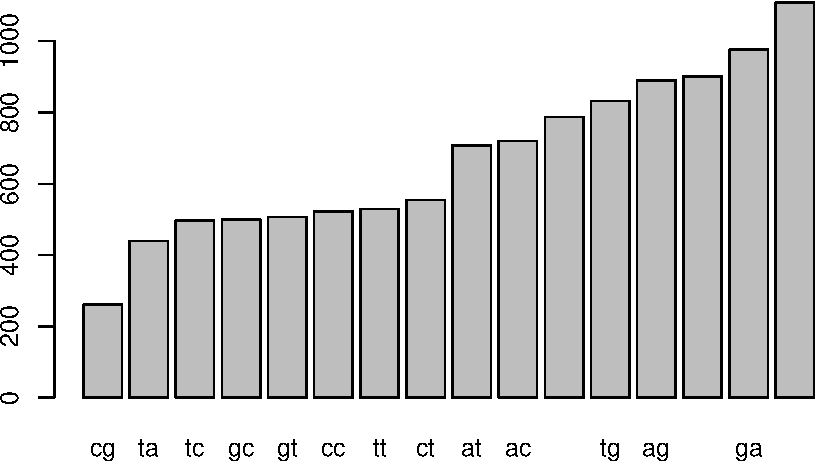
\includegraphics{lbrb_files/figure-latex/unnamed-chunk-61-1.pdf}

R will automatically try to optimize the appearance of the labels on the graph so you may not see all of them; no worries.

R can also make pie charts. Piecharts only really work when there are a few items being plots, like the four bases.

\begin{Shaded}
\begin{Highlighting}[]
\NormalTok{denguetable\_1 }\OtherTok{\textless{}{-}}\NormalTok{ seqinr}\SpecialCharTok{::}\FunctionTok{count}\NormalTok{(dengueseq\_vector,}\DecValTok{1}\NormalTok{)}
\end{Highlighting}
\end{Shaded}

Make a piechart with pie()

\begin{Shaded}
\begin{Highlighting}[]
\FunctionTok{pie}\NormalTok{(denguetable\_1)}
\end{Highlighting}
\end{Shaded}

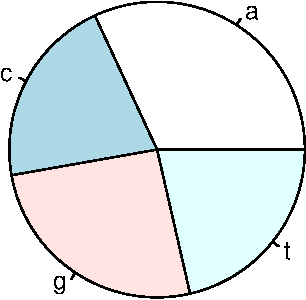
\includegraphics{lbrb_files/figure-latex/unnamed-chunk-63-1.pdf}

\hypertarget{summary}{%
\subsection{Summary}\label{summary}}

In this practical, have learned to use the following R functions:

length() for finding the length of a vector or list
table() for printing out a table of the number of occurrences of each type of item in a vector or list.
These functions belong to the standard installation of R.

You have also learnt the following R functions that belong to the SeqinR package:

GC() for calculating the GC content for a DNA sequence
count() for calculating the number of occurrences of DNA words of a particular length in a DNA sequence

\hypertarget{acknowledgements}{%
\section{Acknowledgements}\label{acknowledgements}}

This is a modification of \href{https://a-little-book-of-r-for-bioinformatics.readthedocs.io/en/latest/src/chapter1.html}{``DNA Sequence Statistics (1)''} from Avril Coghlan's \href{https://a-little-book-of-r-for-bioinformatics.readthedocs.io/en/latest/index.html}{\emph{A little book of R for bioinformatics.}}. Almost all of text and code was originally written by Dr.~Coghlan and distributed under the \href{https://creativecommons.org/licenses/by/3.0/us/}{Creative Commons 3.0} license.

In ``A little book\ldots{}'' Coghlan noted: ``Many of the ideas for the examples and exercises for this chapter were inspired by the Matlab case studies on Haemophilus influenzae (www.computational-genomics.net/case\_studies/haemophilus\_demo.html) and Bacteriophage lambda (\url{http://www.computational-genomics.net/case_studies/lambdaphage_demo.html}) from the website that accompanies the book Introduction to Computational Genomics: a case studies approach by Cristianini and Hahn (Cambridge University Press; www.computational-genomics.net/book/).''

\hypertarget{license}{%
\subsection{License}\label{license}}

The content in this book is licensed under a Creative Commons Attribution 3.0 License.

\url{https://creativecommons.org/licenses/by/3.0/us/}

\hypertarget{exercises}{%
\subsection{Exercises}\label{exercises}}

Answer the following questions, using the R package. For each question, please record your answer, and what you typed into R to get this answer.

Model answers to the exercises are given in Answers to the exercises on DNA Sequence Statistics (1).

\begin{enumerate}
\def\labelenumi{\arabic{enumi}.}
\tightlist
\item
  What are the last twenty nucleotides of the Dengue virus genome sequence?
\item
  What is the length in nucleotides of the genome sequence for the bacterium Mycobacterium leprae strain TN (accession NC\_002677)?
  Note: Mycobacterium leprae is a bacterium that is responsible for causing leprosy, which is classified by the WHO as a neglected tropical disease. As the genome sequence is a DNA sequence, if you are retrieving its sequence via the NCBI website, you will need to look for it in the NCBI Nucleotide database.
\item
  How many of each of the four nucleotides A, C, T and G, and any other symbols, are there in the Mycobacterium leprae TN genome sequence?
  Note: other symbols apart from the four nucleotides A/C/T/G may appear in a sequence. They correspond to positions in the sequence that are are not clearly one base or another and they are due, for example, to sequencing uncertainties. or example, the symbol `N' means `aNy base', while `R' means `A or G' (puRine). There is a table of symbols at www.bioinformatics.org/sms/iupac.html.
\item
  What is the GC content of the \emph{Mycobacterium leprae TN} genome sequence, when (i) all non-A/C/T/G nucleotides are included, (ii) non-A/C/T/G nucleotides are discarded?
  Hint: look at the help page for the GC() function to find out how it deals with non-A/C/T/G nucleotides.
\item
  How many of each of the four nucleotides A, C, T and G are there in the complement of the Mycobacterium leprae TN genome sequence? \emph{Hint}: you will first need to search for a function to calculate the complement of a sequence. Once you have found out what function to use, remember to use the help() function to find out what are the arguments (inputs) and results (outputs) of that function. How does the function deal with symbols other than the four nucleotides A, C, T and G? Are the numbers of As, Cs, Ts, and Gs in the complementary sequence what you would expect?
\item
  How many occurrences of the DNA words CC, CG and GC occur in the Mycobacterium leprae TN genome sequence?
\item
  How many occurrences of the DNA words CC, CG and GC occur in the (i) first 1000 and (ii) last 1000 nucleotides of the Mycobacterium leprae TN genome sequence?
  1.How can you check that the subsequence that you have looked at is 1000 nucleotides long?
\end{enumerate}

\hypertarget{downloading-dna-sequences-with-r}{%
\chapter{Downloading DNA sequences with R}\label{downloading-dna-sequences-with-r}}

This is a modification of \href{https://a-little-book-of-r-for-bioinformatics.readthedocs.io/en/latest/src/chapter1.html}{``DNA Sequence Statistics''} from Avril Coghlan's \href{https://a-little-book-of-r-for-bioinformatics.readthedocs.io/en/latest/index.html}{\emph{A little book of R for bioinformatics.}}. Almost all of text and code was originally written by Dr.~Coghlan and distributed under the \href{https://creativecommons.org/licenses/by/3.0/us/}{Creative Commons 3.0} license.

\hypertarget{functions}{%
\subsection{Functions}\label{functions}}

\begin{itemize}
\tightlist
\item
  library()
\item
  help()
\item
  length
\item
  table
\item
  seqinr::GC
\item
  seqinr::count
\item
  seqinr::write.fasta
\end{itemize}

\hypertarget{softwarewebsites}{%
\subsection{Software/websites}\label{softwarewebsites}}

\begin{itemize}
\tightlist
\item
  www.ncbi.nlm.nih.gov
\item
  Text editor (eg Notepad++, TextWrangler)
\end{itemize}

\hypertarget{r-vocabulary}{%
\subsection{R vocabulary}\label{r-vocabulary}}

\begin{itemize}
\tightlist
\item
  list
\item
  library
\item
  package
\item
  CRAN
\item
  wrapper
\end{itemize}

\hypertarget{file-types}{%
\subsection{File types}\label{file-types}}

\begin{itemize}
\tightlist
\item
  FASTA
\end{itemize}

\hypertarget{bioinformatics-vocabulary}{%
\subsection{Bioinformatics vocabulary}\label{bioinformatics-vocabulary}}

\begin{itemize}
\tightlist
\item
  accession
\item
  NCBI
\item
  NCBI Sequence Database
\item
  EMBL Sequence Database
\item
  FASTA file
\end{itemize}

\hypertarget{organisms-and-sequence-accessions}{%
\subsection{Organisms and Sequence accessions}\label{organisms-and-sequence-accessions}}

Dengue virus: DEN-1, DEN-2, DEN-3, and DEN-4.

The NCBI accessions for the DNA sequences of the DEN-1, DEN-2, DEN-3, and DEN-4 Dengue viruses are NC\_001477, NC\_001474, NC\_001475 and NC\_002640, respectively.

According to Wikipedia

\begin{quote}
``Dengue virus (DENV) is the cause of dengue fever. It is a mosquito-borne, single positive-stranded RNA virus \ldots. Five serotypes of the virus have been found, all of which can cause the full spectrum of disease. Nevertheless, scientists' understanding of dengue virus may be simplistic, as rather than distinct \ldots{} groups, a continuum appears to exist. \ldots{} {[}A{]} study identified 47 strains of dengue virus.'' \url{https://en.wikipedia.org/wiki/Dengue_virus}
\end{quote}

\hypertarget{preliminaries-1}{%
\subsection{Preliminaries}\label{preliminaries-1}}

\begin{Shaded}
\begin{Highlighting}[]
\FunctionTok{library}\NormalTok{(rentrez)}
\FunctionTok{library}\NormalTok{(compbio4all)}
\end{Highlighting}
\end{Shaded}

\hypertarget{dna-sequence-statistics-part-1}{%
\section{DNA Sequence Statistics: Part 1}\label{dna-sequence-statistics-part-1}}

\hypertarget{using-r-for-bioinformatics}{%
\subsection{Using R for Bioinformatics}\label{using-r-for-bioinformatics}}

These tutorials tell you how to use R to carry out simple analyses that are common in bioinformatics and computational biology. In particular, the focus is on computational analysis of biological sequence data such as genome sequences and protein sequences. The programming approaches, however, are broadly generalizable to statistics and data science.

The tutorials assume that the reader has some basic knowledge of biology, but not necessarily of bioinformatics. The focus is to explain simple bioinformatics analysis, and to explain how to carry out these analyses using \emph{R}.

\hypertarget{r-packages-for-bioinformatics-bioconductor-and-seqinr}{%
\subsection{R packages for bioinformatics: Bioconductor and SeqinR}\label{r-packages-for-bioinformatics-bioconductor-and-seqinr}}

Many authors have written \emph{R} packages for performing a wide variety of analyses. These do not come with the standard \emph{R} installation, but must be installed and loaded as ``add-ons''. Loading the dayoff package will automatically load most of the packages we need.

Bioinformaticians have written numerous specialized packages for R. In this tutorial, you will learn to use some of the function in the \href{https://cran.r-project.org/web/packages/seqinr/index.html}{\emph{SeqinR}} package to to carry out simple analyses of DNA sequences. (SeqinR can retrieve sequences from a DNA sequence database, but this has largely been replaced by the functions in the package \emph{rentrez})

Many well-known bioinformatics packages for \emph{R} are in the Bioconductor set of R packages (www.bioconductor.org), which contains packages with many \emph{R} functions for analyzing biological data sets such as microarray data; and the \href{https://cran.r-project.org/web/packages/seqinr/index.html}{\emph{SeqinR}} package from CRAN, which contains R functions for obtaining sequences from DNA and protein sequence databases, and for analyzing DNA and protein sequences.

SequinR will automatically load when you load dayoff. For instructions on how to install an R package on your own see \href{https://a-little-book-of-r-for-bioinformatics.readthedocs.io/en/latest/src/installr.html}{How to install an R package}.

We will also use functions from the \emph{rentrez} and \emph{ape} packages. Both of these also are loaded automatically by the dayoff package.

Remember that you can ask for more information about a particular R command by using the \texttt{help()\ eval\ =\ F} function. For example, to ask for more information about the \texttt{library()\ eval\ =\ F\ function}, you can type:

\begin{Shaded}
\begin{Highlighting}[]
\FunctionTok{help}\NormalTok{(}\StringTok{"library"}\NormalTok{)}
\end{Highlighting}
\end{Shaded}

You can also do this

\begin{Shaded}
\begin{Highlighting}[]
\NormalTok{?library}
\end{Highlighting}
\end{Shaded}

\hypertarget{fasta-file-format}{%
\subsection{FASTA file format}\label{fasta-file-format}}

The FASTA format is a simple and widely used format for storing biological (eg DNA or protein) sequences. It was first used by the \href{https://en.wikipedia.org/wiki/FASTA}{FASTA program} for sequence alignment in the 1980s and has been adopted as standard by many other programs.

FASTA files begin with a single-line description starting with a greater-than sign ``\textgreater{}'' character, followed on the next line with the sequences. Here is an example of a FASTA file. (The cat() command is just a text display function used format the text when you run the code).

\begin{verbatim}
## A06852 183 residues MPRLFSYLLGVWLLLSQLPREIPGQSTNDFIKACGRELVRLWVEICGSVSWGRTALSLEEPQLETGPPAETMPSSITKDAEILKMMLEFVPNLPQELKATLSERQPSLRELQQSASKDSNLNFEEFKKIILNRQNEAEDKSLLELKNLGLDKHSRKKRLFRMTLSEKCCQVGCIRKDIARLC
\end{verbatim}

\hypertarget{the-ncbi-sequence-database}{%
\subsection{The NCBI sequence database}\label{the-ncbi-sequence-database}}

The \href{www.ncbi.nlm.nih.gov}{National Centre for Biotechnology Information (NCBI)} in the US maintains a huge database of all the DNA and protein sequence data that has been collected, the NCBI Sequence Database. This also a similar database in Europe, the \href{www.ebi.ac.uk/embl}{European Molecular Biology Laboratory (EMBL) Sequence Database}, and also a similar database in Japan, the \href{www.ddbj.nig.ac.jp}{DNA Data Bank of Japan (DDBJ)}. These three databases exchange data every night, so at any one point in time, they contain almost identical data.

Each sequence in the NCBI Sequence Database is stored in a separate \textbf{record}, and is assigned a unique identifier that can be used to refer to that sequence record. The identifier is known as an \textbf{accession}, and consists of a mixture of numbers and letters. For example, Dengue virus causes Dengue fever, which is classified as a neglected tropical disease by the World Health Organization (WHO), is classified by any one of four types of Dengue virus: DEN-1, DEN-2, DEN-3, and DEN-4. The NCBI accessions for the DNA sequences of the DEN-1, DEN-2, DEN-3, and DEN-4 Dengue viruses are NC\_001477, NC\_001474, NC\_001475 and NC\_002640, respectively.

Note that because the NCBI Sequence Database, the EMBL Sequence Database, and DDBJ exchange data every night, the DEN-1 (and DEN-2, DEN-3, DEN-4) Dengue virus sequence will be present in all three databases, but it will have different accessions in each database, as they each use their own numbering systems for referring to their own sequence records.

\hypertarget{retrieving-genome-sequence-data-using-rentrez}{%
\subsection{Retrieving genome sequence data using rentrez}\label{retrieving-genome-sequence-data-using-rentrez}}

You can retrieve sequence data from NCBI directly from \emph{R} using the \emph{rentrez} package. The DEN-1 Dengue virus genome sequence has NCBI accession NC\_001477. To retrieve a sequence with a particular NCBI accession, you can use an R function entrez\_fetch() from the rentrez package.

\begin{Shaded}
\begin{Highlighting}[]
\NormalTok{dengueseq\_fasta }\OtherTok{\textless{}{-}} \FunctionTok{entrez\_fetch}\NormalTok{(}\AttributeTok{db =} \StringTok{"nucleotide"}\NormalTok{, }
                          \AttributeTok{id =} \StringTok{"NC\_001477"}\NormalTok{, }
                          \AttributeTok{rettype =} \StringTok{"fasta"}\NormalTok{)}
\end{Highlighting}
\end{Shaded}

Note that the ``\emph{" in the name is just an arbitrary way to separate two words. Another common format would be dengueseq.fasta. Some people like dengueseqFasta, called "camel case" because the capital letter makes a hump in the middle of the word. Underscores are becoming most common and are favored by developers associated with RStudio and the "tidyverse" of packages that many data scientists user. I switch between "." and "}'' as separators, usually favoring "\_" for function names and ``.'' for objects; I personally find camel case hard to read and harder to type.

Ok, so what exactly have we done when we made dengueseq\_fasta? We have an R object ``dengueseq\_fasta'' which has the sequence linked to the accession number ``NC\_001477.'' So where is the sequence, and what is it?

First, what is it?

How big is it? Try the dim() and length() commands and see which one works. Do you know why?

The size of the object is 1. Why is this? We'll use another function to explore that. Thing about this: how many pieces of unique information are in the dengueseq object? In what sense is there only 1 piece of information?

If we want to actually we can type just type ``dengueseq\_fasta'' and press enter. This will print the WHOLE genomic sequence out but it will probably run of your screen.

\begin{Shaded}
\begin{Highlighting}[]
\NormalTok{dengueseq\_fasta}
\end{Highlighting}
\end{Shaded}

\begin{verbatim}
## [1] ">NC_001477.1 Dengue virus 1, complete genome\nAGTTGTTAGTCTACGTGGACCGACAAGAACAGTTTCGAATCGGAAGCTTGCTTAACGTAGTTCTAACAGT\nTTTTTATTAGAGAGCAGATCTCTGATGAACAACCAACGGAAAAAGACGGGTCGACCGTCTTTCAATATGC\nTGAAACGCGCGAGAAACCGCGTGTCAACTGTTTCACAGTTGGCGAAGAGATTCTCAAAAGGATTGCTTTC\nAGGCCAAGGACCCATGAAATTGGTGATGGCTTTTATAGCATTCCTAAGATTTCTAGCCATACCTCCAACA\nGCAGGAATTTTGGCTAGATGGGGCTCATTCAAGAAGAATGGAGCGATCAAAGTGTTACGGGGTTTCAAGA\nAAGAAATCTCAAACATGTTGAACATAATGAACAGGAGGAAAAGATCTGTGACCATGCTCCTCATGCTGCT\nGCCCACAGCCCTGGCGTTCCATCTGACCACCCGAGGGGGAGAGCCGCACATGATAGTTAGCAAGCAGGAA\nAGAGGAAAATCACTTTTGTTTAAGACCTCTGCAGGTGTCAACATGTGCACCCTTATTGCAATGGATTTGG\nGAGAGTTATGTGAGGACACAATGACCTACAAATGCCCCCGGATCACTGAGACGGAACCAGATGACGTTGA\nCTGTTGGTGCAATGCCACGGAGACATGGGTGACCTATGGAACATGTTCTCAAACTGGTGAACACCGACGA\nGACAAACGTTCCGTCGCACTGGCACCACACGTAGGGCTTGGTCTAGAAACAAGAACCGAAACGTGGATGT\nCCTCTGAAGGCGCTTGGAAACAAATACAAAAAGTGGAGACCTGGGCTCTGAGACACCCAGGATTCACGGT\nGATAGCCCTTTTTCTAGCACATGCCATAGGAACATCCATCACCCAGAAAGGGATCATTTTTATTTTGCTG\nATGCTGGTAACTCCATCCATGGCCATGCGGTGCGTGGGAATAGGCAACAGAGACTTCGTGGAAGGACTGT\nCAGGAGCTACGTGGGTGGATGTGGTACTGGAGCATGGAAGTTGCGTCACTACCATGGCAAAAGACAAACC\nAACACTGGACATTGAACTCTTGAAGACGGAGGTCACAAACCCTGCCGTCCTGCGCAAACTGTGCATTGAA\nGCTAAAATATCAAACACCACCACCGATTCGAGATGTCCAACACAAGGAGAAGCCACGCTGGTGGAAGAAC\nAGGACACGAACTTTGTGTGTCGACGAACGTTCGTGGACAGAGGCTGGGGCAATGGTTGTGGGCTATTCGG\nAAAAGGTAGCTTAATAACGTGTGCTAAGTTTAAGTGTGTGACAAAACTGGAAGGAAAGATAGTCCAATAT\nGAAAACTTAAAATATTCAGTGATAGTCACCGTACACACTGGAGACCAGCACCAAGTTGGAAATGAGACCA\nCAGAACATGGAACAACTGCAACCATAACACCTCAAGCTCCCACGTCGGAAATACAGCTGACAGACTACGG\nAGCTCTAACATTGGATTGTTCACCTAGAACAGGGCTAGACTTTAATGAGATGGTGTTGTTGACAATGAAA\nAAAAAATCATGGCTCGTCCACAAACAATGGTTTCTAGACTTACCACTGCCTTGGACCTCGGGGGCTTCAA\nCATCCCAAGAGACTTGGAATAGACAAGACTTGCTGGTCACATTTAAGACAGCTCATGCAAAAAAGCAGGA\nAGTAGTCGTACTAGGATCACAAGAAGGAGCAATGCACACTGCGTTGACTGGAGCGACAGAAATCCAAACG\nTCTGGAACGACAACAATTTTTGCAGGACACCTGAAATGCAGATTAAAAATGGATAAACTGATTTTAAAAG\nGGATGTCATATGTAATGTGCACAGGGTCATTCAAGTTAGAGAAGGAAGTGGCTGAGACCCAGCATGGAAC\nTGTTCTAGTGCAGGTTAAATACGAAGGAACAGATGCACCATGCAAGATCCCCTTCTCGTCCCAAGATGAG\nAAGGGAGTAACCCAGAATGGGAGATTGATAACAGCCAACCCCATAGTCACTGACAAAGAAAAACCAGTCA\nACATTGAAGCGGAGCCACCTTTTGGTGAGAGCTACATTGTGGTAGGAGCAGGTGAAAAAGCTTTGAAACT\nAAGCTGGTTCAAGAAGGGAAGCAGTATAGGGAAAATGTTTGAAGCAACTGCCCGTGGAGCACGAAGGATG\nGCCATCCTGGGAGACACTGCATGGGACTTCGGTTCTATAGGAGGGGTGTTCACGTCTGTGGGAAAACTGA\nTACACCAGATTTTTGGGACTGCGTATGGAGTTTTGTTCAGCGGTGTTTCTTGGACCATGAAGATAGGAAT\nAGGGATTCTGCTGACATGGCTAGGATTAAACTCAAGGAGCACGTCCCTTTCAATGACGTGTATCGCAGTT\nGGCATGGTCACACTGTACCTAGGAGTCATGGTTCAGGCGGACTCGGGATGTGTAATCAACTGGAAAGGCA\nGAGAACTCAAATGTGGAAGCGGCATTTTTGTCACCAATGAAGTCCACACCTGGACAGAGCAATATAAATT\nCCAGGCCGACTCCCCTAAGAGACTATCAGCGGCCATTGGGAAGGCATGGGAGGAGGGTGTGTGTGGAATT\nCGATCAGCCACTCGTCTCGAGAACATCATGTGGAAGCAAATATCAAATGAATTAAACCACATCTTACTTG\nAAAATGACATGAAATTTACAGTGGTCGTAGGAGACGTTAGTGGAATCTTGGCCCAAGGAAAGAAAATGAT\nTAGGCCACAACCCATGGAACACAAATACTCGTGGAAAAGCTGGGGAAAAGCCAAAATCATAGGAGCAGAT\nGTACAGAATACCACCTTCATCATCGACGGCCCAAACACCCCAGAATGCCCTGATAACCAAAGAGCATGGA\nACATTTGGGAAGTTGAAGACTATGGATTTGGAATTTTCACGACAAACATATGGTTGAAATTGCGTGACTC\nCTACACTCAAGTGTGTGACCACCGGCTAATGTCAGCTGCCATCAAGGATAGCAAAGCAGTCCATGCTGAC\nATGGGGTACTGGATAGAAAGTGAAAAGAACGAGACTTGGAAGTTGGCAAGAGCCTCCTTCATAGAAGTTA\nAGACATGCATCTGGCCAAAATCCCACACTCTATGGAGCAATGGAGTCCTGGAAAGTGAGATGATAATCCC\nAAAGATATATGGAGGACCAATATCTCAGCACAACTACAGACCAGGATATTTCACACAAACAGCAGGGCCG\nTGGCACTTGGGCAAGTTAGAACTAGATTTTGATTTATGTGAAGGTACCACTGTTGTTGTGGATGAACATT\nGTGGAAATCGAGGACCATCTCTTAGAACCACAACAGTCACAGGAAAGACAATCCATGAATGGTGCTGTAG\nATCTTGCACGTTACCCCCCCTACGTTTCAAAGGAGAAGACGGGTGCTGGTACGGCATGGAAATCAGACCA\nGTCAAGGAGAAGGAAGAGAACCTAGTTAAGTCAATGGTCTCTGCAGGGTCAGGAGAAGTGGACAGTTTTT\nCACTAGGACTGCTATGCATATCAATAATGATCGAAGAGGTAATGAGATCCAGATGGAGCAGAAAAATGCT\nGATGACTGGAACATTGGCTGTGTTCCTCCTTCTCACAATGGGACAATTGACATGGAATGATCTGATCAGG\nCTATGTATCATGGTTGGAGCCAACGCTTCAGACAAGATGGGGATGGGAACAACGTACCTAGCTTTGATGG\nCCACTTTCAGAATGAGACCAATGTTCGCAGTCGGGCTACTGTTTCGCAGATTAACATCTAGAGAAGTTCT\nTCTTCTTACAGTTGGATTGAGTCTGGTGGCATCTGTAGAACTACCAAATTCCTTAGAGGAGCTAGGGGAT\nGGACTTGCAATGGGCATCATGATGTTGAAATTACTGACTGATTTTCAGTCACATCAGCTATGGGCTACCT\nTGCTGTCTTTAACATTTGTCAAAACAACTTTTTCATTGCACTATGCATGGAAGACAATGGCTATGATACT\nGTCAATTGTATCTCTCTTCCCTTTATGCCTGTCCACGACTTCTCAAAAAACAACATGGCTTCCGGTGTTG\nCTGGGATCTCTTGGATGCAAACCACTAACCATGTTTCTTATAACAGAAAACAAAATCTGGGGAAGGAAAA\nGCTGGCCTCTCAATGAAGGAATTATGGCTGTTGGAATAGTTAGCATTCTTCTAAGTTCACTTCTCAAGAA\nTGATGTGCCACTAGCTGGCCCACTAATAGCTGGAGGCATGCTAATAGCATGTTATGTCATATCTGGAAGC\nTCGGCCGATTTATCACTGGAGAAAGCGGCTGAGGTCTCCTGGGAAGAAGAAGCAGAACACTCTGGTGCCT\nCACACAACATACTAGTGGAGGTCCAAGATGATGGAACCATGAAGATAAAGGATGAAGAGAGAGATGACAC\nACTCACCATTCTCCTCAAAGCAACTCTGCTAGCAATCTCAGGGGTATACCCAATGTCAATACCGGCGACC\nCTCTTTGTGTGGTATTTTTGGCAGAAAAAGAAACAGAGATCAGGAGTGCTATGGGACACACCCAGCCCTC\nCAGAAGTGGAAAGAGCAGTCCTTGATGATGGCATTTATAGAATTCTCCAAAGAGGATTGTTGGGCAGGTC\nTCAAGTAGGAGTAGGAGTTTTTCAAGAAGGCGTGTTCCACACAATGTGGCACGTCACCAGGGGAGCTGTC\nCTCATGTACCAAGGGAAGAGACTGGAACCAAGTTGGGCCAGTGTCAAAAAAGACTTGATCTCATATGGAG\nGAGGTTGGAGGTTTCAAGGATCCTGGAACGCGGGAGAAGAAGTGCAGGTGATTGCTGTTGAACCGGGGAA\nGAACCCCAAAAATGTACAGACAGCGCCGGGTACCTTCAAGACCCCTGAAGGCGAAGTTGGAGCCATAGCT\nCTAGACTTTAAACCCGGCACATCTGGATCTCCTATCGTGAACAGAGAGGGAAAAATAGTAGGTCTTTATG\nGAAATGGAGTGGTGACAACAAGTGGTACCTACGTCAGTGCCATAGCTCAAGCTAAAGCATCACAAGAAGG\nGCCTCTACCAGAGATTGAGGACGAGGTGTTTAGGAAAAGAAACTTAACAATAATGGACCTACATCCAGGA\nTCGGGAAAAACAAGAAGATACCTTCCAGCCATAGTCCGTGAGGCCATAAAAAGAAAGCTGCGCACGCTAG\nTCTTAGCTCCCACAAGAGTTGTCGCTTCTGAAATGGCAGAGGCGCTCAAGGGAATGCCAATAAGGTATCA\nGACAACAGCAGTGAAGAGTGAACACACGGGAAAGGAGATAGTTGACCTTATGTGTCACGCCACTTTCACT\nATGCGTCTCCTGTCTCCTGTGAGAGTTCCCAATTATAATATGATTATCATGGATGAAGCACATTTTACCG\nATCCAGCCAGCATAGCAGCCAGAGGGTATATCTCAACCCGAGTGGGTATGGGTGAAGCAGCTGCGATTTT\nCATGACAGCCACTCCCCCCGGATCGGTGGAGGCCTTTCCACAGAGCAATGCAGTTATCCAAGATGAGGAA\nAGAGACATTCCTGAAAGATCATGGAACTCAGGCTATGACTGGATCACTGATTTCCCAGGTAAAACAGTCT\nGGTTTGTTCCAAGCATCAAATCAGGAAATGACATTGCCAACTGTTTAAGAAAGAATGGGAAACGGGTGGT\nCCAATTGAGCAGAAAAACTTTTGACACTGAGTACCAGAAAACAAAAAATAACGACTGGGACTATGTTGTC\nACAACAGACATATCCGAAATGGGAGCAAACTTCCGAGCCGACAGGGTAATAGACCCGAGGCGGTGCCTGA\nAACCGGTAATACTAAAAGATGGCCCAGAGCGTGTCATTCTAGCCGGACCGATGCCAGTGACTGTGGCTAG\nCGCCGCCCAGAGGAGAGGAAGAATTGGAAGGAACCAAAATAAGGAAGGCGATCAGTATATTTACATGGGA\nCAGCCTCTAAACAATGATGAGGACCACGCCCATTGGACAGAAGCAAAAATGCTCCTTGACAACATAAACA\nCACCAGAAGGGATTATCCCAGCCCTCTTTGAGCCGGAGAGAGAAAAGAGTGCAGCAATAGACGGGGAATA\nCAGACTACGGGGTGAAGCGAGGAAAACGTTCGTGGAGCTCATGAGAAGAGGAGATCTACCTGTCTGGCTA\nTCCTACAAAGTTGCCTCAGAAGGCTTCCAGTACTCCGACAGAAGGTGGTGCTTTGATGGGGAAAGGAACA\nACCAGGTGTTGGAGGAGAACATGGACGTGGAGATCTGGACAAAAGAAGGAGAAAGAAAGAAACTACGACC\nCCGCTGGCTGGATGCCAGAACATACTCTGACCCACTGGCTCTGCGCGAATTCAAAGAGTTCGCAGCAGGA\nAGAAGAAGCGTCTCAGGTGACCTAATATTAGAAATAGGGAAACTTCCACAACATTTAACGCAAAGGGCCC\nAGAACGCCTTGGACAATCTGGTTATGTTGCACAACTCTGAACAAGGAGGAAAAGCCTATAGACACGCCAT\nGGAAGAACTACCAGACACCATAGAAACGTTAATGCTCCTAGCTTTGATAGCTGTGCTGACTGGTGGAGTG\nACGTTGTTCTTCCTATCAGGAAGGGGTCTAGGAAAAACATCCATTGGCCTACTCTGCGTGATTGCCTCAA\nGTGCACTGTTATGGATGGCCAGTGTGGAACCCCATTGGATAGCGGCCTCTATCATACTGGAGTTCTTTCT\nGATGGTGTTGCTTATTCCAGAGCCGGACAGACAGCGCACTCCACAAGACAACCAGCTAGCATACGTGGTG\nATAGGTCTGTTATTCATGATATTGACAGTGGCAGCCAATGAGATGGGATTACTGGAAACCACAAAGAAGG\nACCTGGGGATTGGTCATGCAGCTGCTGAAAACCACCATCATGCTGCAATGCTGGACGTAGACCTACATCC\nAGCTTCAGCCTGGACTCTCTATGCAGTGGCCACAACAATTATCACTCCCATGATGAGACACACAATTGAA\nAACACAACGGCAAATATTTCCCTGACAGCTATTGCAAACCAGGCAGCTATATTGATGGGACTTGACAAGG\nGATGGCCAATATCAAAGATGGACATAGGAGTTCCACTTCTCGCCTTGGGGTGCTATTCTCAGGTGAACCC\nGCTGACGCTGACAGCGGCGGTATTGATGCTAGTGGCTCATTATGCCATAATTGGACCCGGACTGCAAGCA\nAAAGCTACTAGAGAAGCTCAAAAAAGGACAGCAGCCGGAATAATGAAAAACCCAACTGTCGACGGGATCG\nTTGCAATAGATTTGGACCCTGTGGTTTACGATGCAAAATTTGAAAAACAGCTAGGCCAAATAATGTTGTT\nGATACTTTGCACATCACAGATCCTCCTGATGCGGACCACATGGGCCTTGTGTGAATCCATCACACTAGCC\nACTGGACCTCTGACTACGCTTTGGGAGGGATCTCCAGGAAAATTCTGGAACACCACGATAGCGGTGTCCA\nTGGCAAACATTTTTAGGGGAAGTTATCTAGCAGGAGCAGGTCTGGCCTTTTCATTAATGAAATCTCTAGG\nAGGAGGTAGGAGAGGCACGGGAGCCCAAGGGGAAACACTGGGAGAAAAATGGAAAAGACAGCTAAACCAA\nTTGAGCAAGTCAGAATTCAACACTTACAAAAGGAGTGGGATTATAGAGGTGGATAGATCTGAAGCCAAAG\nAGGGGTTAAAAAGAGGAGAAACGACTAAACACGCAGTGTCGAGAGGAACGGCCAAACTGAGGTGGTTTGT\nGGAGAGGAACCTTGTGAAACCAGAAGGGAAAGTCATAGACCTCGGTTGTGGAAGAGGTGGCTGGTCATAT\nTATTGCGCTGGGCTGAAGAAAGTCACAGAAGTGAAAGGATACACGAAAGGAGGACCTGGACATGAGGAAC\nCAATCCCAATGGCAACCTATGGATGGAACCTAGTAAAGCTATACTCCGGGAAAGATGTATTCTTTACACC\nACCTGAGAAATGTGACACCCTCTTGTGTGATATTGGTGAGTCCTCTCCGAACCCAACTATAGAAGAAGGA\nAGAACGTTACGTGTTCTAAAGATGGTGGAACCATGGCTCAGAGGAAACCAATTTTGCATAAAAATTCTAA\nATCCCTATATGCCGAGTGTGGTAGAAACTTTGGAGCAAATGCAAAGAAAACATGGAGGAATGCTAGTGCG\nAAATCCACTCTCAAGAAACTCCACTCATGAAATGTACTGGGTTTCATGTGGAACAGGAAACATTGTGTCA\nGCAGTAAACATGACATCTAGAATGCTGCTAAATCGATTCACAATGGCTCACAGGAAGCCAACATATGAAA\nGAGACGTGGACTTAGGCGCTGGAACAAGACATGTGGCAGTAGAACCAGAGGTGGCCAACCTAGATATCAT\nTGGCCAGAGGATAGAGAATATAAAAAATGAACACAAATCAACATGGCATTATGATGAGGACAATCCATAC\nAAAACATGGGCCTATCATGGATCATATGAGGTCAAGCCATCAGGATCAGCCTCATCCATGGTCAATGGTG\nTGGTGAGACTGCTAACCAAACCATGGGATGTCATTCCCATGGTCACACAAATAGCCATGACTGACACCAC\nACCCTTTGGACAACAGAGGGTGTTTAAAGAGAAAGTTGACACGCGTACACCAAAAGCGAAACGAGGCACA\nGCACAAATTATGGAGGTGACAGCCAGGTGGTTATGGGGTTTTCTCTCTAGAAACAAAAAACCCAGAATCT\nGCACAAGAGAGGAGTTCACAAGAAAAGTCAGGTCAAACGCAGCTATTGGAGCAGTGTTCGTTGATGAAAA\nTCAATGGAACTCAGCAAAAGAGGCAGTGGAAGATGAACGGTTCTGGGACCTTGTGCACAGAGAGAGGGAG\nCTTCATAAACAAGGAAAATGTGCCACGTGTGTCTACAACATGATGGGAAAGAGAGAGAAAAAATTAGGAG\nAGTTCGGAAAGGCAAAAGGAAGTCGCGCAATATGGTACATGTGGTTGGGAGCGCGCTTTTTAGAGTTTGA\nAGCCCTTGGTTTCATGAATGAAGATCACTGGTTCAGCAGAGAGAATTCACTCAGTGGAGTGGAAGGAGAA\nGGACTCCACAAACTTGGATACATACTCAGAGACATATCAAAGATTCCAGGGGGAAATATGTATGCAGATG\nACACAGCCGGATGGGACACAAGAATAACAGAGGATGATCTTCAGAATGAGGCCAAAATCACTGACATCAT\nGGAACCTGAACATGCCCTATTGGCCACGTCAATCTTTAAGCTAACCTACCAAAACAAGGTAGTAAGGGTG\nCAGAGACCAGCGAAAAATGGAACCGTGATGGATGTCATATCCAGACGTGACCAGAGAGGAAGTGGACAGG\nTTGGAACCTATGGCTTAAACACCTTCACCAACATGGAGGCCCAACTAATAAGACAAATGGAGTCTGAGGG\nAATCTTTTCACCCAGCGAATTGGAAACCCCAAATCTAGCCGAAAGAGTCCTCGACTGGTTGAAAAAACAT\nGGCACCGAGAGGCTGAAAAGAATGGCAATCAGTGGAGATGACTGTGTGGTGAAACCAATCGATGACAGAT\nTTGCAACAGCCTTAACAGCTTTGAATGACATGGGAAAGGTAAGAAAAGACATACCGCAATGGGAACCTTC\nAAAAGGATGGAATGATTGGCAACAAGTGCCTTTCTGTTCACACCATTTCCACCAGCTGATTATGAAGGAT\nGGGAGGGAGATAGTGGTGCCATGCCGCAACCAAGATGAACTTGTAGGTAGGGCCAGAGTATCACAAGGCG\nCCGGATGGAGCTTGAGAGAAACTGCATGCCTAGGCAAGTCATATGCACAAATGTGGCAGCTGATGTACTT\nCCACAGGAGAGACTTGAGATTAGCGGCTAATGCTATCTGTTCAGCCGTTCCAGTTGATTGGGTCCCAACC\nAGCCGCACCACCTGGTCGATCCATGCCCACCATCAATGGATGACAACAGAAGACATGTTGTCAGTGTGGA\nATAGGGTTTGGATAGAGGAAAACCCATGGATGGAGGACAAGACTCATGTGTCCAGTTGGGAAGACGTTCC\nATACCTAGGAAAAAGGGAAGATCAATGGTGTGGTTCCCTAATAGGCTTAACAGCACGAGCCACCTGGGCC\nACCAACATACAAGTGGCCATAAACCAAGTGAGAAGGCTCATTGGGAATGAGAATTATCTAGACTTCATGA\nCATCAATGAAGAGATTCAAAAACGAGAGTGATCCCGAAGGGGCACTCTGGTAAGCCAACTCATTCACAAA\nATAAAGGAAAATAAAAAATCAAACAAGGCAAGAAGTCAGGCCGGATTAAGCCATAGCACGGTAAGAGCTA\nTGCTGCCTGTGAGCCCCGTCCAAGGACGTAAAATGAAGTCAGGCCGAAAGCCACGGTTCGAGCAAGCCGT\nGCTGCCTGTAGCTCCATCGTGGGGATGTAAAAACCCGGGAGGCTGCAAACCATGGAAGCTGTACGCATGG\nGGTAGCAGACTAGTGGTTAGAGGAGACCCCTCCCAAGACACAACGCAGCAGCGGGGCCCAACACCAGGGG\nAAGCTGTACCCTGGTGGTAAGGACTAGAGGTTAGAGGAGACCCCCCGCACAACAACAAACAGCATATTGA\nCGCTGGGAGAGACCAGAGATCCTGCTGTCTCTACAGCATCATTCCAGGCACAGAACGCCAAAAAATGGAA\nTGGTGCTGTTGAATCAACAGGTTCT\n\n"
\end{verbatim}

This is a whole genome sequence, but its stored as single entry in a vector, so length() just tells us how many entries there are in the vector, which is just! If we want to actually know how long the sequence is, we need to use the function nchar()

\begin{Shaded}
\begin{Highlighting}[]
\FunctionTok{nchar}\NormalTok{(dengueseq\_fasta)}
\end{Highlighting}
\end{Shaded}

\begin{verbatim}
## [1] 10935
\end{verbatim}

If we want to see just part of the sequence we can use the strtrim() function. Before you run the code below, predict what the 100 means.

\begin{verbatim}
## [1] ">NC_001477.1 Dengue virus 1, complete genome\nAGTTGTTAGTCTACGTGGACCGACAAGAACAGTTTCGAATCGGAAGCTTGCTTAA"
\end{verbatim}

Note that at the end of the name is a slah follwed by an n, which indicates to the computer that this is a newline; this is read by text editor, but is ignored by R in this context.

\begin{verbatim}
## [1] ">NC_001477.1 Dengue virus 1, complete genome\n"
\end{verbatim}

After the ``\textbackslash n'' will begin the sequence, which will continue on for a LOOOOOONG way. Let's just print a little bit.

\begin{verbatim}
## [1] ">NC_001477.1 Dengue virus 1, complete genome\nAGTTGTT"
\end{verbatim}

Let's print some more. Do you notice anything beside A, T, C and G in the sequence?

\begin{Shaded}
\begin{Highlighting}[]
\FunctionTok{strtrim}\NormalTok{(dengueseq\_fasta, }\DecValTok{200}\NormalTok{)}
\end{Highlighting}
\end{Shaded}

\begin{verbatim}
## [1] ">NC_001477.1 Dengue virus 1, complete genome\nAGTTGTTAGTCTACGTGGACCGACAAGAACAGTTTCGAATCGGAAGCTTGCTTAACGTAGTTCTAACAGT\nTTTTTATTAGAGAGCAGATCTCTGATGAACAACCAACGGAAAAAGACGGGTCGACCGTCTTTCAATATGC\nTGAAACGCGCGAG"
\end{verbatim}

Now that we a sense of what we're looking at let's explore the dengueseq\_fasta a bit more.

We can find out more information about what it is using the class() command.

\begin{Shaded}
\begin{Highlighting}[]
\FunctionTok{class}\NormalTok{(dengueseq\_fasta)}
\end{Highlighting}
\end{Shaded}

\begin{verbatim}
## [1] "character"
\end{verbatim}

Many things in R are vectors so we can ask R is.vector()

Yup, that's true.

Ok, let's see what else. A handy though often verbose command is is(), which tells us what an object, well, what it is:

There is a lot here but if you scan for some key words you will see ``character'' and ``vector'' at the top. The other stuff you can ignore. The first two things, though, tell us the dengueseq\_fasta is a \textbf{vector} of the class \textbf{character}: a \textbf{character vector}.

Another handy function is str(), which gives us a peak at the context and structure of an R object. This is most useful when you are working in the R console or with dataframes, but is a useful function to run on all R objects. How does this output differ from other ways we've displayed dengueseq\_fasta?

We know it contains character data - how many? nchar() for ``number of characters'' answers that:

\begin{Shaded}
\begin{Highlighting}[]
\FunctionTok{nchar}\NormalTok{(dengueseq\_fasta)}
\end{Highlighting}
\end{Shaded}

\begin{verbatim}
## [1] 10935
\end{verbatim}

\hypertarget{convert-fasta-sequence-to-an-r-variable}{%
\section{Convert FASTA sequence to an R variable}\label{convert-fasta-sequence-to-an-r-variable}}

We can't actually do much with the contents of the dengueseq\_fasta we downloaded with the rentrez package except read them. If we want do address some biological questions with the data we need is to convert it into a data structure R can work with.\\
There are several things we need to remove:

\begin{enumerate}
\def\labelenumi{\arabic{enumi}.}
\tightlist
\item
  The \textbf{meta data} line ``\textgreater NC\_001477.1 Dengue virus 1, complete genome'' (metadata is ``data'' about data, such as where it came from, what it is, who made it, etc.).
\item
  All the ``\textbackslash n'' that show up in the file (these are the line breaks).
\item
  Put each nucleotide of the sequence into its own spot in a vector.
\end{enumerate}

There are functions that can do this automatically, but I haven't found one I like, and walking through this will help you understand the types of operations you can do on text data.

The first two steps involve removing things from the existing \textbf{character string} that contains the sequence. The third step will split the single continuous character string like ``AGTTGTTAGTCTACGT\ldots{}'' into a \textbf{character vector} like c(``A'',``G'',``T'',``T'',``G'',``T'',``T'',``A'',``G'',``T'',``C'',``T'',``A'',``C'',``G'',``T''\ldots), where each element of the vector is a single character.

The second item is the easiest to take care of. R and many programming languages have tools called \textbf{regular expressions} that allow you to manipulate text. R has a function called gsub() which allows you to substitute or delete character data from a string. First I'll remove all those ``\textbackslash n'' values.

\begin{Shaded}
\begin{Highlighting}[]
\NormalTok{dengueseq\_vector }\OtherTok{\textless{}{-}} \FunctionTok{gsub}\NormalTok{(}\StringTok{"}\SpecialCharTok{\textbackslash{}\textbackslash{}}\StringTok{n"}\NormalTok{, }\StringTok{""}\NormalTok{, dengueseq\_fasta)}
\end{Highlighting}
\end{Shaded}

We can use strtrim() to see if it worked

Now for the metadata header. This is a bit complex, but the following code is going to take all the that occurs before the beginning of the sequence (``AGTTGTTAGTC'') and delete it.

First, I'll define what I want to get rid of in an R object

\begin{Shaded}
\begin{Highlighting}[]
\NormalTok{header. }\OtherTok{\textless{}{-}} \StringTok{"\textgreater{}NC\_001477.1 Dengue virus 1, complete genome"}
\end{Highlighting}
\end{Shaded}

Now I'll get rid of it.

\begin{Shaded}
\begin{Highlighting}[]
\NormalTok{dengueseq\_vector }\OtherTok{\textless{}{-}} \FunctionTok{gsub}\NormalTok{(header.,}\StringTok{""}\NormalTok{, dengueseq\_vector)}
\end{Highlighting}
\end{Shaded}

See if it worked:

Now the more complex part. We need to split up a continuous string of letters into a vector. This can be done with the str\_split() function (``string split'') from the stringr package. The notation stringr::str\_split mean ``use the str\_split function from from the stringr package.'' More specifically, it temporarily loads the stringr package and gives R access to just the str\_split function. These allows you to call a single function without loading the whole library.

There are several arguments to str\_split, and I've tacked a ``{[}{[}1{]}{]}'' on to the end.

First, run the command

\begin{Shaded}
\begin{Highlighting}[]
\NormalTok{dengueseq\_vector\_split }\OtherTok{\textless{}{-}}\NormalTok{ stringr}\SpecialCharTok{::}\FunctionTok{str\_split}\NormalTok{(dengueseq\_vector,}
                                       \AttributeTok{pattern =} \StringTok{""}\NormalTok{,}
                                       \AttributeTok{simplify =} \ConstantTok{FALSE}\NormalTok{)[[}\DecValTok{1}\NormalTok{]]}
\end{Highlighting}
\end{Shaded}

Look at the output with str()

We can explore what the different arguments do by modifying them. Change pattern = "" to pattern = ``A''. Can you figure out what happened?

\begin{Shaded}
\begin{Highlighting}[]
\CommentTok{\# re{-}run the command without "pattern  = ""}
\NormalTok{dengueseq\_vector\_split2 }\OtherTok{\textless{}{-}}\NormalTok{ stringr}\SpecialCharTok{::}\FunctionTok{str\_split}\NormalTok{(dengueseq\_vector,}
                                       \AttributeTok{pattern =} \StringTok{"A"}\NormalTok{,}
                                       \AttributeTok{simplify =} \ConstantTok{FALSE}\NormalTok{)[[}\DecValTok{1}\NormalTok{]]}
\FunctionTok{str}\NormalTok{(dengueseq\_vector\_split2)}
\end{Highlighting}
\end{Shaded}

\begin{verbatim}
##  chr [1:3427] "" "GTTGTT" "GTCT" "CGTGG" "CCG" "C" "" "G" "" "C" "GTTTCG" ...
\end{verbatim}

Run this code (don't worry what it does). Does this help you see what's up?

\begin{Shaded}
\begin{Highlighting}[]
\FunctionTok{options}\NormalTok{(}\AttributeTok{str =} \FunctionTok{strOptions}\NormalTok{(}\AttributeTok{vec.len =} \DecValTok{10}\NormalTok{))}
\FunctionTok{str}\NormalTok{(}\FunctionTok{list}\NormalTok{(dengueseq\_vector\_split[}\DecValTok{1}\SpecialCharTok{:}\DecValTok{20}\NormalTok{],}
\NormalTok{     dengueseq\_vector\_split2[}\DecValTok{1}\SpecialCharTok{:}\DecValTok{10}\NormalTok{]))}
\end{Highlighting}
\end{Shaded}

\begin{verbatim}
## List of 2
##  $ : chr [1:20] "A" "G" "T" "T" "G" "T" "T" "A" "G" "T" ...
##  $ : chr [1:10] "" "GTTGTT" "GTCT" "CGTGG" "CCG" "C" "" "G" "" "C"
\end{verbatim}

So, what does the pattern = argument do?

Something cool which we will explore in the next exercise is that we can do summaries on vectors of nucleotides, like this:

\begin{Shaded}
\begin{Highlighting}[]
\FunctionTok{table}\NormalTok{(dengueseq\_vector\_split)}
\end{Highlighting}
\end{Shaded}

\begin{verbatim}
## dengueseq_vector_split
##    A    C    G    T 
## 3426 2240 2770 2299
\end{verbatim}

\hypertarget{saving-fasta-files}{%
\section{Saving FASTA files}\label{saving-fasta-files}}

We can save our data as .fasta file for safe keeping

\begin{Shaded}
\begin{Highlighting}[]
\FunctionTok{write}\NormalTok{(dengueseq\_fasta, }\AttributeTok{file=}\StringTok{"dengueseq.fasta"}\NormalTok{)}
\end{Highlighting}
\end{Shaded}

\hypertarget{reading-in-fasta-files}{%
\section{Reading in FASTA files}\label{reading-in-fasta-files}}

We can read in FASTA files

NOTE: this code needs to be updated to have a call to the compbio package itself

\begin{Shaded}
\begin{Highlighting}[]
\NormalTok{dengueseq\_matrix }\OtherTok{\textless{}{-}}\NormalTok{ ape}\SpecialCharTok{::}\FunctionTok{read.dna}\NormalTok{(}\AttributeTok{file =} \FunctionTok{system.file}\NormalTok{(}\StringTok{"dengueseq.fasta"}\NormalTok{),}
              \AttributeTok{format =} \StringTok{"fasta"}\NormalTok{,}
              \AttributeTok{as.character =} \ConstantTok{TRUE}\NormalTok{)}
\end{Highlighting}
\end{Shaded}

Note that reading it back in like this results in a change from its original format

\begin{Shaded}
\begin{Highlighting}[]
\FunctionTok{class}\NormalTok{(dengueseq\_matrix)}
\end{Highlighting}
\end{Shaded}

Now we have a matrix instead of a vector. str() will give us a peak at it
\texttt{\{,\ eval\ =\ Fr\}\ str(dengueseq\_matrix)}

Matrices are squares of data - how big is this square?

\begin{Shaded}
\begin{Highlighting}[]
\FunctionTok{dim}\NormalTok{(dengueseq\_matrix)}
\end{Highlighting}
\end{Shaded}

We have a 1 x 10737 matrix.

To print out a certain subsequence of the sequence, we just need to type the name of the vector dengueseq\_reload followed by the square brackets {[} {]} containing the \textbf{indices} for the nucleotides we want to see. For example, the following command prints out the first 50 nucleotides of the DEN-1 Dengue virus genome sequence:

\begin{Shaded}
\begin{Highlighting}[]
\NormalTok{dengueseq\_matrix[}\DecValTok{1}\SpecialCharTok{:}\DecValTok{50}\NormalTok{]}
\end{Highlighting}
\end{Shaded}

Note that dengueseq\_matrix{[}1:50{]} refers to the elements of the vector dengueseq\_matrix with indices from 1-50. These elements contain the first 50 nucleotides of the DEN-1 Dengue virus sequence.

We can run table() on this

\begin{Shaded}
\begin{Highlighting}[]
\FunctionTok{table}\NormalTok{(dengueseq\_matrix)}
\end{Highlighting}
\end{Shaded}

\hypertarget{introduction-to-biological-sequences-databases}{%
\chapter{Introduction to biological sequences databases}\label{introduction-to-biological-sequences-databases}}

\begin{Shaded}
\begin{Highlighting}[]
\FunctionTok{library}\NormalTok{(compbio4all)}
\end{Highlighting}
\end{Shaded}

\textbf{By}: Avril Coghlan.

\textbf{Adapted, edited and expanded}: Nathan Brouwer under the Creative Commons 3.0 Attribution License \href{https://creativecommons.org/licenses/by/3.0/}{(CC BY 3.0)}.

\hypertarget{to-do}{%
\section{To do}\label{to-do}}

\begin{itemize}
\tightlist
\item
  replicate these searches in R using rentrez and make into a separate chapter?
\item
  expand background info?
\item
  make graph of increase in amount of sequence info on NCBI
\item
  check relationship between NCBI, entrez, GenBank, etc
\end{itemize}

\textbf{NCBI} is the National Center for Biotechnology Information. The \href{www.ncbi.nlm.nih.gov/}{NCBI Webiste} is the entry point to a large number of databases giving access to \textbf{biological sequences} (DNA, RNA, protein) and biology-related publications.

When scientists sequence DNA, RNA and proteins they typically publish their data via databases with the NCBI. Each is given a unique identification number known as an \textbf{accession number}. For example, each time a unique human genome sequence is produced it is uploaded to the relevant databases, assigned a unique \textbf{accession}, and a website created to access it. Sequence are also cross-referenced to related papers, so you can start with a sequence and find out what scientific paper it was used in, or start with a paper and see if any sequences are associated with it.

This chapter provides an introduction to the general search features of the NCBI databases via the interface on the website, including how to locate sequences using accession numbers and other search parameters, such as specific authors or papers. Subsequent chapters will introduce advanced search features, and how to carry out searches using R commands.

One consequence of the explosion of biological sequences used in publications is that the system of databases has become fairly complex. There are databases for different types of data, different types of molecules, data from individual experiments showing \textbf{genetic variation} and also the \textbf{consensus sequence} for a given molecule. Luckily, if you know the accession number of the sequence you are looking for -- which will be our starting point throughout this book -- its fairly straight forward. There are numerous other books on bioinformatics and genomics that provide all details if you need to do more complex searches.

In this chapter we'll typically refer generically to ``NCBI data'' and ``NCBI databases.'' This is a simplification, since NCBI is the name of the organization and the databases and search engines often have specific names.

\hypertarget{biological-sequence-databases}{%
\section{Biological sequence databases}\label{biological-sequence-databases}}

Almost published biological sequences are available online, as it is a requirement of every scientific journal that any published DNA or RNA or protein sequence must be deposited in a public database. The main resources for storing and distributing sequence data are three large databases:

\begin{enumerate}
\def\labelenumi{\arabic{enumi}.}
\tightlist
\item
  USA: \textbf{\href{www.ncbi.nlm.nih.gov/}{NCBI database}} (www.ncbi.nlm.nih.gov/)
\item
  Europe: \textbf{European Molecular Biology Laboratory (EMBL)} database (\url{https://www.ebi.ac.uk/ena})
\item
  Japan: \textbf{DNA Database of Japan (DDBJ)} database (www.ddbj.nig.ac.jp/).
  These databases collect all publicly available DNA, RNA and protein sequence data and make it available for free. They exchange data nightly, so contain essentially the same data. The redundancy among the databases allows them to serve different communities (e.g.~native languages), provide different additioal services such as tutorials, and assure that the world's scientists have their data backed up in different physical locations -- a key component of good data management!
\end{enumerate}

\hypertarget{the-ncbi-sequence-database-1}{%
\section{The NCBI Sequence Database}\label{the-ncbi-sequence-database-1}}

In this chapter we will explore the \textbf{NCBI sequence database} using the accession number NC\_001477, which is for the complete DEN-1 Dengue virus genome sequence. The accession number is reported in scientific papers originally describing the sequence, and also in subsequent papers that use that particular sequence.

In addition to the sequence itself, for each sequence the NCBI database also stores some additional \textbf{annotation} data, such as the name of the species it comes from, references to publications describing that sequence, information on the structure of the proteins coded by the sequence, etc. Some of this annotation data was added by the person who sequenced a sequence and submitted it to the NCBI database, while some may have been added later by a human curator working for NCBI.

\hypertarget{the-ncbi-sub-databases}{%
\section{The NCBI Sub-Databases}\label{the-ncbi-sub-databases}}

TODO: Set this up

The NCBI database contains several sub-databases, the most important of which are:

\begin{itemize}
\tightlist
\item
  \textbf{Nucleotide database}: contains DNA and RNA sequences
\item
  \textbf{Protein database}: contains protein sequences
\item
  \textbf{EST database}: contains ESTs (expressed sequence tags), which are short sequences derived from mRNAs. (This terminology is likely to be unfamiliar because it is not often used in introductory biology courses. The ``Expressed'' of EST comes from the fact that mRNA is the result of gene expression.)
\item
  \textbf{Genome database}: contains the DNA sequences for entire genomes
\item
  \textbf{PubMed}: contains data on scientific publications
\end{itemize}

From the main NCBI website you can initiate a search and it will look for hits accross all the databases. You can narrow your search by selecting a particular database.

\hypertarget{ncbi-genbank-record-format}{%
\section{NCBI GenBank Record Format}\label{ncbi-genbank-record-format}}

As mentioned above, for each sequence the NCBI database stores some extra information such as the species that it came from, publications describing the sequence, etc. This information is stored in the GenBank entry (aka GenBank Record) for the sequence. The GenBank entry for a sequence can be viewed by searching the NCBI database for the accession number for that sequence.

To view the GenBank entry for the DEN-1 Dengue virus, follow these steps:

\begin{enumerate}
\def\labelenumi{\arabic{enumi}.}
\tightlist
\item
  Go to the \href{www.ncbi.nlm.nih.gov}{NCBI website} (www.ncbi.nlm.nih.gov).
\item
  Search for the accession number NC\_001477.
\item
  Since we searched for a particular accession we are only returned a single main result which is titled ``NUCLEOTIDE SEQUENCE: Dengue virus 1, complete genome.''
\item
  Click on ``Dengue virus 1, complete genome'' to go to the GenBank entry.
\end{enumerate}

TODO: Set this up

The GenBank entry for an accession contains a LOT of information about the sequence, such as papers describing it, features in the sequence, etc. The \textbf{DEFINITION} field gives a short description for the sequence. The \textbf{ORGANISM} field in the NCBI entry identifies the species that the sequence came from. The \textbf{REFERENCE} field contains scientific publications describing the sequence. The \textbf{FEATURES} field contains information about the location of features of interest inside the sequence, such as regulatory sequences or genes that lie inside the sequence. The \textbf{ORIGIN} field gives the sequence itself.

\hypertarget{the-fasta-file-format}{%
\section{The FASTA file format}\label{the-fasta-file-format}}

The \textbf{FASTA} file format is a simple file format commonly used to store and share sequence information. When you download sequences from databases such as NCBI you usually want FASTA files.

The first line of a FASTA file starts with the ``greater than'' character (\textgreater) followed by a name and/or description for the sequence. Subsequent lines contain the sequence itself. A short FASTA file might contain just something like this:

\begin{verbatim}
## >mysequence1
## ACATGAGACAGACAGACCCCCAGAGACAGACCCCTAGACACAGAGAGAG
## TATGCAGGACAGGGTTTTTGCCCAGGGTGGCAGTATG
\end{verbatim}

A FASTA file can contain the sequence for a single, an entire genome, or more than one sequence. If a FASTA file contains many sequences, then for each sequence it will have a \textbf{header line} starting with a greater than character followed by the sequence itself.

This is what a FASTA file with two sequence looks like.

\begin{verbatim}
## >mysequence1
## ACATGAGACAGACAGACCCCCAGAGACAGACCCCTAGACACAGAGAGAG
## TATGCAGGACAGGGTTTTTGCCCAGGGTGGCAGTATG
## 
## >mysequence2
## AGGATTGAGGTATGGGTATGTTCCCGATTGAGTAGCCAGTATGAGCCAG
## AGTTTTTTACAAGTATTTTTCCCAGTAGCCAGAGAGAGAGTCACCCAGT
## ACAGAGAGC
\end{verbatim}

TODO: Set this up

\hypertarget{graphics}{%
\section{Graphics}\label{graphics}}

TODO: Set this up

\hypertarget{refseq}{%
\section{RefSeq}\label{refseq}}

When carrying out searches of the NCBI database, it is important to bear in mind that the database may contain \textbf{redundant sequences} for the same gene that were sequenced by different laboratories and experimenta. This is bbecause many different labs have sequenced the gene, and submitted their sequences to the NCBI database, and variation exists between individual organisms due to population-level variation due to previous mutations and also potentiall recent spontaneous mutations. There also can be some error in the sequencing process that results in differences between sequences.

There are also many different types of nucleotide sequences and protein sequences in the NCBI database. With respect to nucleotide sequences, some many be entire genomic DNA sequences, some may be mRNAs, and some may be lower quality sequences such as expressed sequence tags (ESTs, which are derived from parts of mRNAs), or DNA sequences of \textbf{contigs} from genome projects. That is, you can end up with an entry in the protein database based on sequence derived from a genomic sequence, from sequencing just the gene, and from other routes. Furthermore, some sequences may be \textbf{manually curated} by NCBI staff so that the associated entries contain extra information, but the majority of sequences are \textbf{uncurated.}

Therefore, NCBI databases often contains redundant information for a gene, contains sequences of varying quality, and contains both uncurated and curated data. As a result, NCBI has made a special database called \textbf{RefSeq (reference sequence database)}, which is a subset of the NCBI database. The data in RefSeq is manually curated, is high quality sequence data, and is non-redundant; this means that each gene (or \textbf{splice-form / isoform} of a gene, in the case of eukaryotes), protein, or genome sequence is only represented once.

The data in RefSeq is curated and is of much higher quality than the rest of the NCBI Sequence Database. However, unfortunately, because of the high level of manual curation required, RefSeq does not cover all species, and is not comprehensive for the species that are covered so far. To speed up searches and simplify the results in to can be very useful to just search RefSeq. However, for detailed and thorough work the full database should probably be searched and the results scrutinized.

You can easily tell that a sequence comes from RefSeq because its accession number starts with particular sequence of letters. That is, accessions of RefSeq sequences corresponding to protein records usually start with \textbf{NP\_}, and accessions of RefSeq curated complete genome sequences usually start with \textbf{NC\_} or \textbf{NS\_}.

\hypertarget{querying-the-ncbi-database}{%
\section{Querying the NCBI Database}\label{querying-the-ncbi-database}}

You may need to interrogate the NCBI Database to find particular sequences or a set of sequences matching given criteria, such as:

\begin{itemize}
\tightlist
\item
  The sequence with accession NC\_001477
\item
  The sequences published in Nature 460:352-358
\item
  All sequences from \emph{Chlamydia trachomatis}
\item
  Sequences submitted by Caroline Cameron, a syphyllis researcher
\item
  Flagellin or fibrinogen sequences
\item
  The glutamine synthetase gene from \emph{Mycobacteriuma leprae}
\item
  Just the upstream control region of the \emph{Mycobacterium leprae} dnaA gene
\item
  The sequence of the \emph{Mycobacterium leprae} DnaA protein
\item
  The genome sequence of syphilis, \emph{Treponema pallidum} subspp. \emph{pallidum}
\item
  All human nucleotide sequences associated with malaria
\end{itemize}

There are two main ways that you can query the NCBI database to find these sets of sequences. The first possibility is to carry out searches on the NCBI website. The second possibility is to carry out searches from R using one of several packages that can interface with NCBI. As of October 2019 rentrez seems to be the best package for this..

Below, I will explain how to manually carry out queries on the NCBI database.

\hypertarget{querying-the-ncbi-database-via-the-ncbi-website-for-reference}{%
\section{Querying the NCBI Database via the NCBI Website (for reference)}\label{querying-the-ncbi-database-via-the-ncbi-website-for-reference}}

\textbf{NOTE}: The following section is here for reference; you need to know its possible to refine searches but do not need to know any of these actual tags.

If you are carrying out searches on the NCBI website, to narrow down your searches to specific types of sequences or to specific organisms, you will need to use \textbf{``search tags''.}

For example, the search tags ``{[}PROP{]}'' and ``{[}ORGN{]}'' let you restrict your search to a specific subset of the NCBI Sequence Database, or to sequences from a particular taxon, respectively. Here is a list of useful search tags, which we will explain how to use below:

\begin{itemize}
\tightlist
\item
  {[}AC{]} NC\_001477{[}AC{]} With a particular accession number
\item
  {[}ORGN{]} Fungi{[}ORGN{]} From a particular organism or taxon
\item
  {[}PROP{]} biomol\_mRNA{[}PROP{]} Of a specific type (eg. mRNA) or from a specific database (eg. RefSeq)
\item
  {[}JOUR{]} Nature{[}JOUR{]} Described in a paper published in a particular journal
\item
  {[}VOL{]} 531{[}VOL{]} Described in a paper published in a particular journal volume
\item
  {[}PAGE{]} 27{[}PAGE{]} Described in a paper with a particular start-page in a journal
\item
  {[}AU{]} ``Smith J''{[}AU{]} Described in a paper, or submitted to NCBI, by a particular author
\end{itemize}

To carry out searches of the NCBI database, you first need to go to the NCBI website, and type your search query into the search box at the top. For example, to search for all sequences from Fungi, you would type ``Fungi{[}ORGN{]}'' into the search box on the NCBI website.

You can combine the search tags above by using ``AND'', to make more complex searches. For example, to find all mRNA sequences from Fungi, you could type ``Fungi{[}ORGN{]} AND biomol\_mRNA{[}PROP{]}'' in the search box on the NCBI website.

Likewise, you can also combine search tags by using ``OR'', for example, to search for all mRNA sequences from Fungi or Bacteria, you would type ``(Fungi{[}ORGN{]} OR Bacteria{[}ORGN{]}) AND biomol\_mRNA{[}PROP{]}'' in the search box. Note that you need to put brackets around ``Fungi{[}ORGN{]} OR Bacteria{[}ORGN{]}'' to specify that the word ``OR'' refers to these two search tags.

Here are some examples of searches, some of them made by combining search terms using ``AND'':

\begin{itemize}
\tightlist
\item
  NC\_001477{[}AC{]} - With accession number NC\_001477
\item
  Nature{[}JOUR{]} AND 460{[}VOL{]} AND 352{[}PAGE{]} - Published in Nature 460:352-358
\item
  ``Chlamydia trachomatis''{[}ORGN{]} - From the bacterium Chlamydia trachomatis
\item
  ``Berriman M''{[}AU{]} - Published in a paper, or submitted to NCBI, by M. Berriman
\item
  flagellin OR fibrinogen - Which contain the word ``flagellin'' or ``fibrinogen'' in their NCBI record
\item
  ``Mycobacterium leprae''{[}ORGN{]} AND dnaA - Which are from M. leprae, and contain ``dnaA'' in their NCBI record
\item
  ``Homo sapiens''{[}ORGN{]} AND ``colon cancer'' - Which are from human, and contain ``colon cancer'' in their NCBI record
\item
  ``Homo sapiens''{[}ORGN{]} AND malaria - Which are from human, and contain ``malaria'' in their NCBI record
\item
  ``Homo sapiens''{[}ORGN{]} AND biomol\_mrna{[}PROP{]} - Which are mRNA sequences from human
\item
  ``Bacteria''{[}ORGN{]} AND srcdb\_refseq{[}PROP{]} - Which are RefSeq sequences from Bacteria
\item
  ``colon cancer'' AND srcdb\_refseq{[}PROP{]} - From RefSeq, which contain ``colon cancer'' in their NCBI record
\end{itemize}

Note that if you are searching for a phrase such as ``colon cancer'' or ``Chlamydia trachomatis'', you need to put the phrase in quotes when typing it into the search box. This is because if you type the phrase in the search box without quotes, the search will be for NCBI records that contain either of the two words ``colon'' or ``cancer'' (or either of the two words ``Chlamydia'' or ``trachomatis''), not necessarily both words.

As mentioned above, the NCBI database contains several sub-databases, including the NCBI \textbf{Nucleotide database} and the NCBI \textbf{Protein database}. If you go to the NCBI website, and type one of the search queries above in the search box at the top of the page, the results page will tell you how many matching NCBI records were found in each of the NCBI sub-databases.

For example, if you search for ``Chlamydia trachomatis{[}ORGN{]}'', you will get matches to proteins from C. trachomatis in the NCBI Protein database, matches to DNA and RNA sequences from \emph{C. trachomatis} in the NCBI Nucleotide database, matches to whole genome sequences for C. trachomatis strains in the NCBI Genome database, and so on:

Alternatively, if you know in advance that you want to search a particular sub-database, for example, the NCBI Protein database, when you go to the NCBI website, you can select that sub-database from the drop-down list above the search box, so that you will search that sub-database.

\hypertarget{example-finding-the-sequences-published-in-nature-460352-358-for-reference}{%
\section{Example: finding the sequences published in Nature 460:352-358 (for reference)}\label{example-finding-the-sequences-published-in-nature-460352-358-for-reference}}

\textbf{NOTE}: The following section is here for reference; you need to know its possible to refine searches but do not need to know any of these actual tags.

For example, if you want to find sequences published in Nature 460:352-358, you can use the ``{[}JOUR{]}'', ``{[}VOL{]}'' and ``{[}PAGE{]}'' search terms. That is, you would go to the NCBI website and type in the search box on the top: ``Nature''{[}JOUR{]} AND 460{[}VOL{]} AND 352{[}PAGE{]}, where {[}JOUR{]} specifies the journal name, {[}VOL{]} the volume of the journal the paper is in, and {[}PAGE{]} the page number.

This should bring up a results page with ``50890'' beside the word ``Nucleotide'', and ``1'' beside the word ``Genome'', and ``25701'' beside the word ``Protein'', indicating that there were 50890 hits to sequence records in the Nucleotide database, which contains DNA and RNA sequences, and 1 hit to the Genome database, which contains genome sequences, and 25701 hits to the Protein database, which contains protein sequences.

If you click on the word ``Nucleotide'', it will bring up a webpage with a list of links to the NCBI sequence records for those 50890 hits. The 50890 hits are all contigs from the schistosome worm \emph{Schistosoma mansoni}.

Likewise, if you click on the word ``Protein'', it will bring up a webpage with a list of links to the NCBI sequence records for the 25701 hits, and you will see that the hits are all predicted proteins for \emph{Schistosoma mansoni}.

If you click on the word ``Genome'', it will bring you to the NCBI record for the \emph{Schistosoma mansoni} genome sequence, which has NCBI accession NS\_00200. Note that the accession starts with ``NS\_'', which indicates that it is a RefSeq accession.

Therefore, in Nature volume 460, page 352, the \emph{Schistosoma mansoni} genome sequence was published, along with all the DNA sequence contigs that were sequenced for the genome project, and all the predicted proteins for the gene predictions made in the genome sequence. You can view the original paper on the Nature website at \url{http://www.nature.com/nature/journal/v460/n7253/abs/nature08160.html}.

Note: \emph{Schistmosoma mansoni} is a parasitic worm that is responsible for causing \textbf{schistosomiasis}, which is classified by the WHO as a \textbf{neglected tropical disease}.

\hypertarget{programming-in-r-for-loops-and-functions}{%
\chapter{Programming in R: for loops and functions}\label{programming-in-r-for-loops-and-functions}}

\begin{Shaded}
\begin{Highlighting}[]
\FunctionTok{library}\NormalTok{(compbio4all)}
\end{Highlighting}
\end{Shaded}

This is a modification of \href{https://a-little-book-of-r-for-bioinformatics.readthedocs.io/en/latest/src/chapter1.html}{``DNA Sequence Statistics (1)''} from Avril Coghlan's \href{https://a-little-book-of-r-for-bioinformatics.readthedocs.io/en/latest/index.html}{\emph{A little book of R for bioinformatics.}}. Almost all of text and code was originally written by Dr.~Coghlan and distributed under the \href{https://creativecommons.org/licenses/by/3.0/us/}{Creative Commons 3.0} license.

\hypertarget{vocab}{%
\section{Vocab}\label{vocab}}

\begin{itemize}
\item
  for loop
\item
  curly brackets
\item
  for
\item
  seq
\item
  plot
\end{itemize}

\hypertarget{basic-programming-in-r}{%
\section{Basic programming in R}\label{basic-programming-in-r}}

In R, just as in programming languages such as \textbf{Python}, it is possible to write a \textbf{for loop} to carry out the same command several times. For example, if we want to print out the square of each number between 1 and 4, we can write the following for loop:

\begin{Shaded}
\begin{Highlighting}[]
\ControlFlowTok{for}\NormalTok{ (i }\ControlFlowTok{in} \DecValTok{1}\SpecialCharTok{:}\DecValTok{4}\NormalTok{) \{ }
  \FunctionTok{print}\NormalTok{ (i}\SpecialCharTok{*}\NormalTok{i) }
\NormalTok{  \}}
\end{Highlighting}
\end{Shaded}

\begin{verbatim}
## [1] 1
## [1] 4
## [1] 9
## [1] 16
\end{verbatim}

In the for loop above, the variable i is a counter or \textbf{index} for the number of cycles through the loop. In the first cycle through the loop, the value of i is 1, and so i * i = 1 is printed out. In the second cycle through the loop, the value of i is 2, and so i * i = 4 is printed out. In the third cycle through the loop, the value of i is 3, and so i * i = 9 is printed out. The loop continues until the value of i is 4.

Note that the commands that are to be carried out at each cycle of the for loop must be enclosed within \textbf{curly brackets} (``\{'' and ``\}'').

You can also give a for loop a vector of numbers containing the values that you want the counter i to take in subsequent cycles. For example, you can make a vector avector containing the numbers 2, 9, 100, and 133, and write a for loop to print out the square of each number in vector avector:

\begin{verbatim}
## [1] 1
## [1] 4
## [1] 9
## [1] 16
\end{verbatim}

The results should be the same as before.

How can we use a for loop to print out the square of every second number between, say, 1 and 10? The answer is to use the seq() function with ``by = 2'' to tell the for loop to take every second number between 1 and 10:

\begin{Shaded}
\begin{Highlighting}[]
\ControlFlowTok{for}\NormalTok{ (i }\ControlFlowTok{in} \FunctionTok{seq}\NormalTok{(}\DecValTok{1}\NormalTok{, }\DecValTok{10}\NormalTok{, }\AttributeTok{by =} \DecValTok{2}\NormalTok{)) \{ }
  \FunctionTok{print}\NormalTok{ (i}\SpecialCharTok{*}\NormalTok{i) }
\NormalTok{  \}}
\end{Highlighting}
\end{Shaded}

\begin{verbatim}
## [1] 1
## [1] 9
## [1] 25
## [1] 49
## [1] 81
\end{verbatim}

In the first cycle of this loop, the value of i is 1, and so i * i = 1 is printed out. In the second cycle through the loop, the value of i is 3, and so i * i = 9 is printed out. The loop continues until the value of i is 9. In the fifth cycle through the loop, the value of i is 9, and so i * i = 81 is printed out.

\hypertarget{functions-in-r}{%
\section{Functions in R}\label{functions-in-r}}

We have been using \textbf{built-in functions} such as mean(), length(), print(), plot(), etc. We can also create our own functions in R to do calculations that you want to carry out very often on different input data sets. For example, we can create a function to calculate the value of 20 plus the square of some input number:

\begin{Shaded}
\begin{Highlighting}[]
\NormalTok{myfunction }\OtherTok{\textless{}{-}} \ControlFlowTok{function}\NormalTok{(x) \{ }
\NormalTok{  output }\OtherTok{\textless{}{-}}\NormalTok{ (}\DecValTok{20} \SpecialCharTok{+}\NormalTok{ (x}\SpecialCharTok{*}\NormalTok{x)) }
  \FunctionTok{return}\NormalTok{(output)}
\NormalTok{  \}}
\end{Highlighting}
\end{Shaded}

This function will calculate the square of a number (x), and then add 20 to that value. It stores this in a tempory object alled output. The return() statement returns the calculated value. Once you have typed in this function, the function is then available for use. For example, we can use the function for different input numbers (eg. 10, 25):

\begin{Shaded}
\begin{Highlighting}[]
\FunctionTok{myfunction}\NormalTok{(}\DecValTok{10}\NormalTok{)}
\end{Highlighting}
\end{Shaded}

\begin{verbatim}
## [1] 120
\end{verbatim}

\begin{Shaded}
\begin{Highlighting}[]
\FunctionTok{myfunction}\NormalTok{(}\DecValTok{25}\NormalTok{)}
\end{Highlighting}
\end{Shaded}

\begin{verbatim}
## [1] 645
\end{verbatim}

You can view the code that makes up a function by typing its name (without any parentheses). For example, we can try this by typing ``myfunction'':

\begin{Shaded}
\begin{Highlighting}[]
\NormalTok{myfunction}
\end{Highlighting}
\end{Shaded}

\begin{verbatim}
## function(x) { 
##   output <- (20 + (x*x)) 
##   return(output)
##   }
## <bytecode: 0x7f9d4a448c00>
\end{verbatim}

When you are typing R, if you want to, you can write comments by writing the comment text after the ``\#'' sign. This can be useful if you want to write some R commands that other people need to read and understand. R will ignore the comments when it is executing the commands. For example, you may want to write a comment to explain what the function log10() does:

\begin{Shaded}
\begin{Highlighting}[]
\NormalTok{x }\OtherTok{\textless{}{-}} \DecValTok{100}
\FunctionTok{log10}\NormalTok{(x) }\CommentTok{\# Finds the log to the base 10 of variable x.}
\end{Highlighting}
\end{Shaded}

\begin{verbatim}
## [1] 2
\end{verbatim}

\hypertarget{mini-tutorial-vectors-in-r}{%
\chapter{Mini tutorial: Vectors in R}\label{mini-tutorial-vectors-in-r}}

This is a modification of part of\href{https://a-little-book-of-r-for-bioinformatics.readthedocs.io/en/latest/src/chapter2.html}{``DNA Sequence Statistics (2)''} from Avril Coghlan's \href{https://a-little-book-of-r-for-bioinformatics.readthedocs.io/en/latest/index.html}{\emph{A little book of R for bioinformatics.}}. Most of text and code was originally written by Dr.~Coghlan and distributed under the \href{https://creativecommons.org/licenses/by/3.0/us/}{Creative Commons 3.0} license.

\hypertarget{vocab-and-functions}{%
\section{Vocab and functions}\label{vocab-and-functions}}

\begin{itemize}
\tightlist
\item
  base R
\item
  scalar, vector, matrix
\item
  regular expressions
\item
  seq()
\item
  is(), is.vector(), is.matrix()
\item
  gsub()
\end{itemize}

\hypertarget{vectors-in-r}{%
\section{Vectors in R}\label{vectors-in-r}}

\textbf{Variables} in R include \textbf{scalars}, \textbf{vectors}, and \textbf{lists}. \textbf{Functions} in R carry out operations on variables, for example, using the log10() function to calculate the log to the base 10 of a scalar variable x, or using the mean() function to calculate the average of the values in a vector variable myvector. For example, we can use log10() on a scalar like this:

\begin{Shaded}
\begin{Highlighting}[]
\NormalTok{x }\OtherTok{\textless{}{-}} \DecValTok{100}
\FunctionTok{log10}\NormalTok{(x)}
\end{Highlighting}
\end{Shaded}

\begin{verbatim}
## [1] 2
\end{verbatim}

Note that while mathematically x is a single number, or a scalar, R considers it to be a vector:

\begin{Shaded}
\begin{Highlighting}[]
\FunctionTok{is.vector}\NormalTok{(x)}
\end{Highlighting}
\end{Shaded}

\begin{verbatim}
## [1] TRUE
\end{verbatim}

There are many ``is'' commands. What is returned when you run is.matrix() on a vector?

Mathematically this is a bit odd, since often a vector is defined as a one dimenionsal matrix, eg, a single column or single row of a matrix. But in R land, a vector is a vector, and matrix is a matrix, and there are no explicit scalars.

\hypertarget{math-on-vectors}{%
\section{Math on vectors}\label{math-on-vectors}}

Vectors can serve as the input for mathematical operations. When this is done R does the mathematical operation seperately on each element of the vector.

Let's make a vector of numbers

\begin{Shaded}
\begin{Highlighting}[]
\NormalTok{myvector }\OtherTok{\textless{}{-}} \FunctionTok{c}\NormalTok{(}\DecValTok{30}\NormalTok{,}\DecValTok{16}\NormalTok{,}\DecValTok{303}\NormalTok{,}\DecValTok{99}\NormalTok{,}\DecValTok{11}\NormalTok{,}\DecValTok{111}\NormalTok{)}
\end{Highlighting}
\end{Shaded}

What happens when we multiply myvector by 10?

\begin{Shaded}
\begin{Highlighting}[]
\NormalTok{myvector}\SpecialCharTok{*}\DecValTok{10}
\end{Highlighting}
\end{Shaded}

\begin{verbatim}
## [1]  300  160 3030  990  110 1110
\end{verbatim}

The normal order of operations rules apply to vectors as they do to operations were more used to. So multplying myvector by 10 is the same whether you put he 10 before or after vector. Write the code below to check this:

What happen when you sutract 30 from myvector? Write the code below.

You can also square a vector

\begin{Shaded}
\begin{Highlighting}[]
\NormalTok{myvector}\SpecialCharTok{\^{}}\DecValTok{2}
\end{Highlighting}
\end{Shaded}

\begin{verbatim}
## [1]   900   256 91809  9801   121 12321
\end{verbatim}

Take the square root of a vector

\begin{Shaded}
\begin{Highlighting}[]
\FunctionTok{sqrt}\NormalTok{(myvector)}
\end{Highlighting}
\end{Shaded}

\begin{verbatim}
## [1]  5.477226  4.000000 17.406895  9.949874  3.316625 10.535654
\end{verbatim}

and take the log of a vector

\begin{Shaded}
\begin{Highlighting}[]
\FunctionTok{log}\NormalTok{(myvector)}
\end{Highlighting}
\end{Shaded}

\begin{verbatim}
## [1] 3.401197 2.772589 5.713733 4.595120 2.397895 4.709530
\end{verbatim}

Here we are working on a seperate vector object; all of these rules apply to a column in a matrix or a dataframe.

\hypertarget{functions-on-vectors}{%
\section{Functions on vectors}\label{functions-on-vectors}}

We can use functions on vectors. Typically these use the vectors as an input and all the numbers are procssed into an output. Call the mean() function on the vector we made called myvector

The function sd() calcualtes the standard deviation. Apply the sd() to myvector:

\hypertarget{operations-with-two-vectors}{%
\section{Operations with two vectors}\label{operations-with-two-vectors}}

You can also subtract one vector from another vector. Make another vector with the numbers 5, 10, 15, 20, 25, 30. Call this myvector2:

Now subtract myvector2 from myvector. What happens?

\hypertarget{subsetting-vectors}{%
\section{Subsetting vectors}\label{subsetting-vectors}}

You can extract an \textbf{element} of a vector by typing the vector name with the index of that element given in \textbf{square brackets}. For example, to get the value of the 3rd element in the vector myvector, we type:

\begin{Shaded}
\begin{Highlighting}[]
\NormalTok{myvector[}\DecValTok{3}\NormalTok{]}
\end{Highlighting}
\end{Shaded}

\begin{verbatim}
## [1] 303
\end{verbatim}

Extract the 4th element of the vector

You extract more than one element by using a vector in the brackets:

First, say I want to extract the 3rd and the 4th element. I can make a vector with 3 and 4 in it:

\begin{Shaded}
\begin{Highlighting}[]
\NormalTok{nums }\OtherTok{\textless{}{-}} \FunctionTok{c}\NormalTok{(}\DecValTok{3}\NormalTok{,}\DecValTok{4}\NormalTok{)}
\end{Highlighting}
\end{Shaded}

Then put that vector in the brackets:

\begin{Shaded}
\begin{Highlighting}[]
\NormalTok{myvector[nums]}
\end{Highlighting}
\end{Shaded}

\begin{verbatim}
## [1] 303  99
\end{verbatim}

We can also do it directly like this:

\begin{Shaded}
\begin{Highlighting}[]
\NormalTok{myvector[}\FunctionTok{c}\NormalTok{(}\DecValTok{3}\NormalTok{,}\DecValTok{4}\NormalTok{)]}
\end{Highlighting}
\end{Shaded}

\begin{verbatim}
## [1] 303  99
\end{verbatim}

When numbers are consecutive you can do this:

\begin{Shaded}
\begin{Highlighting}[]
\NormalTok{myvector[}\DecValTok{3}\SpecialCharTok{:}\DecValTok{4}\NormalTok{]}
\end{Highlighting}
\end{Shaded}

\begin{verbatim}
## [1] 303  99
\end{verbatim}

In the chunk below extract tghe 1st and 2nd elements

\hypertarget{sequences-of-numbers}{%
\section{Sequences of numbers}\label{sequences-of-numbers}}

Often we want a vectors of numbers in sequential order. The easiest way to do this is using a colo

\begin{Shaded}
\begin{Highlighting}[]
\DecValTok{1}\SpecialCharTok{:}\DecValTok{20}
\end{Highlighting}
\end{Shaded}

\begin{verbatim}
##  [1]  1  2  3  4  5  6  7  8  9 10 11 12 13 14 15 16 17 18 19 20
\end{verbatim}

Note that in R 1:20 is equivalent to c(1:20)

\begin{Shaded}
\begin{Highlighting}[]
\FunctionTok{c}\NormalTok{(}\DecValTok{1}\SpecialCharTok{:}\DecValTok{20}\NormalTok{)}
\end{Highlighting}
\end{Shaded}

\begin{verbatim}
##  [1]  1  2  3  4  5  6  7  8  9 10 11 12 13 14 15 16 17 18 19 20
\end{verbatim}

Usually to empaphasize that a vector is being created I will use c(1:20)

We can do any number to any numbers

\begin{Shaded}
\begin{Highlighting}[]
\FunctionTok{c}\NormalTok{(}\DecValTok{20}\SpecialCharTok{:}\DecValTok{40}\NormalTok{)}
\end{Highlighting}
\end{Shaded}

\begin{verbatim}
##  [1] 20 21 22 23 24 25 26 27 28 29 30 31 32 33 34 35 36 37 38 39 40
\end{verbatim}

We can also do it in reverse. In the code below put 40 before 20:

A useful function in R is the seq() function, which is an explicit function that can be used to create a vector containing a sequence of numbers that run from a particular number to another particular number.

\begin{Shaded}
\begin{Highlighting}[]
\FunctionTok{seq}\NormalTok{(}\DecValTok{1}\NormalTok{, }\DecValTok{10}\NormalTok{)}
\end{Highlighting}
\end{Shaded}

\begin{verbatim}
##  [1]  1  2  3  4  5  6  7  8  9 10
\end{verbatim}

Using seq() instead of a : can be useful for readability to make is explicity what is going on. More importantly, seq has an arguement by = For example, if we want to create the sequence of numbers from 1-10 in steps of 1 (ie. 1, 2, 3, 4, \ldots{} 10), we can type:

\begin{Shaded}
\begin{Highlighting}[]
\FunctionTok{seq}\NormalTok{(}\DecValTok{1}\NormalTok{, }\DecValTok{10}\NormalTok{, }\AttributeTok{by =} \DecValTok{1}\NormalTok{)}
\end{Highlighting}
\end{Shaded}

\begin{verbatim}
##  [1]  1  2  3  4  5  6  7  8  9 10
\end{verbatim}

We can change the \textbf{step size} by altering the value of the ``by'' argument given to the function seq(). For example, if we want to create a sequence of numbers from 1-100 in steps of 20 (ie. 1, 21, 41, \ldots{} 101), we can type:

\begin{Shaded}
\begin{Highlighting}[]
\FunctionTok{seq}\NormalTok{(}\DecValTok{1}\NormalTok{, }\DecValTok{101}\NormalTok{, }\AttributeTok{by =} \DecValTok{20}\NormalTok{)}
\end{Highlighting}
\end{Shaded}

\begin{verbatim}
## [1]   1  21  41  61  81 101
\end{verbatim}

\hypertarget{vectors-can-hold-numeric-or-character-data}{%
\section{Vectors can hold numeric or character data}\label{vectors-can-hold-numeric-or-character-data}}

The vector we created above holds numeric data, as indicated by is()

As we've seen, vectors can holder character data, like the genetic code

\begin{Shaded}
\begin{Highlighting}[]
\NormalTok{myvector }\OtherTok{\textless{}{-}} \FunctionTok{c}\NormalTok{(}\StringTok{"A"}\NormalTok{,}\StringTok{"T"}\NormalTok{,}\StringTok{"G"}\NormalTok{)}

\NormalTok{myvector}
\end{Highlighting}
\end{Shaded}

\begin{verbatim}
## [1] "A" "T" "G"
\end{verbatim}

\hypertarget{regular-expressions-can-modify-character-data}{%
\section{Regular expressions can modify character data}\label{regular-expressions-can-modify-character-data}}

We can use \textbf{regular expressions} to modify character data. For example, change the Ts to Us

\begin{Shaded}
\begin{Highlighting}[]
\NormalTok{myvector }\OtherTok{\textless{}{-}} \FunctionTok{gsub}\NormalTok{(}\StringTok{"T"}\NormalTok{, }\StringTok{"U"}\NormalTok{, myvector)}
\end{Highlighting}
\end{Shaded}

Now check it out

\begin{Shaded}
\begin{Highlighting}[]
\NormalTok{myvector}
\end{Highlighting}
\end{Shaded}

\begin{verbatim}
## [1] "A" "U" "G"
\end{verbatim}

\hypertarget{plotting-vectors-in-base-r}{%
\section{Plotting vectors in base R}\label{plotting-vectors-in-base-r}}

R allows the production of a variety of plots, including scatterplots, histograms, piecharts, and boxplots. For example, if you have two vectors of numbers myvector1 and myvector2, you can plot a scatterplot of the values in myvector1 against the values in myvector2 using the \textbf{base R} plot() function.

First, let's make up some data in put it in vectors:

\begin{Shaded}
\begin{Highlighting}[]
\NormalTok{myvector1 }\OtherTok{\textless{}{-}} \FunctionTok{c}\NormalTok{(}\DecValTok{10}\NormalTok{, }\DecValTok{15}\NormalTok{, }\DecValTok{22}\NormalTok{, }\DecValTok{35}\NormalTok{, }\DecValTok{43}\NormalTok{)}
\NormalTok{myvector2 }\OtherTok{\textless{}{-}} \FunctionTok{c}\NormalTok{(}\DecValTok{3}\NormalTok{, }\FloatTok{3.2}\NormalTok{, }\FloatTok{3.9}\NormalTok{, }\FloatTok{4.1}\NormalTok{, }\FloatTok{5.2}\NormalTok{)}
\end{Highlighting}
\end{Shaded}

Not plot with the base R plot() function:

\begin{Shaded}
\begin{Highlighting}[]
\FunctionTok{plot}\NormalTok{(myvector1, myvector2)}
\end{Highlighting}
\end{Shaded}

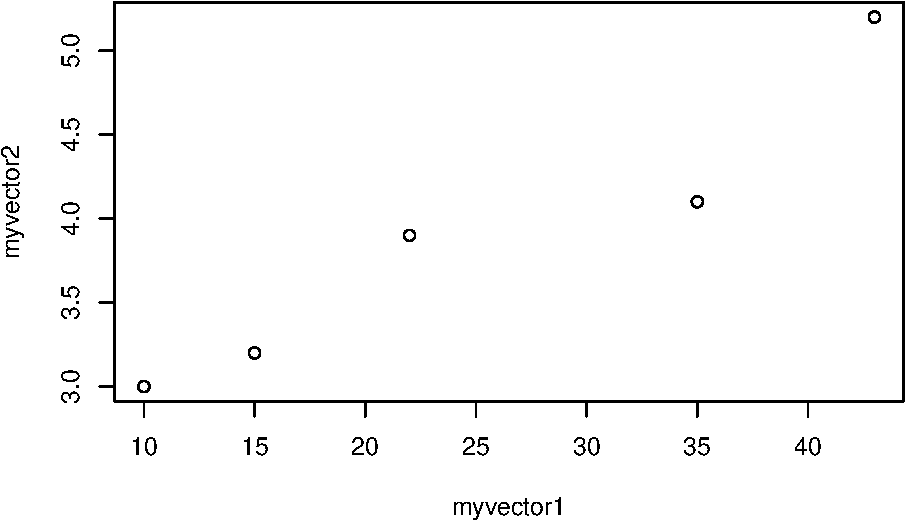
\includegraphics{lbrb_files/figure-latex/unnamed-chunk-152-1.pdf}

If you want to label the axes on the plot, you can do this by giving the plot() function values for its optional arguments xlab and ylab:

\begin{Shaded}
\begin{Highlighting}[]
\FunctionTok{plot}\NormalTok{(myvector1, }
\NormalTok{     myvector2, }
     \AttributeTok{xlab=}\StringTok{"vector1"}\NormalTok{, }
     \AttributeTok{ylab=}\StringTok{"vector2"}\NormalTok{)}
\end{Highlighting}
\end{Shaded}

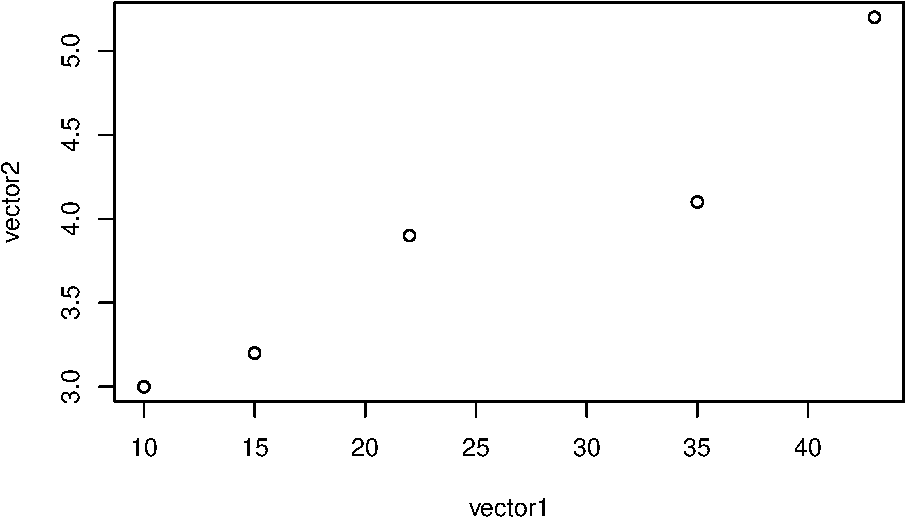
\includegraphics{lbrb_files/figure-latex/unnamed-chunk-153-1.pdf}

We can store character data in vectors so if we want we could do this to set up our labels:

\begin{Shaded}
\begin{Highlighting}[]
\NormalTok{mylabels }\OtherTok{\textless{}{-}}  \FunctionTok{c}\NormalTok{(}\StringTok{"vector1"}\NormalTok{,}\StringTok{"vector2"}\NormalTok{)}
\end{Highlighting}
\end{Shaded}

Then use bracket notation to call the labels from nthe vector

\begin{Shaded}
\begin{Highlighting}[]
\FunctionTok{plot}\NormalTok{(myvector1, }
\NormalTok{     myvector2, }
     \AttributeTok{xlab=}\NormalTok{mylabels[}\DecValTok{1}\NormalTok{],}
     \AttributeTok{ylab=}\NormalTok{mylabels[}\DecValTok{1}\NormalTok{])}
\end{Highlighting}
\end{Shaded}

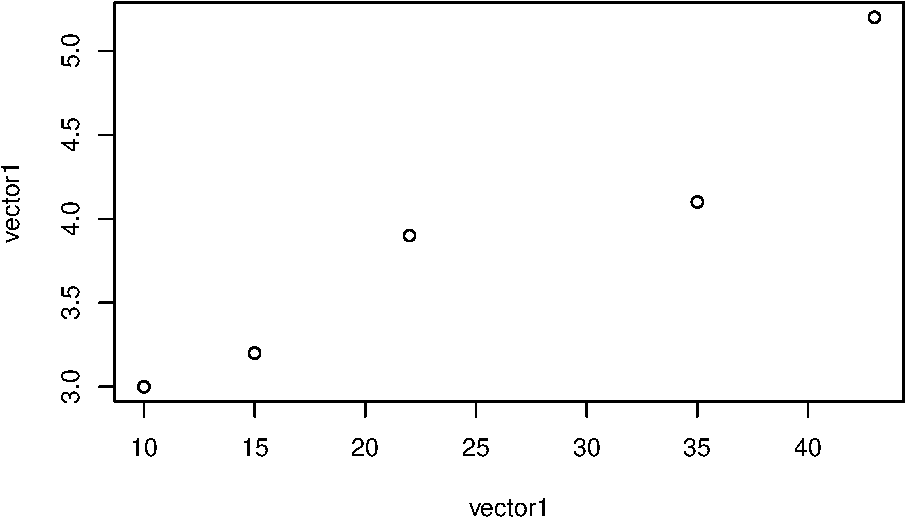
\includegraphics{lbrb_files/figure-latex/unnamed-chunk-155-1.pdf}

The above plot has an error: I intentionlly made it so that ``vector1'' is printed on both axes. In the chunk below make it so that ``vector2'' is printed on the y axis.

\begin{Shaded}
\begin{Highlighting}[]
\FunctionTok{plot}\NormalTok{(myvector1, }
\NormalTok{     myvector2, }
     \AttributeTok{xlab=}\NormalTok{mylabels[}\DecValTok{1}\NormalTok{],}
     \AttributeTok{ylab=}\NormalTok{mylabels[}\DecValTok{1}\NormalTok{])}
\end{Highlighting}
\end{Shaded}

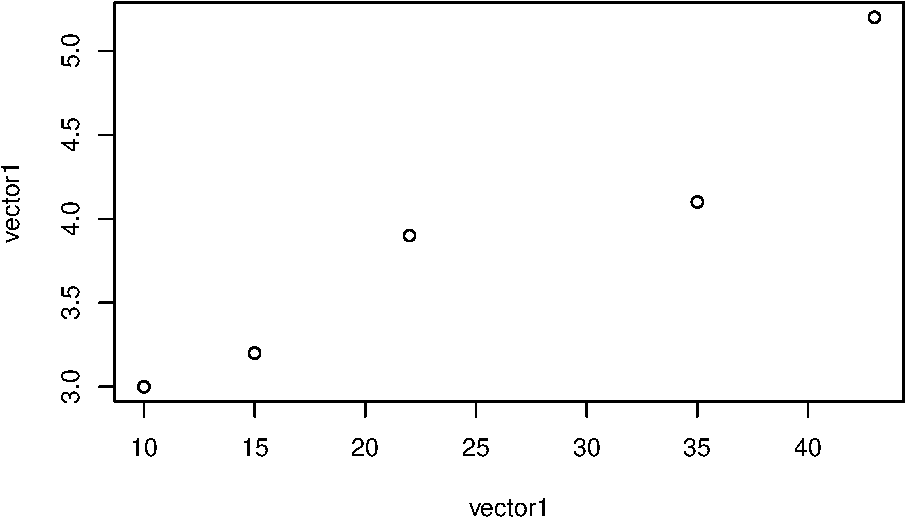
\includegraphics{lbrb_files/figure-latex/unnamed-chunk-156-1.pdf}

Base R has lots of plotting functions; additionally, people have written packages to implement new plotting capabilities. ggplot2 is currently the most popular plotting package, and ggpubr is a package which makes ggplot2 easier to use. For quick plots we'll use base R functions, and when we get to more important things we'll use ggplot2 and ggpubr.

\hypertarget{note-please-save-this-file-with-a-new-file-name-to-your-documents-folder-or-desktop}{%
\chapter{NOTE: please save this file with a new file name to your documents folder or desktop}\label{note-please-save-this-file-with-a-new-file-name-to-your-documents-folder-or-desktop}}

\hypertarget{downloading-sequences-from-uniprot-by-hand}{%
\chapter{Downloading sequences from UniProt by hand}\label{downloading-sequences-from-uniprot-by-hand}}

\begin{Shaded}
\begin{Highlighting}[]
\FunctionTok{library}\NormalTok{(compbio4all)}
\end{Highlighting}
\end{Shaded}

\textbf{By}: Avril Coghlan.

\textbf{Adapted, edited and expanded}: Nathan Brouwer under the Creative Commons 3.0 Attribution License \href{https://creativecommons.org/licenses/by/3.0/}{(CC BY 3.0)}.

TODO / NOTES:

\begin{itemize}
\tightlist
\item
  The original online version has images, though they are somewhat outdated.
\end{itemize}

\hypertarget{vocab-1}{%
\section{Vocab}\label{vocab-1}}

\begin{itemize}
\tightlist
\item
  RefSeq
\item
  manual curation
\item
  UniProt
\item
  accession
\end{itemize}

\hypertarget{uniprot}{%
\section{UniProt}\label{uniprot}}

In a previous vignette you learnt how to retrieve sequences from the NCBI database. The NCBI database is a key database in bioinformatics because it contains essentially all DNA sequences ever sequenced.

As mentioned previously, a subsection of the NCBI database called \textbf{RefSeq} consists of high quality DNA and protein sequence data. Furthermore, the NCBI entries for the RefSeq sequences have been \textbf{manually curated}, which means that expert biologists employed by NCBI have added additional information to the NCBI entries for those sequences, such as details of scientific papers that describe the sequences.

Another extremely important manually curated database is \href{www.uniprot.org}{\textbf{UniProt}}, which focuses on protein sequences. UniProt aims to contains manually curated information on all known protein sequences. While many of the protein sequences in UniProt are also present in RefSeq, the amount and quality of manually curated information in UniProt is much higher than that in RefSeq.

For each protein in UniProt, the UniProt curators read all the scientific papers that they can find about that protein, and add information from those papers to the protein's UniProt entry. For example, for a human protein, the UniProt entry for the protein usually includes information about the biological function of the protein, in what human tissues it is expressed, whether it interacts with other human proteins, and much more. All this information has been manually gathered by the UniProt curators from scientific papers, and the papers in which the found the information are always listed in the UniProt entry for the protein.

Just like NCBI, UniProt also assigns an \textbf{accession} to each sequence in the UniProt database. Although the same protein sequence may appear in both the NCBI database and the UniProt database, it will have \emph{different} NCBI and UniProt accessions. However, there is usually a link on the NCBI entry for the protein sequence to the UniProt entry, and vice versa.

\hypertarget{viewing-the-uniprot-webpage-for-a-protein-sequence}{%
\section{Viewing the UniProt webpage for a protein sequence}\label{viewing-the-uniprot-webpage-for-a-protein-sequence}}

If you are given the UniProt accession for a protein, to find the UniProt entry for the protein, you first need to go the UniProt website, www.uniprot.org. At the top of the UniProt website, you will see a search box, and you can type the accession of the protein that you are looking for in this search box, and then click on the ``Search'' button to search for it.

For example, if you want to find the sequence for the chorismate lyase protein from \emph{Mycobacterium leprae} (the bacterium which causes leprosy), which has UniProt accession Q9CD83, you would type just ``Q9CD83'' in the search box and press ``Search''. The UniProt entry for UniProt accession Q9CD83 will then appear in your web browser.

Beside the heading ``Organism'' you can see the organism is given as \emph{Mycobacterium leprae}. If you scroll down you'll find a section \textbf{Names and Taxonomy} and beside the heading ``Taxonomic lineage'', you can see ``Bacteria - Actinobacteria - Actinobacteridae - Actinomycetales - Corynebacterineae - Mycobacteriaceae- Mycobacterium''.

This tells us that \emph{Mycobacterium} is a species of bacteria, which belongs to a group of related bacteria called the Mycobacteriaceae, which itself belongs to a larger group of related bacteria called the Corynebacterineae, which itself belongs to an even larger group of related bacteria called the Actinomycetales, which itself belongs to the Actinobacteridae, which itself belongs to a huge group of bacteria called the Actinobacteria.

\hypertarget{protein-function}{%
\subsection{Protein function}\label{protein-function}}

Back up at the top under ``organism'' is says ``Status'', which tells us the \textbf{annotation score} is 2 out of 5, that it is a ``Protein inferred from homology'', which means what we know about it is derived from bioinformatics and computational tools, not lab work.

Beside the heading ``Function'', it says that the function of this protein is that it ``Removes the pyruvyl group from chorismate to provide 4-hydroxybenzoate (4HB)''. This tells us this protein is an enzyme (a protein that increases the rate of a specific biochemical reaction), and tells us what is the particular biochemical reaction that this enzyme is involved in. At the end of this info it says ``By similarity'', which again indicates that what we know about this protein comes from bioinformatics, not lab work.

\hypertarget{protein-sequence-and-size}{%
\subsection{Protein sequence and size}\label{protein-sequence-and-size}}

Under \textbf{Sequence} we see that the sequence length is 210 amino acids long (210 letters long) and has a mass of 24,045 daltons. We can access the sequence as a FASTA file from here if we want and also carry out a BLAST search from a link on the right.

\hypertarget{other-information}{%
\subsection{Other information}\label{other-information}}

Further down the UniProt page for this protein, you will see a lot more information, as well as many links to webpages in other biological databases, such as NCBI. The huge amount of information about proteins in UniProt means that if you want to find out about a particular protein, the UniProt page for that protein is a great place to start.

\hypertarget{retrieving-a-uniprot-protein-sequence-via-the-uniprot-website}{%
\section{Retrieving a UniProt protein sequence via the UniProt website}\label{retrieving-a-uniprot-protein-sequence-via-the-uniprot-website}}

There are a couple different ways to retrieve the sequence. At the top of the page is a tab that say ``Format'' which brings you to a page with th FASTA file. You can copy and paste the sequence from here if you want. To save it as a file, go to the ``File'' menu of your web browser, choose ``Save page as'', and save the file. Remember to give the file a sensible name (eg. ``Q9CD83.fasta'' for accession Q9CD83), and in a place that you will remember (eg. in the ``My Documents'' folder).

For example, you can retrieve the protein sequences for the chorismate lyase protein from \emph{Mycobacterium leprae} (which has UniProt accession Q9CD83) and for the chorismate lyase protein from \emph{Mycobacterium ulcerans} (UniProt accession A0PQ23), and save them as FASTA-format files (eg. ``Q9CD83.fasta'' and ``A0PQ23.fasta'', as described above.

You can also put the UniProt information into an online \textbf{Basket}. If you do this for both Q9CD83 and A0PQ23 you can think click on \textbf{Basket}, select both entries, and carry out a pairwise alignment by clicking on \textbf{Align}.

\emph{Mycobacterium leprae} is the bacterium which causes leprosy, while \emph{Mycobacterium ulcerans} is a related bacterium which causes Buruli ulcer, both of which are classified by the WHO as neglected tropical diseases. The \emph{M. leprae} and \emph{M. ulcerans} chorismate lyase proteins are an example of a pair of \textbf{homologous} (related) proteins in two related species of bacteria.

If you downloaded the protein sequences for UniProt accessions Q9CD83 and A0PQ23 and saved them as FASTA-format files (eg. ``Q9CD83.fasta'' and ``A0PQ23.fasta''), you could read them into R using the read.fasta() function in the SeqinR R package (as detailed in another Vignette) or a similar function from another package.

Note that the read.fasta() function normally expects that you have put your FASTA-format files in the the \textbf{working directory} of R. For convenience so you can explore these sequences they have been saved in a special folder in the \emph{dayoff} package and can be accessed like this for the Leprosy sequence

\begin{Shaded}
\begin{Highlighting}[]
\CommentTok{\# load dayoff}
\FunctionTok{library}\NormalTok{(dayoff)}

\CommentTok{\# locate the file within the package using system.file()}
\NormalTok{file}\FloatTok{.1} \OtherTok{\textless{}{-}} \FunctionTok{system.file}\NormalTok{(}\StringTok{"./extdata/Q9CD83.fasta"}\NormalTok{,}\AttributeTok{package =} \StringTok{"dayoff"}\NormalTok{)}

\CommentTok{\# load seqinr}
\FunctionTok{library}\NormalTok{(}\StringTok{"seqinr"}\NormalTok{)}

\CommentTok{\# load fasta}
\NormalTok{leprae }\OtherTok{\textless{}{-}} \FunctionTok{read.fasta}\NormalTok{(}\AttributeTok{file =}\NormalTok{ file}\FloatTok{.1}\NormalTok{)}
\NormalTok{lepraeseq }\OtherTok{\textless{}{-}}\NormalTok{ leprae[[}\DecValTok{1}\NormalTok{]]}
\end{Highlighting}
\end{Shaded}

We can confirm

\begin{Shaded}
\begin{Highlighting}[]
\FunctionTok{str}\NormalTok{(lepraeseq)}
\end{Highlighting}
\end{Shaded}

For the other sequence

\begin{Shaded}
\begin{Highlighting}[]
\CommentTok{\# locate the file within the package using system.file()}
\NormalTok{file}\FloatTok{.1} \OtherTok{\textless{}{-}} \FunctionTok{system.file}\NormalTok{(}\StringTok{"./extdata/A0PQ23.fasta"}\NormalTok{,}\AttributeTok{package =} \StringTok{"dayoff"}\NormalTok{)}


\CommentTok{\# load fasta}
\NormalTok{ulcerans }\OtherTok{\textless{}{-}} \FunctionTok{read.fasta}\NormalTok{(}\AttributeTok{file =} \StringTok{"A0PQ23.fasta"}\NormalTok{)}
\NormalTok{ulceransseq }\OtherTok{\textless{}{-}}\NormalTok{ ulcerans[[}\DecValTok{1}\NormalTok{]]}
\end{Highlighting}
\end{Shaded}

\hypertarget{sequence-databases}{%
\chapter{Sequence Databases}\label{sequence-databases}}

\begin{Shaded}
\begin{Highlighting}[]
\FunctionTok{library}\NormalTok{(compbio4all)}
\end{Highlighting}
\end{Shaded}

\textbf{By}: Avril Coghlan.

\textbf{Adapted, edited and expanded}: Nathan Brouwer under the Creative Commons 3.0 Attribution License \href{https://creativecommons.org/licenses/by/3.0/}{(CC BY 3.0)}.

\hypertarget{querying-the-ncbi-database-via-r}{%
\section{Querying the NCBI Database via R}\label{querying-the-ncbi-database-via-r}}

Instead of carrying out searches of the NCBI database on the NCBI website, you can carry out searches directly from R by using the SeqinR R package.

It is possible to use the SeqinR R package to retrieve sequences from these databases. The SeqinR package was written by the group that created the ACNUC database in Lyon, France (\url{http://pbil.univ-lyon1.fr/databases/acnuc/acnuc.html}). The ACNUC database is a database that contains most of the data from the NCBI Sequence Database, as well as data from other sequence databases such as UniProt and Ensembl.

An advantage of the ACNUC database is that it brings together data from various different sources, and makes it easy to search, for example, by using the SeqinR R package.

As will be explained below, the ACNUC database is organised into various different ACNUC (sub)-databases, which contain different parts of the NCBI database, and when you want to search the NCBI database via R, you will need to specify which ACNUC sub-database the NCBI data that you want to query is stored in.

To obtain a full list of the ACNUC sub-databases that you can access using SeqinR, you can use the ``choosebank()'' function from SeqinR:

\begin{Shaded}
\begin{Highlighting}[]
\FunctionTok{library}\NormalTok{(}\StringTok{"seqinr"}\NormalTok{) }\CommentTok{\# Load the SeqinR R package}
\FunctionTok{choosebank}\NormalTok{()      }\CommentTok{\# List all the sub{-}databases in ACNUC}
\end{Highlighting}
\end{Shaded}

Alas, the ACNUC sub-databases do not have a one-to-one correspondence with the NCBI sub-databases (the NCBI Protein database, NCBI EST database, NCBI Genome database, etc.)!

Three of the most important sub-databases in ACNUC which can be searched from R are:

``genbank'': this contains DNA and RNA sequences from the NCBI Sequence Database, except for certain classes of sequences (eg. draft genome sequence data from genome sequencing projects)
``refseq'': this contains DNA and RNA sequences from Refseq, the curated part of the NCBI Sequence Database
``refseqViruses'': this contains DNA, RNA and proteins sequences from viruses from RefSeq
You can find more information about what each of these ACNUC databases contains by looking at the ACNUC website.

You can carry out complex queries using the ``query()'' function from the SeqinR package. If you look at the help page for the query() function (by typing ``help(query)'', you will see that it allows you to specify criteria that you require the sequences to fulfill.

For example, to search for a sequence with a particular NCBI accession, you can use the ``AC='' argument in ``query()''. The ``query()'' function will then search for sequences in the NCBI Sequence Database that match your criteria.

Just as you can use ``AC='' to specify an accession in a search, you can specify that you want to find sequences whose NCBI records contain a certain keywords by using ``K='' as an argument (input) to the ``query()'' function. Likewise you can limit a search to either DNA or mRNA sequences by using the ``M='' argument for the ``query()'' function. Here are some more possible arguments you can use in the ``query()'' function:

Argument Example Restricts your search to sequences:
``AC='' ``AC=NC\_001477'' With a particular accession number
``SP='' ``SP=Chlamydia'' From a particular organism or taxon
``M='' ``M=mRNA'' Of a specific type (eg. mRNA)
``J='' ``J=Nature'' Described in a paper published in a particular journal
``R='' ``R=Nature/460/352'' Described in a paper in a particular journal, volume and start-page
``AU='' ``AU=Smith'' Described in a paper, or submitted to NCBI, by a particular author
The full list of possible arguments for the ``query()'' funtion are given on its help page. Here are some examples using the query function:

Input to the query() function Searches for sequences:
``AC=NC\_001477'' With accession number NC\_001477
``R=Nature/460/352'' Published in Nature 460:352-358
``SP=Chlamydia trachomatis'' From the bacterium Chlamydia trachomatis
``AU=Berriman'' Published in a paper, or submitted to NCBI, by someone called Berriman
``K=flagellin OR K=fibrinogen'' Which have the keyword `flagellin' or `fibrinogen'
``SP=Mycobacterium leprae AND K=dnaA'' Which are from M. leprae, and have the keyword ``dnaA''
``SP=Homo sapiens AND K=colon cancer'' Which are from human, and have the keyword ``colon cancer''
``SP=Homo sapiens AND K=malaria'' Which are from human, and have the keyword ``malaria''
``SP=Homo sapiens AND M=mrna'' Which are mRNA sequences from human
``SP=Bacteria'' Which are sequences from Bacteria
As explained above, the ACNUC database contains the NCBI sequence data organised into several sub-databases, and you can view the list of those sub-databases by using the ``choosebank()'' function from the SeqinR package. When you want to use ``query()'' to carry out a particular sub-database (eg. ``genbank'', which contains DNA and RNA sequences from the NCBI Sequence Database), you need to first specify the database that you want to search by using the ``choosebank()'' function, for example:

\begin{Shaded}
\begin{Highlighting}[]
\FunctionTok{choosebank}\NormalTok{(}\StringTok{"genbank"}\NormalTok{) }\CommentTok{\# Specify that we want to search the \textquotesingle{}genbank\textquotesingle{} ACNUC sub{-}database}
\end{Highlighting}
\end{Shaded}

Likewise, to specify that we want to search the `refseq' ACNUC sub-database, which contains sequences from the NCBI RefSeq database, we would type:

\begin{Shaded}
\begin{Highlighting}[]
\FunctionTok{choosebank}\NormalTok{(}\StringTok{"refseq"}\NormalTok{) }\CommentTok{\# Specify that we want to search the \textquotesingle{}refseq\textquotesingle{} ACNUC sub{-}database}
\end{Highlighting}
\end{Shaded}

Once you have specified which ACNUC sub-database you want to search, you can carry out a search of that sub-database by using the ``query()'' function. You need to pass the ``query()'' function both a name for your query (which you can make up), and the query itself (which will be in the format of the examples in the table above). For example, if we want to search for RefSeq sequences from Bacteria, we might decide to call our query ``RefSeqBact'', and we would call the ``query()'' function as follows:

\begin{Shaded}
\begin{Highlighting}[]
\FunctionTok{query}\NormalTok{(}\StringTok{"RefSeqBact"}\NormalTok{, }\StringTok{"SP=Bacteria"}\NormalTok{)}
\end{Highlighting}
\end{Shaded}

As explained below, the results of the search are stored in a list variable called ``RefSeqBact'', and can be retrieved from that list variable. The last thing to do once you have completed your search is to close the connection to the ACNUC sub-database that you were searching, by typing:

\begin{Shaded}
\begin{Highlighting}[]
\FunctionTok{closebank}\NormalTok{()}
\end{Highlighting}
\end{Shaded}

Thus, there are three steps involved in carrying out a query using SeqinR: first use ``choosebank()'' to select the ACNUC sub-database to search, secondly use ``query()'' to query the database, and thirdly use ``closebank()'' to close the connection to the ACNUC sub-database.

Another example could be to search for mRNA sequences from the parasitic worm Schistosoma mansoni in the NCBI Nucleotide database. The appropriate ACNUC sub-database to search is the ``genbank'' ACNUC sub-database. We may decide to call our search ``SchistosomamRNA''. Therefore, to carry out the search, we type in R:

\begin{Shaded}
\begin{Highlighting}[]
\FunctionTok{choosebank}\NormalTok{(}\StringTok{"genbank"}\NormalTok{)}
\FunctionTok{query}\NormalTok{(}\StringTok{"SchistosomamRNA"}\NormalTok{, }\StringTok{"SP=Schistosoma mansoni AND M=mrna"}\NormalTok{)}
\FunctionTok{closebank}\NormalTok{()}
\end{Highlighting}
\end{Shaded}

Example: finding the sequence for the DEN-1 Dengue virus genome
Another example could be to search for the DEN-1 Dengue virus genome sequence, which has accession NC\_001477. This is a viral genome sequence, and so should be in the ACNUC sub-database ``refSeqViruses''. Thus to search for this sequence, calling our search ``Dengue1'', we type in R:

\begin{Shaded}
\begin{Highlighting}[]
\FunctionTok{choosebank}\NormalTok{(}\StringTok{"refseqViruses"}\NormalTok{)}
\FunctionTok{query}\NormalTok{(}\StringTok{"Dengue1"}\NormalTok{, }\StringTok{"AC=NC\_001477"}\NormalTok{)}
\end{Highlighting}
\end{Shaded}

The result of the search is now stored in the list variable Dengue1. Remember that a list is an R object that is like a vector, but can contain elements that are numeric and/or contain characters. In this case, the list Dengue1 contains information on the NCBI records that match the query (ie. information on the NCBI record for accession NC\_001477).

If you look at the help page for ``query()'', the details of the arguments are given under the heading ``Arguments'', and the details of the results (outputs) are given under the heading ``Value''. If you read this now, you will see that it tells us that the result of the ``query()'' function is a list with six different named elements, named ``call'', ``name'', ``nelem'', ``typelist'', ``req'', and ``socket''. The content of each of these six named elements is explained, for example, the ``nelem'' element contains the number of sequences that match the query, and the ``req'' element contains their accession numbers.

In our example, the list object Dengue1 is an output of the ``query()'' function, and so has each of these six named elements, as we can find out by using the ``attributes()'' function, and looking at the named elements listed under the heading ``\$names'':

\begin{Shaded}
\begin{Highlighting}[]
\FunctionTok{attributes}\NormalTok{(Dengue1)}
\end{Highlighting}
\end{Shaded}

As explained in the brief introduction to R, we can retrieve the value for each of the named elements in the list Dengue1 by using ``\$'', followed by the element's name, for example, to get the value of the element named ``nelem'' in the list Dengue1, we type:

\begin{Shaded}
\begin{Highlighting}[]
\NormalTok{Dengue1}\SpecialCharTok{$}\NormalTok{nelem}
\end{Highlighting}
\end{Shaded}

This tells us that there was one sequence in the `refseqViruses' ACNUC database that matched the query. This is what we would expect, as there should only be one sequence corresponding to accession NC\_001477.

To obtain the accession numbers of the sequence found, we can type:

\begin{Shaded}
\begin{Highlighting}[]
\NormalTok{Dengue1}\SpecialCharTok{$}\NormalTok{req}
\end{Highlighting}
\end{Shaded}

As expected, the accession number of the matching sequence is NC\_001477.

When you type ``attributes(Dengue1)'' you can see that there are two headings, ``\$names'', and ``\$class''. As explained above, the named elements of the list variable Dengue1 are listed under the heading ``\$names''. In fact, the headings ``\$names'' and ``\$class'' are two attributes of the list variable Dengue1. We can retrieve the values of the attributes of a variable using the ``attr()'' function. For example, to retrieve the value of the attribute ``\$names'' of Dengue1, we type:

\begin{Shaded}
\begin{Highlighting}[]
\FunctionTok{attr}\NormalTok{(Dengue1, }\StringTok{"names"}\NormalTok{)}
\end{Highlighting}
\end{Shaded}

This gives us the value of the attribute ``\$names'', which contains the the names of the named elements of the list variable Dengue1. Similarly, we can retrieve the value of the a attribute ``\$class'' of Dengue1, we type:

\begin{Shaded}
\begin{Highlighting}[]
\FunctionTok{attr}\NormalTok{(Dengue1, }\StringTok{"class"}\NormalTok{)}
\end{Highlighting}
\end{Shaded}

This tells us that the value of the attribute ``\$class'' is ``qaw''.

The final step in retrieving a genomic DNA sequence is to use the ``getSequence()'' function to tell R to retrieve the sequence data. The command below uses ``getSequence()'' to retrieve the sequence data for the DEN-1 Dengue virus genome, and puts the sequence into a variable dengueseq:

\begin{Shaded}
\begin{Highlighting}[]
\NormalTok{ dengueseq }\OtherTok{\textless{}{-}} \FunctionTok{getSequence}\NormalTok{(Dengue1}\SpecialCharTok{$}\NormalTok{req[[}\DecValTok{1}\NormalTok{]])}
\end{Highlighting}
\end{Shaded}

Note that the input to the getSequence() command is Dengue1\$req{[}{[}1{]}{]}, which contains the name of the NCBI record that the list Dengue1 contains information about.

Once you have retrieved a sequence, you can then print it out. The variable dengueseq is a vector containing the nucleotide sequence. Each element of the vector contains one nucleotide of the sequence. Therefore, we can print out the first 50 nucleotides of the DEN-1 Dengue genome sequence by typing:

\begin{Shaded}
\begin{Highlighting}[]
\NormalTok{dengueseq[}\DecValTok{1}\SpecialCharTok{:}\DecValTok{50}\NormalTok{]}
\end{Highlighting}
\end{Shaded}

Note that dengueseq{[}1:50{]} refers to the elements of the vector dengueseq with indices from 1-50. These elements contain the first 50 nucleotides of the DEN-1 Dengue virus genome sequence.

As well as retrieving the DNA (or RNA or protein) sequence itself, SeqinR can also retrieve all the annotations for the sequence, for example, information on when the sequence was sequenced, who sequenced it, what organism is it from, what paper was it described in, what genes were identified in the sequence, and so on.

Once you have retrieved a sequence using SeqinR, you can retrieved its annotations by using the ``getAnnot()'' function. For example, to view the annotations for the DEN-1 Dengue virus genome sequence, we type:

\begin{Shaded}
\begin{Highlighting}[]
\DocumentationTok{\#\# annots \textless{}{-} getAnnot(Dengue1$req[[1]])}
\end{Highlighting}
\end{Shaded}

This stores the annotations information from the NCBI record for the DEN-1 Dengue virus sequence in a vector variable annots, with one line of the NCBI record in each element of the vector. Therefore, we can print out the first 20 lines of the NCBI record by typing:

\begin{Shaded}
\begin{Highlighting}[]
\NormalTok{annots[}\DecValTok{1}\SpecialCharTok{:}\DecValTok{20}\NormalTok{]}
\end{Highlighting}
\end{Shaded}

The line with ``ORGANISM'' in the left column is the organism field, and usually contains the Latin name for the organism (``Dengue virus 1'' here). The line with ``AUTHORS'' in the left column is the authors field, and contain the names of authors that wrote papers to describe the sequence and/or the names of the people who submitted the sequence to the NCBI Database.

When you have finished your running your query and getting the corresponding sequences and annotations, close the connection to the ACNUC sub-database:

\begin{Shaded}
\begin{Highlighting}[]
\FunctionTok{closebank}\NormalTok{()}
\end{Highlighting}
\end{Shaded}

Example: finding the sequences published in Nature 460:352-358
We described above how to search for the sequences published in Nature 460:352-358, using the NCBI website. A second method is to use the SeqinR R package to search the ACNUC databases (which contain the NCBI sequence data) from R.

If you look at the help page the ``query()'' function, you see that you can query for sequences published in a particular paper using R=refcode, specifying the reference as refcode such as in jcode/volume/page (e.g., JMB/13/5432 or R=Nature/396/133). For the paper Nature 460:352-358, we would need to use the refcode `R=Nature/460/352'.

First we need to specify which of the ACNUC databases we want to search. For example, to specify that we want to search the ``genbank'' ACNUC database, which contains DNA and RNA sequences from the NCBI Nucleotide database, we type:

\begin{Shaded}
\begin{Highlighting}[]
\FunctionTok{choosebank}\NormalTok{(}\StringTok{"genbank"}\NormalTok{) }\CommentTok{\# Specify that we want to search the \textquotesingle{}genbank\textquotesingle{} ACNUC sub{-}database}
\end{Highlighting}
\end{Shaded}

We can then search the `genbank' database for sequences that match a specific set of criteria by using the ``query()'' function. For example, to search for sequences that were published in Nature 460:352-358, we type:

\begin{Shaded}
\begin{Highlighting}[]
\FunctionTok{query}\NormalTok{(}\StringTok{\textquotesingle{}naturepaper\textquotesingle{}}\NormalTok{, }\StringTok{\textquotesingle{}R=Nature/460/352\textquotesingle{}}\NormalTok{)}
\end{Highlighting}
\end{Shaded}

The line above tells R that we want to store the results of the query in an R list variable called naturepaper. To get the value of the element named ``nelem'' in the list naturepaper, we type:

\begin{Shaded}
\begin{Highlighting}[]
\NormalTok{naturepaper}\SpecialCharTok{$}\NormalTok{nelem}
\end{Highlighting}
\end{Shaded}

This tells us that there were 19022 sequences in the `genbank' ACNUC database that matched the query. The `genbank' ACNUC database contains DNA or RNA sequences from the NCBI Nucleotide database. Why don't we get the same number of sequences as found by carrying out the search on the NCBI website (where we found 50890 hits to the NCBI Nucleotide database)? The reason is that the ACNUC `genbank' database does not contain all the sequences in the NCBI Nucleotide database, for example, it does not contain sequences that are in RefSeq or many short DNA sequences from sequencing projects.

To obtain the accession numbers of the first five of the 19022 sequences, we can type:

\begin{Shaded}
\begin{Highlighting}[]
\NormalTok{accessions }\OtherTok{\textless{}{-}}\NormalTok{ naturepaper}\SpecialCharTok{$}\NormalTok{req}
\NormalTok{accessions[}\DecValTok{1}\SpecialCharTok{:}\DecValTok{5}\NormalTok{]}
\end{Highlighting}
\end{Shaded}

This tells us that the NCBI accessions of the first five sequences (of the 19022 DNA or RNA sequences found that were published in Nature 460:352-358) are FN357292, FN357293, FN357294, FN357295, and FN357296.

To retrieve these first five sequences, and print out the first 10 nucleotide bases of each sequence, we use the getSequence() command, typing:

\begin{Shaded}
\begin{Highlighting}[]
\ControlFlowTok{for}\NormalTok{ (i }\ControlFlowTok{in} \DecValTok{1}\SpecialCharTok{:}\DecValTok{5}\NormalTok{)}
\NormalTok{  \{}
\NormalTok{     seqi }\OtherTok{\textless{}{-}} \FunctionTok{getSequence}\NormalTok{(naturepaper}\SpecialCharTok{$}\NormalTok{req[[i]])}
     \FunctionTok{print}\NormalTok{(seqi[}\DecValTok{1}\SpecialCharTok{:}\DecValTok{10}\NormalTok{])}
\NormalTok{  \}}
\end{Highlighting}
\end{Shaded}

Note that the input to the getSequence() command is Dengue1\$req{[}{[}i{]}{]}, which contains the name of i th NCBI record that the list naturepaper contains information about.

Once we have carried out our queries and retrieved the sequences, the final step is to close the connection to the ACNUC sub-database that we searched (``genbank'' here):

\begin{Shaded}
\begin{Highlighting}[]
\FunctionTok{closebank}\NormalTok{()}
\end{Highlighting}
\end{Shaded}

Saving sequence data in a FASTA-format file
Once you have retrieved a sequence, or set of sequences from the NCBI Database, using SeqinR, it is conveninent to save the sequences in a file in FASTA format. This can be done using the ``write.fasta()'' function in the SeqinR package, which was introduced in Chapter 1.

If you look at the help page for the ``write.fasta()'' function, you will see that as input it takes a list of vectors, where each vector contains one DNA, RNA or protein sequence.

For example, if you retrieve the sequences of human tRNAs from the NCBI Database by querying the ACNUC ``genbank'' sub-database, you can save the sequences in a FASTA format file called ``humantRNAs.fasta'' by typing:

\begin{Shaded}
\begin{Highlighting}[]
\FunctionTok{choosebank}\NormalTok{(}\StringTok{"genbank"}\NormalTok{)                             }\CommentTok{\# select the ACNUC sub{-}database to be searched}
\FunctionTok{query}\NormalTok{(}\StringTok{"humtRNAs"}\NormalTok{, }\StringTok{"SP=homo sapiens AND M=TRNA"}\NormalTok{)   }\CommentTok{\# specify the query}
\NormalTok{myseqs }\OtherTok{\textless{}{-}} \FunctionTok{getSequence}\NormalTok{(humtRNAs)                   }\CommentTok{\# get the sequences}
\NormalTok{mynames }\OtherTok{\textless{}{-}} \FunctionTok{getName}\NormalTok{(humtRNAs)                      }\CommentTok{\# get the names of the sequences}
\FunctionTok{write.fasta}\NormalTok{(myseqs, mynames, }\AttributeTok{file.out=}\StringTok{"humantRNAs.fasta"}\NormalTok{)}
\FunctionTok{closebank}\NormalTok{()}
\end{Highlighting}
\end{Shaded}

In the above code, we get the sequences of the human tRNAs using the function ``getSequence()'' from the SeqinR package. We also use a function ``getName()'' from the SeqinR package to get the sequences' names. Then we use the ``write.fasta()'' function to write the sequences to a FASTA file ``humantRNAs.fasta''. The ``write.fasta()'' takes as arguments: the list myseqs containing the sequences, the list mynames containing the names of the sequences, and the name of the output file (``humantRNAs.fasta'' here).

Finding the genome sequence for a particular species
Microbial genomes are generally smaller than eukaryotic genomes (Escherichia coli has about 5 million base pair in its genome, while the human genome is about 3 billion base pairs). Because they are considerably less expensive to sequence, many microbial genome sequencing projects have been completed.

If you don't know the accession number for a genome sequence (eg. for Mycobacterium leprae, the bacterium that causes leprosy), how can you find it out?

The easiest way to do this is to look at the NCBI Genome website, which lists all fully sequenced genomes and gives the accession numbers for the corresponding DNA sequences.

If you didn't know the accession number for the Mycobacterium leprae genome, you could find it on the NCBI Genome website by following these steps:

Go to the NCBI Genome website (\url{http://www.ncbi.nlm.nih.gov/sites/entrez?db=Genome})
On the homepage of the NCBI Genome website, it gives links to the major subdivisions of the Genome database, which include Eukaryota, Prokaryota (Bacteria and Archaea), and Viruses. Click on `Prokaryota', since Mycobacterium leprae is a bacterium. This will bring up a list of all fully sequenced bacterial genomes, with the corresponding accession numbers. Note that more than one genome (from various strains) may have been sequenced for a particular species.
Use `Find' in the `Edit' menu of your web browser to search for `Mycobacterium leprae' on the webpage. You should find that the genomes of several different M. leprae strains have been sequenced. One of these is M. leprae TN, which has accession number NC\_002677.
The list of sequenced genomes on the NCBI Genomes website is not a definitive list; that is, some sequenced genomes may be missing from this list. If you want to find out whether a particular genome has been sequenced, but you don't find it NCBI Genomes website's list, you should search for it by following these steps:

Go to the NCBI website (www.ncbi.nlm.nih.gov).
Select `Genome' from the drop-down list above the search box.
Type the name of the species you are interested in in the search box (eg. ``Mycobacterium leprae''{[}ORGN{]}). Press `Search'.
Note that you could also have found the Mycobacterium leprae genome sequence by searching the NCBI Nucleotide database, as the NCBI Genome database is just a subset of the NCBI Nucleotide database.

How many genomes have been sequenced, or are being sequenced now?
On the NCBI Genome website (\url{http://www.ncbi.nlm.nih.gov/sites/entrez?db=Genome}), the front page gives a link to a list of all sequenced genomes in the groups Eukaryota, Prokaryota (Bacteria and Archaea) and Viruses. If you click on one of these links (eg. Prokaryota), at the top of the page it will give the number of sequenced genomes in that group (eg. number of sequenced prokaryotic genomes). For example, in this screenshot (from January 2011), we see that there were 1409 complete prokaryotic genomes (94 archaeal, 1315 bacterial):

image1

Another useful website that lists genome sequencing projects is the Genomes OnLine Database (GOLD), which lists genomes that have been completely sequenced, or are currently being sequenced. To find the number of complete or ongoing bacterial sequencing projects, follow these steps:

Go to the GOLD website (\url{http://genomesonline.org/}).
Click on the yellow `Enter GOLD' button in the centre of the webpage. On the subsequent page, it will give the number of ongoing bacterial, archaeal and eukaryotic genome sequencing projects.

Click on the `Bacterial Ongoing' link to see the list of ongoing bacterial genome sequencing projects. By default, just the first 100 projects are listed, and the rest are listed on subsequent pages. In one of the columns of the page, this gives the university or institute that the genome was sequenced in. Other columns give the taxonomic information for the organism, and links to the sequence data.
Find the number of published genome sequencing projects. Go back one page, to the page with the `Bacterial Ongoing' link. You will see that this page also lists the number of complete published genomes. To see a list of these genomes, click on `Complete Published'. This will bring up a page that gives the number of published genomes at the top of the page. In one column of the page, this gives the university or institute that the genome was sequenced in.
As explained above, it is possible to identify genome sequence data in the NCBI Genome database. The GOLD database also gives some information about ongoing genome projects. Often, the GOLD database lists some ongoing projects that are not yet present in the NCBI Genome Database, because the sequence data has not yet been submitted to the NCBI Database. If you are interested in finding out how many genomes have been sequenced or are currently being sequenced for a particular species (eg. Mycobacterium leprae), it is a good idea to look at both the NCBI Genome database and at GOLD.

\hypertarget{summary-1}{%
\section{Summary}\label{summary-1}}

In this chapter, you have learnt how to retrieve sequences from the NCBI Sequence database, as well as to find out how many genomes have been sequenced or are currently being sequenced for a particular species.

Links and Further Reading
There is detailed information on how to search the NCBI database on the NCBI Help website at \url{http://www.ncbi.nlm.nih.gov/bookshelf/br.fcgi?book=helpentrez?part=EntrezHelp}.

There is more information about the GOLD database in the paper describing GOLD by Liolios et al, which is available at \url{http://www.ncbi.nlm.nih.gov/pmc/articles/PMC2808860/?tool=pubmed}.

For more in-depth information and more examples on using the SeqinR package for sequence analysis, look at the SeqinR documentation, \url{http://pbil.univ-lyon1.fr/software/seqinr/doc.php?lang=eng}.

There is also a very nice chapter on ``Analyzing Sequences'', which includes examples of using SeqinR for sequence analysis, in the book Applied statistics for bioinformatics using R by Krijnen (available online at cran.r-project.org/doc/contrib/Krijnen-IntroBioInfStatistics.pdf).

\hypertarget{acknowledgements-1}{%
\section{Acknowledgements}\label{acknowledgements-1}}

'
Contact
I will be grateful if you will send me (Avril Coghlan) corrections or suggestions for improvements to my email address \href{mailto:alc@sanger.ac.uk}{\nolinkurl{alc@sanger.ac.uk}}

License
The content in this book is licensed under a Creative Commons Attribution 3.0 License.

Exercises
Answer the following questions. For each question, please record your answer, and what you did/typed to get this answer.

Model answers to the exercises are given in Answers to the exercises on Sequence Databases.

\begin{enumerate}
\def\labelenumi{\arabic{enumi}.}
\tightlist
\item
  What information about the rabies virus sequence (NCBI accession NC\_001542) can you obtain from its annotations in the NCBI Sequence Database?
  What does it say in the DEFINITION and ORGANISM fields of its NCBI record? Note: rabies virus is the virus responsible for rabies, which is classified by the WHO as a neglected tropical disease.
\item
  How many nucleotide sequences are there from the bacterium Chlamydia trachomatis in the NCBI Sequence Database?
  Note: the bacterium Chlamydia trachomatis is responsible for causing trachoma, which is classified by the WHO as a neglected tropical disease.
\item
  How many nucleotide sequences are there from the bacterium Chlamydia trachomatis in the RefSeq part of the NCBI Sequence Database?
\item
  How many nucleotide sequences were submitted to NCBI by Matthew Berriman?
\item
  How many nucleotide sequences from nematode worms are there in the RefSeq Database?
  Note that several parasitic nematode worms cause neglected tropical diseases, including \emph{Brugia malayi} and \emph{Wucheria bancrofti}, which cause lymphatic filariasis; Loa loa, which causes subcutaneous filariasis; Onchocerca volvulus, which causes onchocerciasis; and Necator americanus, which causes soil-transmitted helminthiasis.
\item
  How many nucleotide sequences for collagen genes from nematode worms are there in the NCBI Database?
\item
  How many mRNA sequences for collagen genes from nematode worms are there in the NCBI Database?
\item
  How many protein sequences for collagen proteins from nematode worms are there in the NCBI database?
\item
  What is the accession number for the \emph{Trypanosoma cruzi} genome in NCBI?
  Do you see genome sequences for more than one strain of Trypanosoma cruzi? Note that the Trypanosoma cruzi causes Chagas disease, which is classified as a neglected tropical disease by the WHO.
\item
  How many fully sequenced nematode worm species are represented in the NCBI Genome database?
\end{enumerate}

\hypertarget{local-variation-in-gc-content}{%
\chapter{Local variation in GC content}\label{local-variation-in-gc-content}}

\begin{Shaded}
\begin{Highlighting}[]
\FunctionTok{library}\NormalTok{(compbio4all)}
\end{Highlighting}
\end{Shaded}

\textbf{By}: Avril Coghlan.

\textbf{Adapted, edited and expanded}: Nathan Brouwer under the Creative Commons 3.0 Attribution License \href{https://creativecommons.org/licenses/by/3.0/}{(CC BY 3.0)}.

Preliminaries

\begin{Shaded}
\begin{Highlighting}[]
\FunctionTok{library}\NormalTok{(rentrez)}
\FunctionTok{library}\NormalTok{(seqinr)}
\end{Highlighting}
\end{Shaded}

\hypertarget{note-on-the-biology-in-this-section-1}{%
\subsection{Note on the biology in this section}\label{note-on-the-biology-in-this-section-1}}

Some of the biology in this tutorial appears to be out of date. For example, using variation in GC content to ID horizontal gene transfer is currently considered to be biased. The examples are still good for practicing R skills.

\hypertarget{vocabulary-2}{%
\section{Vocabulary}\label{vocabulary-2}}

\begin{itemize}
\tightlist
\item
  \href{https://en.wikipedia.org/wiki/GC-content}{\textbf{GC content}}
\item
  \href{en.wikipedia.org/wiki/Horizontal_gene_transfer}{\textbf{horizontal transfer}}
\item
  \textbf{local variation} in GC content \ldots{}
\end{itemize}

\hypertarget{reading-sequence-data-with-rentrezentrez_fetch}{%
\section{Reading sequence data with rentrez::entrez\_fetch}\label{reading-sequence-data-with-rentrezentrez_fetch}}

In a previous section you learned how to use to search for and download the sequence data for a given NCBI accession from the NCBI Sequence Database, either via the NCBI website using entrez\_fetch() from the rentrez package.

For example, you could have downloaded the sequence data for a the DEN-1 Dengue virus sequence (NCBI accession NC\_001477), and stored it on a file on your computer (eg. ``dengue\_fasta.fasta'').

\begin{Shaded}
\begin{Highlighting}[]
\NormalTok{dengueseq\_fasta }\OtherTok{\textless{}{-}} \FunctionTok{entrez\_fetch}\NormalTok{(}\AttributeTok{db =} \StringTok{"nucleotide"}\NormalTok{, }
                          \AttributeTok{id =} \StringTok{"NC\_001477"}\NormalTok{, }
                          \AttributeTok{rettype =} \StringTok{"fasta"}\NormalTok{)}
\end{Highlighting}
\end{Shaded}

As noted before, the file gets downloaded in FASTA format, which isn't directly useable in R

\begin{verbatim}
## [1] ">NC_001477.1 Dengue virus 1, complete genome\nAGTTGTTAGTCTACGTGGACCGACAAGAACAGTTTCGAATCGGAAGCTTGCTTAACGTAGTTCTAACAGT\nTTTTTATTAGAGAGCAGATCTCTGATGAACAACCAACGGAAAAAGACGGGTCGACCGTCTTTCAATATGC\nTGAAACGCGCGAGAAACCGCGTGTCAACTGTTTCACAGTTGGCGAAGAGATTCTCAAAAGGAT"
\end{verbatim}

\begin{Shaded}
\begin{Highlighting}[]
\NormalTok{fasta\_cleaner }\OtherTok{\textless{}{-}} \ControlFlowTok{function}\NormalTok{(fasta\_object, }\AttributeTok{parse =} \ConstantTok{TRUE}\NormalTok{)\{}

         \CommentTok{\#header \textless{}{-} gsub("\textbackslash{}\textbackslash{}|","",header)}
         \CommentTok{\#header \textless{}{-} gsub("\textbackslash{}\textbackslash{}+","",header)}
         \CommentTok{\#header \textless{}{-} gsub("\textbackslash{}\textbackslash{}=","",header)}
         \CommentTok{\#header \textless{}{-} gsub("\textbackslash{}\textbackslash{}:","",header)}
         \CommentTok{\#header \textless{}{-} gsub("\textbackslash{}\textbackslash{};","",header)}

         \CommentTok{\#fasta\_object \textless{}{-} gsub("\textbackslash{}\textbackslash{}|","",fasta\_object)}
         \CommentTok{\#fasta\_object \textless{}{-} gsub("\textbackslash{}\textbackslash{}+","",fasta\_object)}
         \CommentTok{\#fasta\_object \textless{}{-} gsub("\textbackslash{}\textbackslash{}=","",fasta\_object)}
         \CommentTok{\#fasta\_object \textless{}{-} gsub("\textbackslash{}\textbackslash{}:","",fasta\_object)}
         \CommentTok{\#fasta\_object \textless{}{-} gsub("\textbackslash{}\textbackslash{};","",fasta\_object)}

         \CommentTok{\#fasta\_object \textless{}{-} gsub(header, "", fasta\_object)}

\NormalTok{        fasta\_object }\OtherTok{\textless{}{-}} \FunctionTok{sub}\NormalTok{(}\StringTok{"\^{}(\textgreater{})(.*?)(}\SpecialCharTok{\textbackslash{}\textbackslash{}}\StringTok{n)(.*)(}\SpecialCharTok{\textbackslash{}\textbackslash{}}\StringTok{n}\SpecialCharTok{\textbackslash{}\textbackslash{}}\StringTok{n)"}\NormalTok{,}\StringTok{"}\SpecialCharTok{\textbackslash{}\textbackslash{}}\StringTok{4"}\NormalTok{,fasta\_object)}
\NormalTok{        fasta\_object }\OtherTok{\textless{}{-}} \FunctionTok{gsub}\NormalTok{(}\StringTok{"}\SpecialCharTok{\textbackslash{}n}\StringTok{"}\NormalTok{, }\StringTok{""}\NormalTok{, fasta\_object)}

         \ControlFlowTok{if}\NormalTok{(parse }\SpecialCharTok{==} \ConstantTok{TRUE}\NormalTok{)\{}
\NormalTok{         fasta\_object }\OtherTok{\textless{}{-}}\NormalTok{ stringr}\SpecialCharTok{::}\FunctionTok{str\_split}\NormalTok{(fasta\_object,}
                                   \AttributeTok{pattern =} \StringTok{""}\NormalTok{,}
                                   \AttributeTok{simplify =} \ConstantTok{FALSE}\NormalTok{)}
\NormalTok{         \}}

         \FunctionTok{return}\NormalTok{(fasta\_object[[}\DecValTok{1}\NormalTok{]])}
\NormalTok{ \}}
\end{Highlighting}
\end{Shaded}

We can convert our FASTA object into a vector using the function fasta\_cleaner()

\begin{Shaded}
\begin{Highlighting}[]
\NormalTok{header. }\OtherTok{\textless{}{-}} \StringTok{"\textgreater{}NC\_001477.1 Dengue virus 1, complete genome"}
\NormalTok{dengueseq\_vector }\OtherTok{\textless{}{-}} \FunctionTok{fasta\_cleaner}\NormalTok{(dengueseq\_fasta)}
\end{Highlighting}
\end{Shaded}

Once you have retrieved a sequence from the NCBI Sequence Database and stored it in a vector variable such as dengueseq\_vector in the example above, it is possible to extract \textbf{subsequence} of the sequence by typing the name of the vector (eg. dengueseq\_vector) followed by the square brackets containing the indices for those nucleotides. For example, to obtain nucleotides 452-535 of the DEN-1 Dengue virus genome, we can type:

\begin{Shaded}
\begin{Highlighting}[]
\NormalTok{dengueseq\_vector[}\DecValTok{452}\SpecialCharTok{:}\DecValTok{535}\NormalTok{]}
\end{Highlighting}
\end{Shaded}

\begin{verbatim}
##  [1] "C" "G" "A" "G" "G" "G" "G" "G" "A" "G" "A" "G" "C" "C" "G" "C" "A" "C" "A"
## [20] "T" "G" "A" "T" "A" "G" "T" "T" "A" "G" "C" "A" "A" "G" "C" "A" "G" "G" "A"
## [39] "A" "A" "G" "A" "G" "G" "A" "A" "A" "A" "T" "C" "A" "C" "T" "T" "T" "T" "G"
## [58] "T" "T" "T" "A" "A" "G" "A" "C" "C" "T" "C" "T" "G" "C" "A" "G" "G" "T" "G"
## [77] "T" "C" "A" "A" "C" "A" "T" "G"
\end{verbatim}

\hypertarget{local-variation-in-gc-content-1}{%
\section{Local variation in GC content}\label{local-variation-in-gc-content-1}}

In a previous section, you learned that to find out the \href{https://en.wikipedia.org/wiki/GC-content}{\textbf{GC content}} of a genome sequence (percentage of nucleotides in a genome sequence that are Gs or Cs), you can use the GC() function in the SeqinR package. For example, to find the GC content of the DEN-1 Dengue virus sequence that we have stored in the vector dengueseq\_vector, we can type:

\begin{Shaded}
\begin{Highlighting}[]
\FunctionTok{GC}\NormalTok{(dengueseq\_vector)}
\end{Highlighting}
\end{Shaded}

\begin{verbatim}
## [1] 0.4666977
\end{verbatim}

The output of the GC() is the fraction of nucleotides in a sequence that are Gs or Cs, so to convert it to a percentage we need to multiply by 100.

\begin{Shaded}
\begin{Highlighting}[]
\FunctionTok{GC}\NormalTok{(dengueseq\_vector)}\SpecialCharTok{*}\DecValTok{100}
\end{Highlighting}
\end{Shaded}

\begin{verbatim}
## [1] 46.66977
\end{verbatim}

Thus, the GC content of the DEN-1 Dengue virus genome is about 0.467 or 46.7\%.

Although the GC content of the whole DEN-1 Dengue virus genome sequence is about 46.7\%, there is probably \textbf{local variation} in GC content within the genome. That is, some regions of the genome sequence may have GC contents quite a bit higher than 46.7\%, while some regions of the genome sequence may have GC contents that are quite a big lower than 46.7\%. Local fluctuations in GC content within the genome sequence can provide different interesting information, for example, they may reveal cases of \href{en.wikipedia.org/wiki/Horizontal_gene_transfer}{\textbf{horizontal transfer}} or reveal biases in mutation.

If a chunk of DNA has moved by horizontal transfer from the genome of a species with low GC content to a species with high GC content, the chunk of horizontally transferred DNA could be detected as a region of unusually low GC content in the high-GC recipient genome.

On the other hand, a region unusually low GC content in an otherwise high-GC content genome could also arise due to biases in mutation in that region of the genome, for example, if mutations from Gs/Cs to Ts/As are more common for some reason in that region of the genome than in the rest of the genome.

\hypertarget{a-sliding-window-analysis-of-gc-content}{%
\section{A sliding window analysis of GC content}\label{a-sliding-window-analysis-of-gc-content}}

In order to study local variation in GC content within a genome sequence, we could calculate the GC content for small chunks of the genome sequence. The DEN-1 Dengue virus genome sequence is 10735 nucleotides long. To study variation in GC content within the genome sequence, we could calculate the GC content of chunks of the DEN-1 Dengue virus genome, for example, for each 2000-nucleotide chunk of the genome sequence:

\begin{Shaded}
\begin{Highlighting}[]
\FunctionTok{GC}\NormalTok{(dengueseq\_vector[}\DecValTok{1}\SpecialCharTok{:}\DecValTok{2000}\NormalTok{])      }\CommentTok{\# Calculate the GC content of nucleotides 1{-}2000 of the Dengue genome}
\end{Highlighting}
\end{Shaded}

\begin{verbatim}
## [1] 0.465
\end{verbatim}

\begin{Shaded}
\begin{Highlighting}[]
\FunctionTok{GC}\NormalTok{(dengueseq\_vector[}\DecValTok{2001}\SpecialCharTok{:}\DecValTok{4000}\NormalTok{])   }\CommentTok{\# Calculate the GC content of nucleotides 2001{-}4000 of the Dengue genome}
\end{Highlighting}
\end{Shaded}

\begin{verbatim}
## [1] 0.4525
\end{verbatim}

From the output of the above calculations, we see that the region of the DEN-1 Dengue virus genome from nucleotides 1-2000 has a GC content of 46.5\%, while the region of the Dengue genome from nucleotides 2001-4000 has a GC content of about 45.3\%. Thus, there seems to be some local variation in GC content within the Dengue genome sequence.

Instead of typing in the commands above to tell R to calculate the GC content for each 2000-nucleotide chunk of the DEN-1 Dengue genome, we can use a for loop to carry out the same calculations, but by typing far fewer commands. That is, we can use a for loop to take each 2000-nucleotide chunk of the DEN-1 Dengue virus genome, and to calculate the GC content of each 2000-nucleotide chunk. Below we will explain the following for loop that has been written for this purpose:

\begin{Shaded}
\begin{Highlighting}[]
\NormalTok{starts }\OtherTok{\textless{}{-}} \FunctionTok{seq}\NormalTok{(}\DecValTok{1}\NormalTok{, }\FunctionTok{length}\NormalTok{(dengueseq\_vector)}\SpecialCharTok{{-}}\DecValTok{2000}\NormalTok{, }\AttributeTok{by =} \DecValTok{2000}\NormalTok{)}
\NormalTok{starts}
\end{Highlighting}
\end{Shaded}

\begin{verbatim}
## [1]    1 2001 4001 6001 8001
\end{verbatim}

\begin{Shaded}
\begin{Highlighting}[]
\NormalTok{ n }\OtherTok{\textless{}{-}} \FunctionTok{length}\NormalTok{(starts)    }\CommentTok{\# Find the length of the vector "starts"}
 \ControlFlowTok{for}\NormalTok{ (i }\ControlFlowTok{in} \DecValTok{1}\SpecialCharTok{:}\NormalTok{n) \{}
\NormalTok{        chunk }\OtherTok{\textless{}{-}}\NormalTok{ dengueseq\_vector[starts[i]}\SpecialCharTok{:}\NormalTok{(starts[i]}\SpecialCharTok{+}\DecValTok{1999}\NormalTok{)]}
\NormalTok{        chunkGC }\OtherTok{\textless{}{-}} \FunctionTok{GC}\NormalTok{(chunk)}
        \FunctionTok{print}\NormalTok{ (chunkGC)}
\NormalTok{     \}}
\end{Highlighting}
\end{Shaded}

\begin{verbatim}
## [1] 0.465
## [1] 0.4525
## [1] 0.4705
## [1] 0.479
## [1] 0.4545
\end{verbatim}

The command ``starts \textless- seq(1, length(dengueseq\_vector)-2000, by = 2000)'' stores the result of the seq() command in the vector starts, which contains the values 1, 2001, 4001, 6001, and 8001.

We set the variable n to be equal to the number of elements in the vector starts, so it will be 5 here, since the vector starts contains the five elements 1, 2001, 4001, 6001 and 8001. The line ``for (i in 1:n)'' means that the counter i will take values of 1-5 in subsequent cycles of the for loop. The for loop above is spread over several lines. However, R will not execute the commands within the for loop until you have typed the final ``\}'' at the end of the for loop and pressed ``Return''.

Each of the three commands within the for loop are carried out in each cycle of the loop. In the first cycle of the loop, i is 1, the vector variable chunk is used to store the region from nucleotides 1-2000 of the Dengue virus sequence, the GC content of that region is calculated and stored in the variable chunkGC, and the value of chunkGC is printed out.

In the second cycle of the loop, i is 2, the vector variable chunk is used to store the region from nucleotides 2001-4000 of the Dengue virus sequence, the GC content of that region is calculated and stored in the variable chunkGC, and the value of chunkGC is printed out. The loop continues until the value of i is 5. In the fifth cycle through the loop, the value of i is 5, and so the GC content of the region from nucleotides 8001-10000 is printed out.

Note that we stop the loop when we are looking at the region from nucleotides 8001-10000, instead of continuing to another cycle of the loop where the region under examiniation would be from nucleotides 10001-12000. The reason for this is because the length of the Dengue virus genome sequence is just 10735 nucleotides, so there is not a full 2000-nucleotide region from nucleotide 10001 to the end of the sequence at nucleotide 10735.

The above analysis of local variation in GC content is what is known as a sliding window analysis of GC content. By calculating the GC content in each 2000-nucleotide chunk of the Dengue virus genome, you are effectively sliding a 2000-nucleotide window along the DNA sequence from start to end, and calculating the GC content in each non-overlapping window (chunk of DNA).

Note that this sliding window analysis of GC content is a slightly simplified version of the method usually carried out by bioinformaticians. In this simplified version, we have calculated the GC content in non-overlapping windows along a DNA sequence. However, it is more usual to calculate GC content in overlapping windows along a sequence, although that makes the code slightly more complicated.

A sliding window plot of GC content
It is common to use the data generated from a sliding window analysis to create a sliding window plot of GC content. To create a sliding window plot of GC content, you plot the local GC content in each window of the genome, versus the nucleotide position of the start of each window. We can create a sliding window plot of GC content by typing:

\begin{Shaded}
\begin{Highlighting}[]
\NormalTok{ starts }\OtherTok{\textless{}{-}} \FunctionTok{seq}\NormalTok{(}\DecValTok{1}\NormalTok{, }\FunctionTok{length}\NormalTok{(dengueseq\_vector)}\SpecialCharTok{{-}}\DecValTok{2000}\NormalTok{, }\AttributeTok{by =} \DecValTok{2000}\NormalTok{)}
\NormalTok{ n }\OtherTok{\textless{}{-}} \FunctionTok{length}\NormalTok{(starts)    }\CommentTok{\# Find the length of the vector "starts"}
\NormalTok{ chunkGCs }\OtherTok{\textless{}{-}} \FunctionTok{numeric}\NormalTok{(n) }\CommentTok{\# Make a vector of the same length as vector "starts", but just containing zeroes}
 \ControlFlowTok{for}\NormalTok{ (i }\ControlFlowTok{in} \DecValTok{1}\SpecialCharTok{:}\NormalTok{n) \{}
\NormalTok{        chunk }\OtherTok{\textless{}{-}}\NormalTok{ dengueseq\_vector[starts[i]}\SpecialCharTok{:}\NormalTok{(starts[i]}\SpecialCharTok{+}\DecValTok{1999}\NormalTok{)]}
\NormalTok{        chunkGC }\OtherTok{\textless{}{-}} \FunctionTok{GC}\NormalTok{(chunk)}
        \FunctionTok{print}\NormalTok{(chunkGC)}
\NormalTok{        chunkGCs[i] }\OtherTok{\textless{}{-}}\NormalTok{ chunkGC}
\NormalTok{     \}}
\end{Highlighting}
\end{Shaded}

\begin{verbatim}
## [1] 0.465
## [1] 0.4525
## [1] 0.4705
## [1] 0.479
## [1] 0.4545
\end{verbatim}

\begin{Shaded}
\begin{Highlighting}[]
 \FunctionTok{plot}\NormalTok{(starts,chunkGCs,}\AttributeTok{type=}\StringTok{"b"}\NormalTok{,}\AttributeTok{xlab=}\StringTok{"Nucleotide start position"}\NormalTok{,}\AttributeTok{ylab=}\StringTok{"GC content"}\NormalTok{)}
\end{Highlighting}
\end{Shaded}

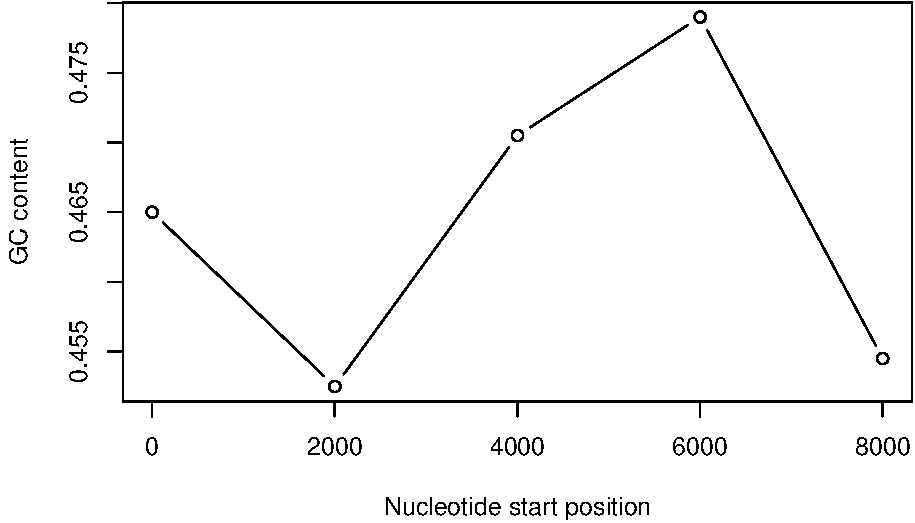
\includegraphics{lbrb_files/figure-latex/unnamed-chunk-201-1.pdf}

In the code above, the line ``chunkGCs \textless- numeric(n)'' makes a new vector chunkGCs which has the same number of elements as the vector starts (5 elements here). This vector chunkGCs is then used within the for loop for storing the GC content of each chunk of DNA.

After the loop, the vector starts can be plotted against the vector chunkGCs using the plot() function, to get a plot of GC content against nucleotide position in the genome sequence. This is a sliding window plot of GC content.

You may want to use the code above to create sliding window plots of GC content of different species' genomes, using different windowsizes. Therefore, it makes sense to write a function to do the sliding window plot, that can take the windowsize that the user wants to use and the sequence that the user wants to study as arguments (inputs):

\begin{Shaded}
\begin{Highlighting}[]
\NormalTok{ slidingwindowplot }\OtherTok{\textless{}{-}} \ControlFlowTok{function}\NormalTok{(windowsize, inputseq)}
\NormalTok{\{}
\NormalTok{   starts }\OtherTok{\textless{}{-}} \FunctionTok{seq}\NormalTok{(}\DecValTok{1}\NormalTok{, }\FunctionTok{length}\NormalTok{(inputseq)}\SpecialCharTok{{-}}\NormalTok{windowsize, }\AttributeTok{by =}\NormalTok{ windowsize)}
\NormalTok{   n }\OtherTok{\textless{}{-}} \FunctionTok{length}\NormalTok{(starts)    }\CommentTok{\# Find the length of the vector "starts"}
\NormalTok{   chunkGCs }\OtherTok{\textless{}{-}} \FunctionTok{numeric}\NormalTok{(n) }\CommentTok{\# Make a vector of the same length as vector "starts", but just containing zeroes}
   \ControlFlowTok{for}\NormalTok{ (i }\ControlFlowTok{in} \DecValTok{1}\SpecialCharTok{:}\NormalTok{n) \{}
\NormalTok{        chunk }\OtherTok{\textless{}{-}}\NormalTok{ inputseq[starts[i]}\SpecialCharTok{:}\NormalTok{(starts[i]}\SpecialCharTok{+}\NormalTok{windowsize}\DecValTok{{-}1}\NormalTok{)]}
\NormalTok{        chunkGC }\OtherTok{\textless{}{-}} \FunctionTok{GC}\NormalTok{(chunk)}
        \FunctionTok{print}\NormalTok{(chunkGC)}
\NormalTok{        chunkGCs[i] }\OtherTok{\textless{}{-}}\NormalTok{ chunkGC}
\NormalTok{   \}}
   \FunctionTok{plot}\NormalTok{(starts,chunkGCs,}\AttributeTok{type=}\StringTok{"b"}\NormalTok{,}\AttributeTok{xlab=}\StringTok{"Nucleotide start position"}\NormalTok{,}\AttributeTok{ylab=}\StringTok{"GC content"}\NormalTok{)}
\NormalTok{\}}
\end{Highlighting}
\end{Shaded}

This function will make a sliding window plot of GC content for a particular input sequence inputseq specified by the user, using a particular windowsize windowsize specified by the user. Once you have typed in this function once, you can use it again and again to make sliding window plots of GC contents for different input DNA sequences, with different windowsizes. For example, you could create two different sliding window plots of the DEN-1 Dengue virus genome sequence, using windowsizes of 3000 and 300 nucleotides, respectively:

\begin{Shaded}
\begin{Highlighting}[]
 \FunctionTok{slidingwindowplot}\NormalTok{(}\DecValTok{3000}\NormalTok{, dengueseq\_vector)}
\end{Highlighting}
\end{Shaded}

\begin{verbatim}
## [1] 0.4646667
## [1] 0.4606667
## [1] 0.4653333
\end{verbatim}

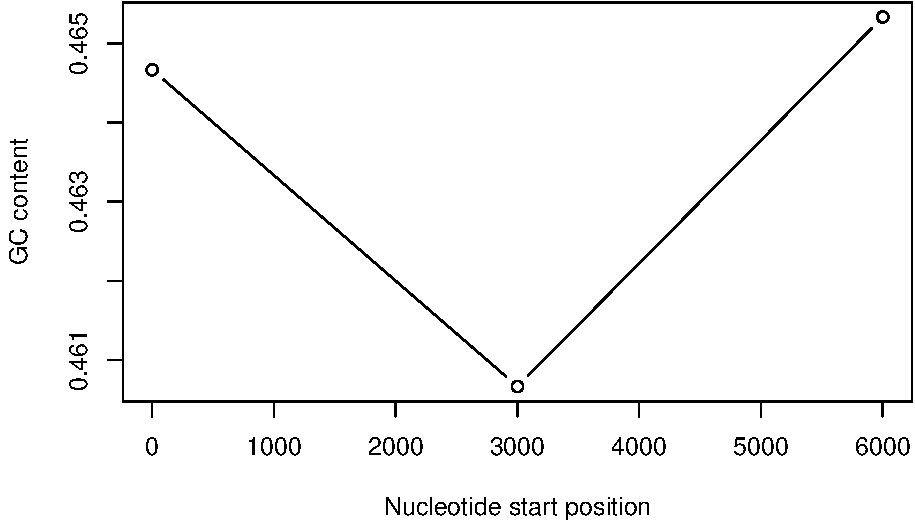
\includegraphics{lbrb_files/figure-latex/unnamed-chunk-203-1.pdf}

\begin{Shaded}
\begin{Highlighting}[]
 \FunctionTok{slidingwindowplot}\NormalTok{(}\DecValTok{300}\NormalTok{, dengueseq\_vector)}
\end{Highlighting}
\end{Shaded}

\begin{verbatim}
## [1] 0.4366667
## [1] 0.4766667
## [1] 0.5
## [1] 0.5066667
## [1] 0.4466667
## [1] 0.4333333
## [1] 0.4466667
## [1] 0.4866667
## [1] 0.4633333
## [1] 0.45
## [1] 0.44
## [1] 0.4633333
## [1] 0.4433333
## [1] 0.4
## [1] 0.4766667
## [1] 0.49
## [1] 0.4733333
## [1] 0.4666667
## [1] 0.4666667
## [1] 0.4866667
## [1] 0.4966667
## [1] 0.48
## [1] 0.49
## [1] 0.49
## [1] 0.4633333
## [1] 0.46
## [1] 0.4633333
## [1] 0.42
## [1] 0.4466667
## [1] 0.4433333
## [1] 0.4466667
## [1] 0.4733333
## [1] 0.4733333
## [1] 0.4966667
## [1] 0.4833333
\end{verbatim}

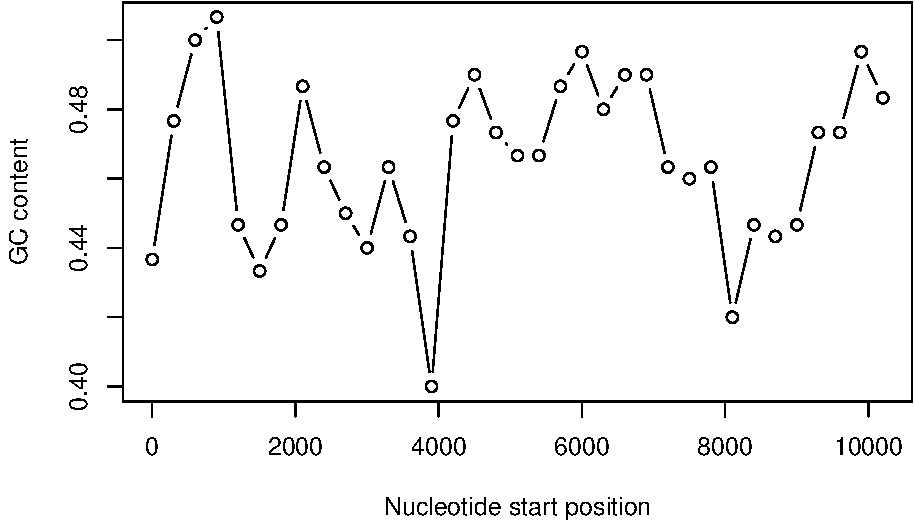
\includegraphics{lbrb_files/figure-latex/unnamed-chunk-204-1.pdf}

\hypertarget{over-represented-and-under-represented-dna-words}{%
\subsection{Over-represented and under-represented DNA words}\label{over-represented-and-under-represented-dna-words}}

In the previous chapter, you learned that the count() function in the SeqinR R package can calculate the frequency of all DNA words of a certain length in a DNA sequence. For example, if you want to know the frequency of all DNA words that are 2 nucleotides long in the Dengue virus genome sequence, you can type:

\begin{Shaded}
\begin{Highlighting}[]
 \FunctionTok{count}\NormalTok{(dengueseq\_vector, }\DecValTok{2}\NormalTok{)}
\end{Highlighting}
\end{Shaded}

\begin{verbatim}
## 
## aa ac ag at ca cc cg ct ga gc gg gt ta tc tg tt 
##  0  0  0  0  0  0  0  0  0  0  0  0  0  0  0  0
\end{verbatim}

It is interesting to identify DNA words that are two nucleotides long (``dinucleotides'', ie. ``AT'', ``AC'', etc.) that are over-represented or under-represented in a DNA sequence. If a particular DNA word is over-represented in a sequence, it means that it occurs many more times in the sequence than you would have expected by chance. Similarly, if a particular DNA word is under-represented in a sequence, it means it occurs far fewer times in the sequence than you would have expected.

A statistic called p (Rho) is used to measure how over- or under-represented a particular DNA word is. For a 2-nucleotide (dinucleotide) DNA word p is calculated as:

p(xy) = fxy/(fx*fy),

where fxy and fx are the frequencies of the DNA words xy and x in the DNA sequence under study. For example, the value of for the DNA word ``TA'' can be calculated as: p(TA) = fTA/(fT* fA), where fTA, fT and fA are the frequencies of the DNA words ``TA'', ``T'' and ``A'' in the DNA sequence.

The idea behind the p statistic is that, if a DNA sequence had a frequency fx of a 1-nucleotide DNA word x, and a frequency fy of a 1-nucleotide DNA word y, then we expect the frequency of the 2-nucleotide DNA word xy to be fx* fy. That is, the frequencies of the 2-nucleotide DNA words in a sequence are expected to be equal the products of the specific frequencies of the two nucleotides that compose them. If this were true, then p would be equal to 1. If we find that p is much greater than 1 for a particular 2-nucleotide word in a sequence, it indicates that that 2-nucleotide word is much more common in that sequence than expected (ie. it is over-represented).

For example, say that your input sequence has only 5\% Ts (ie. fT = 0.05). In a random DNA sequence with 5\% Ts, you would expect to see the word ``TT'' very infrequently. In fact, we would only expect 0.05 * 0.05=0.0025 (0.25\%) of 2-nucleotide words to be TTs (ie. we expect fTT = fT* fT). This is because Ts are rare, so they are expected to be adjacent to each other very infrequently if the few Ts are randomly scattered throughout the DNA. Therefore, if you see lots of TT 2-nucleotide words in your real input sequence (eg. fTT = 0.3, so p = 0.3/0.0025 = 120), you would suspect that natural selection has acted to increase the number of occurrences of the TT word in the sequence (presumably because it has some beneficial biological function).

To find over-represented and under-represented DNA words that are 2 nucleotides long in the DEN-1 Dengue virus sequence, we can calculate the p statistic for each 2-nucleotide word in the sequence. For example, given the number of occurrences of the individual nucleotides A, C, G and T in the Dengue sequence, and the number of occurrences of the DNA word GC in the sequence (500, from above), we can calculate the value of p for the 2-nucleotide DNA word ``GC'', using the formula p(GC) = fGC/(fG * fC), where fGC, fG and fC are the frequencies of the DNA words ``GC'', ``G'' and ``C'' in the DNA sequence:

TODO: is this messed up?

\begin{Shaded}
\begin{Highlighting}[]
\FunctionTok{count}\NormalTok{(dengueseq\_vector, }\DecValTok{1}\NormalTok{) }\CommentTok{\# Get the number of occurrences of 1{-}nucleotide DNA words}
\end{Highlighting}
\end{Shaded}

\begin{verbatim}
## 
## a c g t 
## 0 0 0 0
\end{verbatim}

\begin{Shaded}
\begin{Highlighting}[]
 \DecValTok{2770}\SpecialCharTok{/}\NormalTok{(}\DecValTok{3426}\SpecialCharTok{+}\DecValTok{2240}\SpecialCharTok{+}\DecValTok{2770}\SpecialCharTok{+}\DecValTok{2299}\NormalTok{) }\CommentTok{\# Get fG}
\end{Highlighting}
\end{Shaded}

\begin{verbatim}
## [1] 0.2580345
\end{verbatim}

\begin{Shaded}
\begin{Highlighting}[]
 \DecValTok{2240}\SpecialCharTok{/}\NormalTok{(}\DecValTok{3426}\SpecialCharTok{+}\DecValTok{2240}\SpecialCharTok{+}\DecValTok{2770}\SpecialCharTok{+}\DecValTok{2299}\NormalTok{) }\CommentTok{\# Get fC}
\end{Highlighting}
\end{Shaded}

\begin{verbatim}
## [1] 0.2086633
\end{verbatim}

\begin{Shaded}
\begin{Highlighting}[]
 \FunctionTok{count}\NormalTok{(dengueseq\_vector, }\DecValTok{2}\NormalTok{) }\CommentTok{\# Get the number of occurrences of 2{-}nucleotide DNA words}
\end{Highlighting}
\end{Shaded}

\begin{verbatim}
## 
## aa ac ag at ca cc cg ct ga gc gg gt ta tc tg tt 
##  0  0  0  0  0  0  0  0  0  0  0  0  0  0  0  0
\end{verbatim}

\begin{Shaded}
\begin{Highlighting}[]
\DecValTok{500}\SpecialCharTok{/}\NormalTok{(}\DecValTok{1108}\SpecialCharTok{+}\DecValTok{720}\SpecialCharTok{+}\DecValTok{890}\SpecialCharTok{+}\DecValTok{708}\SpecialCharTok{+}\DecValTok{901}\SpecialCharTok{+}\DecValTok{523}\SpecialCharTok{+}\DecValTok{261}\SpecialCharTok{+}\DecValTok{555}\SpecialCharTok{+}\DecValTok{976}\SpecialCharTok{+}\DecValTok{500}\SpecialCharTok{+}\DecValTok{787}\SpecialCharTok{+}\DecValTok{507}\SpecialCharTok{+}\DecValTok{440}\SpecialCharTok{+}\DecValTok{497}\SpecialCharTok{+}\DecValTok{832}\SpecialCharTok{+}\DecValTok{529}\NormalTok{) }\CommentTok{\# Get fGC}
\end{Highlighting}
\end{Shaded}

\begin{verbatim}
## [1] 0.04658096
\end{verbatim}

\begin{Shaded}
\begin{Highlighting}[]
 \FloatTok{0.04658096}\SpecialCharTok{/}\NormalTok{(}\FloatTok{0.2580345}\SpecialCharTok{*}\FloatTok{0.2086633}\NormalTok{) }\CommentTok{\# Get rho(GC)}
\end{Highlighting}
\end{Shaded}

\begin{verbatim}
## [1] 0.8651364
\end{verbatim}

We calculate a value of p(GC) of approximately 0.865. This means that the DNA word ``GC'' is about 0.865 times as common in the DEN-1 Dengue virus sequence than expected. That is, it seems to be slightly under-represented.

Note that if the ratio of the observed to expected frequency of a particular DNA word is very low or very high, then we would suspect that there is a statistical under-representation or over-representation of that DNA word. However, to be sure that this over- or under-representation is statistically significant, we would need to do a statistical test. We will not deal with the topic of how to carry out the statistical test here.

\hypertarget{summary-2}{%
\section{Summary}\label{summary-2}}

In this chapter, you will have learned to use the following R functions:

seq() for creating a sequence of numbers
print() for printing out the value of a variable
plot() for making a plot (eg. a scatterplot)
numeric() for making a numeric vector of a particular length
function() for making a function
All of these functions belong to the standard installation of R. You also learned how to use for loops to carry out the same operation again and again, each time on different inputs.

\hypertarget{further-reading}{%
\section{Further Reading}\label{further-reading}}

For background reading on DNA sequence statistics, it is recommended to read Chapter 1 of Introduction to Computational Genomics: a case studies approach by Cristianini and Hahn (Cambridge University Press; www.computational-genomics.net/book/).

For more in-depth information and more examples on using the SeqinR package for sequence analysis, look at the SeqinR documentation, \url{http://pbil.univ-lyon1.fr/software/seqinr/doc.php?lang=eng}.

There is also a very nice chapter on ``Analyzing Sequences'', which includes examples of using SeqinR for sequence analysis, in the book Applied statistics for bioinformatics using R by Krijnen (available online at cran.r-project.org/doc/contrib/Krijnen-IntroBioInfStatistics.pdf).

\hypertarget{acknowledgements-2}{%
\section{Acknowledgements}\label{acknowledgements-2}}

This is a modification of \href{https://a-little-book-of-r-for-bioinformatics.readthedocs.io/en/latest/src/chapter1.html}{``DNA Sequence Statistics (1)''} from Avril Coghlan's \href{https://a-little-book-of-r-for-bioinformatics.readthedocs.io/en/latest/index.html}{\emph{A little book of R for bioinformatics.}}. Almost all of text and code was originally written by Dr.~Coghlan and distributed under the \href{https://creativecommons.org/licenses/by/3.0/us/}{Creative Commons 3.0} license.

In ``A little book\ldots{}'' Coghlan write ``Many of the ideas for the examples and exercises for this chapter were inspired by the Matlab case studies on \emph{Haemophilus influenzae} (www.computational-genomics.net/case\_studies/haemophilus\_demo.html) and Bacteriophage lambda (\url{http://www.computational-genomics.net/case_studies/lambdaphage_demo.html}) from the website that accompanies the book Introduction to Computational Genomics: a case studies approach by Cristianini and Hahn (Cambridge University Press; www.computational-genomics.net/book/).''

\hypertarget{license-1}{%
\subsection{License}\label{license-1}}

The content in this book is licensed under a Creative Commons Attribution 3.0 License.

\hypertarget{exercises-1}{%
\section{Exercises}\label{exercises-1}}

Answer the following questions, using the R package. For each question, please record your answer, and what you typed into R to get this answer.

Model answers to the exercises are given in Answers to the exercises on DNA Sequence Statistics (2).

\begin{enumerate}
\def\labelenumi{\arabic{enumi}.}
\tightlist
\item
  Draw a sliding window plot of GC content in the DEN-1 Dengue virus genome, using a window size of 200 nucleotides. Do you see any regions of unusual DNA content in the genome (eg. a high peak or low trough)?
  Make a sketch of each plot that you draw. At what position (in base-pairs) in the genome is there the largest change in local GC content (approximate position is fine here)? Compare the sliding window plots of GC content created using window sizes of 200 and 2000 nucleotides. How does window size affect your ability to detect differences within the Dengue virus genome?
\item
  Draw a sliding window plot of GC content in the genome sequence for the bacterium Mycobacterium leprae strain TN (accession NC\_002677) using a window size of 20000 nucleotides. Do you see any regions of unusual DNA content in the genome (eg. a high peak or low trough)?
\item
  Make a sketch of each plot that you drew for the previous quetion. Write down the approximate nucleotide position of the highest peak or lowest trough that you see. Why do you think a window size of 20000 nucleotides was chosen? What do you see if you use a much smaller windowsize (eg. 200 nucleotides) or a much larger windowsize (eg. 200,000 nucleotides)?
\item
  Advanced: Write a function to calculate the AT content of a DNA sequence (ie. the fraction of the nucleotides in the sequence that are As or Ts). What is the AT content of the Mycobacterium leprae TN genome? Hint: use the function count() to make a table containing the number of As, Gs, Ts and Cs in the sequence. Remember that function count() produces a table object, and you can access the elements of a table object using double square brackets. Do you notice a relationship between the AT content of the \emph{Mycobacterium leprae} TN genome, and its GC content?
\item
  Advanced: Write a function to draw a sliding window plot of AT content. Use it to make a sliding window plot of AT content along the Mycobacterium leprae TN genome, using a windowsize of 20000 nucleotides. Do you notice any relationship between the sliding window plot of GC content along the Mycobacterium leprae genome, and the sliding window plot of AT content? Make a sketch of the plot that you draw.
\item
  Is the 3-nucleotide word GAC GC over-represented or under-represented in the Mycobacterium leprae TN genome sequence? What is the frequency of this word in the sequence? What is the expected frequency of this word in the sequence? What is the p (Rho) value for this word? How would you figure out whether there is already an R function to calculate p (Rho)? Is there one that you could use?
\end{enumerate}

\hypertarget{aligments-in-r}{%
\chapter{Aligments in R}\label{aligments-in-r}}

\begin{Shaded}
\begin{Highlighting}[]
\FunctionTok{library}\NormalTok{(compbio4all)}
\end{Highlighting}
\end{Shaded}

\textbf{By}: Avril Coghlan.

\textbf{Adapted, edited and expanded}: Nathan Brouwer under the Creative Commons 3.0 Attribution License \href{https://creativecommons.org/licenses/by/3.0/}{(CC BY 3.0)}.

\hypertarget{retrieving-a-uniprot-protein-sequence-using-seqinr}{%
\section{Retrieving a UniProt protein sequence using SeqinR}\label{retrieving-a-uniprot-protein-sequence-using-seqinr}}

An alternative method of retrieving a UniProt protein sequence is to use the SeqinR package to query the ACNUC sub-database ``swissprot'', which contains protein sequences from UniProt.

We use the query() function from SeqinR to query this database, as described in chapter3.

For example to retrieve the protein sequences for UniProt accessions Q9CD83 and A0PQ23, we type in R:

\begin{Shaded}
\begin{Highlighting}[]
\NormalTok{leprae\_fasta }\OtherTok{\textless{}{-}}\NormalTok{ rentrez}\SpecialCharTok{::}\FunctionTok{entrez\_fetch}\NormalTok{(}\AttributeTok{db =} \StringTok{"protein"}\NormalTok{,}
                        \AttributeTok{id =} \StringTok{"Q9CD83"}\NormalTok{,}
                         \AttributeTok{rettype =} \StringTok{"fasta"}\NormalTok{)}

\NormalTok{ulcerans\_fasta }\OtherTok{\textless{}{-}}\NormalTok{ rentrez}\SpecialCharTok{::}\FunctionTok{entrez\_fetch}\NormalTok{(}\AttributeTok{db =} \StringTok{"protein"}\NormalTok{,}
                         \AttributeTok{id =} \StringTok{"OIN17619.1"}\NormalTok{,}
                         \AttributeTok{rettype =} \StringTok{"fasta"}\NormalTok{)}
\end{Highlighting}
\end{Shaded}

Display the contents of ``lepraeseq''

\begin{Shaded}
\begin{Highlighting}[]
\NormalTok{leprae\_fasta}
\end{Highlighting}
\end{Shaded}

\begin{verbatim}
## [1] ">sp|Q9CD83.1|PHBS_MYCLE RecName: Full=Chorismate pyruvate-lyase; AltName: Full=4-HB synthase; AltName: Full=p-hydroxybenzoic acid synthase\nMTNRTLSREEIRKLDRDLRILVATNGTLTRVLNVVANEEIVVDIINQQLLDVAPKIPELENLKIGRILQR\nDILLKGQKSGILFVAAESLIVIDLLPTAITTYLTKTHHPIGEIMAASRIETYKEDAQVWIGDLPCWLADY\nGYWDLPKRAVGRRYRIIAGGQPVIITTEYFLRSVFQDTPREELDRCQYSNDIDTRSGDRFVLHGRVFKNL\n\n"
\end{verbatim}

Clean

\begin{Shaded}
\begin{Highlighting}[]
\NormalTok{leprae\_vector }\OtherTok{\textless{}{-}}\FunctionTok{fasta\_cleaner}\NormalTok{(leprae\_fasta)}
\NormalTok{ulcerans\_vector }\OtherTok{\textless{}{-}}\FunctionTok{fasta\_cleaner}\NormalTok{(ulcerans\_fasta)}
\end{Highlighting}
\end{Shaded}

Examine

\begin{Shaded}
\begin{Highlighting}[]
\NormalTok{leprae\_vector}
\end{Highlighting}
\end{Shaded}

\begin{verbatim}
##   [1] "M" "T" "N" "R" "T" "L" "S" "R" "E" "E" "I" "R" "K" "L" "D" "R" "D" "L"
##  [19] "R" "I" "L" "V" "A" "T" "N" "G" "T" "L" "T" "R" "V" "L" "N" "V" "V" "A"
##  [37] "N" "E" "E" "I" "V" "V" "D" "I" "I" "N" "Q" "Q" "L" "L" "D" "V" "A" "P"
##  [55] "K" "I" "P" "E" "L" "E" "N" "L" "K" "I" "G" "R" "I" "L" "Q" "R" "D" "I"
##  [73] "L" "L" "K" "G" "Q" "K" "S" "G" "I" "L" "F" "V" "A" "A" "E" "S" "L" "I"
##  [91] "V" "I" "D" "L" "L" "P" "T" "A" "I" "T" "T" "Y" "L" "T" "K" "T" "H" "H"
## [109] "P" "I" "G" "E" "I" "M" "A" "A" "S" "R" "I" "E" "T" "Y" "K" "E" "D" "A"
## [127] "Q" "V" "W" "I" "G" "D" "L" "P" "C" "W" "L" "A" "D" "Y" "G" "Y" "W" "D"
## [145] "L" "P" "K" "R" "A" "V" "G" "R" "R" "Y" "R" "I" "I" "A" "G" "G" "Q" "P"
## [163] "V" "I" "I" "T" "T" "E" "Y" "F" "L" "R" "S" "V" "F" "Q" "D" "T" "P" "R"
## [181] "E" "E" "L" "D" "R" "C" "Q" "Y" "S" "N" "D" "I" "D" "T" "R" "S" "G" "D"
## [199] "R" "F" "V" "L" "H" "G" "R" "V" "F" "K" "N" "L"
\end{verbatim}

\hypertarget{comparing-two-sequences-using-a-dotplot}{%
\section{Comparing two sequences using a dotplot}\label{comparing-two-sequences-using-a-dotplot}}

As a first step in comparing two protein, RNA or DNA sequences, it is a good idea to make a dotplot. A dotplot is a graphical method that allows the comparison of two protein or DNA sequences and identify regions of close similarity between them. A dotplot is essentially a two-dimensional matrix (like a grid), which has the sequences of the proteins being compared along the vertical and horizontal axes.

In order to make a simple dotplot to represent of the similarity between two sequences, individual cells in the matrix can be shaded black if residues are identical, so that matching sequence segments appear as runs of diagonal lines across the matrix. Identical proteins will have a line exactly on the main diagonal of the dotplot, that spans across the whole matrix.

For proteins that are not identical, but share regions of similarity, the dotplot will have shorter lines that may be on the main diagonal, or off the main diagonal of the matrix. In essence, a dotplot will reveal if there are any regions that are clearly very similar in two protein (or DNA) sequences.

We can create a dotplot for two sequences using the ``dotPlot()'' function in the SeqinR R package.

For example, if we want to create a dotplot of the sequences for the chorismate lyase proteins from Mycobacterium leprae and Mycobacterium ulcerans, we would type:

\begin{Shaded}
\begin{Highlighting}[]
\NormalTok{seqinr}\SpecialCharTok{::}\FunctionTok{dotPlot}\NormalTok{(leprae\_vector, ulcerans\_vector)}
\end{Highlighting}
\end{Shaded}

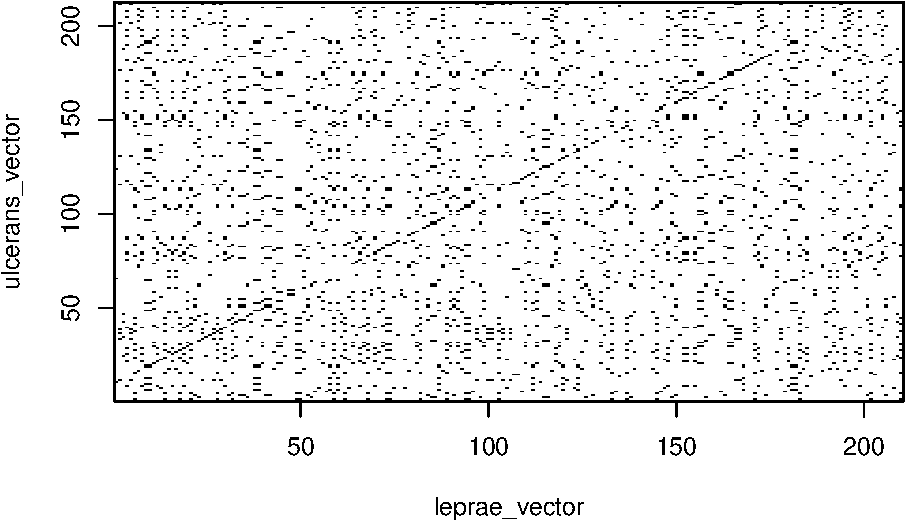
\includegraphics{lbrb_files/figure-latex/unnamed-chunk-217-1.pdf}

In the dotplot above, the \emph{M. leprae} sequence is plotted along the x-axis (horizontal axis), and the \emph{M. ulcerans} sequence is plotted along the y-axis (vertical axis). The dotplot displays a dot at points where there is an identical amino acid in the two sequences.

For example, if amino acid 53 in the \emph{M. leprae} sequence is the same amino acid (eg. ``W'') as amino acid 70 in the M. ulcerans sequence, then the dotplot will show a dot the position in the plot where x =50 and y =53.

In this case you can see a lot of dots along a diagonal line, which indicates that the two protein sequences contain many identical amino acids at the same (or very similar) positions along their lengths. This is what you would expect, because we know that these two proteins are homologues (related proteins).

Pairwise global alignment of DNA sequences using the Needleman-Wunsch algorithm
If you are studying a particular pair of genes or proteins, an important question is to what extent the two sequences are similar.

To quantify similarity, it is necessary to align the two sequences, and then you can calculate a similarity score based on the alignment.

There are two types of alignment in general. A global alignment is an alignment of the full length of two sequences, for example, of two protein sequences or of two DNA sequences. A local alignment is an alignment of part of one sequence to part of another sequence.

The first step in computing a alignment (global or local) is to decide on a scoring system. For example, we may decide to give a score of +2 to a match and a penalty of -1 to a mismatch, and a penalty of -2 to a gap. Thus, for the alignment:

\begin{verbatim}
## [1] "G A A T T C"
\end{verbatim}

\begin{verbatim}
## [1] "G A T T - A"
\end{verbatim}

we would compute a score of 2 + 2 -1 + 2 -2 - 1 = 2.

Similarly, the score for the following alignment is 2 + 2 -2 + 2 + 2 -1 = 5:

\begin{verbatim}
## [1] "G A A T T C"
\end{verbatim}

\begin{verbatim}
## [1] "G A - T T A"
\end{verbatim}

The scoring system above can be represented by a scoring matrix (also known as a substitution matrix). The scoring matrix has one row and one column for each possible letter in our alphabet of letters (eg. 4 rows and 4 columns for DNA sequences). The (i,j) element of the matrix has a value of +2 in case of a match and -1 in case of a mismatch.

We can make a scoring matrix in R by using the nucleotideSubstitutionMatrix() function in the Biostrings() package. The Biostrings package is part of a set of R packages for bioinformatics analysis known as Bioconductor (www.bioconductor.org/).

To use the Biostrings package, you will first need to install the package (see the instructions here).

The arguments (inputs) for the nucleotideSubstitutionMatrix() function are the score that we want to assign to a match and the score that we want to assign to a mismatch. We can also specify that we want to use only the four letters representing the four nucleotides (ie. A, C, G, T) by setting `baseOnly=TRUE', or whether we also want to use the letters that represent ambiguous cases where we are not sure what the nucleotide is (eg. `N' = A/C/G/T).

To make a scoring matrix which assigns a score of +2 to a match and -1 to a mismatch, and store it in the variable sigma, we type:

\begin{Shaded}
\begin{Highlighting}[]
\FunctionTok{library}\NormalTok{(Biostrings)}
\end{Highlighting}
\end{Shaded}

\begin{verbatim}
## Loading required package: BiocGenerics
\end{verbatim}

\begin{verbatim}
## Loading required package: parallel
\end{verbatim}

\begin{verbatim}
## 
## Attaching package: 'BiocGenerics'
\end{verbatim}

\begin{verbatim}
## The following objects are masked from 'package:parallel':
## 
##     clusterApply, clusterApplyLB, clusterCall, clusterEvalQ,
##     clusterExport, clusterMap, parApply, parCapply, parLapply,
##     parLapplyLB, parRapply, parSapply, parSapplyLB
\end{verbatim}

\begin{verbatim}
## The following objects are masked from 'package:stats':
## 
##     IQR, mad, sd, var, xtabs
\end{verbatim}

\begin{verbatim}
## The following objects are masked from 'package:base':
## 
##     anyDuplicated, append, as.data.frame, basename, cbind, colnames,
##     dirname, do.call, duplicated, eval, evalq, Filter, Find, get, grep,
##     grepl, intersect, is.unsorted, lapply, Map, mapply, match, mget,
##     order, paste, pmax, pmax.int, pmin, pmin.int, Position, rank,
##     rbind, Reduce, rownames, sapply, setdiff, sort, table, tapply,
##     union, unique, unsplit, which, which.max, which.min
\end{verbatim}

\begin{verbatim}
## Loading required package: S4Vectors
\end{verbatim}

\begin{verbatim}
## Loading required package: stats4
\end{verbatim}

\begin{verbatim}
## 
## Attaching package: 'S4Vectors'
\end{verbatim}

\begin{verbatim}
## The following object is masked from 'package:base':
## 
##     expand.grid
\end{verbatim}

\begin{verbatim}
## Loading required package: IRanges
\end{verbatim}

\begin{verbatim}
## Loading required package: XVector
\end{verbatim}

\begin{verbatim}
## 
## Attaching package: 'Biostrings'
\end{verbatim}

\begin{verbatim}
## The following object is masked from 'package:seqinr':
## 
##     translate
\end{verbatim}

\begin{verbatim}
## The following object is masked from 'package:base':
## 
##     strsplit
\end{verbatim}

\begin{Shaded}
\begin{Highlighting}[]
\NormalTok{sigma }\OtherTok{\textless{}{-}} \FunctionTok{nucleotideSubstitutionMatrix}\NormalTok{(}\AttributeTok{match =} \DecValTok{2}\NormalTok{, }
                                      \AttributeTok{mismatch =} \SpecialCharTok{{-}}\DecValTok{1}\NormalTok{, }
                                      \AttributeTok{baseOnly =} \ConstantTok{TRUE}\NormalTok{)}
\NormalTok{sigma }\CommentTok{\# Print out the matrix}
\end{Highlighting}
\end{Shaded}

\begin{verbatim}
##    A  C  G  T
## A  2 -1 -1 -1
## C -1  2 -1 -1
## G -1 -1  2 -1
## T -1 -1 -1  2
\end{verbatim}

Instead of assigning the same penalty (eg. -8) to every gap position, it is common instead to assign a gap opening penalty to the first position in a gap (eg. -8), and a smaller gap extension penalty to every subsequent position in the same gap.

The reason for doing this is that it is likely that adjacent gap positions were created by the same insertion or deletion event, rather than by several independent insertion or deletion events. Therefore, we don't want to penalise a 3-letter gap as much as we would penalise three separate 1-letter gaps, as the 3-letter gap may have arisen due to just one insertion or deletion event, while the 3 separate 1-letter gaps probably arose due to three independent insertion or deletion events.

For example, if we want to compute the score for a global alignment of two short DNA sequences `GAATTC' and `GATTA', we can use the Needleman-Wunsch algorithm to calculate the highest-scoring alignment using a particular scoring function.

The ``pairwiseAlignment()'' function in the Biostrings R package finds the score for the optimal global alignment between two sequences using the Needleman-Wunsch algorithm, given a particular scoring system.

As arguments (inputs), the pairwiseAlignment() function takes the two sequences that you want to align, the scoring matrix, the gap opening penalty, and the gap extension penalty. You can also tell the function that you want to just have the optimal global alignment's score by setting ``scoreOnly = TRUE'', or that you want to have both the optimal global alignment and its score by setting ``scoreOnly = FALSE''.

For example, to find the score for the optimal global alignment between the sequences `GAATTC' and `GATTA', we type:

\begin{Shaded}
\begin{Highlighting}[]
\NormalTok{s1 }\OtherTok{\textless{}{-}} \StringTok{"GAATTC"}
\NormalTok{s2 }\OtherTok{\textless{}{-}} \StringTok{"GATTA"}
\end{Highlighting}
\end{Shaded}

\begin{Shaded}
\begin{Highlighting}[]
\NormalTok{globalAligns1s2 }\OtherTok{\textless{}{-}}\NormalTok{ Biostrings}\SpecialCharTok{::}\FunctionTok{pairwiseAlignment}\NormalTok{(s1, s2, }
                                                 \AttributeTok{substitutionMatrix =}\NormalTok{ sigma, }
                                                 \AttributeTok{gapOpening =} \SpecialCharTok{{-}}\DecValTok{2}\NormalTok{,}
                                                 \AttributeTok{gapExtension =} \SpecialCharTok{{-}}\DecValTok{8}\NormalTok{, }
                                                 \AttributeTok{scoreOnly =} \ConstantTok{FALSE}\NormalTok{)}
\end{Highlighting}
\end{Shaded}

\begin{Shaded}
\begin{Highlighting}[]
\NormalTok{globalAligns1s2 }\CommentTok{\# Print out the optimal alignment and its score}
\end{Highlighting}
\end{Shaded}

\begin{verbatim}
## Global PairwiseAlignmentsSingleSubject (1 of 1)
## pattern: GAATTC
## subject: GA-TTA
## score: -3
\end{verbatim}

The above commands print out the optimal global alignment for the two sequences and its score.

Note that we set ``gapOpening'' to be -2 and ``gapExtension'' to be -8, which means that the first position of a gap is assigned a score of (-8-2=)-10, and every subsequent position in a gap is given a score of -8. Here the alignment contains four matches, one mismatch, and one gap of length 1, so its score is (4\emph{2)+(1}-1)+(1*-10) = -3.

Pairwise global alignment of protein sequences using the Needleman-Wunsch algorithm
As well as DNA alignments, it is also possible to make alignments of protein sequences. In this case it is necessary to use a scoring matrix for amino acids rather than for nucleotides.

There are several well known scoring matrices that come with R, such as the BLOSUM series of matrices. Different BLOSUM matrices exist, named with different numbers. BLOSUM with high numbers are designed for comparing closely related sequences, while BLOSUM with low numbers are designed for comparing distantly related sequences. For example, BLOSUM62 is used for less divergent alignments (alignments of sequences that differ little), and BLOSUM30 is used for more divergent alignments (alignments of sequences that differ a lot).

Many R packages come with example data sets or data files. The ``data()'' function is used to load these data files. You can use the data() function in R to load a data set of BLOSUM matrices that comes with R Biostrings() package.

To load the BLOSUM50 matrix, we type:

\begin{Shaded}
\begin{Highlighting}[]
\FunctionTok{data}\NormalTok{(BLOSUM50)}
\NormalTok{BLOSUM50 }\CommentTok{\# Print out the data}
\end{Highlighting}
\end{Shaded}

\begin{verbatim}
##    A  R  N  D  C  Q  E  G  H  I  L  K  M  F  P  S  T  W  Y  V  B  Z  X  *
## A  5 -2 -1 -2 -1 -1 -1  0 -2 -1 -2 -1 -1 -3 -1  1  0 -3 -2  0 -2 -1 -1 -5
## R -2  7 -1 -2 -4  1  0 -3  0 -4 -3  3 -2 -3 -3 -1 -1 -3 -1 -3 -1  0 -1 -5
## N -1 -1  7  2 -2  0  0  0  1 -3 -4  0 -2 -4 -2  1  0 -4 -2 -3  4  0 -1 -5
## D -2 -2  2  8 -4  0  2 -1 -1 -4 -4 -1 -4 -5 -1  0 -1 -5 -3 -4  5  1 -1 -5
## C -1 -4 -2 -4 13 -3 -3 -3 -3 -2 -2 -3 -2 -2 -4 -1 -1 -5 -3 -1 -3 -3 -2 -5
## Q -1  1  0  0 -3  7  2 -2  1 -3 -2  2  0 -4 -1  0 -1 -1 -1 -3  0  4 -1 -5
## E -1  0  0  2 -3  2  6 -3  0 -4 -3  1 -2 -3 -1 -1 -1 -3 -2 -3  1  5 -1 -5
## G  0 -3  0 -1 -3 -2 -3  8 -2 -4 -4 -2 -3 -4 -2  0 -2 -3 -3 -4 -1 -2 -2 -5
## H -2  0  1 -1 -3  1  0 -2 10 -4 -3  0 -1 -1 -2 -1 -2 -3  2 -4  0  0 -1 -5
## I -1 -4 -3 -4 -2 -3 -4 -4 -4  5  2 -3  2  0 -3 -3 -1 -3 -1  4 -4 -3 -1 -5
## L -2 -3 -4 -4 -2 -2 -3 -4 -3  2  5 -3  3  1 -4 -3 -1 -2 -1  1 -4 -3 -1 -5
## K -1  3  0 -1 -3  2  1 -2  0 -3 -3  6 -2 -4 -1  0 -1 -3 -2 -3  0  1 -1 -5
## M -1 -2 -2 -4 -2  0 -2 -3 -1  2  3 -2  7  0 -3 -2 -1 -1  0  1 -3 -1 -1 -5
## F -3 -3 -4 -5 -2 -4 -3 -4 -1  0  1 -4  0  8 -4 -3 -2  1  4 -1 -4 -4 -2 -5
## P -1 -3 -2 -1 -4 -1 -1 -2 -2 -3 -4 -1 -3 -4 10 -1 -1 -4 -3 -3 -2 -1 -2 -5
## S  1 -1  1  0 -1  0 -1  0 -1 -3 -3  0 -2 -3 -1  5  2 -4 -2 -2  0  0 -1 -5
## T  0 -1  0 -1 -1 -1 -1 -2 -2 -1 -1 -1 -1 -2 -1  2  5 -3 -2  0  0 -1  0 -5
## W -3 -3 -4 -5 -5 -1 -3 -3 -3 -3 -2 -3 -1  1 -4 -4 -3 15  2 -3 -5 -2 -3 -5
## Y -2 -1 -2 -3 -3 -1 -2 -3  2 -1 -1 -2  0  4 -3 -2 -2  2  8 -1 -3 -2 -1 -5
## V  0 -3 -3 -4 -1 -3 -3 -4 -4  4  1 -3  1 -1 -3 -2  0 -3 -1  5 -4 -3 -1 -5
## B -2 -1  4  5 -3  0  1 -1  0 -4 -4  0 -3 -4 -2  0  0 -5 -3 -4  5  2 -1 -5
## Z -1  0  0  1 -3  4  5 -2  0 -3 -3  1 -1 -4 -1  0 -1 -2 -2 -3  2  5 -1 -5
## X -1 -1 -1 -1 -2 -1 -1 -2 -1 -1 -1 -1 -1 -2 -2 -1  0 -3 -1 -1 -1 -1 -1 -5
## * -5 -5 -5 -5 -5 -5 -5 -5 -5 -5 -5 -5 -5 -5 -5 -5 -5 -5 -5 -5 -5 -5 -5  1
\end{verbatim}

You can get a list of the available scoring matrices that come with the Biostrings package by using the data() function, which takes as an argument the name of the package for which you want to know the data sets that come with it:

\begin{Shaded}
\begin{Highlighting}[]
\FunctionTok{data}\NormalTok{(}\AttributeTok{package=}\StringTok{"Biostrings"}\NormalTok{)}
\end{Highlighting}
\end{Shaded}

To find the optimal global alignment between the protein sequences ``PAWHEAE'' and ``HEAGAWGHEE'' using the Needleman-Wunsch algorithm using the BLOSUM50 matrix, we type:

\begin{Shaded}
\begin{Highlighting}[]
\FunctionTok{data}\NormalTok{(BLOSUM50)}
\NormalTok{s3 }\OtherTok{\textless{}{-}} \StringTok{"PAWHEAE"}
\NormalTok{s4 }\OtherTok{\textless{}{-}} \StringTok{"HEAGAWGHEE"}
\end{Highlighting}
\end{Shaded}

\begin{Shaded}
\begin{Highlighting}[]
\NormalTok{globalAligns3s4 }\OtherTok{\textless{}{-}} \FunctionTok{pairwiseAlignment}\NormalTok{(s3, s4, }\AttributeTok{substitutionMatrix =} \StringTok{"BLOSUM50"}\NormalTok{, }\AttributeTok{gapOpening =} \SpecialCharTok{{-}}\DecValTok{2}\NormalTok{,}
\AttributeTok{gapExtension =} \SpecialCharTok{{-}}\DecValTok{8}\NormalTok{, }\AttributeTok{scoreOnly =} \ConstantTok{FALSE}\NormalTok{)}
\end{Highlighting}
\end{Shaded}

\begin{Shaded}
\begin{Highlighting}[]
\NormalTok{globalAligns3s4 }\CommentTok{\# Print out the optimal global alignment and its score}
\end{Highlighting}
\end{Shaded}

\begin{verbatim}
## Global PairwiseAlignmentsSingleSubject (1 of 1)
## pattern: P---AWHEAE
## subject: HEAGAWGHEE
## score: -5
\end{verbatim}

We set ``gapOpening'' to be -2 and ``gapExtension'' to be -8, which means that the first position of a gap is assigned a score of (-8-2=)-10, and every subsequent position in a gap is given a score of -8. This means that the gap will be given a score of -10-8-8 = -26.

\hypertarget{aligning-uniprot-sequences}{%
\section{Aligning UniProt sequences}\label{aligning-uniprot-sequences}}

We discussed above how you can search for UniProt accessions and retrieve the corresponding protein sequences, either via the UniProt website or using the SeqinR R package.

In the examples given above, you learned how to retrieve the sequences for the chorismate lyase proteins from Mycobacterium leprae (UniProt Q9CD83) and Mycobacterium ulcerans (UniProt A0PQ23), and read them into R, and store them as vectors lepraeseq and ulceransseq.

You can align these sequences using pairwiseAlignment() from the Biostrings package.

As its input, the pairwiseAlignment() function requires that the sequences be in the form of a single string (eg. ``ACGTA''), rather than as a vector of characters (eg. a vector with the first element as ``A'', the second element as ``C'', etc.). Therefore, to align the M. leprae and M. ulcerans chorismate lyase proteins, we first need to convert the vectors lepraeeq and ulceransseq into strings. We can do this using the c2s() function in the SeqinR package:

\begin{Shaded}
\begin{Highlighting}[]
\NormalTok{lepraeseq\_string }\OtherTok{\textless{}{-}}\NormalTok{ seqinr}\SpecialCharTok{::}\FunctionTok{c2s}\NormalTok{(leprae\_vector)     }\CommentTok{\# Make a string that contains the sequence in "lepraeseq"}
\end{Highlighting}
\end{Shaded}

\begin{Shaded}
\begin{Highlighting}[]
\NormalTok{ulceransseq\_string }\OtherTok{\textless{}{-}}\NormalTok{ seqinr}\SpecialCharTok{::}\FunctionTok{c2s}\NormalTok{(ulcerans\_vector) }\CommentTok{\# Make a string that contains the sequence in "ulceransseq"}
\end{Highlighting}
\end{Shaded}

Furthermore, pairwiseAlignment() requires that the sequences be stored as uppercase characters. Therefore, if they are not already in uppercase, we need to use the toupper() function to convert lepraeseq\_string and ulceransseq\_string to uppercase:

\begin{Shaded}
\begin{Highlighting}[]
\NormalTok{lepraeseq\_string }\OtherTok{\textless{}{-}} \FunctionTok{toupper}\NormalTok{(lepraeseq\_string)}
\NormalTok{ulceransseq\_string }\OtherTok{\textless{}{-}} \FunctionTok{toupper}\NormalTok{(ulceransseq\_string)}
\end{Highlighting}
\end{Shaded}

\begin{Shaded}
\begin{Highlighting}[]
\NormalTok{lepraeseq\_string }\CommentTok{\# Print out the content of "lepraeseq\_string"}
\end{Highlighting}
\end{Shaded}

\begin{verbatim}
## [1] "MTNRTLSREEIRKLDRDLRILVATNGTLTRVLNVVANEEIVVDIINQQLLDVAPKIPELENLKIGRILQRDILLKGQKSGILFVAAESLIVIDLLPTAITTYLTKTHHPIGEIMAASRIETYKEDAQVWIGDLPCWLADYGYWDLPKRAVGRRYRIIAGGQPVIITTEYFLRSVFQDTPREELDRCQYSNDIDTRSGDRFVLHGRVFKNL"
\end{verbatim}

We can now align the the \emph{M. leprae} and \emph{M. ulcerans} chorismate lyase protein sequences using the pairwiseAlignment() function:

\begin{Shaded}
\begin{Highlighting}[]
\NormalTok{globalAlignLepraeUlcerans }\OtherTok{\textless{}{-}}\NormalTok{ Biostrings}\SpecialCharTok{::}\FunctionTok{pairwiseAlignment}\NormalTok{(lepraeseq\_string, }
\NormalTok{                                               ulceransseq\_string,}
                                               \AttributeTok{substitutionMatrix =}\NormalTok{ BLOSUM50, }
                                               \AttributeTok{gapOpening =} \SpecialCharTok{{-}}\DecValTok{2}\NormalTok{, }
                                               \AttributeTok{gapExtension =} \SpecialCharTok{{-}}\DecValTok{8}\NormalTok{, }
                                               \AttributeTok{scoreOnly =} \ConstantTok{FALSE}\NormalTok{)}
\end{Highlighting}
\end{Shaded}

\begin{Shaded}
\begin{Highlighting}[]
\NormalTok{globalAlignLepraeUlcerans }\CommentTok{\# Print out the optimal global alignment and its score}
\end{Highlighting}
\end{Shaded}

\begin{verbatim}
## Global PairwiseAlignmentsSingleSubject (1 of 1)
## pattern: MT-----NR--T---LSREEIRKLDRDLRILVAT...DTPREELDRCQYSNDIDTRSGDRFVLHGRVFKNL
## subject: MLAVLPEKREMTECHLSDEEIRKLNRDLRILIAT...DNSREEPIRHQRS--VGT-SA-R---SGRSICT-
## score: 627
\end{verbatim}

As the alignment is very long, when you type globalAlignLepraeUlcerans, you only see the start and the end of the alignment (see above). Therefore, we need to have a function to print out the whole alignment (see below).

Viewing a long pairwise alignment
If you want to view a long pairwise alignment such as that between the M. leprae and M. ulerans chorismate lyase proteins, it is convenient to print out the alignment in blocks.

The R function ``printPairwiseAlignment()'' below will do this for you:

To use this function you first need to copy and paste this function into R. You can then use our function printPairwiseAlignment() to print out the alignment between the M. leprae and M. ulcerans chorismate lyase proteins (we stored this alignment in the globalAlignLepraeUlcerans variable, see above), in blocks of 60 alignment columns:

\begin{Shaded}
\begin{Highlighting}[]
\FunctionTok{printPairwiseAlignment}\NormalTok{(globalAlignLepraeUlcerans, }\DecValTok{60}\NormalTok{)}
\end{Highlighting}
\end{Shaded}

\begin{verbatim}
## [1] "MT-----NR--T---LSREEIRKLDRDLRILVATNGTLTRVLNVVANEEIVVDIINQQLL 50"
## [1] "MLAVLPEKREMTECHLSDEEIRKLNRDLRILIATNGTLTRILNVLANDEIVVEIVKQQIQ 60"
## [1] " "
## [1] "DVAPKIPELENLKIGRILQRDILLKGQKSGILFVAAESLIVIDLLPTAITTYLTKTHHPI 110"
## [1] "DAAPEMDGCDHSSIGRVLRRDIVLKGRRSGIPFVAAESFIAIDLLPPEIVASLLETHRPI 120"
## [1] " "
## [1] "GEIMAASRIETYKEDAQVWIGDLPCWLADYGYWDLPKRAVGRRYRIIAGGQPVIITTEYF 170"
## [1] "GEVMAASCIETFKEEAKVWAGESPAWLELDRRRNLPPKVVGRQYRVIAEGRPVIIITEYF 180"
## [1] " "
## [1] "LRSVFQDTPREELDRCQYSNDIDTRSGDRFVLHGRVFKN 230"
## [1] "LRSVFEDNSREEPIRHQRS--VGT-SA-R---SGRSICT 233"
## [1] " "
\end{verbatim}

The position in the protein of the amino acid that is at the end of each line of the printed alignment is shown after the end of the line. For example, the first line of the alignment above finishes at amino acid position 50 in the M. leprae protein and also at amino acid position 60 in the M. ulcerans protein.

Since we are printing out an alignment that contained gaps in the first 60 alignment columns, the first 60 alignment columns ends before the 60th amino acid in the M. leprae sequence.

Pairwise local alignment of protein sequences using the Smith-Waterman algorithm
You can use the pairwiseAlignment() function to find the optimal local alignment of two sequences, that is the best alignment of parts (subsequences) of those sequences, by using the ``type=local'' argument in pairwiseAlignment(). This uses the Smith-Waterman algorithm for local alignment, the classic bioinformatics algorithm for finding optimal local alignments.

For example, to find the best local alignment between the M. leprae and M. ulcerans chorismate lyase proteins, we can type:

\begin{Shaded}
\begin{Highlighting}[]
\NormalTok{localAlignLepraeUlcerans }\OtherTok{\textless{}{-}} \FunctionTok{pairwiseAlignment}\NormalTok{(lepraeseq\_string, }
\NormalTok{                                              ulceransseq\_string,}
                                              \AttributeTok{substitutionMatrix =}\NormalTok{ BLOSUM50, }
                                              \AttributeTok{gapOpening =} \SpecialCharTok{{-}}\DecValTok{2}\NormalTok{, }
                                              \AttributeTok{gapExtension =} \SpecialCharTok{{-}}\DecValTok{8}\NormalTok{, }
                                              \AttributeTok{scoreOnly =} \ConstantTok{FALSE}\NormalTok{, }
                                              \AttributeTok{type=}\StringTok{"local"}\NormalTok{)}
\end{Highlighting}
\end{Shaded}

Print out the optimal local alignment and its score

\begin{Shaded}
\begin{Highlighting}[]
\NormalTok{localAlignLepraeUlcerans }
\end{Highlighting}
\end{Shaded}

\begin{verbatim}
## Local PairwiseAlignmentsSingleSubject (1 of 1)
## pattern:  [1] MTNRTLSREEIRKLDRDLRILVATNGTLTRVL...TEYFLRSVFQDTPREELDRCQYSNDIDTRSG
## subject: [11] MTECHLSDEEIRKLNRDLRILIATNGTLTRIL...TEYFLRSVFEDNSREEPIRHQRSVGTSARSG
## score: 761
\end{verbatim}

\begin{Shaded}
\begin{Highlighting}[]
\FunctionTok{printPairwiseAlignment}\NormalTok{(localAlignLepraeUlcerans, }\DecValTok{60}\NormalTok{)}
\end{Highlighting}
\end{Shaded}

\begin{verbatim}
## [1] "MTNRTLSREEIRKLDRDLRILVATNGTLTRVLNVVANEEIVVDIINQQLLDVAPKIPELE 60"
## [1] "MTECHLSDEEIRKLNRDLRILIATNGTLTRILNVLANDEIVVEIVKQQIQDAAPEMDGCD 60"
## [1] " "
## [1] "NLKIGRILQRDILLKGQKSGILFVAAESLIVIDLLPTAITTYLTKTHHPIGEIMAASRIE 120"
## [1] "HSSIGRVLRRDIVLKGRRSGIPFVAAESFIAIDLLPPEIVASLLETHRPIGEVMAASCIE 120"
## [1] " "
## [1] "TYKEDAQVWIGDLPCWLADYGYWDLPKRAVGRRYRIIAGGQPVIITTEYFLRSVFQDTPR 180"
## [1] "TFKEEAKVWAGESPAWLELDRRRNLPPKVVGRQYRVIAEGRPVIIITEYFLRSVFEDNSR 180"
## [1] " "
## [1] "EELDRCQYSNDIDTRSG 240"
## [1] "EEPIRHQRSVGTSARSG 240"
## [1] " "
\end{verbatim}

We see that the optimal local alignment is quite similar to the optimal global alignment in this case, except that it excludes a short region of poorly aligned sequence at the start and at the ends of the two proteins.

\hypertarget{retrieving-multiple-sequences-in-r}{%
\chapter{Retrieving multiple sequences in R}\label{retrieving-multiple-sequences-in-r}}

\begin{Shaded}
\begin{Highlighting}[]
\FunctionTok{library}\NormalTok{(compbio4all)}
\end{Highlighting}
\end{Shaded}

\textbf{By}: Avril Coghlan.\\
Multiple Alignment and Phylogenetic trees
\url{https://a-little-book-of-r-for-bioinformatics.readthedocs.io/en/latest/src/chapter5.html}

\textbf{Adapted, edited and expanded}: Nathan Brouwer under the Creative Commons 3.0 Attribution License \href{https://creativecommons.org/licenses/by/3.0/}{(CC BY 3.0)}.

\hypertarget{prelminaries}{%
\section{Prelminaries}\label{prelminaries}}

\begin{Shaded}
\begin{Highlighting}[]
\FunctionTok{library}\NormalTok{(rentrez)}
\end{Highlighting}
\end{Shaded}

\hypertarget{retrieving-a-list-of-sequences-from-uniprot}{%
\section{Retrieving a list of sequences from UniProt}\label{retrieving-a-list-of-sequences-from-uniprot}}

Using websites or R you can search fort DNA or protein sequences in sequence databases such as the \textbf{NCBI} database and \textbf{UniProt}. Oftentimes, it is useful to retrieve several sequences at once. The R function entrez\_fetch() from the \emph{rentrez} package is useful for this purpose. (Other packages can also, this but \emph{rentrez} has the cleanset interface).

As its input, you need to give the entrez\_fetch() a vector containing the \textbf{accessions} for the sequences you wish to retrieve, as well as the name of the \textbf{ACNUC sub-database} that the sequences should be retrieved from. In this case, we want to retrieve sequences from \textbf{UniProt}, so the sequences should be in the ``swissprot'' ACNUC sub-database. (It can be tricky to know exactly where to get sequences from sometimes so I will usually give you the code to do this).

The entrez\_fetch() function returns a \textbf{list} variable, in which each element is a separate \textbf{vector} containing one of the sequences of interest. **Lists* are a common data structure in R and can take some getting used to, but by working with them we will become familiar with how they work. Unfortunately there are some quirks to have R likes you to write code referring to lists, so I will frequently provide the necessary code for this.

To retrieve the protein sequences for UniProt accessions P06747, P0C569, O56773 and Q5VKP1 (the accessions for rabies virus phosphoprotein, Mokola virus phosphoprotein, Lagos bat virus phosphoprotein and Western Caucasian bat virus phosphoprotein, respectively), you can type:ake a vector containing the names of the sequences. Note that the accessions aren't numbers but are \textbf{quoted character strings}:

\begin{Shaded}
\begin{Highlighting}[]
\NormalTok{seqnames }\OtherTok{\textless{}{-}} \FunctionTok{c}\NormalTok{(}\StringTok{"P06747"}\NormalTok{, }\StringTok{"P0C569"}\NormalTok{, }\StringTok{"O56773"}\NormalTok{, }\StringTok{"Q5VKP1"}\NormalTok{)  }
\end{Highlighting}
\end{Shaded}

Confirm that we are working with character data using is.character()

\begin{Shaded}
\begin{Highlighting}[]
\FunctionTok{is.character}\NormalTok{(seqnames)}
\end{Highlighting}
\end{Shaded}

\begin{verbatim}
## [1] TRUE
\end{verbatim}

We can access the first element of the vector using bracket notation like this:

\begin{Shaded}
\begin{Highlighting}[]
\NormalTok{seqnames[}\DecValTok{1}\NormalTok{]}
\end{Highlighting}
\end{Shaded}

\begin{verbatim}
## [1] "P06747"
\end{verbatim}

Write the code to access the second and third elements of the vector of accessions:

\begin{Shaded}
\begin{Highlighting}[]
\CommentTok{\# 2nd accession}


\CommentTok{\# 3rd accession}
\end{Highlighting}
\end{Shaded}

This code retrieves the first sequence and store them in list variable ``seqs''

\begin{Shaded}
\begin{Highlighting}[]
\NormalTok{seq1 }\OtherTok{\textless{}{-}}\NormalTok{ rentrez}\SpecialCharTok{::}\FunctionTok{entrez\_fetch}\NormalTok{(}\AttributeTok{db =} \StringTok{"protein"}\NormalTok{, }
                          \AttributeTok{id =}\NormalTok{ seqnames[}\DecValTok{1}\NormalTok{], }
                          \AttributeTok{rettype =} \StringTok{"fasta"}\NormalTok{)      }
\end{Highlighting}
\end{Shaded}

\begin{Shaded}
\begin{Highlighting}[]
\NormalTok{seq2 }\OtherTok{\textless{}{-}}\NormalTok{ rentrez}\SpecialCharTok{::}\FunctionTok{entrez\_fetch}\NormalTok{(}\AttributeTok{db =} \StringTok{"protein"}\NormalTok{, }
                          \AttributeTok{id =}\NormalTok{ seqnames[}\DecValTok{2}\NormalTok{], }
                          \AttributeTok{rettype =} \StringTok{"fasta"}\NormalTok{) }

\NormalTok{seq3 }\OtherTok{\textless{}{-}}\NormalTok{ rentrez}\SpecialCharTok{::}\FunctionTok{entrez\_fetch}\NormalTok{(}\AttributeTok{db =} \StringTok{"protein"}\NormalTok{, }
                          \AttributeTok{id =}\NormalTok{ seqnames[}\DecValTok{3}\NormalTok{], }
                          \AttributeTok{rettype =} \StringTok{"fasta"}\NormalTok{)}
\end{Highlighting}
\end{Shaded}

\begin{Shaded}
\begin{Highlighting}[]
\NormalTok{seq1 }\OtherTok{\textless{}{-}} \FunctionTok{fasta\_cleaner}\NormalTok{(seq1, }\AttributeTok{parse =}\NormalTok{ T)  }
\NormalTok{seq2 }\OtherTok{\textless{}{-}} \FunctionTok{fasta\_cleaner}\NormalTok{(seq2, }\AttributeTok{parse =}\NormalTok{ T)  }
\NormalTok{seq3 }\OtherTok{\textless{}{-}} \FunctionTok{fasta\_cleaner}\NormalTok{(seq3, }\AttributeTok{parse =}\NormalTok{ T)  }
\end{Highlighting}
\end{Shaded}

Print out the first 20 letters of the first sequence

\begin{Shaded}
\begin{Highlighting}[]
\NormalTok{seq1[}\DecValTok{1}\SpecialCharTok{:}\DecValTok{20}\NormalTok{]                                   }
\end{Highlighting}
\end{Shaded}

\begin{verbatim}
##  [1] "M" "S" "K" "I" "F" "V" "N" "P" "S" "A" "I" "R" "A" "G" "L" "A" "D" "L" "E"
## [20] "M"
\end{verbatim}

Print out the first 20 letters of the second sequence

\begin{Shaded}
\begin{Highlighting}[]
\NormalTok{seq2[}\DecValTok{1}\SpecialCharTok{:}\DecValTok{20}\NormalTok{]                                   }
\end{Highlighting}
\end{Shaded}

\begin{verbatim}
##  [1] "M" "S" "K" "D" "L" "V" "H" "P" "S" "L" "I" "R" "A" "G" "I" "V" "E" "L" "E"
## [20] "M"
\end{verbatim}

\begin{Shaded}
\begin{Highlighting}[]
\NormalTok{seq\_1\_2\_3\_4 }\OtherTok{\textless{}{-}}\NormalTok{ rentrez}\SpecialCharTok{::}\FunctionTok{entrez\_fetch}\NormalTok{(}\AttributeTok{db =} \StringTok{"protein"}\NormalTok{, }
                          \AttributeTok{id =}\NormalTok{ seqnames, }
                          \AttributeTok{rettype =} \StringTok{"fasta"}\NormalTok{)}
\end{Highlighting}
\end{Shaded}

\begin{Shaded}
\begin{Highlighting}[]
\FunctionTok{cat}\NormalTok{(seq\_1\_2\_3\_4)}
\end{Highlighting}
\end{Shaded}

\begin{verbatim}
## >sp|P06747.1|PHOSP_RABVP RecName: Full=Phosphoprotein; Short=Protein P; AltName: Full=Protein M1
## MSKIFVNPSAIRAGLADLEMAEETVDLINRNIEDNQAHLQGEPIEVDNLPEDMGRLHLDDGKSPNPGEMA
## KVGEGKYREDFQMDEGEDPSLLFQSYLDNVGVQIVRQIRSGERFLKIWSQTVEEIISYVAVNFPNPPGKS
## SEDKSTQTTGRELKKETTPTPSQRESQSSKARMAAQTASGPPALEWSATNEEDDLSVEAEIAHQIAESFS
## KKYKFPSRSSGILLYNFEQLKMNLDDIVKEAKNVPGVTRLARDGSKLPLRCVLGWVALANSKKFQLLVES
## NKLSKIMQDDLNRYTSC
## 
## >sp|P0C569.1|PHOSP_MOKV RecName: Full=Phosphoprotein; Short=Protein P; AltName: Full=Protein M1
## MSKDLVHPSLIRAGIVELEMAEETTDLINRTIESNQAHLQGEPLYVDSLPEDMSRLRIEDKSRRTKTEEE
## ERDEGSSEEDNYLSEGQDPLIPFQNFLDEIGARAVKRLKTGEGFFRVWSALSDDIKGYVSTNIMTSGERD
## TKSIQIQTEPTASVSSGNESRHDSESMHDPNDKKDHTPDHDVVPDIESSTDKGEIRDIEGEVAHQVAESF
## SKKYKFPSRSSGIFLWNFEQLKMNLDDIVKAAMNVPGVERIAEKGGKLPLRCILGFVALDSSKRFRLLAD
## NDKVARLIQEDINSYMARLEEAE
## 
## >sp|O56773.1|PHOSP_LBV RecName: Full=Phosphoprotein; Short=Protein P; AltName: Full=Protein M1
## MSKGLIHPSAIRSGLVDLEMAEETVDLVHKNLADSQAHLQGEPLNVDSLPEDMRKMRLTNAPSEREIIEE
## DEEEYSSEDEYYLSQGQDPMVPFQNFLDELGTQIVRRMKSGDGFFKIWSAASEDIKGYVLSTFMKPETQA
## TVSKPTQTDSLSVPRPSQGYTSVPRDKPSNSESQGGGVKPKKVQKSEWTRDTDEISDIEGEVAHQVAESF
## SKKYKFPSRSSGIFLWNFEQLKMNLDDIVKTSMNVPGVDKIAEKGGKLPLRCILGFVSLDSSKRFRLLAD
## TDKVARLMQDDIHNYMTRIEEIDHN
## 
## >sp|Q5VKP1.1|PHOSP_WCBV RecName: Full=Phosphoprotein; Short=Protein P; AltName: Full=Protein M1
## MSKSLIHPSDLRAGLADIEMADETVDLVYKNLSEGQAHLQGEPFDIKDLPEGVSKLQISDNVRSDTSPNE
## YSDEDDEEGEDEYEEVYDPVSAFQDFLDETGSYLISKLKKGEKIKKTWSEVSRVIYSYVMSNFPPRPPKP
## TTKDIAVQADLKKPNEIQKISEHKSKSEPSPREPVVEMHKHATLENPEDDEGALESEIAHQVAESYSKKY
## KFPSKSSGIFLWNFEQLKMNLDDIVQVARGVPGISQIVERGGKLPLRCMLGYVGLETSKRFRSLVNQDKL
## CKLMQEDLNAYSVSSNN
\end{verbatim}

Rabies virus is the virus responsible for rabies, which is classified by the WHO as a neglected tropical disease. Mokola virus and rabies virus are closely related viruses that both belong to a group of viruses called the Lyssaviruses. Mokola virus causes a rabies-like infection in mammals including humans.

Once you have retrieved the sequences using entrez\_fetch(), you can then use the function write.fasta() from the SeqinR package to write the sequences to a FASTA-format file. As its arguments (inputs), the write.fasta() function takes the list variable containing the sequences, and a vector containing the names of the sequences, and the name that you want to give to the FASTA-format file. For example:

TODO: make this a data object in package
TODO: where should students write this to?
\texttt{\{r.\ eval\ =\ F\}\ seqinr::write.fasta(seq\_1\_2\_3\_4,\ seqnames,file="data-raw/phosphoproteins.fasta")}

The command above will write the sequences in list variable seqs to a FASTA-format file called ``phosphoproteins.fasta'' in the ``My Documents'' folder on your computer.

\hypertarget{multiple-alignment-with-clustal}{%
\chapter{Multiple alignment with Clustal}\label{multiple-alignment-with-clustal}}

\begin{Shaded}
\begin{Highlighting}[]
\FunctionTok{library}\NormalTok{(compbio4all)}
\end{Highlighting}
\end{Shaded}

\textbf{By}: Avril Coghlan.\\
Multiple Alignment and Phylogenetic trees
\url{https://a-little-book-of-r-for-bioinformatics.readthedocs.io/en/latest/src/chapter5.html}

\textbf{Adapted, edited and expanded}: Nathan Brouwer under the Creative Commons 3.0 Attribution License \href{https://creativecommons.org/licenses/by/3.0/}{(CC BY 3.0)}.

\hypertarget{installing-the-clustal-multiple-alignment-software}{%
\section{Installing the CLUSTAL multiple alignment software}\label{installing-the-clustal-multiple-alignment-software}}

A common task in bioinformatics is to download a set of related sequences from a database, and then to align those sequences using multiple alignment software. This is the first step in most phylogenetic analyses.

One commonly used multiple alignment software package is CLUSTAL. In order to build an alignment using CLUSTAL, you first need to install the CLUSTAL program on your computer.

To install CLUSTAL on your computer, you need to follow these steps:

Go to the \url{http://www.clustal.org/download/current/} website.

Right-click on the link to file clustalx-Z.Z.Z-win.msi (where Z represents some number) and choose ``Save link as\ldots{}'' and then save the file in your ``My Documents'' folder.
Once the file has downloaded, double-click on the icon for file clustalx-Z.Z.Z-win.msi (where Z is some number).

You will be asked ``Are you sure you want to run this software?'' Press ``Run''.
You will then see ``Welcome to the ClustalX2 setup wizard''. Press ``Next''.
You will be asked where to install ClustalX2. Select your ``My Documents'' folder.
Keep pressing `yes' or `Next' until the screen says ``Completing the ClustalX2 setup wizard''. Then press ``Finish''.
CLUSTAL should now be installed on your computer.

Creating a multiple alignment of protein, DNA or mRNA sequences using CLUSTAL
Once you have installed CLUSTAL, you can now align your sequences using CLUSTAL by following these steps:

Go to the ``Start'' menu on the bottom left of your Windows screen. Select ``All Programs'' from the menu, then select ``ClustalX2'' from the menu that appears. This will start up CLUSTAL.
The CLUSTAL window should appear. To load the DNA or protein sequences that you want to align into CLUSTAL, go to the CLUSTAL ``File'' menu, and choose ``Load sequences''.
Select the FASTA-format file containing your sequences (eg. phosphoproteins.fasta) to load it into CLUSTAL.

This should read the sequences into CLUSTAL. They have not been aligned yet, but will be displayed in the CLUSTAL window.

You can use the scrollbar on the right to scroll down and look at all the sequences. You can use the scrollbar on the bottom to scroll from left to right, and look along the length of the sequences.

Before you align the sequences using CLUSTAL, you need to tell CLUSTAL to make the output alignment file in PHYLIP alignment format, so that you can read it into R. To do this, go to the ``Alignment'' menu in CLUSTAL, choose ``Output Format Options''. A form will appear, and in this form you should select ``PHYLIP format'' and deselect ``CLUSTAL format'', and then press ``OK''.

To now align the sequences using CLUSTAL, go to the CLUSTAL ``Alignment'' menu, and choose ``Do Complete Alignment''.

A menu box will pop up, asking you where to save the output guide-tree file (eg. ``phosphoproteins.dnd'') and the output alignment file (called ``phosphoproteins.phy''). You should choose to save them in your ``My Documents'' folder (so that you can easily read them into R from ``My Documents'' at a later stage).
CLUSTAL will now align the sequences. This will take a couple of minutes (eg. 2-5 minutes). You will see that at the bottom of the CLUSTAL window, it tells you which pair of sequences it is aligning at a particular point in time. If the numbers keep changing, it means that CLUSTAL is still working away, and the alignment is not finished yet. Be patient!
Once CLUSTAL has finished making the alignment, it will be displayed in the CLUSTAL window. For example, here is the CLUSTAL alignment for rabies virus phosphoprotein, Mokola virus phosphoprotein, and Lagos bat virus phosphoprotein:

The alignment displayed in CLUSTAL has a row for each of your sequences. CLUSTAL colours sets of chemically similar amino acids in similar colours. For example, tyrosine (Y) is coloured blue-green, while the chemically similar amino acid phenylalanine (F) is coloured blue. You can scroll to the right and left along the alignment using the scrollbar at the bottom of the Jalview window.

Below the alignment, you can see a grey plot, showing the level of conservation at each point of the sequence. This shows a high grey bar if the conservation in a region is high (there is high percent identity between the sequence), and a low grey bar if it is low (there is low percent identity). This can give you an idea of which are the best conserved regions of the alginment.

For example, for the alignment of the four virus phosphoproteins, we can see that the region in alignment columns 35 to 45 approximately is very well conserved, while the region in alignment columns 60 to 70 is poorly conserved.

The CLUSTAL alignment will have been saved in a file in your ``My Documents'' folder called ``something.phy'' (eg. phosphoproteins.phy). This is a PHYLIP-format alignment file, which you can now read into R for further analysis.

Reading a multiple alignment file into R
To read a sequence alignment into R from a file, you can use the read.alignment() function in the SeqinR package. For example, to read in the multiple sequence alignment of the virus phosphoproteins into R, we type:

\begin{Shaded}
\begin{Highlighting}[]
\NormalTok{virusaln  }\OtherTok{\textless{}{-}} \FunctionTok{read.alignment}\NormalTok{(}\AttributeTok{file =} \StringTok{"phosphoproteins.phy"}\NormalTok{, }\AttributeTok{format =} \StringTok{"phylip"}\NormalTok{)}
\end{Highlighting}
\end{Shaded}

The virusaln variable is a list variable that stores the alignment.

An R list variable can have named elements, and you can access the named elements of a list variable by typing the variable name, followed by ``\$'', followed by the name of the named element.

The list variable virusaln has named elements ``nb'', ``nam'', ``seq'', and ``com''.

In fact, the named element ``seq'' contains the alignment, which you can view by typing:

\begin{Shaded}
\begin{Highlighting}[]
\NormalTok{virusaln}\SpecialCharTok{$}\NormalTok{seq}
\end{Highlighting}
\end{Shaded}

Only the first part of the alignment stored in virusaln\$seq is shown here, as it is very long.

Viewing a long multiple alignment
If you want to view a long multiple alignment, it is convenient to view the multiple alignment in blocks.

The R function ``printMultipleAlignment()'' below will do this for you:N
As its inputs, the function ``printMultipleAlignment()'' takes the input alignment, and the number of columns to print out in each block.

For example, to print out the multiple alignment of virus phosphoproteins (which we stored in variable virusaln, see above) in blocks of 60 columns, we type:

\begin{Shaded}
\begin{Highlighting}[]
\FunctionTok{printMultipleAlignment}\NormalTok{(virusaln, }\DecValTok{60}\NormalTok{)}
\end{Highlighting}
\end{Shaded}

\hypertarget{discarding-very-poorly-conserved-regions-from-an-alignment}{%
\section{Discarding very poorly conserved regions from an alignment}\label{discarding-very-poorly-conserved-regions-from-an-alignment}}

It is often a good idea to discard very poorly conserved regions from a mulitple alignment before building a phylogenetic tree, as the very poorly conserved regions are likely to be regions that are either not homologous between the sequences being considered (and so do not add any phylogenetic signal), or are homologous but are so diverged that they are very difficult to align accurately (and so may add noise to the phylogenetic analysis, and decrease the accuracy of the inferred tree).

To discard very poorly conserved regions from a multiple alignment, you can use the following R function, ``cleanAlignment()'':

The function cleanAlignment() takes three arguments (inputs): the input alignment; the minimum percent of letters in an alignment column that must be non-gap characters for the column to be kept; and the minimum percent of pairs of letters in an alignment column that must be identical for the column to be kept.

For example, if we have a column with letters ``T'', ``A'', ``T'', ``-'' (in four sequences), then 75\% of the letters are non-gap characters; and the pairs of letters are ``T,A'', ``T,T'', and ``A,T'', and 33\% of the pairs of letters are identical.

We can use the function cleanAlignment() to discard the very poorly aligned columns from a multiple alignment.

For example, if you look at the multiple alignment for the virus phosphoprotein sequences (which we printed out using function printMultipleAlignment(), see above), we can see that the last few columns are poorly aligned (contain many gaps and mismatches), and probably add noise to the phylogenetic analysis.

Therefore, to filter out the well conserved columns of the alignment, and discard the very poorly conserved columns, we can type:

\begin{Shaded}
\begin{Highlighting}[]
\NormalTok{cleanedvirusaln }\OtherTok{\textless{}{-}} \FunctionTok{cleanAlignment}\NormalTok{(virusaln, }\DecValTok{30}\NormalTok{, }\DecValTok{30}\NormalTok{)}
\end{Highlighting}
\end{Shaded}

In this case, we required that at least 30\% of letters in a column are not gap characters for that column to be kept, and that at least 30\% of pairs of letters in an alignment column must be identical for the column to be kept.

We can print out the filtered alignment by typing:

\begin{Shaded}
\begin{Highlighting}[]
\FunctionTok{printMultipleAlignment}\NormalTok{(cleanedvirusaln)}
\end{Highlighting}
\end{Shaded}

The filtered alignment is shorter, but is missing some of the poorly conserved regions of the original alignment.

Note that it is not a good idea to filter out too much of your alignment, as if you are left with few columns in your filtered alignment, you will be basing your phylogenetic tree upon a very short alignment (little data), and so the tree may be unreliable. Therefore, you need to achieve a balance between discarding the dodgy (poorly aligned) parts of your alignment, and retaining enough columns of the alignment that you will have enough data to based your tree upon.

\hypertarget{calculating-genetic-distances-between-protein-sequences}{%
\section{Calculating genetic distances between protein sequences}\label{calculating-genetic-distances-between-protein-sequences}}

A common first step in performing a phylogenetic analysis is to calculate the pairwise genetic distances between sequences. The genetic distance is an estimate of the divergence between two sequences, and is usually measured in quantity of evolutionary change (an estimate of the number of mutations that have occurred since the two sequences shared a common ancestor).

We can calculate the genetic distances between protein sequences using the ``dist.alignment()'' function in the SeqinR package. The dist.alignment() function takes a multiple alignment as input. Based on the multiple alignment that you give it, dist.alignment() calculates the genetic distance between each pair of proteins in the multiple alignment. For example, to calculate genetic distances between the virus phosphoproteins based on the multiple sequence alignment stored in virusaln, we type:

\begin{Shaded}
\begin{Highlighting}[]
\NormalTok{virusdist }\OtherTok{\textless{}{-}} \FunctionTok{dist.alignment}\NormalTok{(virusaln)                 }\CommentTok{\# Calculate the genetic distances}
\end{Highlighting}
\end{Shaded}

Print out the genetic distance

\begin{Shaded}
\begin{Highlighting}[]
\NormalTok{virusdist}
\end{Highlighting}
\end{Shaded}

The genetic distance matrix above shows the genetic distance between each pair of proteins.

The sequences are referred to by their UniProt accessions. If you remember from above, P06747 is rabies virus phosphoprotein, P0C569 is Mokola virus phosphoprotein, O56773 is Lagos bat virus phosphoprotein and Q5VKP1 is Western Caucasian bat virus phosphoprotein.

Based on the genetic distance matrix above, we can see that the genetic distance between Lagos bat virus phosphoprotein (O56773) and Mokola virus phosphoprotein (P0C569) is smallest (about 0.414).

Similarly, the genetic distance between Western Caucasian bat virus phosphoprotein (Q5VKP1) and Lagos bat virus phosphoprotein (O56773) is the biggest (about 0.507).

The larger the genetic distance between two sequences, the more amino acid changes or indels that have occurred since they shared a common ancestor, and the longer ago their common ancestor probably lived.

Calculating genetic distances between DNA/mRNA sequences
Just like for protein sequences, you can calculate genetic distances between DNA (or mRNA) sequences based on an alignment of the sequences.

For example, the NCBI accession AF049118 contains mRNA sequence for Mokola virus phosphoprotein, RefSeq AF049114 contains mRNA sequence for Mokola virus phosphoprotein, and AF049119 contains the mRNA sequence for Lagos bat virus phosphoprotein, while AF049115 contains the mRNA sequence for Duvenhage virus phosphoprotein.

To retrieve these sequences from the NCBI database, we can search the ACNUC ``genbank'' sub-database (since these are nucleotide sequences), by typing:

Make a vector containing the names of the sequences

\begin{Shaded}
\begin{Highlighting}[]
\NormalTok{seqnames }\OtherTok{\textless{}{-}} \FunctionTok{c}\NormalTok{(}\StringTok{"AF049118"}\NormalTok{, }\StringTok{"AF049114"}\NormalTok{, }\StringTok{"AF049119"}\NormalTok{, }\StringTok{"AF049115"}\NormalTok{)  }\CommentTok{\# }
\end{Highlighting}
\end{Shaded}

Retrieve the sequences and store them in list variable ``seqs''

\begin{Shaded}
\begin{Highlighting}[]
\NormalTok{seqs }\OtherTok{\textless{}{-}} \FunctionTok{retrieveseqs}\NormalTok{(seqnames,}\StringTok{"genbank"}\NormalTok{)                       }\CommentTok{\#}
\end{Highlighting}
\end{Shaded}

We can then write out the sequences to a FASTA-format file by typing:

\begin{Shaded}
\begin{Highlighting}[]
\FunctionTok{write.fasta}\NormalTok{(seqs, seqnames, }\AttributeTok{file=}\StringTok{"virusmRNA.fasta"}\NormalTok{)}
\end{Highlighting}
\end{Shaded}

We can then use CLUSTAL to create a PHYLIP-format alignment of the sequences, and store it in the alignment file ``virusmRNA.phy''. This picture shows part of the alignment:

We can then read the alignment into R:

\begin{Shaded}
\begin{Highlighting}[]
\NormalTok{virusmRNAaln  }\OtherTok{\textless{}{-}} \FunctionTok{read.alignment}\NormalTok{(}\AttributeTok{file =} \StringTok{"virusmRNA.phy"}\NormalTok{, }\AttributeTok{format =} \StringTok{"phylip"}\NormalTok{)}
\end{Highlighting}
\end{Shaded}

We saw above that the function dist.alignment() can be used to calculate a genetic distance matrix based on a protein sequence alignment.

You can calculate a genetic distance for DNA or mRNA sequences using the dist.dna() function in the Ape R package. dist.dna() takes a multiple alignment of DNA or mRNA sequences as its input, and calculates the genetic distance between each pair of DNA sequences in the multiple alignment.

The dist.dna() function requires the input alignment to be in a special format known as ``DNAbin'' format, so we must use the as.DNAbin() function to convert our DNA alignment into this format before using the dist.dna() function.

For example, to calculate the genetic distance between each pair of mRNA sequences for the virus phosphoproteins, we type:

Convert the alignment to ``DNAbin'' format

\begin{Shaded}
\begin{Highlighting}[]
\NormalTok{virusmRNAalnbin }\OtherTok{\textless{}{-}} \FunctionTok{as.DNAbin}\NormalTok{(virusmRNAaln) }
\end{Highlighting}
\end{Shaded}

Calculate the genetic distance matrix

\begin{Shaded}
\begin{Highlighting}[]
\NormalTok{virusmRNAdist }\OtherTok{\textless{}{-}} \FunctionTok{dist.dna}\NormalTok{(virusmRNAalnbin) }
\end{Highlighting}
\end{Shaded}

Print out the genetic distance matrix

\begin{Shaded}
\begin{Highlighting}[]
\NormalTok{virusmRNAdist                              }
\end{Highlighting}
\end{Shaded}

\hypertarget{rooted-neighbor-joining-phylogenetic-trees}{%
\chapter{Rooted Neighbor-joining Phylogenetic trees}\label{rooted-neighbor-joining-phylogenetic-trees}}

\begin{Shaded}
\begin{Highlighting}[]
\FunctionTok{library}\NormalTok{(compbio4all)}
\end{Highlighting}
\end{Shaded}

\textbf{By}: Avril Coghlan.\\
Multiple Alignment and Phylogenetic trees
\url{https://a-little-book-of-r-for-bioinformatics.readthedocs.io/en/latest/src/chapter5.html}

\textbf{Adapted, edited and expanded}: Nathan Brouwer under the Creative Commons 3.0 Attribution License \href{https://creativecommons.org/licenses/by/3.0/}{(CC BY 3.0)}.

\hypertarget{building-a-rooted-phylogenetic-tree-for-protein-sequences}{%
\section{Building a rooted phylogenetic tree for protein sequences}\label{building-a-rooted-phylogenetic-tree-for-protein-sequences}}

In order to convert the \textbf{unrooted phylogenetic tree} into a \textbf{rooted tree}, we need to add or define an \textbf{outgroup sequence}. Normally, the outgroup sequence is a sequence that we know from some prior knowledge to be more distantly related to the other sequences under study than they are to each other. For example, if we were interested in the relationship among the great apes (humans, chimps, bonoboes, gorillas, and orangutans) we might use a lemur or a monkey as an outgroup.

For example, the protein Fox-1 is involved in determining the sex of an embryo in the nematode worm \emph{Caenorhabditis elegans} (UniProt accession Q10572). Related proteins are found in other nematodes, including \emph{Caenorhabditis remanei} (UniProt E3M2K8), \emph{Caenorhabditis briggsae} (A8WS01), \emph{Loa loa} (E1FUV2), and \emph{Brugia malayi} (UniProt A8NSK3).

Note that \emph{Caenorhabditis elegans} is a \textbf{model organism} commonly studied in molecular biology. The nematodes \emph{Loa loa}, and *Brugia malayi() are parasitic nematodes that cause filariasis, which is classified by the WHO as a \textbf{neglected tropical disease}.

The UniProt database contains a distantly related sequence from the fruit fly \emph{Drosophila melanogaster} (UniProt accession Q9VT99). If we were to build a phylogenetic tree of the nematode worm Fox-1 homologues, the distantly related sequence from fruitfly would probably be a good choice of outgroup, since the protein is from a different animal group (insects) than the nematode worms. Thus, it is likely that the fruitfly protein is more distantly related to all the nematode proteins than they are to each other.

To retrieve the sequences from UniProt we can use the ``retrieveseqs()'' function (see above):

\begin{Shaded}
\begin{Highlighting}[]
\NormalTok{seqnames }\OtherTok{\textless{}{-}} \FunctionTok{c}\NormalTok{(}\StringTok{"Q10572"}\NormalTok{,}\StringTok{"E3M2K8"}\NormalTok{,}\StringTok{"Q8WS01"}\NormalTok{,}\StringTok{"E1FUV2"}\NormalTok{,}\StringTok{"A8NSK3"}\NormalTok{,}\StringTok{"Q9VT99"}\NormalTok{)}
\end{Highlighting}
\end{Shaded}

\begin{Shaded}
\begin{Highlighting}[]
\NormalTok{seqs }\OtherTok{\textless{}{-}} \FunctionTok{retrieveseqs}\NormalTok{(seqnames,}\StringTok{"swissprot"}\NormalTok{)}
\end{Highlighting}
\end{Shaded}

We can then write out the sequences to a FASTA file:

\begin{Shaded}
\begin{Highlighting}[]
\FunctionTok{write.fasta}\NormalTok{(seqs, seqnames, }\AttributeTok{file=}\StringTok{"fox1.fasta"}\NormalTok{)}
\end{Highlighting}
\end{Shaded}

We can then use CLUSTAL to create a PHYLIP-format alignment of the sequences, and store it in the alignment file ``fox1.phy''. This picture shows part of the alignment (the alignment is quite long, so not all of it is shown):

image10

We can then read the alignment into R:

\begin{Shaded}
\begin{Highlighting}[]
\NormalTok{fox1aln  }\OtherTok{\textless{}{-}} \FunctionTok{read.alignment}\NormalTok{(}\AttributeTok{file =} \StringTok{"fox1.phy"}\NormalTok{, }\AttributeTok{format =} \StringTok{"phylip"}\NormalTok{)}
\end{Highlighting}
\end{Shaded}

The next step is to build a phylogenetic tree of the proteins, which again we can do using the neighbour-joining algorithm.

This time we have an outgroup in our set of sequences, so we can build a rooted tree. The function ``rootedNJtree()'' can be used to build a rooted tree. It returns the phylogenetic tree, and also makes a picture of the tree:

The function takes the alignment and the name of the outgroup as its inputs. For example, to use it to make a phylogenetic tree of the C. elegans Fox-1 protein and its homologues, using the fruitfly protein (UniProt Q9VT99) as the outgroup, we type:

\begin{Shaded}
\begin{Highlighting}[]
\NormalTok{fox1alntree }\OtherTok{\textless{}{-}} \FunctionTok{rootedNJtree}\NormalTok{(fox1aln, }\StringTok{"Q9VT99"}\NormalTok{,}\AttributeTok{type=}\StringTok{"protein"}\NormalTok{)}
\end{Highlighting}
\end{Shaded}

Here we can see that E3M2K8 (C. remanei Fox-1 homologue) and Q10572 (C. elegans Fox-1) have been grouped together with bootstrap 100\%, and A8NSK3 (Brugia malayi Fox-1 homologue) and E1FUV2 (Loa loa Fox-1 homologue) have been grouped together with bootstrap 100\%. These four proteins have also been grouped together in a larger clade with bootstrap 100\%.

Compared to these four proteins, the Q8WS01 (C. briggsae Fox-1 homologue) and Q9VT99 (fruitfly outgroup) seem to be relatively distantly related.

As this is a rooted tree, we know the direction that evolutionary time ran. Say we call the ancestor of the four sequences (E3M2K8, Q10572, A8NSK3, E1FUV2) ancestor1, the ancestor of the two sequences (E3M2K8, Q10572) ancestor2, and the ancestor of the two sequences (A8NSK3, E1FUV2) ancestor3.

Because it is a rooted tree, we know that time ran from left to right along the branches of the tree, so that ancestor1 was the ancestor of ancestor2, and ancestor1 was also the ancestor of ancestor3. In other words, ancestor1 lived before ancestor2 or ancestor3; ancestor2 and ancestor3 were descendants of ancestor1.

Another way of saying this is that E3M2K8 and Q10572 shared a common ancestor with each other more recently than they did with A8NSK3 and E1FUV2.

The lengths of branches in this tree are proportional to the amount of evolutionary change (estimated number of mutations) that occurred along the branches. The branches leading back from E3M2K8 and Q10572 to their last common ancestor are slightly longer than the branches leading back from A8NSK3 and E1FUV2 to their last common ancestor.

This indicates that there has been more evolutionary change in E3M2K8 (C. remanei Fox-1 homologue) and Q10572 (C. elegans Fox-1) proteins since they diverged, than there has been in A8NSK3 (Brugia malayi Fox-1 homologue) and E1FUV2 (Loa loa Fox-1 homologue) since they diverged.

\hypertarget{building-a-phylogenetic-tree-for-dna-or-mrna-sequences}{%
\section{Building a phylogenetic tree for DNA or mRNA sequences}\label{building-a-phylogenetic-tree-for-dna-or-mrna-sequences}}

In the example above, a phylogenetic tree was built for protein sequences. The genomes of distantly related organisms such as vertebrates will have accumulated many mutations since they diverged. Sometimes, so many mutations have occurred since the organisms diverged that their DNA sequences are hard to align correctly and it is also hard to accurately estimate evolutionary distances from alignments of those DNA sequences.

In contrast, as many mutations at the DNA level are synonymous at the protein level, protein sequences diverge at a slower rate than DNA sequences. This is why for reasonably distantly related organisms such as vertebrates, it is usually preferable to use protein sequences for phylogenetic analyses.

If you are studying closely related organisms such as primates, few mutations will have occurred since they diverged. As a result, if you use protein sequences for a phylogenetic analysis, there may be too few amino acid substitutions to provide enough `signal' to use for the phylogenetic analysis. Therefore, it is often preferable to use DNA sequences for a phylogenetic analysis of closely related organisms such as primates.

We can use the functions unrootedNJtree() and rootedNJtree() described above to build unrooted or rooted neighbour-joining phylogenetic trees based on an alignment of DNA or mRNA sequences. In this case, we need to use ``type=DNA'' as an argument in these functions, to tell them that we are making a tree of nucleotide sequences, not protein sequences.

For example, to build an unrooted phylogenetic tree based on the alignment of the virus phosphoprotein mRNA sequences, we type in R:

\begin{Shaded}
\begin{Highlighting}[]
\NormalTok{virusmRNAaln  }\OtherTok{\textless{}{-}} \FunctionTok{read.alignment}\NormalTok{(}\AttributeTok{file =} \StringTok{"virusmRNA.phy"}\NormalTok{, }\AttributeTok{format =} \StringTok{"phylip"}\NormalTok{)}
\end{Highlighting}
\end{Shaded}

\begin{Shaded}
\begin{Highlighting}[]
\NormalTok{virusmRNAalntree }\OtherTok{\textless{}{-}} \FunctionTok{unrootedNJtree}\NormalTok{(virusmRNAaln, }\AttributeTok{type=}\StringTok{"DNA"}\NormalTok{)}
\end{Highlighting}
\end{Shaded}

Saving a phylogenetic tree as a Newick-format tree file
A commonly used format for representing phylogenetic trees is the Newick format. Once you have built a phylogenetic tree using R, it is convenient to store it as a Newick-format tree file. This can be done using the ``write.tree()'' function in the Ape R package.

For example, to save the unrooted phylogenetic tree of virus phosphoprotein mRNA sequences as a Newick-format tree file called ``virusmRNA.tre'', we type:

\begin{Shaded}
\begin{Highlighting}[]
\FunctionTok{write.tree}\NormalTok{(virusmRNAalntree, }\StringTok{"virusmRNA.tre"}\NormalTok{)}
\end{Highlighting}
\end{Shaded}

The Newick-format file ``virusmRNA.tre'' should now appear in your ``My Documents'' folder.

\hypertarget{summary-3}{%
\section{Summary}\label{summary-3}}

In this practical, you have learnt the following R functions that belong to the bioinformatics packages:

read.alignment() from the SeqinR package for reading in a multiple alignment
dist.alignment() from the SeqinR package for calculating genetic distances between protein sequences
dist.dna() from the Ape package for calculating genetic distances between DNA or mRNA sequences
Links and Further Reading
Some links are included here for further reading.

For background reading on phylogenetic trees, it is recommended to read Chapter 7 of Introduction to Computational Genomics: a case studies approach by Cristianini and Hahn (Cambridge University Press; www.computational-genomics.net/book/).

Another more in-depth (but very accesssible) book on phylogenetics is Molecular Evolution: A Phylogenetic Approach by Roderic DM Page and Edward C Holmes.

For more in-depth information and more examples on using the SeqinR package for sequence analysis, look at the SeqinR documentation, \url{http://pbil.univ-lyon1.fr/software/seqinr/doc.php?lang=eng}.

For more in-depth information and more examples on the Ape package for phylogenetic analysis, look at the Ape documentation, ape.mpl.ird.fr/.

If you are using the Ape package for a phylogenetic analysis project, it would be worthwhile to obtain a copy of the book Analysis of Phylogenetics and Evolution with R by Emmanuel Paradis, published by Springer, which has many nice examples of using R for phylogenetic analyses.

For a more in-depth introduction to R, a good online tutorial is available on the ``Kickstarting R'' website, cran.r-project.org/doc/contrib/Lemon-kickstart.

There is another nice (slightly more in-depth) tutorial to R available on the ``Introduction to R'' website, cran.r-project.org/doc/manuals/R-intro.html.

Acknowledgements
Many of the ideas for the examples and exercises for this practical were inspired by the Matlab case study on SARS (www.computational-genomics.net/case\_studies/sars\_demo.html) from the website that accompanies the book Introduction to Computational Genomics: a case studies approach by Cristianini and Hahn (Cambridge University Press; www.computational-genomics.net/book/).

Thank you to Jean Lobry and Simon Penel for helpful advice on using the SeqinR package.

Thank you to Emmanuel Paradis and François Michonneau for help in using the Ape package.

Thank you also to Klaus Schliep for helpful comments.

Contact
I will be grateful if you will send me (Avril Coghlan) corrections or suggestions for improvements to my email address \href{mailto:alc@sanger.ac.uk}{\nolinkurl{alc@sanger.ac.uk}}

License
The content in this book is licensed under a Creative Commons Attribution 3.0 License.

Exercises
Answer the following questions, using the R package. For each question, please record your answer, and what you typed into R to get this answer.

Model answers to the exercises are given in Answers to the exercises on Multiple Alignment and Phylogenetic Trees.

\begin{enumerate}
\def\labelenumi{\arabic{enumi}.}
\tightlist
\item
  Calculate the genetic distances between the following NS1 proteins from different Dengue virus strains: Dengue virus 1 NS1 protein (Uniprot Q9YRR4), Dengue virus 2 NS1 protein (UniProt Q9YP96), Dengue virus 3 NS1 protein (UniProt B0LSS3), and Dengue virus 4 NS1 protein (UniProt Q6TFL5). Which are the most closely related proteins, and which are the least closely related, based on the genetic distances?
  Note: Dengue virus causes Dengue fever, which is classified by the WHO as a neglected tropical disease. There are four main types of Dengue virus, Dengue virus 1, Dengue virus 2, Dengue virus 3, and Dengue virus 4.
\item
  Build an unrooted phylogenetic tree of the NS1 proteins from Dengue virus 1, Dengue virus 2, Dengue virus 3 and Dengue virus 4, using the neighbour-joining algorithm. Which are the most closely related proteins, based on the tree? Based on the bootstrap values in the tree, how confident are you of this?
\item
  Build an unrooted phylogenetic tree of the NS1 proteins from Dengue viruses 1-4, based on a filtered alignment of the four proteins (keeping alignment columns in which at least 30\% of letters are not gaps, and in which at least 30\% of pairs of letters are identical). Does this differ from the tree based on the unfiltered alignment (in Q2)? Can you explain why?
\item
  The Zika virus is related to Dengue viruses, but is not a Dengue virus, and so therefore can be used as an outgroup in phylogenetic trees of Dengue virus sequences. UniProt accession Q32ZE1 consists of a sequence with similarity to the Dengue NS1 protein, so seems to be a related protein from Zika virus. Build a rooted phylogenetic tree of the Dengue NS1 proteins based on a filtered alignment (keeping alignment columns in which at least 30\% of letters are not gaps, and in which at least 30\% of pairs of letters are identical), using the Zika virus protein as the outgroup. Which are the most closely related Dengue virus proteins, based on the tree? What extra information does this tree tell you, compared to the unrooted tree in Q2?
\end{enumerate}

\hypertarget{unrooted-neighbor-joining-phylogenetic-trees}{%
\chapter{Unrooted Neighbor-joining Phylogenetic trees}\label{unrooted-neighbor-joining-phylogenetic-trees}}

\begin{Shaded}
\begin{Highlighting}[]
\FunctionTok{library}\NormalTok{(compbio4all)}
\end{Highlighting}
\end{Shaded}

\textbf{By}: Avril Coghlan.
Multiple Alignment and Phylogenetic trees
\url{https://a-little-book-of-r-for-bioinformatics.readthedocs.io/en/latest/src/chapter5.html}

\textbf{Adapted, edited and expanded}: Nathan Brouwer under the Creative Commons 3.0 Attribution License \href{https://creativecommons.org/licenses/by/3.0/}{(CC BY 3.0)}.

\hypertarget{building-an-unrooted-phylogenetic-tree-for-protein-sequences}{%
\section{Building an unrooted phylogenetic tree for protein sequences}\label{building-an-unrooted-phylogenetic-tree-for-protein-sequences}}

Once we have a distance matrix that gives the pairwise distances between all our protein sequences, we can build a phylogenetic tree based on that distance matrix. One method for using this is the neighbour-joining algorithm.

You can build a phylogenetic tree using the neighbour-joining algorithm with the the Ape R package. First you will need to install the ``ape'' package (see instructions on how to install R packages).

The following R function ``unrootedNJtree()'' builds a phylogenetic tree based on an alignment of sequences, using the neighbour-joining algorithm, using functions from the ``ape'' package.

The ``unrootedNJtree()'' function takes an alignment of sequences its input, calculates pairwise distances between the sequences based on the alignment, and then builds a phylogenetic tree based on the pairwise distances. It returns the phylogenetic tree, and also makes a picture of that tree:

To use the function to make a phylogenetic tree, you must first copy and paste the function into R. You can then use it to make a tree, for example of the virus phosphoproteins, based on the sequence alignment:

\begin{Shaded}
\begin{Highlighting}[]
\NormalTok{virusalntree }\OtherTok{\textless{}{-}} \FunctionTok{unrootedNJtree}\NormalTok{(virusaln,}
                               \AttributeTok{type=}\StringTok{"protein"}\NormalTok{)}
\end{Highlighting}
\end{Shaded}

Note that you need to specify that the type of sequences that you are using are protein sequences when you use unrootedNJtree(), by setting ``type=protein''.

We can see that Q5VKP1 (Western Caucasian bat virus phosphoprotein) and P06747 (rabies virus phosphoprotein) have been grouped together in the tree, and that O56773 (Lagos bat virus phosphoprotein) and P0C569 (Mokola virus phosphoprotein) are grouped together in the tree.

This is consistent with what we saw above in the genetic distance matrix, which showed that the genetic distance between Lagos bat virus phosphoprotein (O56773) and Mokola virus phosphoprotein (P0C569) is relatively small.

The numbers in blue boxes are bootstrap values for the nodes in the tree.

A bootstrap value for a particular node in the tree gives an idea of the confidence that we have in the clade (group) defined by that node in the tree. If a node has a high bootstrap value (near 100\%) then we are very confident that the clade defined by the node is correct, while if it has a low bootstrap value (near 0\%) then we are not so confident.

Note that the fact that a bootstrap value for a node is high does not necessarily guarantee that the clade defined by the node is correct, but just tells us that it is quite likely that it is correct.

The bootstrap values are calculated by making many (for example, 100) random ``resamples'' of the alignment that the phylogenetic tree was based upon. Each ``resample'' of the alignment consists of a certain number x (eg. 200) of randomly sampled columns from the alignment. Each ``resample'' of the alignment (eg. 200 randomly sampled columns) forms a sort of fake alignment of its own, and a phylogenetic tree can be based upon the ``resample''. We can make 100 random resamples of the alignment, and build 100 phylogenetic trees based on the 100 resamples. These 100 trees are known as the ``bootstrap trees''. For each clade (grouping) that we see in our original phylogenetic tree, we can count in how many of the 100 bootstrap trees it appears. This is known as the ``bootstrap value'' for the clade in our original phylogenetic tree.

For example, if we calculate 100 random resamples of the virus phosphoprotein alignment, and build 100 phylogenetic trees based on these resamples, we can calculate the bootstrap values for each clade in the virus phosphoprotein phylogenetic tree.

In this case, the bootstrap value for the node defining the clade containing Q5VKP1 (Western Caucasian bat virus phosphoprotein) and P06747 (rabies virus phosphoprotein) is 25\%, while the bootstrap value for node defining the clade containg of Lagos bat virus phosphoprotein (O56773) and Mokola virus phosphoprotein (P0C569) is 100\%. The bootstrap values for each of these clades is the percent of 100 bootstrap trees that the clade appears in.

Therefore, we are very confident that Lagos bat virus and Mokola virus phosphoproteins should be grouped together in the tree. However, we are not so confident that the Western Caucasian bat virus and rabies virus phosphoproteins should be grouped together.

The lengths of the branches in the plot of the tree are proportional to the amount of evolutionary change (estimated number of mutations) along the branches.

In this case, the branches leading to Lagos bat virus phosphoprotein (O56773) and Mokola virus phosphoprotein (P0C569) from the node representing their common ancestor are slightly shorter than the branches leading to the Western Caucasian bat virus (Q5VKP1) and rabies virus (P06747) phosphoproteins from the node representing their common ancestor.

This suggests that there might have been more mutations in the Western Caucasian bat virus (Q5VKP1) and rabies virus (P06747) phosphoproteins since they shared a common ancestor, than in the Lagos bat virus phosphoprotein (O56773) and Mokola virus phosphoprotein (P0C569) since they shared a common ancestor.

The tree above of the virus phosphoproteins is an unrooted phylogenetic tree as it does not contain an outgroup sequence, that is a sequence of a protein that is known to be more distantly related to the other proteins in the tree than they are to each other.

As a result, we cannot tell which direction evolutionary time ran in along the internal branches of the tree. For example, we cannot tell whether the node representing the common ancestor of (O56773, P0C569) was an ancestor of the node representing the common ancestor of (Q5VKP1, P06747), or the other way around.

In order to build a rooted phylogenetic tree, we need to have an outgroup sequence in our tree. In the case of the virus phosphoproteins, this is unfortunately not possible, as (as far as I know) there is not any protein known that is more distantly related to the four proteins already in our tree than they are to each other.

However, in many other cases, an outgroup - a sequence known to be more distantly relatd to the other sequences in the tree than they are to each other - is known, and so it is possible to build a rooted phylogenetic tree.

We discussed above that it is a good idea to investigate whether discarding the poorly conserved regions of a multiple alignment has an effect on the phylogenetic analysis. In this case, we made a filtered copy of the multiple alignment and stored it in the variable cleanedvirusaln (see above). We can make a phylogenetic tree based this filtered alignment, and see if it agrees with the phylogenetic tree based on the original alignment:

\begin{Shaded}
\begin{Highlighting}[]
\NormalTok{cleanedvirusalntree }\OtherTok{\textless{}{-}} \FunctionTok{unrootedNJtree}\NormalTok{(cleanedvirusaln,}\AttributeTok{type=}\StringTok{"protein"}\NormalTok{)}
\end{Highlighting}
\end{Shaded}

Here O56773 and P0C569 are grouped together, and Q5VKP1 and P06747 are grouped together, as in the phylogenetic tree based on the raw (unfiltered) multiple alignment (see above). Thus, filtering the multiple alignment does not have an effect on the tree.

If we had found a difference in the trees made using the unfiltered and filtered multiple alignments, we would have to examine the multiple alignments closely, to see if the unfiltered multiple alignment contains a lot of very poorly aligned regions that might be adding noise to the phylogenetic analysis (if this is true, the tree based on the filtered alignment is likely to be more reliable).

\hypertarget{testing-the-significance-of-an-alignment}{%
\chapter{Testing the significance of an alignment}\label{testing-the-significance-of-an-alignment}}

\begin{Shaded}
\begin{Highlighting}[]
\FunctionTok{library}\NormalTok{(compbio4all)}
\FunctionTok{library}\NormalTok{(Biostrings)}
\end{Highlighting}
\end{Shaded}

\textbf{By}: Avril Coghlan.\\
Pairwise Sequence Alignment
\url{https://a-little-book-of-r-for-bioinformatics.readthedocs.io/en/latest/src/chapter4.html}

\textbf{Adapted, edited and expanded}: Nathan Brouwer under the Creative Commons 3.0 Attribution License \href{https://creativecommons.org/licenses/by/3.0/}{(CC BY 3.0)}.

\hypertarget{calculating-the-statistical-significance-of-a-pairwise-global-alignment}{%
\section{Calculating the statistical significance of a pairwise global alignment}\label{calculating-the-statistical-significance-of-a-pairwise-global-alignment}}

We have seen that when we align the `PAWHEAE' and `HEAGAWGHEE' protein sequences, they have some similarity, and the score for their optimal global alignment is -5.

But is this alignment statistically significant? In other words, is this alignment better than we would expect between any two random proteins?

The Needleman-Wunsch alignment algorithm will produce a global alignment even if we give it two unrelated random protein sequences, although the alignment score would be low.

Therefore, we should ask: is the score for our alignment better than expected between two random sequences of the same lengths and amino acid compositions?

It is reasonable to expect that if the alignment score is statistically significant, then it will be higher than the scores obtained from aligning pairs of random protein sequences that have the same lengths and amino acid compositions as our original two sequences.

Therefore, to assess if the score for our alignment between the ``PAWHEAE'' and ``HEAGAWGHEE'' protein sequence is statistically significant, a first step is to make some random sequences that have the same amino acid composition and length as one of our initial two sequences, for example, as the same amino acid composition and length as the sequence `PAWHEAE'.

How can we obtain random sequences of the same amino acid composition and length as the sequence `PAWHEAE'? One way is to generate sequences using a multinomial model for protein sequences in which the probabilities of the different amino acids set to be equal to their frequencies in the sequence `PAWHEAE'.

That is, we can generate sequences using a multinomial model for proteins, in which the probability of ``P'' is set to 0.1428571 (1/7); the probability of ``A'' is set to 0.2857143 (2/7); the probability of ``W'' is set to 0.1428571 (1/7); the probability of "H' is set to 0.1428571 (1/7); and the probabilty of `E' is set to 0.2857143 (2/7), and the probabilities of the other 15 amino acids are set to 0.

To generate a sequence with this multinomial model, we choose the letter for each position in the sequence according to those probabilities. This is as if we have made a roulette wheel in which 1/7\emph{th} of the circle is taken up by a pie labelled ``P'', 2/7\emph{ths} by a pie labelled ``A'', 1/7\emph{th} by a pie labelled ``W'', 1/7\emph{th} by a pie labelled ``H'', and 2/7\emph{ths} by a pie labelled ``E'':

TODO
add image

To generate a sequence using the multinomial model, we keep spinning the arrow in the centre of the roulette wheel, and write down the letter that the arrow stops on after each spin. To generate a sequence that is 7 letters long, we can spin the arrow 7 times. To generate 1000 sequences that are each 7 letters long, we can spin the arrow 7000 times, where the letters chosen form 1000 7-letter amino acid sequences.

To generate a certain number (eg.1000) random amino acid sequences of a certain length using a multinomial model, you can use the function generateSeqsWithMultinomialModel() below:

The function generateSeqsWithMultinomialModel() generates X random sequences with a multinomial model, where the probabilities of the different letters are set equal to their frequencies in an input sequence, which is passed to the function as a string of characters (eg. `PAWHEAE').

The function returns X random sequences in the form of a vector which has X elements, the first element of the vector contains the first sequence, the second element contains the second sequence, and so on.

You will need to copy and paste this function into R before you can use it.

We can use this function to generate 1000 7-letter amino acid sequences using a multinomial model in which the probabilities of the letters are set equal to their frequencies in `PAWHEAE' (ie. probabilities 1/7 for P, 2/7 for A, 1/7 for W, 1/7 for H and 2/7 for E), by typing:

\begin{Shaded}
\begin{Highlighting}[]
\NormalTok{randomseqs }\OtherTok{\textless{}{-}} \FunctionTok{generateSeqsWithMultinomialModel}\NormalTok{(}\StringTok{\textquotesingle{}PAWHEAE\textquotesingle{}}\NormalTok{,}\DecValTok{1000}\NormalTok{)}
\NormalTok{randomseqs[}\DecValTok{1}\SpecialCharTok{:}\DecValTok{10}\NormalTok{] }\CommentTok{\# Print out the first 10 random sequences}
\end{Highlighting}
\end{Shaded}

\begin{verbatim}
##  [1] "PWWPHEE" "WWAHWPP" "AAEHHPA" "WPAPAEP" "AEWHHAW" "AAEWEAH" "HEEEEEP"
##  [8] "AAAAAEE" "PEAHWEE" "PPHWEAP"
\end{verbatim}

The 1000 random sequences are stored in a vector randomseqs that has 1000 elements, each of which contains one of the random sequences.

We can then use the Needleman-Wunsch algorithm to align the sequence `HEAGAWGHEE' to one of the 1000 random sequences generated using the multinomial model with probabilities 1/7 for P, 2/7 for A, 1/7 for W, 1/7 for H and 2/7 for E.

For example, to align `HEAGAWGHEE' to the first of the 1000 random sequences (`EEHAAAE'), we type:

\begin{Shaded}
\begin{Highlighting}[]
\NormalTok{s4 }\OtherTok{\textless{}{-}} \StringTok{"HEAGAWGHEE"}
\end{Highlighting}
\end{Shaded}

\begin{Shaded}
\begin{Highlighting}[]
\NormalTok{Biostrings}\SpecialCharTok{::}\FunctionTok{pairwiseAlignment}\NormalTok{(s4, randomseqs[}\DecValTok{1}\NormalTok{], }
                              \AttributeTok{substitutionMatrix =} \StringTok{"BLOSUM50"}\NormalTok{, }
                              \AttributeTok{gapOpening =} \SpecialCharTok{{-}}\DecValTok{2}\NormalTok{,}
                              \AttributeTok{gapExtension =} \SpecialCharTok{{-}}\DecValTok{8}\NormalTok{, }
                              \AttributeTok{scoreOnly =} \ConstantTok{FALSE}\NormalTok{)}
\end{Highlighting}
\end{Shaded}

\begin{verbatim}
## Global PairwiseAlignmentsSingleSubject (1 of 1)
## pattern: HEAGAWGHEE
## subject: PW---WPHEE
## score: 4
\end{verbatim}

If we use the pairwiseAlignment() function with the argument `scoreOnly=TRUE', it will just give us the score for the alignment:

\begin{Shaded}
\begin{Highlighting}[]
\FunctionTok{pairwiseAlignment}\NormalTok{(s4, randomseqs[}\DecValTok{1}\NormalTok{], }\AttributeTok{substitutionMatrix =} \StringTok{"BLOSUM50"}\NormalTok{, }\AttributeTok{gapOpening =} \SpecialCharTok{{-}}\DecValTok{2}\NormalTok{,}
  \AttributeTok{gapExtension =} \SpecialCharTok{{-}}\DecValTok{8}\NormalTok{, }\AttributeTok{scoreOnly =} \ConstantTok{TRUE}\NormalTok{)}
\end{Highlighting}
\end{Shaded}

\begin{verbatim}
## [1] 4
\end{verbatim}

If we repeat this 1000 times, that is, for each of the 1000 random sequences in vector randomseqs, we can get a distribution of alignment scores expected for aligning `HEAGAWGHEE' to random sequences of the same length and (approximately the same) amino acid composition as `PAWHEAE'.

We can then compare the actual score for aligning `PAWHEAE' to `HEAGAWGHEE' (ie. -5) to the distribution of scores for aligning `HEAGAWGHEE' to the random sequences.

The code above first uses the double() function to create a numeric vector randomscores for storing real numbers (ie. not integers), with 1000 elements. This will be used to store the alignment scores for 1000 alignments between `HEAGAWGHEE' and the 1000 different random sequences generated using the multinomial model.

The `for loop' takes each of the 1000 different random sequences, aligns each one to `HEAGAWGHEE', and stores the 1000 alignment scores in the randomscores vector.

\begin{Shaded}
\begin{Highlighting}[]
\NormalTok{randomscores }\OtherTok{\textless{}{-}} \FunctionTok{double}\NormalTok{(}\DecValTok{1000}\NormalTok{) }\CommentTok{\# Create a numeric vector with 1000 elements}
\ControlFlowTok{for}\NormalTok{ (i }\ControlFlowTok{in} \DecValTok{1}\SpecialCharTok{:}\DecValTok{1000}\NormalTok{)}
\NormalTok{\{}
\NormalTok{  score }\OtherTok{\textless{}{-}}\NormalTok{ Biostrings}\SpecialCharTok{::}\FunctionTok{pairwiseAlignment}\NormalTok{(s4, randomseqs[i], }\AttributeTok{substitutionMatrix =} \StringTok{"BLOSUM50"}\NormalTok{,}
                             \AttributeTok{gapOpening =} \SpecialCharTok{{-}}\DecValTok{2}\NormalTok{, }\AttributeTok{gapExtension =} \SpecialCharTok{{-}}\DecValTok{8}\NormalTok{, }\AttributeTok{scoreOnly =} \ConstantTok{TRUE}\NormalTok{)}
\NormalTok{  randomscores[i] }\OtherTok{\textless{}{-}}\NormalTok{ score}
\NormalTok{\}}
\end{Highlighting}
\end{Shaded}

Once we have run the `for loop', we can make a histogram plot of the 1000 scores in vector randomscores by typing:

\begin{Shaded}
\begin{Highlighting}[]
\FunctionTok{hist}\NormalTok{(randomscores, }\AttributeTok{col=}\StringTok{"red"}\NormalTok{) }\CommentTok{\# Draw a red histogram}
\end{Highlighting}
\end{Shaded}

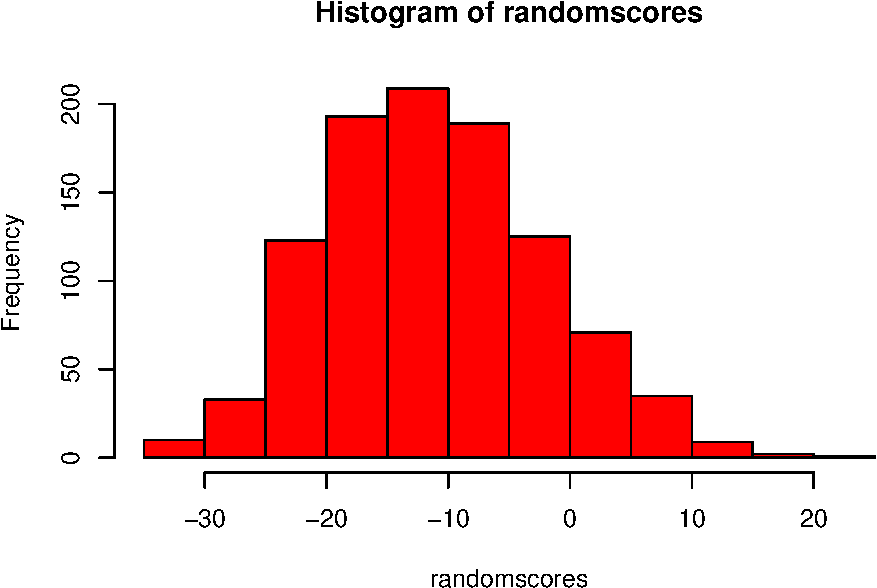
\includegraphics{lbrb_files/figure-latex/unnamed-chunk-286-1.pdf}

We can see from the histogram that quite a lot of the random sequences seem to have higher alignment scores than -5 when aligned to `HEAGAWGHEE' (where -5 is the alignment score for `PAWHEAE' and `HEAGAWGHEE').

We can use the vector randomscores of scores for 1000 alignments of random sequences to `HEAGAWGHEE' to calculate the probability of getting a score as large as the real alignment score for `PAWHEAE' and `HEAGAWGHEE' (ie. -5) by chance.

\begin{Shaded}
\begin{Highlighting}[]
\FunctionTok{sum}\NormalTok{(randomscores }\SpecialCharTok{\textgreater{}=} \SpecialCharTok{{-}}\DecValTok{5}\NormalTok{)}
\end{Highlighting}
\end{Shaded}

\begin{verbatim}
## [1] 276
\end{verbatim}

We see that 266 of the 1000 alignments of random sequences to `HEAGAWGHEE' had alignment scores that were equal to or greater than -5. Thus, we can estimate that the probability of getting a score as large as the real alignment score by chance is (266/1000 =) 0.266. In other words, we can calculate a P-value of 0.266. This probability or P-value is quite high (almost 30\%, or 1 in 3), so we can conclude that it is quite probable that we could get an alignment score as high as -5 by chance alone. This indicates that the sequences `HEAGAWGHEE' and `PAWHEAE' are not more similar than any two random sequences, and so they are probably not related sequences.

Another way of saying this is that the P-value that we calculated is high (0.266), and as a result we conclude that the alignment score for the sequences `HEAGAWGHEE' and `PAWHEAE' is not statistically significant. Generally, if the P-value that we calculate for an alignment of two sequences is \textgreater0.05, we conclude that the alignment score is not statistically significant, and that the sequences are probably not related. On the other hand, if the P-value is less than or equal to 0.05, we conclude that the alignment score is statistically significant, and the sequences are very probably related (homologous).

\hypertarget{summary-4}{%
\section{Summary}\label{summary-4}}

In this practical, you will have learned to use the following R functions:

data() for reading in data that comes with an R package
double() for creating a numeric vector for storing real (non-integer) numbers
toupper() for converting a string of characters from lowercase to uppercase
All of these functions belong to the standard installation of R.

You have also learned the following R functions that belong to the bioinformatics packages:

nucleotideSubstitutionMatrix() in the Biostrings package for making a nucleotide scoring matrix
pairwiseAlignment() in the Biostrings package for making a global alignment between two sequences
c2s() in the SeqinR package for converting a sequence stored in a vector to a string of characters
Links and Further Reading
Some links are included here for further reading.

For background reading on sequence alignment, it is recommended to read Chapter 3 of Introduction to Computational Genomics: a case studies approach by Cristianini and Hahn (Cambridge University Press; www.computational-genomics.net/book/).

For more in-depth information and more examples on using the SeqinR package for sequence analysis, look at the SeqinR documentation, \url{http://pbil.univ-lyon1.fr/software/seqinr/doc.php?lang=eng}.

There is also a very nice chapter on ``Analyzing Sequences'', which includes examples of using SeqinR and Biostrings for sequence analysis, as well as details on how to implement algorithms such as Needleman-Wunsch and Smith-Waterman in R yourself, in the book Applied statistics for bioinformatics using R by Krijnen (available online at cran.r-project.org/doc/contrib/Krijnen-IntroBioInfStatistics.pdf).

For a more in-depth introduction to R, a good online tutorial is available on the ``Kickstarting R'' website, cran.r-project.org/doc/contrib/Lemon-kickstart.

There is another nice (slightly more in-depth) tutorial to R available on the ``Introduction to R'' website, cran.r-project.org/doc/manuals/R-intro.html.

For more information on and examples using the Biostrings package, see the Biostrings documentation at \url{http://www.bioconductor.org/packages/release/bioc/html/Biostrings.html}.

Acknowledgements
Many of the ideas for the examples and exercises for this practical were inspired by the Matlab case study on the Eyeless protein (www.computational-genomics.net/case\_studies/eyeless\_demo.html) from the website that accompanies the book Introduction to Computational Genomics: a case studies approach by Cristianini and Hahn (Cambridge University Press; www.computational-genomics.net/book/).

The examples of DNA sequences and protein sequences to align (`GAATTC' and `GATTA', and sequences `PAWHEAE' and `HEAGAWGHEE'), as well as some ideas related to finding the statistical significance of a pairwise alignment, were inspired by the chapter on ``Analyzing Sequences'' in the book Applied statistics for bioinformatics using R by Krijnen (cran.r-project.org/doc/contrib/Krijnen-IntroBioInfStatistics.pdf).

Thank you to Jean Lobry and Simon Penel for helpful advice on using the SeqinR package.

Contact
I will be grateful if you will send me (Avril Coghlan) corrections or suggestions for improvements to my email address \href{mailto:alc@sanger.ac.uk}{\nolinkurl{alc@sanger.ac.uk}}

License
The content in this book is licensed under a Creative Commons Attribution 3.0 License.

Exercises
Answer the following questions, using the R package. For each question, please record your answer, and what you typed into R to get this answer.

Model answers to the exercises are given in Answers to the exercises on Sequence Alignment.

\begin{enumerate}
\def\labelenumi{\arabic{enumi}.}
\tightlist
\item
  Download FASTA-format files of the Brugia malayi Vab-3 protein (UniProt accession A8PZ80) and the Loa loa Vab-3 protein (UniProt accession E1FTG0) sequences from UniProt.
  Note: the vab-3 gene of Brugia malayi and the vab-3 gene of Loa loa are related genes that control eye development in these two species. Brugia malayi and Loa loa are both parasitic nematode worms, which both cause filariasis, which is classified by the WHO as a neglected tropical disease.
\item
  What is the alignment score for the optimal global alignment between the Brugia malayi Vab-3 protein and the Loa loa Vab-3 protein, when you use the BLOSUM50 scoring matrix, a gap opening penalty of -10 and a gap extension penalty of -0.5?
  Note: to specify a gap opening penalty of -10 and a gap extension penalty of -0.5, set the ``gapOpening'' argument to -9.5, and the ``gapExtension'' penalty to -0.5 in the pairwiseAlignment() function.
\item
  Use the printPairwiseAlignment() function to view the optimal global alignment between \emph{Brugia malayi} Vab-3 protein and the Loa loa Vab-3 protein, using the BLOSUM50 scoring matrix, a gap opening penalty of -10 and a gap extension penalty of -0.5.
  Do you see any regions where the alignment is very good (lots of identities and few gaps)?
\item
  What global alignment score do you get for the two Vab-3 proteins, when you use the BLOSUM62 alignment matrix, a gap opening penalty of -10 and a gap extension penalty of -0.5?
  Which scoring matrix do you think is more appropriate for using for this pair of proteins: BLOSUM50 or BLOSUM62?
\item
  What is the statistical significance of the optimal global alignment for the Brugia malayi and Loa loa Vab-3 proteins made using the BLOSUM50 scoring matrix, with a gap opening penalty of -10 and a gap extension penalty of -0.5?
  In other words, what is the probability of getting a score as large as the real alignment score for Vab-3 by chance?
\item
  What is the optimal global alignment score between the Brugia malayi Vab-6 protein and the Mycobacterium leprae chorismate lyase protein?
  Is the alignment score statistically significant (what is the P- value?)? Does this surprise you?
\end{enumerate}

\hypertarget{computational-gene-finding}{%
\chapter{Computational gene finding}\label{computational-gene-finding}}

\begin{Shaded}
\begin{Highlighting}[]
\FunctionTok{library}\NormalTok{(compbio4all)}
\end{Highlighting}
\end{Shaded}

\textbf{By}: Avril Coghlan.

\textbf{Adapted, edited and expanded}: Nathan Brouwer under the Creative Commons 3.0 Attribution License \href{https://creativecommons.org/licenses/by/3.0/}{(CC BY 3.0)}.

\hypertarget{the-genetic-code}{%
\section{The genetic code}\label{the-genetic-code}}

A protein-coding gene starts with an ``ATG'', which is followed by an integer (whole) number of codons (DNA triplets) that code for amino acids, and ends with a ``TGA'', ``TAA'', or ``TAG''. That is, the start codon of a gene is always ``ATG'', while the stop codon of a gene can be ``TGA'', ``TAA'' or ``TAG''.

In R, you can view the standard genetic code, the correspondence between codons and the amino acids that they are translated into, by using the tablecode() function in the SeqinR package:

\begin{Shaded}
\begin{Highlighting}[]
\FunctionTok{library}\NormalTok{(seqinr)}
\NormalTok{seqinr}\SpecialCharTok{::}\FunctionTok{tablecode}\NormalTok{()}
\end{Highlighting}
\end{Shaded}

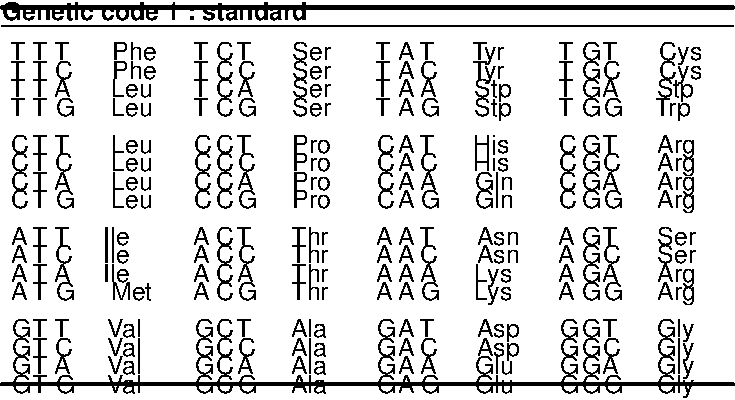
\includegraphics{lbrb_files/figure-latex/unnamed-chunk-289-1.pdf}

You can see from this table that ``ATG'' is translated to Met (the amino acid methionine), and that ``TAA'', ``TGA'' and ``TAG'' correspond to Stp (stop codons, which are not translated to any amino acid, but signal the end of translation).

Finding start and stop codons in a DNA sequence
To look for all the potential start and stop codons in a DNA sequence, we need to find all the ``ATG''s, ``TGA''s, ``TAA''s, and ``TAG''s in the sequence.

To do this, we can use the ``matchPattern()'' function from the Biostrings R package, which identifies all occurrences of a particular motif (eg. ``ATG'') in a sequence. As input, the matchPattern() function requires that the sequences be in the form of a string of single characters.

For example, we can look for all ``ATG''s in the sequence ``AAAATGCAGTAACCCATGCCC'' by typing:

\begin{Shaded}
\begin{Highlighting}[]
\FunctionTok{library}\NormalTok{(}\StringTok{"Biostrings"}\NormalTok{)}
\end{Highlighting}
\end{Shaded}

\begin{Shaded}
\begin{Highlighting}[]
\NormalTok{s1 }\OtherTok{\textless{}{-}} \StringTok{"aaaatgcagtaacccatgccc"}
\end{Highlighting}
\end{Shaded}

\begin{Shaded}
\begin{Highlighting}[]
\FunctionTok{matchPattern}\NormalTok{(}\StringTok{"atg"}\NormalTok{, s1) }\CommentTok{\# Find all ATGs in the sequence s1}
\end{Highlighting}
\end{Shaded}

\begin{verbatim}
## Views on a 21-letter BString subject
## subject: aaaatgcagtaacccatgccc
## views:
##       start end width
##   [1]     4   6     3 [atg]
##   [2]    16  18     3 [atg]
\end{verbatim}

The output from matchPattern() tells us that there are two ``ATG''s in the sequence, at nucleotides 4-6, and at nucleotides 16-18. In fact, we can see these by looking at the sequence ``AAAATGCAGTAACCCATGCCC''.

Similarly, if you use matchPattern() to find the positions of ``TAA''s, ``TGA''s, and ``TAG''s in the sequence ``AAAATGCAGTAACCCATGCCC'', you will find that it has one ``TAA'' at nucleotides 10-12, but no ``TAG''s or ``TGA''s.

The following R function ``findPotentialStartsAndStops()'' can be used to find all potential start and stop codons in a DNA sequence:

To use the function, you will need to copy and paste it into R. For example, we can use this function to find potential start and stop codons in sequence s1:

\begin{Shaded}
\begin{Highlighting}[]
\NormalTok{s1 }\OtherTok{\textless{}{-}} \StringTok{"aaaatgcagtaacccatgccc"}
\FunctionTok{findPotentialStartsAndStops}\NormalTok{(s1)}
\end{Highlighting}
\end{Shaded}

\begin{verbatim}
## [[1]]
## [1]  4 10 16
## 
## [[2]]
## [1] "atg" "taa" "atg"
\end{verbatim}

The result of the function is returned as a list variable that contains two elements: the first element of the list is a vector containing the positions of potential start and stop codons in the input sequence, and the second element of the list is a vector containing the type of those start/stop codons (``atg'', ``taa'', ``tag'', or ``tga'').

The output for sequence s1 tells us that sequence s1 has an ``ATG'' starting at nucleotide 4, a ``TAA'' starting at nucleotide 10, and another ``ATG'' starting at nucleotide 16.

We can use the function findPotentialStartsAndStops() to find all potential start and stop codons in longer sequences. For example, say we want to find all potential start and stop codons in the first 500 nucleotides of the genome sequence of the DEN-1 Dengue virus (NCBI accession NC\_001477).

In a previous chapter, you learned that you can retrieve a sequence for an NCBI accession using the ``getncbiseq()'' function. Thus, to retrieve the genome sequence of the DEN-1 Dengue virus (NCBI accession NC\_001477), we can type:

\begin{Shaded}
\begin{Highlighting}[]
\NormalTok{dengueseq }\OtherTok{\textless{}{-}}\NormalTok{ rentrez}\SpecialCharTok{::}\FunctionTok{entrez\_fetch}\NormalTok{(}\AttributeTok{db =} \StringTok{"nucleotide"}\NormalTok{, }
                          \AttributeTok{id =} \StringTok{"NC\_001477"}\NormalTok{, }
                          \AttributeTok{rettype =} \StringTok{"fasta"}\NormalTok{)}

\NormalTok{dengueseq }\OtherTok{\textless{}{-}} \FunctionTok{gsub}\NormalTok{(}\StringTok{"}\SpecialCharTok{\textbackslash{}n}\StringTok{"}\NormalTok{, }\StringTok{""}\NormalTok{, dengueseq)}
\NormalTok{header. }\OtherTok{\textless{}{-}} \StringTok{"\textgreater{}NC\_001477.1 Dengue virus 1, complete genome"}
\NormalTok{dengueseq }\OtherTok{\textless{}{-}} \FunctionTok{gsub}\NormalTok{(header.,}\StringTok{""}\NormalTok{, dengueseq)}
\end{Highlighting}
\end{Shaded}

The variable dengueseq is a vector variable, and each letter in the DEN-1 Dengue virus DNA sequence is stored in one element of this vector.

Dengue virus causes Dengue fever, which is classified as a neglected tropical disease by the WHO.

To cut out the first 500 nucleotides of the DEN-1 Dengue virus sequence, we can just take the first 500 elements of this vector:

\begin{Shaded}
\begin{Highlighting}[]
\NormalTok{dengueseqstart }\OtherTok{\textless{}{-}}\NormalTok{ dengueseq[}\DecValTok{1}\SpecialCharTok{:}\DecValTok{500}\NormalTok{] }
\end{Highlighting}
\end{Shaded}

Find the length of the ``dengueseqstart'' start vector

\begin{Shaded}
\begin{Highlighting}[]
\FunctionTok{length}\NormalTok{(dengueseqstart)             }
\end{Highlighting}
\end{Shaded}

Next we want to find potential start and stop codons in the first 500 nucleotides of the Dengue virus sequence. We can do this using the findPotentialStartsAndStops() function described above. However, the findPotentialStartsAndStops() function requires that the input sequence be in the format of a string of characters, rather than a vector. Therefore, we first need to convert the vector dengueseqstart into a string of characters. We can do that using the c2s() function in the SeqinR package:

\begin{Shaded}
\begin{Highlighting}[]
\FunctionTok{library}\NormalTok{(}\StringTok{"seqinr"}\NormalTok{)                 }\CommentTok{\# Load the SeqinR package}
\end{Highlighting}
\end{Shaded}

\begin{Shaded}
\begin{Highlighting}[]
\NormalTok{dengueseqstart                    }\CommentTok{\# Print out the vector dengueseqstart}
\end{Highlighting}
\end{Shaded}

\begin{Shaded}
\begin{Highlighting}[]
\NormalTok{dengueseqstartstring }\OtherTok{\textless{}{-}} \FunctionTok{c2s}\NormalTok{(dengueseqstart) }\CommentTok{\# Convert the vector "dengueseqstart" to a string of characters}
\end{Highlighting}
\end{Shaded}

Print out the variable string of characters ``dengueseqstartstring''

\begin{Shaded}
\begin{Highlighting}[]
\NormalTok{dengueseqstartstring                      }
\end{Highlighting}
\end{Shaded}

We can then find potential start and stop codons in the first 500 nucleotides of the DEN-1 Dengue virus sequence by typing:

\begin{Shaded}
\begin{Highlighting}[]
\FunctionTok{findPotentialStartsAndStops}\NormalTok{(dengueseqstartstring)}
\end{Highlighting}
\end{Shaded}

We see that the lambda sequence has many different potential start and stop codons, for example, a potential stop codon (TAG) at nucleotide 7, a potential stop codon (TAA) at nucleotide 53, a potential stop codon (TAG) at nucleotide 58, and so on.

\hypertarget{reading-frames}{%
\section{Reading frames}\label{reading-frames}}

Potential start and stop codons in a DNA sequence can be in three different possible reading frames. A potential start/stop codon is said to be in the +1 reading frame if there is an integer number of triplets x between the first nucleotide of the sequence and the start of the start/stop codon. Thus, a potential start/stop codon that begins at nucleotides 1 (0 triplets), 4 (1 triplet), 7 (2 triplets)\ldots{} will be in the +1 reading frame.

If there is an integer number of triplets x, plus one nucleotide (ie. x.3 triplets), between the first nucleotide of the sequence and the start of the start/stop codon, then the start/stop codon is said to be in the +2 reading frame. A potential start/stop codon that begins at nucleotides 2 (0.3 triplets), 5 (1.3 triplets), 8 (2.3 triplets) \ldots{} is in the +2 reading frame.

Similarly, if there is an integer number of triplets x, plus two nucleotides (ie. x.6 triplets), between the first nucleotides of the sequence and the start of the start/stop codon, the start/stop codon is in the +3 reading frame. So a potential start/stop codon that begins at nucleotides 3 (0.6 triplets), 6 (1.6 triplets), 9 (2.6 triplets)\ldots{} is in the +3 reading frame.

For a potential start and stop codon to be part of the same gene, they must be in the same reading frame.

From the output of findPotentialStartsAndStops() for the first 500 nucleotides of the genome of DEN-1 Dengue virus (see above), you can see that there is a potential start codon (ATG) that starts at nucleotide 137, and a potential stop codon (TGA) that starts at nucleotide 141. That is, the potential start codon is from nucleotides 137-139 and the potential stop codon is from nucleotides 141-143. Could the region from nucleotides 137 to 143 possibly be a gene?

We can cut out the region from nucleotides 137 to 143 of the sequence dengueseqstartstring to have a look, by using the substring() function. If you look at the help page for the substring() function, you will see that its arguments (inputs) are the name of the variable containing the string of characters (ie., the DNA sequence), and the coordinates of the substring that you want:

\begin{Shaded}
\begin{Highlighting}[]
\FunctionTok{substring}\NormalTok{(dengueseqstartstring,}\DecValTok{137}\NormalTok{,}\DecValTok{143}\NormalTok{)}
\end{Highlighting}
\end{Shaded}

If we look at the sequence from nucleotides 137-143, ``ATGCTGA'', we see that it starts with a potential start codon (ATG) and ends with a potential stop codon (TGA).

However, the ribosome reads the sequence by scanning the codons (triplets) one-by-one from left to right, and when we break up the sequence into codons (triplets) we see that it does not contain an integer (whole) number of triplets: ``ATG CTG A''.

This means that even if the ribosome will not recognise the region from 137-143 as a potential gene, as the ATG at nucleotide 137 is not separated from the TGA at nucleotide 141 by an integer number of codons. That is, this ATG and TGA are not in the same reading frame, and so cannot be the start and stop codon of the same gene.

The potential start codon at nucleotide 137 of the lambdaseqstartstring sequence is in the +2 reading frame, as there is an integer number of triplets, plus one nucleotide, between the start of the sequence and the start of the start codon (ie. triplets 1-3, 4-6, 7-9, 10-12, 13-15, 16-18, 19-21, 22-24, 25-27, 28-30, \ldots, 133-135, and a single nucleotide 136).

However, the potential stop codon at nucleotide 141 is the +3 reading frame, as there are two nucleotides plus an integer number of triplets between the start of the sequence and the start of the stop codon (ie. triplets 1-3, 4-6, 7-9, 10-12, 13-15, 16-18, 19-21, 22-24, 25-27, 28-30, 31-33, 34-36, 37-39, 40-42, 43-45, \ldots, 133-135, 136-138, and two nucleotides 139, 140).

As the potential start codon at nucleotide 137 and the potential stop codon at nucleotide 141 are in different reading frames, they are not separated by an integer number of codons, and therefore cannot be part of the same gene.

\hypertarget{finding-open-reading-frames-on-the-forward-strand-of-a-dna-sequence}{%
\section{Finding open reading frames on the forward strand of a DNA sequence}\label{finding-open-reading-frames-on-the-forward-strand-of-a-dna-sequence}}

To find potential genes, we need to look for a potential start codon, followed by an integer number of codons, followed by a potential stop codon. This is eqivalent to looking for a potential start codon followed by a potential stop codon that is in the same reading frame. Such a stretch of DNA is known as an open reading frame (ORF), and is a good candidate for a potential gene.

The following function plotPotentialStartsAndStops() plots the potential start and stop codons in the three different reading frames of a DNA sequence:

To use this function, you will first need to copy and paste it into R.

For example, to plot the potential start and stop codons in the first 500 nucleotides of the DEN-1 Dengue virus genome, we type:

\begin{Shaded}
\begin{Highlighting}[]
\FunctionTok{plotPotentialStartsAndStops}\NormalTok{(dengueseqstartstring)}
\end{Highlighting}
\end{Shaded}

In the picture produced by plotPotentialStartsAndStops(), the x-axis represents the input sequence (dengueseqstartstring here). The potential start codons are represented by vertical red lines, and potential stop codons are represented by vertical blue lines.

Three different layers in the picture show potential start/stop codons in the +1 reading frame (bottom layer), +2 reading frame (middle layer), and +3 reading frame (top layer).

We can see that the start codon at nucleotide 137 is represented by a vertical red line in the layer corresponding to the +2 reading frame (middle layer). There are no potential stop codons in the +2 reading frame to the right of that start codon. Thus, the start codon at nucleotide 137 does not seem to be part of an open reading frame.

We can see however that in the +3 reading frame (top layer) there is a predicted start codon (red line) at position 318 and that this is followed by a predicted stop codon (blue line) at position 371. Thus, the region from nucleotides 318 to 371 could be a potential gene in the +3 reading frame. In other words, the region from nucleotides 318 to 371 is an open reading frame, or ORF.

For example, we can use findORFsinSeq to find all ORFs in the sequence s1:

\begin{Shaded}
\begin{Highlighting}[]
\NormalTok{s1 }\OtherTok{\textless{}{-}} \StringTok{"aaaatgcagtaacccatgccc"}
\end{Highlighting}
\end{Shaded}

\begin{Shaded}
\begin{Highlighting}[]
\FunctionTok{findORFsinSeq}\NormalTok{(s1)}
\end{Highlighting}
\end{Shaded}

The function findORFsinSeq() returns a list variable, where the first element of the list is a vector of the start positions of ORFs, the second element of the list is a vector of the end positions of those ORFs, and the third element is a vector containing the lengths of the ORFs.

The output for the findORFsinSeq() function for s1 tells us that there is one ORF in the sequence s1, and that the predicted start codon starts at nucleotide 4 in the sequence, and that the predicted stop codon ends at nucleotide 12 in the sequence.

We can use the function findORFsinSeq() to find the ORFs in the first 500 nucleotides of the DEN-1 Dengue virus genome sequence by typing:

\begin{Shaded}
\begin{Highlighting}[]
\FunctionTok{findORFsinSeq}\NormalTok{(dengueseqstartstring)}
\end{Highlighting}
\end{Shaded}

The result from findORFsinSeq() indicates that there are two ORFs in the first 500 nucleotides of the DEN-1 Dengue virus genome, at nucleotides 298-480 (start codon at 298-300, stop codon at 478-480), and 318-371 (start codon at 318-320, stop codon at 369-371).

The following function ``plotORFsinSeq()'' plots the positions of ORFs in a sequence:

To use this function, you will first need to copy and paste it into R. You can then use this function to plot the positions of the ORFs in dengueseqstartstring by typing:

\begin{Shaded}
\begin{Highlighting}[]
\FunctionTok{plotORFsinSeq}\NormalTok{(dengueseqstartstring)}
\end{Highlighting}
\end{Shaded}

The picture produced by plotORFsinSeq() represents the two ORFs in the first 500 nucleotides of the lambda genome as blue rectangles.

One of the ORFs is in the +3 reading frame, and one is in the +1 reading frame. There are no ORFs in the +2 reading frame, as there are no potential stop codons to the right (3') of the potential start codons in the +2 reading frame, as we can see from the picture produced by plotPotentialStartsAndStops() above.

Predicting the protein sequence for an ORF
If you find an ORF in a DNA sequence, it is interesting to find the DNA sequence of the ORF. For example, the function findORFsinSeq() indicates that there is an ORF from nucleotides 4-12 of the sequence s1 (aaaatgcagtaacccatgccc). To look at the DNA sequence for just the ORF, we can use the substring() function to cut out that piece of DNA. For example, to cut out the substring of sequence s1 that corresponds to the ORF from nucleotides 4-12, we type:

\begin{Shaded}
\begin{Highlighting}[]
\NormalTok{s1 }\OtherTok{\textless{}{-}} \StringTok{"aaaatgcagtaacccatgccc"}
\end{Highlighting}
\end{Shaded}

\begin{Shaded}
\begin{Highlighting}[]
\NormalTok{myorf }\OtherTok{\textless{}{-}} \FunctionTok{substring}\NormalTok{(s1, }\DecValTok{4}\NormalTok{, }\DecValTok{12}\NormalTok{)}
\end{Highlighting}
\end{Shaded}

\begin{Shaded}
\begin{Highlighting}[]
\NormalTok{myorf }\CommentTok{\# Print out the sequence of "myorf"}
\end{Highlighting}
\end{Shaded}

As you can see, the ORF starts with a predicted start codon (ATG), is followed by an integer number of codons (just one codon, CAG, in this case), and ends with a predicted stop codon (TAA).

If you have the DNA sequence of an ORF, you can predict the protein sequence for the ORF by using the translate() function from the SeqinR package. Note that as there is a function called translate() in both the Biostrings and SeqinR packages, we need to type seqinr::translate() to specify that we want to use the SeqinR translate() function.

The translate() function requires that the input sequence be in the form of a vector of characters. If your sequence is in the form of a string of characters, you can convert it to a vector of characters using the s2c() function from the SeqinR package. For example, to predict the protein sequence of the ORF myorf, you would type:

\begin{Shaded}
\begin{Highlighting}[]
\NormalTok{myorfvector }\OtherTok{\textless{}{-}} \FunctionTok{s2c}\NormalTok{(myorf) }\CommentTok{\# Convert the sequence of characters to a vector}
\end{Highlighting}
\end{Shaded}

\begin{Shaded}
\begin{Highlighting}[]
\NormalTok{myorfvector               }\CommentTok{\# Print out the value of "myorfvector"}
\end{Highlighting}
\end{Shaded}

\begin{Shaded}
\begin{Highlighting}[]
\NormalTok{seqinr}\SpecialCharTok{::}\FunctionTok{translate}\NormalTok{(myorfvector)}
\end{Highlighting}
\end{Shaded}

From the output of the seqinr::translate() function, we see that the predicted start codon (ATG) is translated as a Methionine (M), and that this is followed by a Glutamine (Q). The predicted stop codon is represented as ``*'' as it is not translated into any amino acid.

Finding open reading frames on the reverse strand of a DNA sequence
Genes in a genome sequence can occur either on the forward (plus) strand of the DNA, or on the reverse (minus) strand. To find ORFs on the reverse strand of a sequence, we must first infer the reverse strand sequence, and then use our findORFsinSeq() function to find ORFs on the reverse strand.

The reverse strand sequence easily can be inferred from the forward strand sequence, as it is always the reverse complement sequence of the forward strand sequence. We can use the comp() function from the SeqinR package to calculate the complement of a sequence, and the rev() function to reverse that sequence in order to give us the reverse complement sequence.

The comp() and rev() functions require that the input sequence is in the form of a vector of characters. The s2c() function can be used to convert a sequence in the form of a string of characters to a vector, while the c2s() function is useful for convering a vector back to a string of characters.

For example, if our forward strand sequence is ``AAAATGCTTAAACCATTGCCC'', and we want to find the reverse strand sequence, we type:

\begin{Shaded}
\begin{Highlighting}[]
\NormalTok{forward }\OtherTok{\textless{}{-}} \StringTok{"AAAATGCTTAAACCATTGCCC"}
\end{Highlighting}
\end{Shaded}

\begin{Shaded}
\begin{Highlighting}[]
\NormalTok{forwardvector }\OtherTok{\textless{}{-}} \FunctionTok{s2c}\NormalTok{(forward)                }\CommentTok{\# Convert the string of characters to a vector}
\end{Highlighting}
\end{Shaded}

\begin{Shaded}
\begin{Highlighting}[]
\NormalTok{forwardvector                                }\CommentTok{\# Print out the vector containing the forward strand sequence}
\end{Highlighting}
\end{Shaded}

\begin{verbatim}
##  [1] "A" "A" "A" "A" "T" "G" "C" "T" "T" "A" "A" "A" "C" "C" "A" "T" "T" "G" "C"
## [20] "C" "C"
\end{verbatim}

\begin{Shaded}
\begin{Highlighting}[]
\NormalTok{reversevector }\OtherTok{\textless{}{-}} \FunctionTok{rev}\NormalTok{(}\FunctionTok{comp}\NormalTok{(forwardvector))    }\CommentTok{\# Find the reverse strand sequence, by finding the reverse complement}
\end{Highlighting}
\end{Shaded}

Print out the vector containing the reverse strand sequence

\begin{Shaded}
\begin{Highlighting}[]
\NormalTok{reversevector                             }
\end{Highlighting}
\end{Shaded}

\begin{verbatim}
##  [1] "g" "g" "g" "c" "a" "a" "t" "g" "g" "t" "t" "t" "a" "a" "g" "c" "a" "t" "t"
## [20] "t" "t"
\end{verbatim}

Convert the vector to a string of characters

\begin{Shaded}
\begin{Highlighting}[]
\NormalTok{reverse }\OtherTok{\textless{}{-}} \FunctionTok{c2s}\NormalTok{(reversevector)                }
\end{Highlighting}
\end{Shaded}

Print out the string of characters containing the reverse strand sequence

\begin{Shaded}
\begin{Highlighting}[]
\NormalTok{reverse                                      }
\end{Highlighting}
\end{Shaded}

\begin{verbatim}
## [1] "gggcaatggtttaagcatttt"
\end{verbatim}

In the command reversevector \textless- rev(comp(forwardvector)) above, we are first using the comp() function to find the complement of the forward strand sequence. We are then using the rev() function to take the output sequence given by comp() and reverse the order of the letters in that sequence. An equivalent way of doing the same thing would be to type:

Find the complement of the forward strand sequence

\begin{Shaded}
\begin{Highlighting}[]
\NormalTok{complement }\OtherTok{\textless{}{-}} \FunctionTok{comp}\NormalTok{(forwardvector)            }
\end{Highlighting}
\end{Shaded}

Reverse the order of the letters in sequence ``complement'', to
find the reverse strand sequence (the reverse complement sequence)

\begin{Shaded}
\begin{Highlighting}[]
\NormalTok{reversevector }\OtherTok{\textless{}{-}} \FunctionTok{rev}\NormalTok{(complement)             }\CommentTok{\# }
\end{Highlighting}
\end{Shaded}

Once we have inferred the reverse strand sequence, we can then use the findORFsinSeq() function to find ORFs in the reverse strand sequence:

\begin{Shaded}
\begin{Highlighting}[]
\FunctionTok{findORFsinSeq}\NormalTok{(reverse)}
\end{Highlighting}
\end{Shaded}

This indicates that there is one ORF of length 9 bp in the reverse strand of sequence ``AAAATGCTTAAACCATTGCCC'', that has a predicted start codon that starts at nucleotide 6 in the reverse strand sequence and a predicted stop codon that ends at nucleotide 14 in the reverse strand sequence.

\hypertarget{lengths-of-open-reading-frames}{%
\section{Lengths of open reading frames}\label{lengths-of-open-reading-frames}}

As you can see from the picture displaying the genetic code made using tablecode() (above), three of the 64 different codons are stop codons. This means that in a random DNA sequence the probability that any codon is a potential stop codon is 3/64, or about 1/21 (about 5\%).

Therefore, you might expect that sometimes potential start and stop codons can occur in a DNA sequence just due to chance alone, not because they are actually part of any real gene that is transcribed and translated into a protein.

As a result, many of the ORFs in a DNA sequence may not correspond to real genes, but just be stretches of DNA between potential start and stop codons that happened by chance to be found in the sequence.

In other words, an open reading frame (ORF) is just a gene prediction, or a potential gene. It may correspond to a real gene (may be a true positive gene prediction), but it may not (may be a false positive gene prediction).

How can we tell whether the potential start and stop codons of an ORF are probably real start and stop codons, that is, whether an ORF probably corresponds to a real gene that is transcribed and translated into a protein?

In fact, we cannot tell using bioinformatics methods alone (we actually need to do some lab experiments to know), but we can make a fairly confident prediction. We can make our prediction based on the length of the ORF.

y definition, an ORF is a stretch of DNA that starts with a potential start codon, and ends with a potential stop codon in the same reading frame, and so has no internal stop codons in that reading frame. Because about 1/21 of codons (\textasciitilde5\%) in a random DNA sequence are expected to be potential stop codons just by chance alone, if we see a very long ORF of hundreds of codons, it would be surprising that there would be no internal stop codons in such a long stretch of DNA if the ORF were not a real gene.

In other words, long ORFs that are hundreds of codons long are unlikely to occur due to chance alone, and therefore we can be fairly confident that such long ORFs probably correspond to real genes.

\hypertarget{significance-of-orfs}{%
\chapter{Significance of ORFs}\label{significance-of-orfs}}

\textbf{By}: Avril Coghlan.

\textbf{Adapted, edited and expanded}: Nathan Brouwer under the Creative Commons 3.0 Attribution License \href{https://creativecommons.org/licenses/by/3.0/}{(CC BY 3.0)}.

\hypertarget{identifying-significant-open-reading-frames}{%
\section{Identifying significant open reading frames}\label{identifying-significant-open-reading-frames}}

How long does an ORF need to be in order for us to be confident that it probably corresponds to a real gene? This is a difficult question.

One approach to answer this is to ask: what is the longest ORF found in a random sequence of the same length and nucleotide composition as our original sequence?

The ORFs in a random sequence do not correspond to real genes, but are just due to potential start and stop codons that have occurred by chance in those sequences (since, by definition, a random sequence is one that was generated randomly, rather than by evolution as in a real organism).

Thus, by looking at the lengths of ORFs in the random sequence, we can see what is the longest ORF that is likely to occur by chance alone.

But where can we get random sequences from? In a previous chapter, you learnt that you can generate random sequences using a multinomial model with a particular probability of each letter (a particular probability of A, C, G, and T in the case of random DNA sequences).

In that previous chapter, we used the function generateSeqsWithMultinomialModel() to generate random sequences using a multinomial model in which the probability of each letter is set equal to the fraction of an input sequence that consists of that letter. This function takes two arguments, the input sequence, and the number of the random sequences that you want to generate.

For example, to create a random sequence of the same length as `AAAATGCTTAAACCATTGCCC', using a multinomial model in which the probabilities of A, C, G and T are set equal to their fractions in this sequence, we copy and paste the generateSeqsWithMultinomialModel() into R, then type:

\begin{Shaded}
\begin{Highlighting}[]
\NormalTok{myseq    }\OtherTok{\textless{}{-}} \StringTok{"AAAATGCTTAAACCATTGCCC"}
\end{Highlighting}
\end{Shaded}

Generate one random sequence using the multinomial model

\begin{Shaded}
\begin{Highlighting}[]
\FunctionTok{generateSeqsWithMultinomialModel}\NormalTok{(myseq, }\DecValTok{1}\NormalTok{) }
\end{Highlighting}
\end{Shaded}

\begin{verbatim}
## [1] "ATAAACCAAATAATAAAGAAA"
\end{verbatim}

We can then use the findORFsinSeq() function to find ORFs in this random sequence. If we repeat this 10 times, we can find the lengths of the ORFs found in the 10 random sequences. We can then compare the lengths of the ORFs found in the original sequence, to the lengths of the ORFs found in the random sequences.

For example, to compare the lengths of ORFs found in the DEN-1 Dengue virus genome sequence dengueseq to the lengths of ORFs found in 10 random sequences generated using a multinomial model in which the probabilities of the four bases are set equal to their fractions in the DEN-1 Dengue virus sequence, we type:

\#Convert the Dengue sequence to a string of characters

\begin{Shaded}
\begin{Highlighting}[]
\NormalTok{dengueseqstring }\OtherTok{\textless{}{-}} \FunctionTok{c2s}\NormalTok{(dengueseq)   }
\end{Highlighting}
\end{Shaded}

Find ORFs in ``dengueseqstring''

\begin{Shaded}
\begin{Highlighting}[]
\NormalTok{mylist }\OtherTok{\textless{}{-}} \FunctionTok{findORFsinSeq}\NormalTok{(dengueseqstring)  }
\end{Highlighting}
\end{Shaded}

Find the lengths of ORFs in ``dengueseqstring''

\begin{Shaded}
\begin{Highlighting}[]
\NormalTok{orflengths }\OtherTok{\textless{}{-}}\NormalTok{ mylist[[}\DecValTok{3}\NormalTok{]]  }
\end{Highlighting}
\end{Shaded}

Generate 10 random sequences using the multinomial model

\begin{Shaded}
\begin{Highlighting}[]
\NormalTok{randseqs }\OtherTok{\textless{}{-}} \FunctionTok{generateSeqsWithMultinomialModel}\NormalTok{(dengueseqstring, }\DecValTok{10}\NormalTok{) }
\end{Highlighting}
\end{Shaded}

Tell R that we want to make a new vector of numbers

\begin{Shaded}
\begin{Highlighting}[]
\NormalTok{randseqorflengths }\OtherTok{\textless{}{-}} \FunctionTok{numeric}\NormalTok{()            }
\end{Highlighting}
\end{Shaded}

\begin{Shaded}
\begin{Highlighting}[]
\ControlFlowTok{for}\NormalTok{ (i }\ControlFlowTok{in} \DecValTok{1}\SpecialCharTok{:}\DecValTok{10}\NormalTok{)}
\NormalTok{  \{}
     \FunctionTok{print}\NormalTok{(i)}
\NormalTok{     randseq }\OtherTok{\textless{}{-}}\NormalTok{ randseqs[i]                     }\CommentTok{\# Get the ith random sequence}
\NormalTok{     mylist }\OtherTok{\textless{}{-}} \FunctionTok{findORFsinSeq}\NormalTok{(randseq)           }\CommentTok{\# Find ORFs in "randseq"}
\NormalTok{     lengths }\OtherTok{\textless{}{-}}\NormalTok{ mylist[[}\DecValTok{3}\NormalTok{]]                     }\CommentTok{\# Find the lengths of ORFs in "randseq"}
\NormalTok{     randseqorflengths }\OtherTok{\textless{}{-}} \FunctionTok{append}\NormalTok{(randseqorflengths, lengths, }\AttributeTok{after=}\FunctionTok{length}\NormalTok{(randseqorflengths))}
\NormalTok{  \}}
\end{Highlighting}
\end{Shaded}

This may take a little time to run, however, the for loop above prints out the value of i each time that it starts the loop, so you can see how far it has got.

In the code above, we retrieve the lengths of the ORFs found by function findORFsinSeq() by taking the third element of the list returned by this function. As mentioned above, the third element of the list returned by this function is a vector containing the lengths of all the ORFs found in the input sequence.

We can then plot a histogram of the lengths of the ORFs in the real DEN-1 Dengue genome sequence (orflengths) beside a histogram of the lengths of the ORFs in the 10 random sequences (randseqorflengths):

\begin{Shaded}
\begin{Highlighting}[]
\FunctionTok{par}\NormalTok{(}\AttributeTok{mfrow =} \FunctionTok{c}\NormalTok{(}\DecValTok{1}\NormalTok{,}\DecValTok{2}\NormalTok{))                      }\CommentTok{\# Make a picture with two plots side{-}by{-}side (one row, two columns)}
\NormalTok{bins }\OtherTok{\textless{}{-}} \FunctionTok{seq}\NormalTok{(}\DecValTok{0}\NormalTok{,}\DecValTok{11000}\NormalTok{,}\DecValTok{50}\NormalTok{)                  }\CommentTok{\# Set the bins for the histogram}
\FunctionTok{hist}\NormalTok{(randseqorflengths, }\AttributeTok{breaks=}\NormalTok{bins, }\AttributeTok{col=}\StringTok{"red"}\NormalTok{, }\AttributeTok{xlim=}\FunctionTok{c}\NormalTok{(}\DecValTok{0}\NormalTok{,}\DecValTok{1000}\NormalTok{))}
\FunctionTok{hist}\NormalTok{(orflengths, }\AttributeTok{breaks=}\NormalTok{bins, }\AttributeTok{col=}\StringTok{"red"}\NormalTok{, }\AttributeTok{xlim=}\FunctionTok{c}\NormalTok{(}\DecValTok{0}\NormalTok{,}\DecValTok{1000}\NormalTok{))}
\end{Highlighting}
\end{Shaded}

In other words, the histogram of the lengths of the ORFs in the 10 random sequences gives us an idea of the length distribution of ORFs that you would expect by chance alone in a random DNA sequence (generated by a multinomial model in which the probabilities of the four bases are set equal to their frequencies in the DEN-1 Dengue virus genome sequence).

We can calculate the longest of the ORFs that occurs in the random sequences, using the max() function, which can be used to find the largest element in a vector of numbers:

\begin{Shaded}
\begin{Highlighting}[]
\FunctionTok{max}\NormalTok{(randseqorflengths)}
\end{Highlighting}
\end{Shaded}

This indicates that the longest ORF that occurs in the random sequences is 342 nucleotides long. Thus, it is possible for an ORF of up to 342 nucleotides to occur by chance alone in a random sequence of the same length and roughly the same composition as the DEN-1 Dengue virus genome.

Therefore, we could use 342 nucleotides as a threshold, and discard all ORFs found in the DEN-1 Dengue virus genome that are shorter than this, under the assumption that they probably arose by chance and probably do not correspond to real genes. How many ORFs would be left in the DEN-1 Dengue virus genome sequence if we used 342 nucleotides as a threshold?

\begin{Shaded}
\begin{Highlighting}[]
\FunctionTok{summary}\NormalTok{(orflengths)}
\end{Highlighting}
\end{Shaded}

If we did use 342 nucleotides as a threshold, there would only be 1 ORF left in the DEN-1 Dengue virus genome. Some of the 115 shorter ORFs that we discarded may correspond to real genes.

Generally, we don't want to miss many real genes, we may want to use a more tolerant threshold. For example, instead of discarding all Dengue ORFs that are shorter than the longest ORF found in the 10 random sequences, we could discard all Dengue ORFs that are shorter than the longest 99\% of ORFs in the random sequences.

We can use the quantile() function to find quantiles of a set of numbers. The 99th quantile for a set of numbers is the value x such that 99\% of the numbers in the set have values less than x.

For example, to find the 99th quantile of randomseqorflengths, we type:

\begin{Shaded}
\begin{Highlighting}[]
\FunctionTok{quantile}\NormalTok{(randseqorflengths, }\AttributeTok{probs=}\FunctionTok{c}\NormalTok{(}\FloatTok{0.99}\NormalTok{))}
\end{Highlighting}
\end{Shaded}

This means that 99\% of the ORFs in the random sequences have lengths less than 248 nucleotides long. In other words, the longest of the longest 99\% of ORFs in the random sequences is 248 nucleotides.

Thus, if we were using this as a threshold, we would discard all ORFs from the DEN-1 Dengue genome that are 248 nucleotides or shorter. This will result in fewer ORFs being discarded than if we used the more stringent threshold of 342 nucleotides (ie. discarding all ORFs of \textless342 nucleotides), so we will probably have discarded fewer ORFs that correspond to real genes. Unfortunately, it probably means that we will also have kept more false positives at the same time, that is, ORFs that do not correspond to real genes.

\hypertarget{summary-5}{%
\section{Summary}\label{summary-5}}

In this practical, you will have learnt to use the following R functions:

substring() for cutting out a substring of a string of characters (eg. a subsequence of a DNA sequence)
rev() for reversing the order of the elements in a vector
hist() to make a histogram plot
max() to find the largest element in a vector of numbers
quantile() to find quantiles of a set of numbers that correspond to particular probabilities
All of these functions belong to the standard installation of R.

You have also learnt the following R functions that belong to the bioinformatics packages:

tablecode() in the SeqinR package for viewing the genetic code
MatchPattern() in the Biostrings package for finding all occurrences of a motif in a sequence
translate() in the SeqinR package to get the predicted protein sequence for an ORF
s2c() in the SeqinR package to convert a sequence stored as a string of characters into a vector
c2s() in the SeqinR package to convert a sequence stored in a vector into a string of characters
comp() in the SeqinR package to find the complement of a DNA sequence
Links and Further Reading
Some links are included here for further reading.

For background reading on computational gene-finding, it is recommended to read Chapter 2 of Introduction to Computational Genomics: a case studies approach by Cristianini and Hahn (Cambridge University Press; www.computational-genomics.net/book/).

For more in-depth information and more examples on using the SeqinR package for sequence analysis, look at the SeqinR documentation, \url{http://pbil.univ-lyon1.fr/software/seqinr/doc.php?lang=eng}.

For more information on and examples using the Biostrings package, see the Biostrings documentation at \url{http://www.bioconductor.org/packages/release/bioc/html/Biostrings.html}.

There is also a very nice chapter on ``Analyzing Sequences'', which includes examples of using the SeqinR and Biostrings packages for sequence analysis, in the book Applied statistics for bioinformatics using R by Krijnen (available online at cran.r-project.org/doc/contrib/Krijnen-IntroBioInfStatistics.pdf).

For a more in-depth introduction to R, a good online tutorial is available on the ``Kickstarting R'' website, cran.r-project.org/doc/contrib/Lemon-kickstart.

There is another nice (slightly more in-depth) tutorial to R available on the ``Introduction to R'' website, cran.r-project.org/doc/manuals/R-intro.html.

Acknowledgements
Many of the ideas for the examples and exercises for this practical were inspired by the Matlab case study on the Haemophilus influenzae genome (www.computational-genomics.net/case\_studies/haemophilus\_demo.html) from the website that accompanies the book Introduction to Computational Genomics: a case studies approach by Cristianini and Hahn (Cambridge University Press; www.computational-genomics.net/book/).

Thank you to Jean Lobry and Simon Penel for helpful advice on using the SeqinR package.

Exercises
Answer the following questions, using the R package. For each question, please record your answer, and what you typed into R to get this answer.

Model answers to the exercises are given in Answers to the exercises on Computational Gene-finding.

\begin{enumerate}
\def\labelenumi{\arabic{enumi}.}
\tightlist
\item
  How many ORFs are there on the forward strand of the DEN-1 Dengue virus genome (NCBI accession NC\_001477)?
\item
  What are the coordinates of the rightmost (most 3', or last) ORF in the forward strand of the DEN-1 Dengue virus genome?
\item
  What is the predicted protein sequence for the rightmost (most 3', or last) ORF in the forward strand of the DEN-1 Dengue virus genome?
\item
  How many ORFs are there of 30 nucleotides or longer in the forward strand of the DEN-1 Dengue virus genome sequence?
\item
  How many ORFs longer than 248 nucleotides are there in the forward strand of the DEN-1 Dengue genome sequence?
\item
  If an ORF is 248 nucleotides long, what length in amino acids will its predicted protein sequence be?
\item
  How many ORFs are there on the forward strand of the rabies virus genome (NCBI accession NC\_001542)? Note: rabies virus is the virus responsible for rabies, which is classified by the WHO as a neglected tropical disease.
\item
  What is the length of the longest ORF among the 99\% of longest ORFs in 10 random sequences of the same lengths and composition as the rabies virus genome sequence?
\item
  How many ORFs are there in the rabies virus genome that are longer than the threshold length that you found in Q8?
\end{enumerate}

\hypertarget{comparative-genomics}{%
\chapter{Comparative Genomics}\label{comparative-genomics}}

\begin{Shaded}
\begin{Highlighting}[]
\FunctionTok{library}\NormalTok{(compbio4all)}
\end{Highlighting}
\end{Shaded}

\textbf{By}: Avril Coghlan.

\textbf{Adapted, edited and expanded}: Nathan Brouwer under the Creative Commons 3.0 Attribution License \href{https://creativecommons.org/licenses/by/3.0/}{(CC BY 3.0)}, with assistance from Aman Virmani.

\begin{Shaded}
\begin{Highlighting}[]
\ControlFlowTok{if}\NormalTok{ (}\SpecialCharTok{!}\FunctionTok{requireNamespace}\NormalTok{(}\StringTok{"BiocManager"}\NormalTok{, }\AttributeTok{quietly =} \ConstantTok{TRUE}\NormalTok{))}
    \FunctionTok{install.packages}\NormalTok{(}\StringTok{"BiocManager"}\NormalTok{)}

\NormalTok{BiocManager}\SpecialCharTok{::}\FunctionTok{install}\NormalTok{(}\StringTok{"biomaRt"}\NormalTok{)}
\end{Highlighting}
\end{Shaded}

\hypertarget{introduction-1}{%
\chapter{Introduction}\label{introduction-1}}

Comparative genomics is the field of bioinformatics that involves comparing the genomes of two different species, or of two different strains of the same species.

One of the first questions to ask when comparing the genomes of two species is: do the two species have the same number of genes (ie. the same gene content)? Since all life on earth shared a common ancestor at some point, any two species, for example, human and a fruitfly, must have descended from a common ancestor species.

Since the time of the common ancestor of two species (eg. of human and mouse), some of the genes that were present in the common ancestor species may have been lost from either of the two descendant lineages. Furthermore, the two descendant lineages may have gained genes that were not present in the common ancestor species.

\hypertarget{using-the-biomart-r-library-to-query-the-ensembl-database}{%
\chapter{Using the biomaRt R Library to Query the Ensembl Database}\label{using-the-biomart-r-library-to-query-the-ensembl-database}}

To carry out comparative genomic analyses of two animal species whose genomes have been fully sequenced (eg. human and mouse), it is useful to analyze the data in the Ensembl database (www.ensembl.org).

The main Ensembl database which you can browse on the main Ensembl webpage contains genes from fully sequenced vertebrates, as well as Saccharomyces cerevisiae (yeast) and a small number of additional model organism animals (eg. the nematode worm Caenorhabditis elegans and the fruit-fly Drosophila melanogaster).

There are also Ensembl databases for other groups of organisms, for example Ensembl Protists for Protists, Ensembl Metazoa for Metazoans, Ensembl Bacteria for Bacteria, Ensembl Plants for Plants, and Ensembl Fungi for Fungi.

It is possible to carry out analyses of the Ensembl database using R, with the ``biomaRt'' R package. The ``biomaRt'' package can connect to the Ensembl database, and perform queries on the data.

The ``biomaRt'' R package is part of the Bioconductor set of R packages, and so can be installed as explained here.

Once you have installed the ``biomaRt'' package, you can get a list of databases that can be queried using this package by typing:

\begin{Shaded}
\begin{Highlighting}[]
\FunctionTok{library}\NormalTok{(}\StringTok{"biomaRt"}\NormalTok{) }\CommentTok{\# Load the biomaRt package in R}
\end{Highlighting}
\end{Shaded}

\begin{verbatim}
## 
## Attaching package: 'biomaRt'
\end{verbatim}

\begin{verbatim}
## The following object is masked from 'package:seqinr':
## 
##     getSequence
\end{verbatim}

\begin{Shaded}
\begin{Highlighting}[]
\FunctionTok{listEnsemblGenomes}\NormalTok{()        }\CommentTok{\# List all Ensembl genomes that can be queried}
\end{Highlighting}
\end{Shaded}

\begin{verbatim}
##               biomart                        version
## 1       protists_mart      Ensembl Protists Genes 51
## 2 protists_variations Ensembl Protists Variations 51
## 3          fungi_mart         Ensembl Fungi Genes 51
## 4    fungi_variations    Ensembl Fungi Variations 51
## 5        metazoa_mart       Ensembl Metazoa Genes 51
## 6  metazoa_variations  Ensembl Metazoa Variations 51
## 7         plants_mart        Ensembl Plants Genes 51
## 8   plants_variations   Ensembl Plants Variations 51
\end{verbatim}

The names of the databases are listed, and the version of the database.

You will see that the ``biomaRt'' R package can actually be used to query many different databases including WormBase, UniProt, Ensembl, etc.

Here, we will discuss using the ``biomaRt'' package to query the Ensembl database, but it is worth remembering that it also be used to perform queries on other databases such as UniProt.

If you want to perform a query on the Ensembl database using ``biomaRt'', you first need to specify that this is the database that you want to query. You can do this using the useEnsemblGenomes() function from the ``biomaRt'' package:

\begin{Shaded}
\begin{Highlighting}[]
\NormalTok{ensemblprotists }\OtherTok{\textless{}{-}} \FunctionTok{useEnsemblGenomes}\NormalTok{(}\StringTok{"protists\_mart"}\NormalTok{) }\CommentTok{\# Specify that we want to query the Ensembl database}
\end{Highlighting}
\end{Shaded}

This tells ``biomaRt'' that you want to query the Ensembl Protists database. The Ensembl Protists database contains data sets of genomic information for different protist species whose genomes have been fully sequenced.

To see which data sets you can query in the database that you have selected (using useDataset()), you can type:

\begin{Shaded}
\begin{Highlighting}[]
\FunctionTok{listDatasets}\NormalTok{(ensemblprotists)}
\end{Highlighting}
\end{Shaded}

\begin{verbatim}
##                    dataset
## 1       alaibachii_eg_gene
## 2          bnatans_eg_gene
## 3      ddiscoideum_eg_gene
## 4     ehistolytica_eg_gene
## 5         ehuxleyi_eg_gene
## 6         glamblia_eg_gene
## 7           gtheta_eg_gene
## 8   harabidopsidis_eg_gene
## 9           lmajor_eg_gene
## 10 paphanidermatum_eg_gene
## 11   parrhenomanes_eg_gene
## 12        pberghei_eg_gene
## 13       pchabaudi_eg_gene
## 14     pfalciparum_eg_gene
## 15      pinfestans_eg_gene
## 16     pirregulare_eg_gene
## 17       piwayamai_eg_gene
## 18      pkernoviae_eg_gene
## 19       pknowlesi_eg_gene
## 20      plateralis_eg_gene
## 21   pmultistriata_eg_gene
## 22     pparasitica_eg_gene
## 23        pramorum_eg_gene
## 24          psojae_eg_gene
## 25    ptetraurelia_eg_gene
## 26    ptricornutum_eg_gene
## 27        pultimum_eg_gene
## 28         pvexans_eg_gene
## 29          pvivax_eg_gene
## 30         tbrucei_eg_gene
## 31         tgondii_eg_gene
## 32     tpseudonana_eg_gene
## 33    tthermophila_eg_gene
##                                                                      description
## 1                                                 Albugo laibachii genes (ENA 1)
## 2                                             Bigelowiella natans genes (Bigna1)
## 3                                     Dictyostelium discoideum genes (dicty_2.7)
## 4                                    Entamoeba histolytica genes (JCVI-ESG2-1.0)
## 5  Emiliania huxleyi genes (Emiliana huxleyi CCMP1516 main genome assembly v1.0)
## 6                                                    Giardia lamblia genes (GL2)
## 7                                       Guillardia theta CCMP2712 genes (Guith1)
## 8                         Hyaloperonospora arabidopsidis genes (HyaAraEmoy2_2.0)
## 9                                              Leishmania major genes (ASM272v2)
## 10                              Pythium aphanidermatum genes (pag1_scaffolds_v1)
## 11                                 Pythium arrhenomanes genes (par_scaffolds_v1)
## 12                                           Plasmodium berghei genes (PBANKA01)
## 13                                           Plasmodium chabaudi genes (PCHAS01)
## 14                                    Plasmodium falciparum 3D7 genes (ASM276v2)
## 15                                     Phytophthora infestans genes (ASM14294v1)
## 16                                   Pythium irregulare genes (pir_scaffolds_v1)
## 17                                     Pythium iwayamai genes (piw_scaffolds_v1)
## 18                                Phytophthora kernoviae genes (PhyKer238/432v1)
## 19                                          Plasmodium knowlesi genes (ASM635v1)
## 20                                      Phytophthora lateralis genes (MPF4_v1.0)
## 21                           Pseudo-nitzschia multistriata genes (ASM90066040v1)
## 22                            Phytophthora parasitica genes (Phyt_para_P1569_V1)
## 23                                       Phytophthora ramorum genes (ASM14973v1)
## 24                                       Phytophthora sojae genes (P.sojae V3.0)
## 25                                     Paramecium tetraurelia genes (ASM16542v1)
## 26                                  Phaeodactylum tricornutum genes (ASM15095v2)
## 27                                                   Pythium ultimum genes (pug)
## 28                                       Pythium vexans genes (pve_scaffolds_v1)
## 29                                             Plasmodium vivax genes (ASM241v2)
## 30                               Trypanosoma brucei genes (TryBru_Apr2005_chr11)
## 31                                           Toxoplasma gondii ME49 genes (TGA4)
## 32                                   Thalassiosira pseudonana genes (ASM14940v2)
## 33                                 Tetrahymena thermophila genes (JCVI-TTA1-2.2)
##                                                version
## 1                                                ENA 1
## 2                                               Bigna1
## 3                                            dicty_2.7
## 4                                        JCVI-ESG2-1.0
## 5  Emiliana huxleyi CCMP1516 main genome assembly v1.0
## 6                                                  GL2
## 7                                               Guith1
## 8                                      HyaAraEmoy2_2.0
## 9                                             ASM272v2
## 10                                   pag1_scaffolds_v1
## 11                                    par_scaffolds_v1
## 12                                            PBANKA01
## 13                                             PCHAS01
## 14                                            ASM276v2
## 15                                          ASM14294v1
## 16                                    pir_scaffolds_v1
## 17                                    piw_scaffolds_v1
## 18                                     PhyKer238/432v1
## 19                                            ASM635v1
## 20                                           MPF4_v1.0
## 21                                       ASM90066040v1
## 22                                  Phyt_para_P1569_V1
## 23                                          ASM14973v1
## 24                                        P.sojae V3.0
## 25                                          ASM16542v1
## 26                                          ASM15095v2
## 27                                                 pug
## 28                                    pve_scaffolds_v1
## 29                                            ASM241v2
## 30                                TryBru_Apr2005_chr11
## 31                                                TGA4
## 32                                          ASM14940v2
## 33                                       JCVI-TTA1-2.2
\end{verbatim}

You will see a long list of the organisms for which the Ensembl Protists database has genome data, including Plasmodium falciparium (which causes malaria), and Leishmania major, which causes leishmaniasis, which is classified by the WHO as a neglected tropical disease.

To perform a query on the Ensembl database using the ``biomaRt'' R package, you first need to specify which Ensembl data set your query relates to. You can do this using the useDataset() function from the ``biomaRt'' package. For example, to specify that you want to perform a query on the Ensembl Leishmania major data set, you would type:

\begin{Shaded}
\begin{Highlighting}[]
\NormalTok{ensemblleishmania }\OtherTok{\textless{}{-}} \FunctionTok{useDataset}\NormalTok{(}\StringTok{"lmajor\_eg\_gene"}\NormalTok{,}\AttributeTok{mart=}\NormalTok{ensemblprotists)}
\end{Highlighting}
\end{Shaded}

Note that the name of the Leishmania major Ensembl data set is ``lmajor\_eg\_gene''; this is the data set listed for Leishmania major genomic information when we typed listDatasets(ensemblprotists) above.

Once you have specified the particular Ensembl data set that you want to perform a query on, you can perform the query using the getBM() function from the ``biomaRt'' package.

Usually, you will want to perform a query to a particular set of features from the Leishmania major Ensembl data set. What types of features can you search for? You can find this out by using the listAttributes() function from the ``biomaRt'' package:

\begin{Shaded}
\begin{Highlighting}[]
\NormalTok{leishmaniaattributes }\OtherTok{\textless{}{-}} \FunctionTok{listAttributes}\NormalTok{(ensemblleishmania)}
\end{Highlighting}
\end{Shaded}

The listAttributes() function returns a list object, the first element of which is a vector of all possible features that you can select, and the second element of which is a vector containing explanations of all those features:

\begin{Shaded}
\begin{Highlighting}[]
\NormalTok{attributenames }\OtherTok{\textless{}{-}}\NormalTok{ leishmaniaattributes[[}\DecValTok{1}\NormalTok{]]}
\NormalTok{attributedescriptions }\OtherTok{\textless{}{-}}\NormalTok{ leishmaniaattributes[[}\DecValTok{2}\NormalTok{]]}
\FunctionTok{length}\NormalTok{(attributenames)        }\CommentTok{\# Find the length of vector "attributenames"}
\end{Highlighting}
\end{Shaded}

\begin{verbatim}
## [1] 630
\end{verbatim}

\begin{Shaded}
\begin{Highlighting}[]
\NormalTok{attributenames[}\DecValTok{1}\SpecialCharTok{:}\DecValTok{10}\NormalTok{]          }\CommentTok{\# Print out the first 10 entries in vector "attributenames"}
\end{Highlighting}
\end{Shaded}

\begin{verbatim}
##  [1] "ensembl_gene_id"       "ensembl_transcript_id" "ensembl_peptide_id"   
##  [4] "ensembl_exon_id"       "description"           "chromosome_name"      
##  [7] "start_position"        "end_position"          "strand"               
## [10] "band"
\end{verbatim}

\begin{Shaded}
\begin{Highlighting}[]
\NormalTok{attributedescriptions[}\DecValTok{1}\SpecialCharTok{:}\DecValTok{10}\NormalTok{]   }\CommentTok{\# Print out the first 10 entries in vector "attributedescriptions"}
\end{Highlighting}
\end{Shaded}

\begin{verbatim}
##  [1] "Gene stable ID"           "Transcript stable ID"    
##  [3] "Protein stable ID"        "Exon stable ID"          
##  [5] "Gene description"         "Chromosome/scaffold name"
##  [7] "Gene start (bp)"          "Gene end (bp)"           
##  [9] "Strand"                   "Karyotype band"
\end{verbatim}

This gives us a very long list of 630 features in the Leishmania major Ensembl data set that we can search for by querying the database, such as genes, transcripts (mRNAs), peptides (proteins), chromosomes, GO (Gene Ontology) terms, and so on.

When you are performing a query on the Ensembl Leishmania major data set using getBM(), you have to specify which of these features you want to retrieve. For example, you can see from the output of listAttributes() (see above) that one possible type of feature we can search for are Leishmania major genes. To retrieve a list of all Leishmania major genes from the Leishmania major Ensembl data set, we just need to type:

\begin{Shaded}
\begin{Highlighting}[]
\NormalTok{leishmaniagenes }\OtherTok{\textless{}{-}} \FunctionTok{getBM}\NormalTok{(}\AttributeTok{attributes =} \FunctionTok{c}\NormalTok{(}\StringTok{"ensembl\_gene\_id"}\NormalTok{), }\AttributeTok{mart=}\NormalTok{ensemblleishmania)}
\end{Highlighting}
\end{Shaded}

This returns a list variable leishmaniagenes, the first element of which is a vector containing the names of all Leishmania major genes. Thus, to find the number of genes, and print out the names of the first ten genes stored in the vector, we can type:

\begin{Shaded}
\begin{Highlighting}[]
\NormalTok{leishmaniagenenames }\OtherTok{\textless{}{-}}\NormalTok{ leishmaniagenes[[}\DecValTok{1}\NormalTok{]] }\CommentTok{\# Get the vector of the names of all L. major genes}
\FunctionTok{length}\NormalTok{(leishmaniagenenames)}
\end{Highlighting}
\end{Shaded}

\begin{verbatim}
## [1] 10030
\end{verbatim}

\begin{Shaded}
\begin{Highlighting}[]
\NormalTok{leishmaniagenenames[}\DecValTok{1}\SpecialCharTok{:}\DecValTok{10}\NormalTok{]}
\end{Highlighting}
\end{Shaded}

\begin{verbatim}
##  [1] "ENSRNAG00049765313" "ENSRNAG00049765315" "ENSRNAG00049765317"
##  [4] "ENSRNAG00049765319" "ENSRNAG00049765321" "ENSRNAG00049765323"
##  [7] "ENSRNAG00049765325" "ENSRNAG00049765327" "ENSRNAG00049765329"
## [10] "ENSRNAG00049765333"
\end{verbatim}

This tells us that there are 10300 different Leishmania major genes in the L. major Ensembl data set. Note that this includes various types of genes including protein-coding genes (both ``known'' and ``novel'' genes, where the ``novel'' genes are gene predictions that don't have sequence similarity to any sequences in sequence databases), RNA genes, and pseudogenes.

What if we are only interested in protein-coding genes? If you look at the output of listAttributes(ensemblleishmania), you will see that one of the features is ``gene\_biotype'', which is tells us what sort of gene each gene is (eg. protein-coding, pseudogene, etc.):

\begin{Shaded}
\begin{Highlighting}[]
\NormalTok{leishmaniagenes2 }\OtherTok{\textless{}{-}} \FunctionTok{getBM}\NormalTok{(}\AttributeTok{attributes =} \FunctionTok{c}\NormalTok{(}\StringTok{"ensembl\_gene\_id"}\NormalTok{, }\StringTok{"gene\_biotype"}\NormalTok{), }\AttributeTok{mart=}\NormalTok{ensemblleishmania)}
\end{Highlighting}
\end{Shaded}

In this case, the getBM() function will return a list variable leishmaniagenes2, the first element of which is a vector containing the names of all Leishmania major genes, and the second of which is a vector containing the types of those genes:

\begin{Shaded}
\begin{Highlighting}[]
\NormalTok{leishmaniagenenames2 }\OtherTok{\textless{}{-}}\NormalTok{ leishmaniagenes2[[}\DecValTok{1}\NormalTok{]] }\CommentTok{\# Get the vector of the names of all L. major genes}
\NormalTok{leishmaniagenebiotypes2 }\OtherTok{\textless{}{-}}\NormalTok{ leishmaniagenes2[[}\DecValTok{2}\NormalTok{]] }\CommentTok{\# Get the vector of the biotypes of all genes}
\end{Highlighting}
\end{Shaded}

We can make a table of all the different types of genes using the table() function:

\begin{Shaded}
\begin{Highlighting}[]
\FunctionTok{table}\NormalTok{(leishmaniagenebiotypes2)}
\end{Highlighting}
\end{Shaded}

\begin{verbatim}
## leishmaniagenebiotypes2
##          ncRNA protein_coding     pseudogene           rRNA          snRNA 
##           1130           8315             94             92            233 
##           tRNA 
##            166
\end{verbatim}

This tells us that there are 8315 protein-coding genes, 94 pseudogenes, and various types of RNA genes (tRNA genes, rRNA genes, snRNA genes, etc.). Thus, there are 8315 human protein-coding genes.

\hypertarget{comparing-the-number-of-genes-in-two-species}{%
\chapter{Comparing the number of genes in two species}\label{comparing-the-number-of-genes-in-two-species}}

Ensembl is a very useful resource for comparing the gene content of different species. For example, one simple question that we can ask by analyzing the Ensembl data is: how many protein-coding genes are there in Leishmania major, and how many in Plasmodium falciparum?

We know how many protein-coding genes are in Leishmania major (8315; see above), but what about Plasmodium falciparum? To answer this question, we first need to tell the ``biomaRt'' package that we want to make a query on the Ensembl Plasmodium falciparum data set.

We can do this using the useDataset() function to select the Plasmodium falciparum Ensembl data set.

\begin{Shaded}
\begin{Highlighting}[]
\NormalTok{ensemblpfalciparum }\OtherTok{\textless{}{-}} \FunctionTok{useDataset}\NormalTok{(}\StringTok{"pfalciparum\_eg\_gene"}\NormalTok{,}\AttributeTok{mart=}\NormalTok{ensemblprotists)}
\end{Highlighting}
\end{Shaded}

Note that the name of the Plasmodium falciparum Ensembl data set is ``pfalciparum\_eg\_gene''; this is the data set listed for Plasmodium falciparum genomic information when we typed listDatasets(ensemblprotists) above.

We can then use getBM() as above to retrieve the names of all Plasmodium falciparum protein-coding genes. This time we have to set the ``mart'' option in the getBM() function to ``ensemblpfalciparum'', to specify that we want to query the Plasmodium falciparum Ensembl data set rather than the Leishmania major Ensembl data set:

\begin{Shaded}
\begin{Highlighting}[]
\NormalTok{pfalciparumgenes }\OtherTok{\textless{}{-}} \FunctionTok{getBM}\NormalTok{(}\AttributeTok{attributes =} \FunctionTok{c}\NormalTok{(}\StringTok{"ensembl\_gene\_id"}\NormalTok{, }\StringTok{"gene\_biotype"}\NormalTok{), }\AttributeTok{mart=}\NormalTok{ensemblpfalciparum)}
\NormalTok{pfalciparumgenenames }\OtherTok{\textless{}{-}}\NormalTok{ pfalciparumgenes[[}\DecValTok{1}\NormalTok{]] }\CommentTok{\# Get the names of the P. falciparum genes}
\FunctionTok{length}\NormalTok{(pfalciparumgenenames)                  }\CommentTok{\# Get the number of P. falciparum genes}
\end{Highlighting}
\end{Shaded}

\begin{verbatim}
## [1] 5767
\end{verbatim}

\begin{Shaded}
\begin{Highlighting}[]
\NormalTok{pfalciparumgenebiotypes }\OtherTok{\textless{}{-}}\NormalTok{ pfalciparumgenes[[}\DecValTok{2}\NormalTok{]] }\CommentTok{\# Get the types of the P. falciparum genes}
\FunctionTok{table}\NormalTok{(pfalciparumgenebiotypes)}
\end{Highlighting}
\end{Shaded}

\begin{verbatim}
## pfalciparumgenebiotypes
##              ncRNA nontranslating_CDS     protein_coding         pseudogene 
##                102                  4               5358                153 
##               rRNA              snRNA               sRNA               tRNA 
##                 44                 10                 17                 79
\end{verbatim}

This tells us that there are 5767 Plasmodium falciparum protein-coding genes in Ensembl. That is, Plasmodium falciparum seems to have less protein-coding genes than Leishmania major (8315 protein-coding genes; see above).

It is interesting to ask: why does Plasmodium falciparum have less protein-coding genes than Leishmania major? There are several possible explanations: (i) that there have been gene duplications in the Leishmania major lineage since Leishmania and Plasmodium shared a common ancestor, which gave rise to new Leishmania major genes; (ii) that completely new genes (that are not related to any other Leishmania major gene) have arisen in the Leishmania major lineage since Leishmania and Plasmodium shared a common ancestor; or (iii) that there have been genes lost from the Plasmodium falciparum genome since Leishmania and Plasmodium shared a common ancestor.

To investigate which of these explanations is most likely to be correct, we need to figure out how the Leishmania major protein-coding genes are related to Plasmodium falciparum protein-coding genes.

\hypertarget{identifying-homologous-genes-between-two-species}{%
\chapter{Identifying homologous genes between two species}\label{identifying-homologous-genes-between-two-species}}

The Ensembl database groups homologous (related) genes together into gene families. If a gene from Leishmania major and a gene from Plasmodium falciparum are related, they should be placed together into the same Ensembl gene family in the Ensembl Protists database. In fact, if a Leishmania major gene has any homologues (related genes) in other protists, it should be placed into some Ensembl gene family in the Ensembl Protists database.

For all Leishmania major and Plasmodium falciparum genes that are placed together in a gene family, Ensembl classifies the relationship between each pair of Leishmania major and Plasmodium falciparum genes as orthologues (related genes that shared a common ancestor in the ancestor of Leishmania and Plasmodium, and arose due to the Leishmania - Plasmodium speciation event) or paralogues (related genes that arose due to a duplication event within a species, for example, due to a duplication event in Leishmania major, or a duplication event in the Leishmania - Plasmodium ancestor).

If you type listAttributes(ensemblleishmania) again, you will see that one possible feature that you can search for is ``pfalciparum\_eg\_homolog\_ensembl\_gene'', which is the Plasmodium falciparum orthologue of a Leishmania major gene.

Another possible feature that you can search for is ``pfalciparum\_eg\_homology\_orthology\_type'', which describes the type of orthology relationship between a particular Leishmania major gene and its Plasmodium falciparum orthologue. For example, if a particular Leishmania major gene has two Plasmodium falciparum orthologues, the relationship between the Leishmania major gene and each of the Plasmodium falciparum orthologues will be ``ortholog\_one2many'' (one-to-many orthology).

This can arise in the case where there was a duplication in the Plasmodium falciparum lineage after Plasmodium and Leishmania diverged, which means that two different Plasmodium falciparum genes (which are paralogues of each other) are both orthologues of the same Leishmania major gene.

Therefore, we can retrive the Ensembl identifiers of the Plasmodium falciparum orthologues of all Leishmania major genes by typing:

\begin{Shaded}
\begin{Highlighting}[]
\NormalTok{leishmaniagenes }\OtherTok{\textless{}{-}} \FunctionTok{getBM}\NormalTok{(}\AttributeTok{attributes =} \FunctionTok{c}\NormalTok{(}\StringTok{"ensembl\_gene\_id"}\NormalTok{, }\StringTok{"pfalciparum\_eg\_homolog\_ensembl\_gene"}\NormalTok{,}
   \StringTok{"pfalciparum\_eg\_homolog\_orthology\_type"}\NormalTok{), }\AttributeTok{mart=}\NormalTok{ensemblleishmania)}
\end{Highlighting}
\end{Shaded}

This will return an R list variable leishmaniagenes, the first element of which is a vector of Ensembl identifiers for all Leishmania major coding genes, and the second element of which is a vector of Ensembl identifiers for their Plasmodium falciparum orthologues, and the third element of which is a vector with information on the orthology types.

We can print out the names of the first 10 Leishmania major genes and their Plasmodium falciparum orthologues, and their orthology types, by typing:

\begin{Shaded}
\begin{Highlighting}[]
\NormalTok{leishmaniagenenames }\OtherTok{\textless{}{-}}\NormalTok{ leishmaniagenes[[}\DecValTok{1}\NormalTok{]]      }\CommentTok{\# Get the names of all Leishmania major genes}
\NormalTok{leishmaniaPforthologues }\OtherTok{\textless{}{-}}\NormalTok{ leishmaniagenes[[}\DecValTok{2}\NormalTok{]]  }\CommentTok{\# Get the P. falciparum orthologues of all L. major genes}
\NormalTok{leishmaniaPforthologuetypes }\OtherTok{\textless{}{-}}\NormalTok{ leishmaniagenes[[}\DecValTok{3}\NormalTok{]] }\CommentTok{\# Get the orthology relationship type}
\NormalTok{leishmaniagenenames[}\DecValTok{1}\SpecialCharTok{:}\DecValTok{10}\NormalTok{]}
\end{Highlighting}
\end{Shaded}

\begin{verbatim}
##  [1] "LMJF_01_0780" "LMJF_01_0350" "LMJF_01_0280" "LMJF_01_0290" "LMJF_01_0335"
##  [6] "LMJF_01_0600" "LMJF_01_0220" "LMJF_01_0220" "LMJF_01_0220" "LMJF_01_0220"
\end{verbatim}

\begin{Shaded}
\begin{Highlighting}[]
\NormalTok{leishmaniaPforthologues[}\DecValTok{1}\SpecialCharTok{:}\DecValTok{10}\NormalTok{]}
\end{Highlighting}
\end{Shaded}

\begin{verbatim}
##  [1] ""              ""              ""              ""             
##  [5] ""              ""              "PF3D7_0528700" "PF3D7_1116300"
##  [9] "PF3D7_0804800" "PF3D7_1423200"
\end{verbatim}

\begin{Shaded}
\begin{Highlighting}[]
\NormalTok{leishmaniaPforthologuetypes[}\DecValTok{1}\SpecialCharTok{:}\DecValTok{10}\NormalTok{]}
\end{Highlighting}
\end{Shaded}

\begin{verbatim}
##  [1] ""                   ""                   ""                  
##  [4] ""                   ""                   ""                  
##  [7] "ortholog_many2many" "ortholog_many2many" "ortholog_many2many"
## [10] "ortholog_many2many"
\end{verbatim}

Not all Leishmania major genes have Plasmodium falciparum orthologues; this is why when we print out the first 10 elements of the vector leishmaniaPforthologues, some of the elements are empty.

To find out how many Leishmania major genes have orthologues in Plasmodium falciparum, we can first find the indices of the elements of the vector leishmaniaPforthologues that are empty:

\begin{Shaded}
\begin{Highlighting}[]
\NormalTok{myindex }\OtherTok{\textless{}{-}}\NormalTok{ leishmaniaPforthologues}\SpecialCharTok{==}\StringTok{""}
\end{Highlighting}
\end{Shaded}

We can then find out the names of the Leishmania gene genes corresponding to those indices:

\begin{Shaded}
\begin{Highlighting}[]
\NormalTok{leishmaniagenenames2 }\OtherTok{\textless{}{-}}\NormalTok{ leishmaniagenenames[myindex]}
\FunctionTok{length}\NormalTok{(leishmaniagenenames2)}
\end{Highlighting}
\end{Shaded}

\begin{verbatim}
## [1] 8191
\end{verbatim}

This tells us that 8191 Leishmania major genes do not have Plasmodium falciparum orthologues.

How many of the 8191 Leishmania major genes that do not have Plasmodium falaciparum orthologues are protein-coding genes? To answer this question, we can merge together the information in the R list variable leishmaniagenes2 (which contains information on the name of each Leishmania major gene and its type; see above), and the R list variable leishmaniagenes (which contains information on the name of each L. major gene and its Plasmodium falciparum orthologues).

Remember that leishmaniagenes2 was created by typing:

\begin{Shaded}
\begin{Highlighting}[]
\NormalTok{leishmaniagenes2 }\OtherTok{\textless{}{-}} \FunctionTok{getBM}\NormalTok{(}\AttributeTok{attributes =} \FunctionTok{c}\NormalTok{(}\StringTok{"ensembl\_gene\_id"}\NormalTok{, }\StringTok{"gene\_biotype"}\NormalTok{), }\AttributeTok{mart=}\NormalTok{ensemblleishmania)}
\end{Highlighting}
\end{Shaded}

To combine leishmaniagenes and leishmaniagenes2, we can use the merge() function in R, which can merge together two list variables that contain some named elements in common (in this case, both list variables contain a vector that has the names of Leishmania major genes):

\begin{Shaded}
\begin{Highlighting}[]
\NormalTok{leishmaniagenes3 }\OtherTok{\textless{}{-}} \FunctionTok{merge}\NormalTok{(leishmaniagenes2, leishmaniagenes)}
\end{Highlighting}
\end{Shaded}

The first element of the merged list variable leishmaniagenes3 contains a vector of the Leishmania major gene names, the second has a vector of the types of those genes (eg. protein-coding, pseudogene etc.), and the third element has a vector of the Plasmodium falciparum orthologues' names. We can therefore find out how many protein-coding Leishmania major genes lack Plasmodium falciparum orthologues by typing:

\begin{Shaded}
\begin{Highlighting}[]
\NormalTok{leishmaniagenenames }\OtherTok{\textless{}{-}}\NormalTok{ leishmaniagenes3[[}\DecValTok{1}\NormalTok{]]}
\NormalTok{leishmaniagenebiotypes }\OtherTok{\textless{}{-}}\NormalTok{ leishmaniagenes3[[}\DecValTok{2}\NormalTok{]]}
\NormalTok{leishmaniaPforthologues }\OtherTok{\textless{}{-}}\NormalTok{ leishmaniagenes3[[}\DecValTok{3}\NormalTok{]]}
\NormalTok{myindex }\OtherTok{\textless{}{-}}\NormalTok{ leishmaniaPforthologues}\SpecialCharTok{==}\StringTok{""} \SpecialCharTok{\&}\NormalTok{ leishmaniagenebiotypes}\SpecialCharTok{==}\StringTok{"protein\_coding"}
\NormalTok{leishmaniagenenames2 }\OtherTok{\textless{}{-}}\NormalTok{ leishmaniagenenames[myindex]}
\FunctionTok{length}\NormalTok{(leishmaniagenenames2)}
\end{Highlighting}
\end{Shaded}

\begin{verbatim}
## [1] 6476
\end{verbatim}

This tells us that there are 6476 Leishmania major protein-coding genes that lack Plasmodium falciparum orthologues.

\hypertarget{summary-6}{%
\chapter{Summary}\label{summary-6}}

In this practical, you will have learnt to use the following R functions:

useDataset() to select a data set in a database to query (in the biomaRt package)
listDatasets() to get a list of all data sets in a database (in the biomaRt package)
listAttributes() to get a list of all features of a data set (in the biomaRt package)
getBM() to make a query on a database (in the biomaRt package)
merge() to merge R list objects that contain some named elements in common

\hypertarget{links-and-further-reading-1}{%
\chapter{Links and Further Reading}\label{links-and-further-reading-1}}

Some links are included here for further reading.

For background reading on comparative genomics, it is recommended to read Chapter 8 of Introduction to Computational Genomics: a case studies approach by Cristianini and Hahn (Cambridge University Press; www.computational-genomics.net/book/).

For more information and examples on using the biomaRt R package, see the biomaRt package website.

For a more in-depth introduction to R, a good online tutorial is available on the ``Kickstarting R'' website, cran.r-project.org/doc/contrib/Lemon-kickstart.

There is another nice (slightly more in-depth) tutorial to R available on the ``Introduction to R'' website, cran.r-project.org/doc/manuals/R-intro.html.

\hypertarget{acknowledgements-3}{%
\chapter{Acknowledgements}\label{acknowledgements-3}}

Many of the ideas for the examples and exercises for this practical were inspired by the Matlab case study on Chlamydia (\url{http://www.computational-genomics.net/case_studies/chlamydia_demo.html}) from the website that accompanies the book Introduction to Computational Genomics: a case studies approach by Cristianini and Hahn (Cambridge University Press; www.computational-genomics.net/book/).

\hypertarget{contact}{%
\chapter{Contact}\label{contact}}

I will be grateful if you will send me (Avril Coghlan) corrections or suggestions for improvements to my email address \href{mailto:alc@sanger.ac.uk}{\nolinkurl{alc@sanger.ac.uk}}

\hypertarget{license-2}{%
\chapter{License}\label{license-2}}

The content in this book is licensed under a Creative Commons Attribution 3.0 License.

\hypertarget{exercises-2}{%
\chapter{Exercises}\label{exercises-2}}

Answer the following questions, using the R package. For each question, please record your answer, and what you typed into R to get this answer.

Model answers to the exercises are given in Answers to the exercises on Comparative Genomics.

Q1. How many Mycobacterium ulcerans genes are there in the current version of the Ensembl Bacteria database?
Note: the bacterium Mycobacterium ulcerans causes Buruli ulcer, which is classified by the WHO as a neglected tropical disease.
Q2. How many of the Mycobacterium ulcerans Ensembl genes are protein-coding genes?

Q3. How many Mycobacterium ulcerans protein-coding genes have Mycobacterium leprae orthologues?
Note: Mycobacterium leprae is the bacterium that causes leprosy, which is classified by the WHO as a neglected tropical disease.
Q4. How many of the\emph{Mycobacterium ulcerans} protein-coding genes have one-to-one orthologues in Mycobacterium leprae?

Q5. How many Mycobacterium ulcerans genes have Pfam domains?

Q6. What are the top 5 most common Pfam domains in Mycobacterium ulcerans genes?

Q7. How many copies of each of the top 5 domains found in Q6 are there in the Mycobacterium ulcerans protein set?

Q8. How many of copies are there in the Mycobacterium lepraae protein set, of each of the top 5 Mycobacterium ulcerans Pfam protein domains?

Q9. Are the numbers of copies of some domains different in the two species?

Q10. Of the differences found in Q9, are any of the differencess statistically significant?

\hypertarget{hidden-markov-models}{%
\chapter{Hidden Markov Models}\label{hidden-markov-models}}

\begin{Shaded}
\begin{Highlighting}[]
\FunctionTok{library}\NormalTok{(compbio4all)}
\end{Highlighting}
\end{Shaded}

\textbf{By}: Avril Coghlan.

\textbf{Adapted, edited and expanded}: Nathan Brouwer under the Creative Commons 3.0 Attribution License \href{https://creativecommons.org/licenses/by/3.0/}{(CC BY 3.0)} with assistant from Havannah Tung.

\hypertarget{r-programming-101-initializing-vectors}{%
\section{R Programming 101: Initializing vectors}\label{r-programming-101-initializing-vectors}}

In previous practicals, you learnt how to create different types of variables in R such as scalars, vectors and lists. Sometimes it is useful to create a variable before you actually need to store any data in the variable. To create a vector without actually storing any data in it, you can use the numeric() command to create a vector for storing numbers, or the character() command to create a vector for storing characters (eg. ``A'', ``hello'', etc.) For example, you may want to create a vector variable for storing the square of a number, and then store numbers in its elements afterwards:

\begin{Shaded}
\begin{Highlighting}[]
\NormalTok{myvector }\OtherTok{\textless{}{-}} \FunctionTok{numeric}\NormalTok{()                  }\CommentTok{\# Create a vector "myvector" for storing numbers}
\ControlFlowTok{for}\NormalTok{ (i }\ControlFlowTok{in} \DecValTok{1}\SpecialCharTok{:}\DecValTok{10}\NormalTok{) \{ myvector[i] }\OtherTok{\textless{}{-}}\NormalTok{ i}\SpecialCharTok{*}\NormalTok{i \} }\CommentTok{\# Fill in the values in the vector "myvector"}
\NormalTok{myvector                               }\CommentTok{\# Print out the vector "myvector"}
\end{Highlighting}
\end{Shaded}

\begin{verbatim}
##  [1]   1   4   9  16  25  36  49  64  81 100
\end{verbatim}

Note that if you try to store numbers in the elements of a vector that you have not yet created, you will get an error message, for example:

\begin{Shaded}
\begin{Highlighting}[]
\ControlFlowTok{for}\NormalTok{ (i }\ControlFlowTok{in} \DecValTok{1}\SpecialCharTok{:}\DecValTok{10}\NormalTok{) \{ }
\NormalTok{  avector[i] }\OtherTok{\textless{}{-}}\NormalTok{ i}\SpecialCharTok{*}\NormalTok{i }
\NormalTok{  \}  }\CommentTok{\# Try to store values in the vector "avector"}
\end{Highlighting}
\end{Shaded}

Another very useful type of variable is a matrix. You can create a matrix in R using the matrix() command. If you look at the help page for the matrix() command, you will see that its arguments (inputs) are the data to store in the matrix, the number of rows to store it in, the number of columns to store it in, and whether to fill the matrix with data column-by-column or row-by-row. For example, say you have the heights and weights of eight patients in a hospital in two different vectors:

\begin{Shaded}
\begin{Highlighting}[]
\NormalTok{heights }\OtherTok{\textless{}{-}} \FunctionTok{c}\NormalTok{(}\DecValTok{180}\NormalTok{, }\DecValTok{170}\NormalTok{, }\DecValTok{175}\NormalTok{, }\DecValTok{160}\NormalTok{, }\DecValTok{183}\NormalTok{, }\DecValTok{177}\NormalTok{, }\DecValTok{179}\NormalTok{, }\DecValTok{182}\NormalTok{)}
\NormalTok{weights }\OtherTok{\textless{}{-}} \FunctionTok{c}\NormalTok{(}\DecValTok{90}\NormalTok{, }\DecValTok{88}\NormalTok{, }\DecValTok{100}\NormalTok{, }\DecValTok{68}\NormalTok{, }\DecValTok{95}\NormalTok{, }\DecValTok{120}\NormalTok{, }\DecValTok{88}\NormalTok{, }\DecValTok{93}\NormalTok{)}
\end{Highlighting}
\end{Shaded}

To store this data in a matrix that has one column per person, and one row for heights and one row for weights, we type:

\begin{Shaded}
\begin{Highlighting}[]
\NormalTok{mymatrix }\OtherTok{\textless{}{-}} \FunctionTok{matrix}\NormalTok{(}\FunctionTok{c}\NormalTok{(heights,weights), }\DecValTok{2}\NormalTok{, }\DecValTok{8}\NormalTok{, }\AttributeTok{byrow=}\ConstantTok{TRUE}\NormalTok{)}
\NormalTok{mymatrix }\CommentTok{\# Print out the matrix}
\end{Highlighting}
\end{Shaded}

\begin{verbatim}
##      [,1] [,2] [,3] [,4] [,5] [,6] [,7] [,8]
## [1,]  180  170  175  160  183  177  179  182
## [2,]   90   88  100   68   95  120   88   93
\end{verbatim}

We needed to use the argument ``byrow=TRUE'' to tell the matrix() command to fill the matrix row-by-row (ie. to put the values from the vector heights into the first row of the matrix, and the values from the vector weights into the second row of the matrix).

You can assign names to the rows and columns of a matrix using the rownames() and colnames() commands, respectively. For example, to assign names to the rows and columns of matrix mymatrix, you could type:

\begin{Shaded}
\begin{Highlighting}[]
\FunctionTok{rownames}\NormalTok{(mymatrix) }\OtherTok{\textless{}{-}} \FunctionTok{c}\NormalTok{(}\StringTok{"height"}\NormalTok{, }\StringTok{"weight"}\NormalTok{)}
\FunctionTok{colnames}\NormalTok{(mymatrix) }\OtherTok{\textless{}{-}} \FunctionTok{c}\NormalTok{(}\StringTok{"patient1"}\NormalTok{, }\StringTok{"patient2"}\NormalTok{, }\StringTok{"patient3"}\NormalTok{, }\StringTok{"patient4"}\NormalTok{, }\StringTok{"patient5"}\NormalTok{, }\StringTok{"patient6"}\NormalTok{, }\StringTok{"patient7"}\NormalTok{, }\StringTok{"patient8"}\NormalTok{)}
\NormalTok{mymatrix }\CommentTok{\# Print out the matrix now}
\end{Highlighting}
\end{Shaded}

\begin{verbatim}
##        patient1 patient2 patient3 patient4 patient5 patient6 patient7 patient8
## height      180      170      175      160      183      177      179      182
## weight       90       88      100       68       95      120       88       93
\end{verbatim}

Once you have created a matrix, you can access the values in the elements of the matrix by using square brackets containing the indices of the row and column of the element. For example, if you want to access the value in the second row and fourth column of matrix mymatrix, you can type:

\begin{Shaded}
\begin{Highlighting}[]
\NormalTok{mymatrix[}\DecValTok{2}\NormalTok{,}\DecValTok{4}\NormalTok{]}
\end{Highlighting}
\end{Shaded}

\begin{verbatim}
## [1] 68
\end{verbatim}

If you want to access all the values in a particular row of the matrix, you can just type the index for the row, and leave out the index for the column. For example, if you want to get the values in the second row of the matrix mymatrix, type:

\begin{Shaded}
\begin{Highlighting}[]
\NormalTok{mymatrix[}\DecValTok{2}\NormalTok{,]}
\end{Highlighting}
\end{Shaded}

\begin{verbatim}
## patient1 patient2 patient3 patient4 patient5 patient6 patient7 patient8 
##       90       88      100       68       95      120       88       93
\end{verbatim}

Likewise, if you want to get the values in a particular column of a matrix, leave out the index for the row, and just type the column index. For example, if you want to get the values in the fourth row of the mymatrix, type:

\begin{Shaded}
\begin{Highlighting}[]
\NormalTok{mymatrix[,}\DecValTok{4}\NormalTok{]}
\end{Highlighting}
\end{Shaded}

\begin{verbatim}
## height weight 
##    160     68
\end{verbatim}

\hypertarget{a-multinomial-model-of-dna-sequence-evolution}{%
\section{A multinomial model of DNA sequence evolution}\label{a-multinomial-model-of-dna-sequence-evolution}}

The simplest model of DNA sequence evolution assumes that the sequence has been produced by a random process that randomly chose any of the four nucleotides at each position in the sequence, where the probability of choosing any one of the four nucleotides depends on a predetermined probability distribution. That is, the four nucleotides are chosen with pA, pC, pG, and pT respectively. This is known as the multinomial sequence model.

A multinomial model for DNA sequence evolution has four parameters: the probabilities of the four nucleotides pA, pC, pG, and pT. For example, say we may create a multinomial model where pA=0.2, pC=0.3, pG=0.3, and pT=0.2. This means that the probability of choosing a A at any particular sequence position is set to be 0.2, the probability of choosing a C is 0.3, of choosing a G is 0.3, and of choosing a T is 0.2. Note that pA + pC + pG + pT = 1, as the sum of the probabilities of the four different types of nucleotides must be equal to 1, as there are only four possible types of nucleotide.

The multinomial sequence model is like having a roulette wheel that is divided into four different slices labelled ``A'', ``T'', ``G'' and ``C'', where the pA, pT, pGand pC are the fractions of the wheel taken up by the slices with these four labels. If you spin the arrow attached to the centre of the roulette wheel, the probability that it will stop in the slice with a particular label (eg. the slice labelled ``A'') only depends on the fraction of the wheel taken up by that slice (pA here; SEE THE PICTURE BELOW).

\hypertarget{generating-a-dna-sequence-using-a-multinomial-model}{%
\section{Generating a DNA sequence using a multinomial model}\label{generating-a-dna-sequence-using-a-multinomial-model}}

We can use R to generate a DNA sequence using a particular multinomial model. First we need to set the values of the four parameters of the multinomial model, the probabilities pA, pC, pG, and pT of choosing the nucleotides A, C, G and T, respectively, at a particular position in the DNA sequence. For example, say we decide to set pA=0.2, pC=0.3, pG=0.3, and pT=0.2. We can use the function sample() in R to generate a DNA sequence of a certain length, by selecting a nucleotide at each position according to this probability distribution:

\begin{Shaded}
\begin{Highlighting}[]
\NormalTok{nucleotides    }\OtherTok{\textless{}{-}} \FunctionTok{c}\NormalTok{(}\StringTok{"A"}\NormalTok{, }\StringTok{"C"}\NormalTok{, }\StringTok{"G"}\NormalTok{, }\StringTok{"T"}\NormalTok{) }\CommentTok{\# Define the alphabet of nucleotides}
\NormalTok{probabilities1 }\OtherTok{\textless{}{-}} \FunctionTok{c}\NormalTok{(}\FloatTok{0.2}\NormalTok{, }\FloatTok{0.3}\NormalTok{, }\FloatTok{0.3}\NormalTok{, }\FloatTok{0.2}\NormalTok{) }\CommentTok{\# Set the values of the probabilities}
\NormalTok{seqlength      }\OtherTok{\textless{}{-}} \DecValTok{30}                    \CommentTok{\# Set the length of the sequence}
\FunctionTok{sample}\NormalTok{(nucleotides, seqlength, }\AttributeTok{rep=}\ConstantTok{TRUE}\NormalTok{, }\AttributeTok{prob=}\NormalTok{probabilities1) }\CommentTok{\# Generate a sequence}
\end{Highlighting}
\end{Shaded}

\begin{verbatim}
##  [1] "A" "A" "G" "G" "C" "T" "T" "C" "T" "C" "T" "C" "G" "A" "A" "C" "C" "T" "G"
## [20] "C" "T" "A" "C" "G" "C" "T" "T" "T" "G" "G"
\end{verbatim}

If you look at the help page for the function(), you will find that its inputs are the vector to sample from (nucleotides here), the size of the sample (seqlength here), and a vector of probabilities for obtaining the elements of the vector being sampled (probabilities1 here). If we use the sample() function to generate a sequence again, it will create a different sequence using the same multinomial model:

\begin{Shaded}
\begin{Highlighting}[]
\FunctionTok{sample}\NormalTok{(nucleotides, seqlength, }\AttributeTok{rep=}\ConstantTok{TRUE}\NormalTok{, }\AttributeTok{prob=}\NormalTok{probabilities1) }\CommentTok{\# Generate another sequence}
\end{Highlighting}
\end{Shaded}

\begin{verbatim}
##  [1] "T" "C" "G" "T" "T" "G" "G" "A" "G" "C" "A" "C" "A" "C" "T" "G" "T" "C" "A"
## [20] "A" "C" "A" "G" "T" "T" "G" "A" "T" "T" "C"
\end{verbatim}

In the same way, we can generate a sequence using a different multinomial model, where pA=0.1, pC=0.41, pG=0.39, and pT=0.1:

\begin{Shaded}
\begin{Highlighting}[]
\NormalTok{probabilities2 }\OtherTok{\textless{}{-}} \FunctionTok{c}\NormalTok{(}\FloatTok{0.1}\NormalTok{, }\FloatTok{0.41}\NormalTok{, }\FloatTok{0.39}\NormalTok{, }\FloatTok{0.1}\NormalTok{) }\CommentTok{\# Set the values of the probabilities for the new model}
\FunctionTok{sample}\NormalTok{(nucleotides, seqlength, }\AttributeTok{rep=}\ConstantTok{TRUE}\NormalTok{, }\AttributeTok{prob=}\NormalTok{probabilities2) }\CommentTok{\# Generate a sequence}
\end{Highlighting}
\end{Shaded}

\begin{verbatim}
##  [1] "A" "C" "C" "C" "C" "A" "A" "T" "G" "G" "C" "T" "C" "C" "C" "A" "C" "T" "C"
## [20] "C" "C" "C" "G" "G" "G" "C" "G" "G" "G" "C"
\end{verbatim}

As you would expect, the sequences generated using this second multinomial model have a higher fraction of Cs and Gs compared to the sequences generated using the first multinomial model above. This is because pC and GT are higher for this second model than for the first model (pC=0.41 and GT=0.39 in the second model, versus pC=0.3 and GT=0.3 in the first model). That is, in the second multinomial model we are using a roulette wheel that has large slices labelled ``C'' and ``G'', while in the first multinomial model we were using a roulette wheel with relatively smaller slices labelled ``C'' and ``G'' (SEE THE PICTURE BELOW).

\hypertarget{a-markov-model-of-dna-sequence-evolution}{%
\section{A Markov model of DNA sequence evolution}\label{a-markov-model-of-dna-sequence-evolution}}

A multinomial model of DNA sequence evolution is a good model of the evolution of many DNA sequences. However, for some DNA sequences, a multinomial model is not an accurate representation of how the sequences have evolved. One reason is that a multinomial model assumes that each part of the sequence (eg. the first 100 nucleotides of the sequence, the second 100 nucleotides, the third 100 nucleotides, etc.) have the same frequency of each type of nucleotide (the same pA, pC, pG, and pT), and this may not be true for a particular DNA sequence if there are considerable differences in nucleotide frequencies in different parts of the sequence.

Another assumption of a multinomial model of DNA sequence evolution is that the probability of choosing a particular nucleotide (eg. ``A'') at a particular position in the sequence only depends on the predetermined frequency of that nucleotide (pA here), and does not depend at all on the nucleotides found at adjacent positions in the sequence. This assumption holds true for many DNA sequences. However, for some DNA sequences, it is not true, because the probability of finding a particular nucleotide at a particular position in the sequence does depend on what nucleotides are found at adjacent positions in the sequence. In this case, a different type of DNA sequence model called a Markov sequence model is a more accurate representation of the evolution of the sequence.

A Markov sequence model assumes that the sequence has been produced by a process that chose any of the four nucleotides in the sequence, where the probability of choosing any one of the four nucleotides at a particular position depends on the nucleotide chosen for the previous position. That is, if ``A'' was chosen at the previous position, then the probability of choosing any one of the four nucleotides at the current position depends on a predetermined probability distribution. That is, given that ``A'' was chosen at the previous position, the four nucleotides are chosen at the current position with probabilities of pA, pC, pG, and pT of choosing ``A'', ``C'', ``G'', or ``T'', respectively (eg. pA=0.2, pC=0.3, pG=0.3, and pT=0.2). In contrast, if ``C'' was chosen at the previous position, then the probability of choosing any one of the four nucleotides at the current position depends on a different predetermined probability distribution, that is, the probabilities of choosing ``A'', ``C'', ``G'', or ``T'' at the current position are now different (eg. pA=0.1, pC=0.41, pG=0.39, and pT=0.1).

A Markov sequence model is like having four different roulette wheels, labelled ``afterA'', ``afterT'', ``afterG'', and ``afterC'', for the cases when ``A'', ``T'', ``G'', or ``C'' were chosen at the previous position in a sequence, respectively. Each of the four roulette wheels has four slices labelled ``A'', ``T'', ``G'', and ``C'', but in each roulette wheel a different fraction of the wheel is taken up by the four slices. That is, each roulette wheel has a different pA, pT, pG and pC. If we are generating a new DNA sequence using a Markov sequence model, to decide what nucleotide to choose at a particular position in the sequence, you spin the arrow at the centre of a roulette wheel, and see in which slice the arrow stops. There are four roulette wheels, and the particular roulette wheel we use at a particular position in the sequence depends on the nucleotide chosen for the previous position in the sequence. For example, if ``T'' was chosen at the previous position, we use the ``afterT'' roulette wheel to choose the nucleotide for the current position. The probability of choosing a particular nucleotide at the current position (eg. ``A'') then depends on the fraction of the ``afterT'' roulette wheel taken up by the the slice labelled with that nucleotide (pA here; SEE THE PICTURE BELOW).

\hypertarget{the-transition-matrix-for-a-markov-model}{%
\section{The transition matrix for a Markov model}\label{the-transition-matrix-for-a-markov-model}}

A multinomial model of DNA sequence evolution just has four parameters: the probabilities pA, pC, pG, and pT. In contrast, a Markov model has many more parameters: four sets of probabilities pA, pC, pG, and pT, that differ according to whether the previous nucleotide was ``A'', ``G'', ``T'' or ``C''. The symbols pAA, pAC, pAG, and pAT are usually used to represent the four probabilities for the case where the previous nucleotide was ``A'', the symbols pCA, pCC, pCG, and pCT for the case when the previous nucleotide was ``C'', and so on.

It is common to store the probability parameters for a Markov model of a DNA sequence in a square matrix, which is known as a Markov transition matrix. The rows of the transition matrix represent the nucleotide found at the previous position in the sequence, while the columns represent the nucleotides that could be found at the current position in the sequence. In R, you can create a matrix using the matrix() command, and the rownames() and colnames() functions can be used to label the rows and columns of the matrix. For example, to create a transition matrix, we type:

\begin{Shaded}
\begin{Highlighting}[]
\NormalTok{nucleotides         }\OtherTok{\textless{}{-}} \FunctionTok{c}\NormalTok{(}\StringTok{"A"}\NormalTok{, }\StringTok{"C"}\NormalTok{, }\StringTok{"G"}\NormalTok{, }\StringTok{"T"}\NormalTok{) }\CommentTok{\# Define the alphabet of nucleotides}
\NormalTok{afterAprobs }\OtherTok{\textless{}{-}} \FunctionTok{c}\NormalTok{(}\FloatTok{0.2}\NormalTok{, }\FloatTok{0.3}\NormalTok{, }\FloatTok{0.3}\NormalTok{, }\FloatTok{0.2}\NormalTok{)         }\CommentTok{\# Set the values of the probabilities, where the previous nucleotide was "A"}
\NormalTok{afterCprobs }\OtherTok{\textless{}{-}} \FunctionTok{c}\NormalTok{(}\FloatTok{0.1}\NormalTok{, }\FloatTok{0.41}\NormalTok{, }\FloatTok{0.39}\NormalTok{, }\FloatTok{0.1}\NormalTok{)       }\CommentTok{\# Set the values of the probabilities, where the previous nucleotide was "C"}
\NormalTok{afterGprobs }\OtherTok{\textless{}{-}} \FunctionTok{c}\NormalTok{(}\FloatTok{0.25}\NormalTok{, }\FloatTok{0.25}\NormalTok{, }\FloatTok{0.25}\NormalTok{, }\FloatTok{0.25}\NormalTok{)     }\CommentTok{\# Set the values of the probabilities, where the previous nucleotide was "G"}
\NormalTok{afterTprobs }\OtherTok{\textless{}{-}} \FunctionTok{c}\NormalTok{(}\FloatTok{0.5}\NormalTok{, }\FloatTok{0.17}\NormalTok{, }\FloatTok{0.17}\NormalTok{, }\FloatTok{0.17}\NormalTok{)      }\CommentTok{\# Set the values of the probabilities, where the previous nucleotide was "T"}
\NormalTok{mytransitionmatrix }\OtherTok{\textless{}{-}} \FunctionTok{matrix}\NormalTok{(}\FunctionTok{c}\NormalTok{(afterAprobs, afterCprobs, afterGprobs, afterTprobs), }\DecValTok{4}\NormalTok{, }\DecValTok{4}\NormalTok{, }\AttributeTok{byrow =} \ConstantTok{TRUE}\NormalTok{) }\CommentTok{\# Create a 4 x 4 matrix}
\FunctionTok{rownames}\NormalTok{(mytransitionmatrix) }\OtherTok{\textless{}{-}}\NormalTok{ nucleotides}
\FunctionTok{colnames}\NormalTok{(mytransitionmatrix) }\OtherTok{\textless{}{-}}\NormalTok{ nucleotides}
\NormalTok{mytransitionmatrix                           }\CommentTok{\# Print out the transition matrix}
\end{Highlighting}
\end{Shaded}

\begin{verbatim}
##      A    C    G    T
## A 0.20 0.30 0.30 0.20
## C 0.10 0.41 0.39 0.10
## G 0.25 0.25 0.25 0.25
## T 0.50 0.17 0.17 0.17
\end{verbatim}

Rows 1, 2, 3 and 4 of the transition matrix give the probabilities pA, pC, pG, and pT for the cases where the previous nucleotide was ``A'', ``C'', ``G'', or ``T'', respectively. That is, the element in a particular row and column of the transition matrix (eg. the row for ``A'', column for ``C'') holds the probability (pAC) of choosing a particular nucleotide (``C'') at the current position in the sequence, given that was a particular nucleotide (``A'') at the previous position in the sequence.

\hypertarget{generating-a-dna-sequence-using-a-markov-model}{%
\section{Generating a DNA sequence using a Markov model}\label{generating-a-dna-sequence-using-a-markov-model}}

Just as you can generate a DNA sequence using a particular multinomial model, you can generate a DNA sequence using a particular Markov model. When you are generating a DNA sequence using a Markov model, the nucleotide chosen at each position at the sequence depends on the nucleotide chosen at the previous position. As there is no previous nucleotide at the first position in the new sequence, we need to define the probabilities of choosing ``A'', ``C'', ``G'' or ``T'' for the first position. The symbols ΠA, ΠC, ΠG, and ΠT are used to represent the probabilities of choosing ``A'', ``C'', ``G'', or ``T'' at the first position.

We can define an R function generatemarkovseq() to generate a DNA sequence using a particular Markov model:

\begin{Shaded}
\begin{Highlighting}[]
\NormalTok{generatemarkovseq }\OtherTok{\textless{}{-}} \ControlFlowTok{function}\NormalTok{(transitionmatrix, initialprobs, seqlength)}
\NormalTok{\{}
\NormalTok{nucleotides     }\OtherTok{\textless{}{-}} \FunctionTok{c}\NormalTok{(}\StringTok{"A"}\NormalTok{, }\StringTok{"C"}\NormalTok{, }\StringTok{"G"}\NormalTok{, }\StringTok{"T"}\NormalTok{) }\CommentTok{\# Define the alphabet of nucleotides}
\NormalTok{mysequence      }\OtherTok{\textless{}{-}} \FunctionTok{character}\NormalTok{()           }\CommentTok{\# Create a vector for storing the new sequence}
\CommentTok{\# Choose the nucleotide for the first position in the sequence:}
\NormalTok{firstnucleotide }\OtherTok{\textless{}{-}} \FunctionTok{sample}\NormalTok{(nucleotides, }\DecValTok{1}\NormalTok{, }\AttributeTok{rep=}\ConstantTok{TRUE}\NormalTok{, }\AttributeTok{prob=}\NormalTok{initialprobs)}
\NormalTok{mysequence[}\DecValTok{1}\NormalTok{]   }\OtherTok{\textless{}{-}}\NormalTok{ firstnucleotide       }\CommentTok{\# Store the nucleotide for the first position of the sequence}
\ControlFlowTok{for}\NormalTok{ (i }\ControlFlowTok{in} \DecValTok{2}\SpecialCharTok{:}\NormalTok{seqlength)}
\NormalTok{\{}
\NormalTok{prevnucleotide }\OtherTok{\textless{}{-}}\NormalTok{ mysequence[i}\DecValTok{{-}1}\NormalTok{]     }\CommentTok{\# Get the previous nucleotide in the new sequence}
\CommentTok{\# Get the probabilities of the current nucleotide, given previous nucleotide "prevnucleotide":}
\NormalTok{probabilities  }\OtherTok{\textless{}{-}}\NormalTok{ transitionmatrix[prevnucleotide,]}
\CommentTok{\# Choose the nucleotide at the current position of the sequence:}
\NormalTok{nucleotide     }\OtherTok{\textless{}{-}} \FunctionTok{sample}\NormalTok{(nucleotides, }\DecValTok{1}\NormalTok{, }\AttributeTok{rep=}\ConstantTok{TRUE}\NormalTok{, }\AttributeTok{prob=}\NormalTok{probabilities)}
\NormalTok{mysequence[i]  }\OtherTok{\textless{}{-}}\NormalTok{ nucleotide          }\CommentTok{\# Store the nucleotide for the current position of the sequence}
\NormalTok{\}}
\FunctionTok{return}\NormalTok{(mysequence)}
\NormalTok{\}}
\end{Highlighting}
\end{Shaded}

The function generatemarkovseq() takes as its arguments (inputs) the transition matrix for the particular Markov model; a vector containing the values of ΠA, ΠC, ΠG, and ΠT; and the length of the DNA sequence to be generated.

The probabilities of choosing each of the four nucleotides at the first position in the sequence are ΠA, ΠC, ΠG, and ΠT. The probabilities of choosing each of the four nucleotides at the second position in the sequence depend on the particular nucleotide that was chosen at the first position in the sequence. The probabilities of choosing each of the four nucleotides at the third position depend on the nucleotide chosen at the second position, and so on.

We can use the generatemarkovseq() function to generate a sequence using a particular Markov model. For example, to create a sequence of 30 nucleotides using the Markov model described in the transition matrix mytransitionmatrix, using uniform starting probabilities (ie. ΠA = 0.25, ΠC = 0.25, ΠG = 0.25, and ΠT = 0.25) , we type:

\begin{Shaded}
\begin{Highlighting}[]
\NormalTok{myinitialprobs }\OtherTok{\textless{}{-}} \FunctionTok{c}\NormalTok{(}\FloatTok{0.25}\NormalTok{, }\FloatTok{0.25}\NormalTok{, }\FloatTok{0.25}\NormalTok{, }\FloatTok{0.25}\NormalTok{)}
\FunctionTok{generatemarkovseq}\NormalTok{(mytransitionmatrix, myinitialprobs, }\DecValTok{30}\NormalTok{)}
\end{Highlighting}
\end{Shaded}

\begin{verbatim}
##  [1] "A" "C" "C" "A" "A" "G" "A" "G" "T" "A" "G" "C" "A" "C" "T" "C" "C" "T" "A"
## [20] "T" "T" "T" "A" "G" "A" "T" "A" "C" "C" "G"
\end{verbatim}

As you can see, there are many ``A''s after ``T''s in the sequence. This is because pTA has a high value (0.5) in the Markov transition matrix mytransitionmatrix. Similarly, there are few ``A''s or ``T''s after ``C''s, which is because pCA and pCT have low values (0.1) in this transition matrix.

\hypertarget{a-hidden-markov-model-of-dna-sequence-evolution}{%
\section{A Hidden Markov Model of DNA sequence evolution}\label{a-hidden-markov-model-of-dna-sequence-evolution}}

In a Markov model, the nucleotide at a particular position in a sequence depends on the nucleotide found at the previous position. In contrast, in a Hidden Markov model (HMM), the nucleotide found at a particular position in a sequence depends on the state at the previous nucleotide position in the sequence. The state at a sequence position is a property of that position of the sequence, for example, a particular HMM may model the positions along a sequence as belonging to either one of two states, ``GC-rich'' or ``AT-rich''. A more complex HMM may model the positions along a sequence as belonging to many different possible states, such as ``promoter'', ``exon'', ``intron'', and ``intergenic DNA''.

A HMM is like having several different roulette wheels, one roulette wheel for each state in the HMM, for example, a ``GC-rich'' and an ``AT-rich'' roulette wheel. Each of the roulette wheels has four slices labelled ``A'', ``T'', ``G'', and ``C'', and in each roulette wheel a different fraction of the wheel is taken up by the four slices. That is, the ``GC-rich'' and ``AT-rich'' roulette wheels have different pA, pT, pG and pC values. If we are generating a new DNA sequence using a HMM, to decide what nucleotide to choose at a particular sequence position, we spin the arrow of a particular roulette wheel, and see in which slice it stops.

How do we decide which roulette wheel to use? Well, if there are two roulette wheels, we tend to use the same roulette wheel that we used to choose the previous nucleotide in the sequence, but there is also a certain small probability of switching to the other roulette wheel. For example, if we used the ``GC-rich'' roulette wheel to choose the previous nucleotide in the sequence, there may be a 90\% chance that we will use the ``GC-rich'' roulette wheel again to choose the nucleotide at the current position, but a 10\% chance that we will switch to using the ``AT-rich'' roulette wheel to choose the nucleotide at the current position. Likewise, if we used the ``AT-rich'' roulette wheel to choose the nucleotide at the previous position, there may be 70\% chance that we will use the ``AT-rich'' wheel again at this position, but a 30\% chance that we will switch to using the ``GC-rich'' roulette wheel to choose the nucleotide at this position.

\hypertarget{the-transition-matrix-and-emission-matrix-for-a-hmm}{%
\section{The transition matrix and emission matrix for a HMM}\label{the-transition-matrix-and-emission-matrix-for-a-hmm}}

A HMM has two important matrices that hold its parameters. The first is the HMM transition matrix, which contains the probabilities of switching from one state to another. For example, in a HMM with two states, an AT-rich state and a GC-rich state, the transition matrix will hold the probabilities of switching from the AT-rich state to the GC-rich state, and of switching from the GC-rich state to the AT-rich state. For example, if the previous nucleotide was in the AT-rich state there may be a probability of 0.3 that the current nucleotide will be in the GC-rich state, and if the previous nucleotide was in the GC-rich state there may be a probability of 0.1 that the current nucleotide will be in the AT-rich state:

\begin{Shaded}
\begin{Highlighting}[]
\NormalTok{states              }\OtherTok{\textless{}{-}} \FunctionTok{c}\NormalTok{(}\StringTok{"AT{-}rich"}\NormalTok{, }\StringTok{"GC{-}rich"}\NormalTok{) }\CommentTok{\# Define the names of the states}
\NormalTok{ATrichprobs         }\OtherTok{\textless{}{-}} \FunctionTok{c}\NormalTok{(}\FloatTok{0.7}\NormalTok{, }\FloatTok{0.3}\NormalTok{)             }\CommentTok{\# Set the probabilities of switching states, where the previous state was "AT{-}rich"}
\NormalTok{GCrichprobs         }\OtherTok{\textless{}{-}} \FunctionTok{c}\NormalTok{(}\FloatTok{0.1}\NormalTok{, }\FloatTok{0.9}\NormalTok{)             }\CommentTok{\# Set the probabilities of switching states, where the previous state was "GC{-}rich"}
\NormalTok{thetransitionmatrix }\OtherTok{\textless{}{-}} \FunctionTok{matrix}\NormalTok{(}\FunctionTok{c}\NormalTok{(ATrichprobs, GCrichprobs), }\DecValTok{2}\NormalTok{, }\DecValTok{2}\NormalTok{, }\AttributeTok{byrow =} \ConstantTok{TRUE}\NormalTok{) }\CommentTok{\# Create a 2 x 2 matrix}
\FunctionTok{rownames}\NormalTok{(thetransitionmatrix) }\OtherTok{\textless{}{-}}\NormalTok{ states}
\FunctionTok{colnames}\NormalTok{(thetransitionmatrix) }\OtherTok{\textless{}{-}}\NormalTok{ states}
\NormalTok{thetransitionmatrix                            }\CommentTok{\# Print out the transition matrix}
\end{Highlighting}
\end{Shaded}

\begin{verbatim}
##         AT-rich GC-rich
## AT-rich     0.7     0.3
## GC-rich     0.1     0.9
\end{verbatim}

There is a row in the transition matrix for each of the possible states at the previous position in the nucleotide sequence. For example, in this transition matrix, the first row corresponds to the case where the previous position was in the ``AT-rich'' state, and the second row corresponds to the case where the previous position was in the ``GC-rich'' state. The columns give the probabilities of switching to different states at the current position. For example, the value in the second row and first column of the transition matrix above is 0.1, which is the probability of switching to the AT-rich state, if the previous position of the sequence was in the GC-rich state.

The second important matrix is the HMM emission matrix, which holds the probabilities of choosing the four nucleotides ``A'', ``C'', ``G'', and ``T'', in each of the states. In a HMM with an AT-rich state and a GC-rich state, the emission matrix will hold the probabilities of choosing each of the four nucleotides ``A'', ``C'', ``G'' and ``T'' in the AT-rich state (for example, pA=0.39, pC=0.1, pG=0.1, and pT=0.41 for the AT-rich state), and the probabilities of choosing ``A'', ``C'', ``G'', and ``T'' in the GC-rich state (for example, pA=0.1, pC=0.41, pG=0.39, and pT=0.1 for the GC-rich state).

\begin{Shaded}
\begin{Highlighting}[]
\NormalTok{nucleotides         }\OtherTok{\textless{}{-}} \FunctionTok{c}\NormalTok{(}\StringTok{"A"}\NormalTok{, }\StringTok{"C"}\NormalTok{, }\StringTok{"G"}\NormalTok{, }\StringTok{"T"}\NormalTok{)   }\CommentTok{\# Define the alphabet of nucleotides}
\NormalTok{ATrichstateprobs    }\OtherTok{\textless{}{-}} \FunctionTok{c}\NormalTok{(}\FloatTok{0.39}\NormalTok{, }\FloatTok{0.1}\NormalTok{, }\FloatTok{0.1}\NormalTok{, }\FloatTok{0.41}\NormalTok{) }\CommentTok{\# Set the values of the probabilities, for the AT{-}rich state}
\NormalTok{GCrichstateprobs    }\OtherTok{\textless{}{-}} \FunctionTok{c}\NormalTok{(}\FloatTok{0.1}\NormalTok{, }\FloatTok{0.41}\NormalTok{, }\FloatTok{0.39}\NormalTok{, }\FloatTok{0.1}\NormalTok{) }\CommentTok{\# Set the values of the probabilities, for the GC{-}rich state}
\NormalTok{theemissionmatrix }\OtherTok{\textless{}{-}} \FunctionTok{matrix}\NormalTok{(}\FunctionTok{c}\NormalTok{(ATrichstateprobs, GCrichstateprobs), }\DecValTok{2}\NormalTok{, }\DecValTok{4}\NormalTok{, }\AttributeTok{byrow =} \ConstantTok{TRUE}\NormalTok{) }\CommentTok{\# Create a 2 x 4 matrix}
\FunctionTok{rownames}\NormalTok{(theemissionmatrix) }\OtherTok{\textless{}{-}}\NormalTok{ states}
\FunctionTok{colnames}\NormalTok{(theemissionmatrix) }\OtherTok{\textless{}{-}}\NormalTok{ nucleotides}
\NormalTok{theemissionmatrix                              }\CommentTok{\# Print out the emission matrix}
\end{Highlighting}
\end{Shaded}

\begin{verbatim}
##            A    C    G    T
## AT-rich 0.39 0.10 0.10 0.41
## GC-rich 0.10 0.41 0.39 0.10
\end{verbatim}

There is a row in the emission matrix for each possible state, and the columns give the probabilities of choosing each of the four possible nucleotides when in a particular state. For example, the value in the second row and third column of the emission matrix above is 0.39, which is the probability of choosing a ``G'' when in the ``GC-rich state'' (ie. when using the ``GC-rich'' roulette wheel).

\hypertarget{generating-a-dna-sequence-using-a-hmm}{%
\section{Generating a DNA sequence using a HMM}\label{generating-a-dna-sequence-using-a-hmm}}

The following function generatehmmseq() can be used to generate a DNA sequence using a particular HMM. As its arguments (inputs), it requires the parameters of the HMM: the HMM transmission matrix and HMM emission matrix.

\begin{Shaded}
\begin{Highlighting}[]
\CommentTok{\# Function to generate a DNA sequence, given a HMM and the length of the sequence to be generated.}
\NormalTok{  generatehmmseq }\OtherTok{\textless{}{-}} \ControlFlowTok{function}\NormalTok{(transitionmatrix, emissionmatrix, initialprobs, seqlength)}
\NormalTok{  \{}
\NormalTok{     nucleotides     }\OtherTok{\textless{}{-}} \FunctionTok{c}\NormalTok{(}\StringTok{"A"}\NormalTok{, }\StringTok{"C"}\NormalTok{, }\StringTok{"G"}\NormalTok{, }\StringTok{"T"}\NormalTok{)   }\CommentTok{\# Define the alphabet of nucleotides}
\NormalTok{     states          }\OtherTok{\textless{}{-}} \FunctionTok{c}\NormalTok{(}\StringTok{"AT{-}rich"}\NormalTok{, }\StringTok{"GC{-}rich"}\NormalTok{) }\CommentTok{\# Define the names of the states}
\NormalTok{     mysequence      }\OtherTok{\textless{}{-}} \FunctionTok{character}\NormalTok{()             }\CommentTok{\# Create a vector for storing the new sequence}
\NormalTok{     mystates        }\OtherTok{\textless{}{-}} \FunctionTok{character}\NormalTok{()             }\CommentTok{\# Create a vector for storing the state that each position in the new sequence}
                                                \CommentTok{\# was generated by}
     \CommentTok{\# Choose the state for the first position in the sequence:}
\NormalTok{     firststate      }\OtherTok{\textless{}{-}} \FunctionTok{sample}\NormalTok{(states, }\DecValTok{1}\NormalTok{, }\AttributeTok{rep=}\ConstantTok{TRUE}\NormalTok{, }\AttributeTok{prob=}\NormalTok{initialprobs)}
     \CommentTok{\# Get the probabilities of the current nucleotide, given that we are in the state "firststate":}
\NormalTok{     probabilities   }\OtherTok{\textless{}{-}}\NormalTok{ emissionmatrix[firststate,]}
     \CommentTok{\# Choose the nucleotide for the first position in the sequence:}
\NormalTok{     firstnucleotide }\OtherTok{\textless{}{-}} \FunctionTok{sample}\NormalTok{(nucleotides, }\DecValTok{1}\NormalTok{, }\AttributeTok{rep=}\ConstantTok{TRUE}\NormalTok{, }\AttributeTok{prob=}\NormalTok{probabilities)}
\NormalTok{     mysequence[}\DecValTok{1}\NormalTok{]   }\OtherTok{\textless{}{-}}\NormalTok{ firstnucleotide         }\CommentTok{\# Store the nucleotide for the first position of the sequence}
\NormalTok{     mystates[}\DecValTok{1}\NormalTok{]     }\OtherTok{\textless{}{-}}\NormalTok{ firststate              }\CommentTok{\# Store the state that the first position in the sequence was generated by}

     \ControlFlowTok{for}\NormalTok{ (i }\ControlFlowTok{in} \DecValTok{2}\SpecialCharTok{:}\NormalTok{seqlength)}
\NormalTok{     \{}
\NormalTok{        prevstate    }\OtherTok{\textless{}{-}}\NormalTok{ mystates[i}\DecValTok{{-}1}\NormalTok{]           }\CommentTok{\# Get the state that the previous nucleotide in the sequence was generated by}
        \CommentTok{\# Get the probabilities of the current state, given that the previous nucleotide was generated by state "prevstate"}
\NormalTok{        stateprobs   }\OtherTok{\textless{}{-}}\NormalTok{ transitionmatrix[prevstate,]}
        \CommentTok{\# Choose the state for the ith position in the sequence:}
\NormalTok{        state        }\OtherTok{\textless{}{-}} \FunctionTok{sample}\NormalTok{(states, }\DecValTok{1}\NormalTok{, }\AttributeTok{rep=}\ConstantTok{TRUE}\NormalTok{, }\AttributeTok{prob=}\NormalTok{stateprobs)}
        \CommentTok{\# Get the probabilities of the current nucleotide, given that we are in the state "state":}
\NormalTok{        probabilities }\OtherTok{\textless{}{-}}\NormalTok{ emissionmatrix[state,]}
        \CommentTok{\# Choose the nucleotide for the ith position in the sequence:}
\NormalTok{        nucleotide   }\OtherTok{\textless{}{-}} \FunctionTok{sample}\NormalTok{(nucleotides, }\DecValTok{1}\NormalTok{, }\AttributeTok{rep=}\ConstantTok{TRUE}\NormalTok{, }\AttributeTok{prob=}\NormalTok{probabilities)}
\NormalTok{        mysequence[i] }\OtherTok{\textless{}{-}}\NormalTok{ nucleotide             }\CommentTok{\# Store the nucleotide for the current position of the sequence}
\NormalTok{        mystates[i]  }\OtherTok{\textless{}{-}}\NormalTok{ state                   }\CommentTok{\# Store the state that the current position in the sequence was generated by}
\NormalTok{     \}}

     \ControlFlowTok{for}\NormalTok{ (i }\ControlFlowTok{in} \DecValTok{1}\SpecialCharTok{:}\FunctionTok{length}\NormalTok{(mysequence))}
\NormalTok{     \{}
\NormalTok{        nucleotide   }\OtherTok{\textless{}{-}}\NormalTok{ mysequence[i]}
\NormalTok{        state        }\OtherTok{\textless{}{-}}\NormalTok{ mystates[i]}
        \FunctionTok{print}\NormalTok{(}\FunctionTok{paste}\NormalTok{(}\StringTok{"Position"}\NormalTok{, i, }\StringTok{", State"}\NormalTok{, state, }\StringTok{", Nucleotide = "}\NormalTok{, nucleotide))}
\NormalTok{     \}}
\NormalTok{  \}}
\end{Highlighting}
\end{Shaded}

When you are generating a DNA sequence using a HMM, the nucleotide is chosen at each position depending on the state at the previous position in the sequence. As there is no previous nucleotide at the first position in the sequence, the function generatehmmseq() also requires the probabilities of the choosing each of the states at the first position (eg. ΠAT-rich and ΠGC-rich being the probability of the choosing the ``AT-rich'' or ``GC-rich'' states at the first position for a HMM with these two states).

We can use the generatehmmseq() function to generate a sequence using a particular HMM. For example, to create a sequence of 30 nucleotides using the HMM with ``AT-rich'' and ``GC-rich'' states described in the transition matrix thetransitionmatrix, the emission matrix theemissionmatrix, and uniform starting probabilities (ie. ΠAT-rich = 0.5, ΠGC-rich = 0.5), we type:

\begin{Shaded}
\begin{Highlighting}[]
\NormalTok{theinitialprobs }\OtherTok{\textless{}{-}} \FunctionTok{c}\NormalTok{(}\FloatTok{0.5}\NormalTok{, }\FloatTok{0.5}\NormalTok{)}
\FunctionTok{generatehmmseq}\NormalTok{(thetransitionmatrix, theemissionmatrix, theinitialprobs, }\DecValTok{30}\NormalTok{)}
\end{Highlighting}
\end{Shaded}

\begin{verbatim}
## [1] "Position 1 , State GC-rich , Nucleotide =  C"
## [1] "Position 2 , State AT-rich , Nucleotide =  T"
## [1] "Position 3 , State AT-rich , Nucleotide =  G"
## [1] "Position 4 , State GC-rich , Nucleotide =  G"
## [1] "Position 5 , State AT-rich , Nucleotide =  T"
## [1] "Position 6 , State AT-rich , Nucleotide =  G"
## [1] "Position 7 , State GC-rich , Nucleotide =  C"
## [1] "Position 8 , State GC-rich , Nucleotide =  C"
## [1] "Position 9 , State GC-rich , Nucleotide =  G"
## [1] "Position 10 , State GC-rich , Nucleotide =  T"
## [1] "Position 11 , State GC-rich , Nucleotide =  C"
## [1] "Position 12 , State GC-rich , Nucleotide =  T"
## [1] "Position 13 , State GC-rich , Nucleotide =  G"
## [1] "Position 14 , State GC-rich , Nucleotide =  G"
## [1] "Position 15 , State GC-rich , Nucleotide =  C"
## [1] "Position 16 , State GC-rich , Nucleotide =  G"
## [1] "Position 17 , State GC-rich , Nucleotide =  C"
## [1] "Position 18 , State GC-rich , Nucleotide =  A"
## [1] "Position 19 , State GC-rich , Nucleotide =  C"
## [1] "Position 20 , State GC-rich , Nucleotide =  A"
## [1] "Position 21 , State GC-rich , Nucleotide =  T"
## [1] "Position 22 , State GC-rich , Nucleotide =  G"
## [1] "Position 23 , State AT-rich , Nucleotide =  T"
## [1] "Position 24 , State AT-rich , Nucleotide =  A"
## [1] "Position 25 , State AT-rich , Nucleotide =  A"
## [1] "Position 26 , State AT-rich , Nucleotide =  A"
## [1] "Position 27 , State GC-rich , Nucleotide =  C"
## [1] "Position 28 , State GC-rich , Nucleotide =  C"
## [1] "Position 29 , State GC-rich , Nucleotide =  C"
## [1] "Position 30 , State GC-rich , Nucleotide =  C"
\end{verbatim}

As you can see, the nucleotides generated by the GC-rich state are mostly but not all ``G''s and ``C''s (because of the high values of pG and pC for the GC-rich state in the HMM emission matrix), while the nucleotides generated by the AT-rich state are mostly but not all ``A''s and ``T''s (because of the high values of pT and pA for the AT-rics state in the HMM emission matrix).

Furthermore, there tends to be runs of nucleotides that are either all in the GC-rich state or all in the AT-rich state, as the transition matrix specifies that the probabilities of switching from the AT-rich to GC-rich state (probability 0.3), or GC-rich to AT-rich state (probability 0.1) are relatively low.

\hypertarget{inferring-the-states-of-a-hmm-that-generated-a-dna-sequence}{%
\section{Inferring the states of a HMM that generated a DNA sequence}\label{inferring-the-states-of-a-hmm-that-generated-a-dna-sequence}}

If we have a HMM with two states, ``GC-rich'' and ``AT-rich'', and we know the transmission and emission matrices of the HMM, can we take some new DNA sequence, and figure out which state (GC-rich or AT-rich) is the most likely to have generated each nucleotide position in that DNA sequence? This is a common problem in bioinformatics. It is called the problem of finding the most probable state path, as it essentially consists of assigning the most likely state to each position in the DNA sequence. The problem of finding the most probable state path is also sometimes called segmentation. For example, give a DNA sequence of 1000 nucleotides, you may wish to use your HMM to segment the sequence into blocks that were probably generated by the ``GC-rich'' state or by the ``AT-rich'' state.

The problem of finding the most probable state path given a HMM and a sequence (ie. the problem of segmenting a sequence using a HMM), can be solved by an algorithm called the Viterbi algorithm. As its output, the Viterbi algorithm gives for each nucleotide position in a DNA sequence, the state of your HMM that most probably generated the nucleotide in that position. For example, if you segmented a particular DNA sequence of 1000 nucleotides using a HMM with ``AT-rich'' and ``GC-rich'' states, the Viterbi algorithm may tell you that nucleotides 1-343 were most probably generated by the AT-rich state, nucleotides 344-900 were most probably generated by the GC-rich state, and 901-1000 were most probably generated by the AT-rich state.

The following function viterbi() is a function for the Viterbi algorithm:

\begin{Shaded}
\begin{Highlighting}[]
\NormalTok{viterbi }\OtherTok{\textless{}{-}} \ControlFlowTok{function}\NormalTok{(sequence, transitionmatrix, emissionmatrix)}
  \CommentTok{\# This carries out the Viterbi algorithm.}
  \CommentTok{\# Adapted from "Applied Statistics for Bioinformatics using R" by Wim P. Krijnen, page 209}
  \CommentTok{\# ( cran.r{-}project.org/doc/contrib/Krijnen{-}IntroBioInfStatistics.pdf )}
\NormalTok{  \{}
     \CommentTok{\# Get the names of the states in the HMM:}
\NormalTok{     states }\OtherTok{\textless{}{-}} \FunctionTok{rownames}\NormalTok{(theemissionmatrix)}

     \CommentTok{\# Make the Viterbi matrix v:}
\NormalTok{     v }\OtherTok{\textless{}{-}} \FunctionTok{makeViterbimat}\NormalTok{(sequence, transitionmatrix, emissionmatrix)}

     \CommentTok{\# Go through each of the rows of the matrix v (where each row represents}
     \CommentTok{\# a position in the DNA sequence), and find out which column has the}
     \CommentTok{\# maximum value for that row (where each column represents one state of}
     \CommentTok{\# the HMM):}
\NormalTok{     mostprobablestatepath }\OtherTok{\textless{}{-}} \FunctionTok{apply}\NormalTok{(v, }\DecValTok{1}\NormalTok{, }\ControlFlowTok{function}\NormalTok{(x) }\FunctionTok{which.max}\NormalTok{(x))}

     \CommentTok{\# Print out the most probable state path:}
\NormalTok{     prevnucleotide }\OtherTok{\textless{}{-}}\NormalTok{ sequence[}\DecValTok{1}\NormalTok{]}
\NormalTok{     prevmostprobablestate }\OtherTok{\textless{}{-}}\NormalTok{ mostprobablestatepath[}\DecValTok{1}\NormalTok{]}
\NormalTok{     prevmostprobablestatename }\OtherTok{\textless{}{-}}\NormalTok{ states[prevmostprobablestate]}
\NormalTok{     startpos }\OtherTok{\textless{}{-}} \DecValTok{1}
     \ControlFlowTok{for}\NormalTok{ (i }\ControlFlowTok{in} \DecValTok{2}\SpecialCharTok{:}\FunctionTok{length}\NormalTok{(sequence))}
\NormalTok{     \{}
\NormalTok{        nucleotide }\OtherTok{\textless{}{-}}\NormalTok{ sequence[i]}
\NormalTok{        mostprobablestate }\OtherTok{\textless{}{-}}\NormalTok{ mostprobablestatepath[i]}
\NormalTok{        mostprobablestatename }\OtherTok{\textless{}{-}}\NormalTok{ states[mostprobablestate]}
        \ControlFlowTok{if}\NormalTok{ (mostprobablestatename }\SpecialCharTok{!=}\NormalTok{ prevmostprobablestatename)}
\NormalTok{        \{}
           \FunctionTok{print}\NormalTok{(}\FunctionTok{paste}\NormalTok{(}\StringTok{"Positions"}\NormalTok{,startpos,}\StringTok{"{-}"}\NormalTok{,(i}\DecValTok{{-}1}\NormalTok{), }\StringTok{"Most probable state = "}\NormalTok{, prevmostprobablestatename))}
\NormalTok{           startpos }\OtherTok{\textless{}{-}}\NormalTok{ i}
\NormalTok{        \}}
\NormalTok{        prevnucleotide }\OtherTok{\textless{}{-}}\NormalTok{ nucleotide}
\NormalTok{        prevmostprobablestatename }\OtherTok{\textless{}{-}}\NormalTok{ mostprobablestatename}
\NormalTok{     \}}
     \FunctionTok{print}\NormalTok{(}\FunctionTok{paste}\NormalTok{(}\StringTok{"Positions"}\NormalTok{,startpos,}\StringTok{"{-}"}\NormalTok{,i, }\StringTok{"Most probable state = "}\NormalTok{, prevmostprobablestatename))}
\NormalTok{   \}}
\end{Highlighting}
\end{Shaded}

The viterbi() function requires a second function makeViterbimat():

\begin{Shaded}
\begin{Highlighting}[]
\NormalTok{makeViterbimat }\OtherTok{\textless{}{-}} \ControlFlowTok{function}\NormalTok{(sequence, transitionmatrix, emissionmatrix)}
  \CommentTok{\# This makes the matrix v using the Viterbi algorithm.}
  \CommentTok{\# Adapted from "Applied Statistics for Bioinformatics using R" by Wim P. Krijnen, page 209}
  \CommentTok{\# ( cran.r{-}project.org/doc/contrib/Krijnen{-}IntroBioInfStatistics.pdf )}
\NormalTok{  \{}
     \CommentTok{\# Change the sequence to uppercase}
\NormalTok{     sequence }\OtherTok{\textless{}{-}} \FunctionTok{toupper}\NormalTok{(sequence)}
     \CommentTok{\# Find out how many states are in the HMM}
\NormalTok{     numstates }\OtherTok{\textless{}{-}} \FunctionTok{dim}\NormalTok{(transitionmatrix)[}\DecValTok{1}\NormalTok{]}
     \CommentTok{\# Make a matrix with as many rows as positions in the sequence, and as many}
     \CommentTok{\# columns as states in the HMM}
\NormalTok{     v }\OtherTok{\textless{}{-}} \FunctionTok{matrix}\NormalTok{(}\ConstantTok{NA}\NormalTok{, }\AttributeTok{nrow =} \FunctionTok{length}\NormalTok{(sequence), }\AttributeTok{ncol =} \FunctionTok{dim}\NormalTok{(transitionmatrix)[}\DecValTok{1}\NormalTok{])}
     \CommentTok{\# Set the values in the first row of matrix v (representing the first position of the sequence) to 0}
\NormalTok{     v[}\DecValTok{1}\NormalTok{, ] }\OtherTok{\textless{}{-}} \DecValTok{0}
     \CommentTok{\# Set the value in the first row of matrix v, first column to 1}
\NormalTok{     v[}\DecValTok{1}\NormalTok{,}\DecValTok{1}\NormalTok{] }\OtherTok{\textless{}{-}} \DecValTok{1}
     \CommentTok{\# Fill in the matrix v:}
     \ControlFlowTok{for}\NormalTok{ (i }\ControlFlowTok{in} \DecValTok{2}\SpecialCharTok{:}\FunctionTok{length}\NormalTok{(sequence)) }\CommentTok{\# For each position in the DNA sequence:}
\NormalTok{     \{}
        \ControlFlowTok{for}\NormalTok{ (l }\ControlFlowTok{in} \DecValTok{1}\SpecialCharTok{:}\NormalTok{numstates) }\CommentTok{\# For each of the states of in the HMM:}
\NormalTok{        \{}
           \CommentTok{\# Find the probabilility, if we are in state l, of choosing the nucleotide at position in the sequence}
\NormalTok{           statelprobnucleotidei }\OtherTok{\textless{}{-}}\NormalTok{ emissionmatrix[l,sequence[i]]}

           \CommentTok{\# v[(i{-}1),] gives the values of v for the (i{-}1)th row of v, ie. the (i{-}1)th position in the sequence.}
           \CommentTok{\# In v[(i{-}1),] there are values of v at the (i{-}1)th row of the sequence for each possible state k.}
           \CommentTok{\# v[(i{-}1),k] gives the value of v at the (i{-}1)th row of the sequence for a particular state k.}

           \CommentTok{\# transitionmatrix[l,] gives the values in the lth row of the transition matrix, xx should not be transitionmatrix[,l]?}
           \CommentTok{\# probabilities of changing from a previous state k to a current state l.}

           \CommentTok{\# max(v[(i{-}1),] * transitionmatrix[l,]) is the maximum probability for the nucleotide observed}
           \CommentTok{\# at the previous position in the sequence in state k, followed by a transition from previous}
           \CommentTok{\# state k to current state l at the current nucleotide position.}

           \CommentTok{\# Set the value in matrix v for row i (nucleotide position i), column l (state l) to be:}
\NormalTok{           v[i,l] }\OtherTok{\textless{}{-}}\NormalTok{  statelprobnucleotidei }\SpecialCharTok{*} \FunctionTok{max}\NormalTok{(v[(i}\DecValTok{{-}1}\NormalTok{),] }\SpecialCharTok{*}\NormalTok{ transitionmatrix[,l])}
\NormalTok{        \}}
\NormalTok{    \}}
    \FunctionTok{return}\NormalTok{(v)}
\NormalTok{  \}}
\end{Highlighting}
\end{Shaded}

Given a HMM, and a particular DNA sequence, you can use the Viterbi function to find the state of that HMM that was most likely to have generated the nucleotide at each position in the DNA sequence:

\begin{Shaded}
\begin{Highlighting}[]
\NormalTok{myseq }\OtherTok{\textless{}{-}} \FunctionTok{c}\NormalTok{(}\StringTok{"A"}\NormalTok{, }\StringTok{"A"}\NormalTok{, }\StringTok{"G"}\NormalTok{, }\StringTok{"C"}\NormalTok{, }\StringTok{"G"}\NormalTok{, }\StringTok{"T"}\NormalTok{, }\StringTok{"G"}\NormalTok{, }\StringTok{"G"}\NormalTok{, }\StringTok{"G"}\NormalTok{, }\StringTok{"G"}\NormalTok{, }\StringTok{"C"}\NormalTok{, }\StringTok{"C"}\NormalTok{, }\StringTok{"C"}\NormalTok{, }\StringTok{"C"}\NormalTok{, }\StringTok{"G"}\NormalTok{, }\StringTok{"G"}\NormalTok{, }\StringTok{"C"}\NormalTok{, }\StringTok{"G"}\NormalTok{, }\StringTok{"A"}\NormalTok{, }\StringTok{"C"}\NormalTok{, }\StringTok{"A"}\NormalTok{, }\StringTok{"T"}\NormalTok{, }\StringTok{"G"}\NormalTok{, }\StringTok{"G"}\NormalTok{, }\StringTok{"G"}\NormalTok{, }\StringTok{"G"}\NormalTok{, }\StringTok{"T"}\NormalTok{, }\StringTok{"G"}\NormalTok{, }\StringTok{"T"}\NormalTok{, }\StringTok{"C"}\NormalTok{)}
\FunctionTok{viterbi}\NormalTok{(myseq, thetransitionmatrix, theemissionmatrix)}
\end{Highlighting}
\end{Shaded}

\begin{verbatim}
## [1] "Positions 1 - 2 Most probable state =  AT-rich"
## [1] "Positions 3 - 21 Most probable state =  GC-rich"
## [1] "Positions 22 - 22 Most probable state =  AT-rich"
## [1] "Positions 23 - 30 Most probable state =  GC-rich"
\end{verbatim}

\hypertarget{a-hidden-markov-model-of-protein-sequence-evolution}{%
\section{A Hidden Markov Model of protein sequence evolution}\label{a-hidden-markov-model-of-protein-sequence-evolution}}

We have so far talked about using HMMs to model DNA sequence evolution. However, it is of course possible to use HMMs to model protein sequence evolution. When using a HMM to model DNA sequence evolution, we may have states such as ``AT-rich'' and ``GC-rich''. Similarly, when using a HMM to model protein sequence evolution, we may have states such as ``hydrophobic'' and ``hydrophilic''. In a protein HMM with ``hydrophilic'' and ``hydrophilic'' states, the ``hydrophilic'' HMM will have probabilities pA, pR, pC\ldots{} of choosing each of the 20 amino acids alanine (A), arginine (R), cysteine (C), etc. when in that state. Similarly, the ``hydrophilic'' state will have different probabilities pA, pR, pC\ldots{} of choosing each of the 20 amino acids. The probability of choosing a hydrophobic amino acid such as alanine will be higher in the ``hydrophobic'' state than in the ``hydrophilic'' state (ie. pA of the ``hydrophobic'' state will be higher than the pA of of the ``hydrophilic'' state, where A represents alanine here). A HMM of protein sequence evolution also defines a certain probability of switching from the ``hydrophilic'' state to the ``hydrophobic'' state, and a certain probability of switching from the ``hydrophobic'' state to the ``hydrophilic'' state.

\hypertarget{summary-7}{%
\section{Summary}\label{summary-7}}

In this practical, you will have learnt to use the following R functions:

\begin{enumerate}
\def\labelenumi{\arabic{enumi}.}
\tightlist
\item
  numeric() for making a vector for storing numbers
\item
  character() for making a vector for storing characters
\item
  matrix() for making a matrix variable
\item
  rownames() for assigning names to the rows of a matrix variable
\item
  colnames() for assigning names to the columns of a matrix variable
\item
  sample() for making a random sample of numbers from a vector of numbers
\end{enumerate}

All of these functions belong to the standard installation of R.

\hypertarget{links-and-further-reading-2}{%
\section{Links and Further Reading}\label{links-and-further-reading-2}}

Some links are included here for further reading, which will be especially useful if you need to use the R package for your project or assignments.

For background reading on multinomial models, Markov models, and HMMs, it is recommended to read Chapters 1 and 4 of Introduction to Computational Genomics: a case studies approach by Cristianini and Hahn (Cambridge University Press; www.computational-genomics.net/book/).

There is also a very nice chapter on ``Markov Models'' in the book Applied statistics for bioinformatics using R by Krijnen (available online at cran.r-project.org/doc/contrib/Krijnen-IntroBioInfStatistics.pdf).

\hypertarget{exercises-3}{%
\section{Exercises}\label{exercises-3}}

Answer the following questions, using the R package. For each question, please record your answer, and what you typed into R to get this answer.

Q1. In a previous practical, you saw that the Bacteriophage lambda genome sequence (NCBI accession NC\_001416) has
long stretches of either very GC-rich (mostly in the first half of the genome) or very AT-rich sequence (mostly in the second half of the genome). Use a HMM with two different states (``AT-rich'' and ``GC-rich'') to infer which state of the HMM is most likely to have generated each nucleotide position in the Bacteriophage lambda genome sequence. For the AT-rich state, set pA= 0.27, pC= 0.2084, pG= 0.198, and pT= 0.3236. For the GC-rich state, set pA= 0.2462, pC= 0.2476, pG= 0.2985, and pT= 0.2077. Set the probability of switching from the AT-rich state to the GC-rich state to be 0.0002, and the
probability of switching from the GC-rich state to the AT-rich state to be 0.0002. What is the most probable state path?

Q2. Given a HMM with four different states (``A-rich'', ``C-rich'', ``G-rich'' and ``T-rich''), infer which state of
the HMM is most likely to have generated each nucleotide position in the Bacteriophage lambda genome sequence. For the A-rich state, set pA= 0.3236, pC= 0.2084, pG= 0.198, and pT= 0.27. For the C-rich state, set pA= 0.2462, pC= 0.2985, pG= 0.2476, and pT= 0.2077. For the G-rich state, set pA= 0.2462, pC= 0.2476, pG= 0.2985, and pT= 0.2077. For the T-rich state, set pA= 0.27, pC= 0.2084, pG= 0.198, and pT= 0.3236. Set the probability of switching from the A-rich state to any of the three other states to be 6.666667e-05. Likewise, set the probability of switching from the C-rich/G-rich/T-rich state to any of the three other states to be 6.666667e-05. What is the most probable state path? Do you find differences between these results and the results from simply using a two-state HMM (as in Q1)?

Q3. Make a two-state HMM to model protein sequence evolution, with ``hydrophilic'' and ``hydrophobic'' states.
For the hydrophilic state, set pA= 0.02, pR= 0.068, pN= 0.068, pD= 0.068, pC= 0.02, pQ= 0.068, pE= 0.068, pG= 0.068, pH= 0.068, pI= 0.012, pL= 0.012, pK= 0.068, pM= 0.02, pF= 0.02, pP= 0.068, pS= 0.068, pT= 0.068, pW= 0.068, pY= 0.068, and pV= 0.012. For the hydrophobic state, set pA= 0.114, pR= 0.007, pN= 0.007, pD= 0.007, pC= 0.114, pQ= 0.007, pE= 0.007, pG= 0.025, pH= 0.007, pI= 0.114, pL= 0.114, pK= 0.007, pM= 0.114, pF= 0.114, pP= 0.025, pS= 0.026, pT= 0.026, pW= 0.025, pY= 0.026, and pV= 0.114. Set the probability of switching from the hydrophilic state to the hydrophobic state to be 0.01. Set the probability of switching from the hydrophobic state to the hydrophilic state to be 0.01. Now infer which state of the HMM is most likely to have generated each amino acid position in the the human odorant receptor 5BF1 protein (UniProt accession Q8NHC7). What is the most probable state path? The odorant receptor is a 7-transmembrane protein, meaning that it crosses the cell membrane seven times. As a consequence the protein has seven hydrophobic regions that cross the fatty cell membrane, and seven hydrophilic segments that touch the watery cytoplasm and extracellular environments. What do you think are the coordinates in the protein of the seven transmembrane regions?

\hypertarget{part-appendices}{%
\part{Appendices}\label{part-appendices}}

\hypertarget{section}{%
\subsection*{}\label{section}}
\addcontentsline{toc}{subsection}{}

\hypertarget{appendix-01-getting-access-to-r}{%
\chapter*{Appendix 01: Getting access to R}\label{appendix-01-getting-access-to-r}}
\addcontentsline{toc}{chapter}{Appendix 01: Getting access to R}

\hypertarget{getting-started-with-r-and-rstudio}{%
\section{Getting Started With R and RStudio}\label{getting-started-with-r-and-rstudio}}

\begin{itemize}
\tightlist
\item
  R is a piece of software that does calculations and makes graphs.
\item
  RStudio is a GUI (graphical user interface) that acts as a front-end to R
\item
  Your can use R directly, but most people use a GUI of some kind
\item
  RStudio has become the most popular GUI
\end{itemize}

The following instructions will lead you click by click through downloading R and RStudio and starting an initial session. If you have trouble with downloading either program go to YouTube and search for something like ``Downloading R'' or ``Installing RStudio'' and you should be able to find something helpful, such as \href{https://www.youtube.com/watch?v=GYdmkLgV9n8}{``How to Download R for Windows''}.

\hypertarget{rstudio-cloud}{%
\subsection{RStudio Cloud}\label{rstudio-cloud}}

TODO: Add RStudio cloud

\hypertarget{getting-r-onto-your-own-computer}{%
\subsection{Getting R onto your own computer}\label{getting-r-onto-your-own-computer}}

To get R on to your computer first go to the \href{https://cran.r-project.org/}{CRAN website} at \url{https://cran.r-project.org/} (CRAN stands for ``comprehensive R Archive Network''). At the top of the screen are three bullet points; select the appropriate one (or click the link below)

\begin{itemize}
\tightlist
\item
  \href{https://cran.r-project.org/bin/linux/}{Download R for Linux}
\item
  \href{https://cran.r-project.org/bin/macosx/}{Download R for (Mac) OS X}
\item
  \href{https://cran.r-project.org/bin/windows/}{Download R for Windows}
\end{itemize}

Each page is formatted slightly differently. For a current Mac, click on the top link, which as of 8/16/2018 was ``\href{https://cran.r-project.org/bin/macosx/R-3.5.1.pkg}{R-3.5.1.pkg}'' or click this link. If you have an older Mac you might have to scroll down to find your operating system under ``Binaries for legacy OS X systems.''

For PC select ``\href{https://cran.r-project.org/bin/windows/base/}{base}'' or click this link.

When its downloaded, run the installer and accept the defaults.

\hypertarget{getting-rstudio-onto-your-computer}{%
\subsection{Getting RStudio onto your computer}\label{getting-rstudio-onto-your-computer}}

\href{www.rstudio.com/}{RStudio} is an R interface developed by a company of the same name. RStudio has a number of commercial products, but much of their portfolio is freeware. You can download RStudio from their website www.rstudio.com/ . The \href{https://www.rstudio.com/products/rstudio/download/}{download page} (www.rstudio.com/products/rstudio/download/) is a bit busy because it shows all of their commercial products; the free version is on the far left side of the table of products. Click on the big green DOWNLOAD button under the column on the left that says ``RStudio Desktop Open Source License'' (or click on this \href{https://www.rstudio.com/products/rstudio/download/\#download}{link} ).

This will scroll you down to a list of downloads titled ``Installers for Supported Platforms.'' Windows users can select the top option \href{https://download1.rstudio.org/RStudio-1.1.456.exe}{RStudio 1.1.456 - Windows Vista/7/8/10} and Mac the second option \href{https://download1.rstudio.org/RStudio-1.1.456.dmg}{RStudio 1.1.456 - Mac OS X 10.6+ (64-bit)}. (Versions names are current of 8/16/2018).

Run the installer after it downloads and accept the default. RStudio will automatically link up with the most current version of R you have on your computer. Find the RStudio icon on your desktop or search for ``RStudio'' from your task bar and you'll be read to go.

\hypertarget{keep-r-and-rstudio-current}{%
\subsection{Keep R and RStudio current}\label{keep-r-and-rstudio-current}}

Both R and RStudio undergo regular updates and you will occasionally have to re-download and install one or both of them. In practice I probably do this about every 6 months.

\hypertarget{getting-started-with-r-itself-or-not}{%
\chapter*{Getting started with R itself (or not)}\label{getting-started-with-r-itself-or-not}}
\addcontentsline{toc}{chapter}{Getting started with R itself (or not)}

\hypertarget{vocabulary-3}{%
\section*{Vocabulary}\label{vocabulary-3}}
\addcontentsline{toc}{section}{Vocabulary}

\begin{itemize}
\tightlist
\item
  console
\item
  script editor / source viewer
\item
  interactive programming
\item
  scripts / script files
\item
  .R files
\item
  text files / plain text files
\item
  command execution / execute a command from script editor
\item
  comments / code comments
\item
  commenting out / commenting out code
\item
  stackoverflow.com
\item
  the rstats hashtag
\end{itemize}

\hypertarget{r-commands}{%
\section*{R commands}\label{r-commands}}
\addcontentsline{toc}{section}{R commands}

\begin{itemize}
\tightlist
\item
  c(\ldots)
\item
  mean(\ldots)
\item
  sd(\ldots)
\item
  ?
\item
  read.csv(\ldots)
\end{itemize}

This is a walk-through of a very basic R session. It assumes you have successfully installed R and RStudio onto your computer, and nothing else.

Most people who use R do not actually use the program itself - they use a GUI (graphical user interface) ``front end'' that make R a bit easier to use. However, you will probably run into the icon for the underlying R program on your desktop or elsewhere on your computer. It usually looks like this:

ADD IMAGE HERE

The long string of numbers have to do with the version and whether is 32 or 64 bit (not important for what we do).

If you are curious you can open it up and take a look - it actually looks a lot like RStudio, where we will do all our work (or rather, RStudio looks like R). Sometimes when people are getting started with R they will accidentally open R instead of RStudio; if things don't seem to look or be working the way you think they should, you might be in R, not RStudio

\hypertarget{rs-console-as-a-scientific-calculator}{%
\subsubsection{R's console as a scientific calculator}\label{rs-console-as-a-scientific-calculator}}

You can interact with R's console similar to a scientific calculator. For example, you can use parentheses to set up mathematical statements like

\begin{Shaded}
\begin{Highlighting}[]
\DecValTok{5}\SpecialCharTok{*}\NormalTok{(}\DecValTok{1}\SpecialCharTok{+}\DecValTok{1}\NormalTok{)}
\end{Highlighting}
\end{Shaded}

\begin{verbatim}
## [1] 10
\end{verbatim}

Note however that you have to be explicit about multiplication. If you try the following it won't work.

\begin{Shaded}
\begin{Highlighting}[]
\DecValTok{5}\NormalTok{(}\DecValTok{1}\SpecialCharTok{+}\DecValTok{1}\NormalTok{)}
\end{Highlighting}
\end{Shaded}

R also has built-in functions that work similar to what you might have used in Excel. For example, in Excel you can calculate the average of a set of numbers by typing ``=average(1,2,3)'' into a cell. R can do the same thing except

\begin{itemize}
\tightlist
\item
  The command is ``mean''
\item
  You don't start with ``=''
\item
  You have to package up the numbers like what is shown below using ``c(\ldots)''
\end{itemize}

\begin{Shaded}
\begin{Highlighting}[]
\FunctionTok{mean}\NormalTok{(}\FunctionTok{c}\NormalTok{(}\DecValTok{1}\NormalTok{,}\DecValTok{2}\NormalTok{,}\DecValTok{3}\NormalTok{))}
\end{Highlighting}
\end{Shaded}

\begin{verbatim}
## [1] 2
\end{verbatim}

Where ``c(\ldots)'' packages up the numbers the way the mean() function wants to see them.

If you just do the following R will give you an answer, but its the wrong one

\begin{Shaded}
\begin{Highlighting}[]
\FunctionTok{mean}\NormalTok{(}\DecValTok{1}\NormalTok{,}\DecValTok{2}\NormalTok{,}\DecValTok{3}\NormalTok{)}
\end{Highlighting}
\end{Shaded}

\textbf{This is a common issue with R -- and many programs, really -- it won't always tell you when somethind didn't go as planned. This is because it doesn't know something didn't go as planned; you have to learn the rules R plays by.}

\hypertarget{practice-math-in-the-console}{%
\subsubsection{Practice: math in the console}\label{practice-math-in-the-console}}

See if you can reproduce the following results

\textbf{Division}

\begin{Shaded}
\begin{Highlighting}[]
\DecValTok{10}\SpecialCharTok{/}\DecValTok{3}
\end{Highlighting}
\end{Shaded}

\begin{verbatim}
## [1] 3.333333
\end{verbatim}

\textbf{The standard deviation}

\begin{Shaded}
\begin{Highlighting}[]
\FunctionTok{sd}\NormalTok{(}\FunctionTok{c}\NormalTok{(}\DecValTok{5}\NormalTok{,}\DecValTok{10}\NormalTok{,}\DecValTok{15}\NormalTok{)) }\CommentTok{\# note the use of "c(...)"}
\end{Highlighting}
\end{Shaded}

\begin{verbatim}
## [1] 5
\end{verbatim}

\hypertarget{the-script-editor}{%
\subsubsection{The script editor}\label{the-script-editor}}

While you can interact with R directly within the console, the standard way to work in R is to write what are known as \textbf{scripts.} These are computer code instructions written to R in a \textbf{script file.} These are save with the extension \textbf{.R} but area really just a form of \textbf{plain text file.}

To work with scripts, what you do is type commands in the script editor, then tell R to \textbf{excute} the command. This can be done several ways.

First, you tell RStudio the line of code you want to run by either
* Placing the cursor at the end a line of code, OR
* Clicking and dragging over the code you want to run in order highlight it.

Second, you tell RStudio to run the code by
* Clicking the ``Run'' icon in the upper right hand side of the script editor (a grey box with a green error emerging from it)
* pressing the control key (``ctrl)'' and then then enter key on the keyboard

The code you've chosen to run will be sent by RStudio from the script editor over to the console. The console will show you both the code and then the output.

You can run several lines of code if you want; the console will run a line, print the output, and then run the next line. First I'll use the command mean(), and then the command sd() for the standard deviation:

\begin{Shaded}
\begin{Highlighting}[]
\FunctionTok{mean}\NormalTok{(}\FunctionTok{c}\NormalTok{(}\DecValTok{1}\NormalTok{,}\DecValTok{2}\NormalTok{,}\DecValTok{3}\NormalTok{))}
\end{Highlighting}
\end{Shaded}

\begin{verbatim}
## [1] 2
\end{verbatim}

\begin{Shaded}
\begin{Highlighting}[]
\FunctionTok{sd}\NormalTok{(}\FunctionTok{c}\NormalTok{(}\DecValTok{1}\NormalTok{,}\DecValTok{2}\NormalTok{,}\DecValTok{3}\NormalTok{))}
\end{Highlighting}
\end{Shaded}

\begin{verbatim}
## [1] 1
\end{verbatim}

\hypertarget{comments}{%
\subsubsection{Comments}\label{comments}}

One of the reasons we use script files is that we can combine R code with \textbf{comments} that tell us what the R code is doing. Comments are preceded by the hashtag symbol \textbf{\#}. Frequently we'll write code like this:

\begin{Shaded}
\begin{Highlighting}[]
\CommentTok{\#The mean of 3 numbers}
\FunctionTok{mean}\NormalTok{(}\FunctionTok{c}\NormalTok{(}\DecValTok{1}\NormalTok{,}\DecValTok{2}\NormalTok{,}\DecValTok{3}\NormalTok{))}
\end{Highlighting}
\end{Shaded}

If you highlight all of this code (including the comment) and then click on ``run'', you'll see that RStudio sends all of the code over console.

\begin{verbatim}
## [1] 2
\end{verbatim}

Comments can also be placed at the \emph{end} of a line of code

\begin{Shaded}
\begin{Highlighting}[]
\FunctionTok{mean}\NormalTok{(}\FunctionTok{c}\NormalTok{(}\DecValTok{1}\NormalTok{,}\DecValTok{2}\NormalTok{,}\DecValTok{3}\NormalTok{)) }\CommentTok{\#Note  the use of c(...)}
\end{Highlighting}
\end{Shaded}

Sometimes we write code and then don't want R to run it. We can prevent R from executing the code even if its sent to the console by putting a ``\#'' \emph{infront} of the code.

If I run this code, I will get just the mean but not the sd.

\begin{Shaded}
\begin{Highlighting}[]
\FunctionTok{mean}\NormalTok{(}\FunctionTok{c}\NormalTok{(}\DecValTok{1}\NormalTok{,}\DecValTok{2}\NormalTok{,}\DecValTok{3}\NormalTok{))}
\CommentTok{\#sd(c(1,2,3))}
\end{Highlighting}
\end{Shaded}

Doing this is called \textbf{commenting out} a line of code.

\hypertarget{help}{%
\section{Help!}\label{help}}

There are many resource for figuring out R and RStudio, including

\begin{itemize}
\tightlist
\item
  R's built in ``help'' function
\item
  Q\&A websites like \textbf{stackoverflow.com}
\item
  twitter, using the hashtag \#rstats
\item
  blogs
\item
  online books and course materials
\end{itemize}

\hypertarget{getting-help-from-r}{%
\subsection{Getting ``help'' from R}\label{getting-help-from-r}}

If you are using a function in R you can get info about how it works like this

\begin{Shaded}
\begin{Highlighting}[]
\NormalTok{?mean}
\end{Highlighting}
\end{Shaded}

In RStudio the help screen should appear, probably above your console. If you start reading this help file, though, you don't have to go far until you start seeing lots of R lingo, like ``S3 method'',``na.rm'', ``vectors''. Unfortunately, the R help files are usually not written for beginners, and reading help files is a skill you have to acquire.

For example, when we load data into R in subsequent lessons we will use a function called ``read.csv''

Access the help file by typing ``?read.csv'' into the console and pressing enter. Surprisingly, the function that R give you the help file isn't what you asked for, but is read.table(). This is a related function to read.csv, but when you're a beginner thing like this can really throw you off.

Kieran Healy as produced a great cheatsheet for reading R's help pages as part of his forthcoming book. It should be available online at \url{http://socviz.co/appendix.html\#a-little-more-about-r}

\hypertarget{getting-help-from-the-internet}{%
\subsection{Getting help from the internet}\label{getting-help-from-the-internet}}

The best way to get help for any topic is to just do an internet search like this: ``R read.csv''. Usually the first thing on the results list will be the R help file, but the second or third will be a blog post or something else where a usually helpful person has discussed how that function works.

Sometimes for very basic R commands like this might not always be productive but its always work a try. For but things related to stats, plotting, and programming there is frequently lots of information. Also try searching YouTube.

\hypertarget{getting-help-from-online-forums}{%
\subsection{Getting help from online forums}\label{getting-help-from-online-forums}}

Often when you do an internet search for an R topic you'll see results from the website www.stackoverflow.com, or maybe www.crossvalidated.com if its a statistics topic. These are excellent resources and many questions that you may have already have answers on them. Stackoverflow has an internal search function and also suggests potentially relevant posts.

Before posting to one of these sites yourself, however, do some research; there is a particular type and format of question that is most likely to get a useful response. Sadly, people new to the site often get ``flamed'' by impatient pros.

\hypertarget{getting-help-from-twitter}{%
\subsection{Getting help from twitter}\label{getting-help-from-twitter}}

Twitter is a surprisingly good place to get information or to find other people knew to R. Its often most useful to ask people for learning resources or general reference, but you can also post direct questions and see if anyone responds, though usually its more advanced users who engage in twitter-based code discussion.

A standard tweet might be
``Hey \#rstats twitter, am knew to \#rstats and really stuck on some of the basics. Any suggestions for good resources for someone starting from scratch?''

\hypertarget{other-features-of-rstudio}{%
\section{Other features of RStudio}\label{other-features-of-rstudio}}

\hypertarget{ajusting-pane-the-layout}{%
\subsection{Ajusting pane the layout}\label{ajusting-pane-the-layout}}

You can adjust the location of each of RStudio 4 window panes, as well as their size.

To set the pane layout go to
1. ''Tools'' on the top menu
1. ''Global options''
1. ``Pane Layout''

Use the drop-down menus to set things up. I recommend
1. Lower left: ``Console''"
1. Top right: ``Source''
1. Top left: ``Plot, Packages, Help Viewer''
1. This will leave the ``Environment\ldots{}'' panel in the lower right.

\hypertarget{adjusting-size-of-windows}{%
\subsection{Adjusting size of windows}\label{adjusting-size-of-windows}}

You can clicked on the edge of a pane and adjust its size. For most R work we want the console to be big. For beginners, the ``Environment, history, files'' panel can be made really small.

\hypertarget{practice-optional}{%
\section{Practice (OPTIONAL)}\label{practice-optional}}

Practice the following operations. Type the directly into the console and execute them. Also write them in a script in the script editor and run them.

\textbf{Square roots}

\begin{Shaded}
\begin{Highlighting}[]
\FunctionTok{sqrt}\NormalTok{(}\DecValTok{42}\NormalTok{)}
\end{Highlighting}
\end{Shaded}

\begin{verbatim}
## [1] 6.480741
\end{verbatim}

\textbf{The date}
Some functions in R can be executed within nothing in the parentheses.

\begin{Shaded}
\begin{Highlighting}[]
\FunctionTok{date}\NormalTok{()}
\end{Highlighting}
\end{Shaded}

\begin{verbatim}
## [1] "Thu Jul  8 10:15:44 2021"
\end{verbatim}

\textbf{Exponents}
The \textbf{\^{}} is used for exponents

\begin{Shaded}
\begin{Highlighting}[]
\DecValTok{42}\SpecialCharTok{\^{}}\DecValTok{2}
\end{Highlighting}
\end{Shaded}

\begin{verbatim}
## [1] 1764
\end{verbatim}

\textbf{A series of numbers}
A colon between two numbers creates a series of numbers.

\begin{Shaded}
\begin{Highlighting}[]
\DecValTok{1}\SpecialCharTok{:}\DecValTok{42}
\end{Highlighting}
\end{Shaded}

\begin{verbatim}
##  [1]  1  2  3  4  5  6  7  8  9 10 11 12 13 14 15 16 17 18 19 20 21 22 23 24 25
## [26] 26 27 28 29 30 31 32 33 34 35 36 37 38 39 40 41 42
\end{verbatim}

\textbf{logs}
The default for the log() function is the natural log.

\begin{Shaded}
\begin{Highlighting}[]
\FunctionTok{log}\NormalTok{(}\DecValTok{42}\NormalTok{)}
\end{Highlighting}
\end{Shaded}

\begin{verbatim}
## [1] 3.73767
\end{verbatim}

log10() gives the base-10 log.

\begin{Shaded}
\begin{Highlighting}[]
\FunctionTok{log10}\NormalTok{(}\DecValTok{42}\NormalTok{)}
\end{Highlighting}
\end{Shaded}

\begin{verbatim}
## [1] 1.623249
\end{verbatim}

\textbf{exp() raises e to a power}

\begin{Shaded}
\begin{Highlighting}[]
\FunctionTok{exp}\NormalTok{(}\FloatTok{3.73767}\NormalTok{)}
\end{Highlighting}
\end{Shaded}

\begin{verbatim}
## [1] 42.00002
\end{verbatim}

\textbf{Multiple commands can be nested}

\begin{Shaded}
\begin{Highlighting}[]
\FunctionTok{sqrt}\NormalTok{(}\DecValTok{42}\NormalTok{)}\SpecialCharTok{\^{}}\DecValTok{2}
\FunctionTok{log}\NormalTok{(}\FunctionTok{sqrt}\NormalTok{(}\DecValTok{42}\NormalTok{)}\SpecialCharTok{\^{}}\DecValTok{2}\NormalTok{)}
\FunctionTok{exp}\NormalTok{(}\FunctionTok{log}\NormalTok{(}\FunctionTok{sqrt}\NormalTok{(}\DecValTok{42}\NormalTok{)}\SpecialCharTok{\^{}}\DecValTok{2}\NormalTok{))}
\end{Highlighting}
\end{Shaded}


  \bibliography{book.bib,packages.bib}

\end{document}
